%
% Master LaTeX document.
%
% Define document type.
% % \documentclass[11pt,a4paper,english,titlepage]{book}
\documentclass[11pt,a4paper,english,titlepage]{article}

% Include packages.
\usepackage{cite}
\usepackage{gtupgrade}

% Document information.
\def\doctitle{Global Trigger firmware Specification for MP7 platform for Upgrade Phase I}

\def\docauthor{Herbert Bergauer, Babak Rahbaran, Johannes Wittmann}
\def\docdate{\today}

% Custom commands.
% \newcommand{\req}[2]{{\bf R\_#1\_#2}}
%\newcommand{\cwarn}[1]{{\bf \color{red}#1}}

% HB 2013-05-03: Inserted to get a CR after paragraph and subparagraph. Syntax from http://www.latex-community.org/viewtopic.php?f=5&t=1383
\makeatletter
\renewcommand\paragraph{%
   \@startsection{paragraph}{4}{0mm}%
      {-\baselineskip}%
      {.5\baselineskip}%
      {\normalfont\normalsize\bfseries}}
\makeatother

\makeatletter
\renewcommand\subparagraph{%
   \@startsection{subparagraph}{4}{0mm}%
      {-\baselineskip}%
      {.5\baselineskip}%
      {\normalfont\normalsize\bfseries}}
\makeatother

% HB 2022-03-01: Get versions from file - edit file for new versions
\newcommand{\versiongt}{v3.0.0 }
\newcommand{\versionframe}{v1.3.0 }
\newcommand{\versiongtl}{v3.0.0 }
\newcommand{\versionfdl}{v1.3.7 }
\newcommand{\gitbranch}{https://github.com/cms-l1-globaltrigger/mp7_ugt_legacy/blob/v3.0.0}


% Begin document structure.
\begin{document}

% Title page.
\doctitlepage{}

% Document revision history.
\section*{Revision History}
\label{sec:revision_history}

\begin{longtable}{|c|p{.65\columnwidth}|c|}
\hline
Doc Rev & Description of Change & Revision Date\\
\hline
\hline
\endhead
7.8 & Updated text in "LUTs for 1/$\Delta$$R^2$" (\ref{sec:gtl:calc_luts_corr_cuts}), added new chapter "Muon shower bits" (\ref{sec:gtl:muon_shower_bits}). & 2022/09/13\\
7.7 & Updated text for \finor-mask and veto-mask (\ref{sec:fdl:finor_masks} and \ref{sec:fdl:veto_masks}). Updated \href{\gitbranch/tree/master/doc/mp7_ugt_firmware_specification/src/latex/content/versions.tex}{\texttt{versions.tex}}. & 2022/09/09\\
7.6 & Updated text for "fractional prescale" values (\ref{sec:fdl:pre_scalers}). & 2022/07/11\\
7.5 & Inserted "Description of tests" to "Appendices" (\ref{sec:app:app_e}). & 2022/03/25\\
7.4 & Cleaned up text and tables in section "Framework" (\ref{sec:framework:framework}). Changed links to firmware modules (git branch name set in versions.tex). & 2022/03/23\\
7.3 & Added "Configuration of optical input links" and "Configuration of links to AMC13 (readout)" to "Appendices" (\ref{sec:app:app_b} and \ref{sec:app:app_c}). & 2022/02/28\\
7.2 & Inserted "Appendices" (\ref{sec:app:app}) and added references. & 2022/02/25\\
7.1 & Inserted "Simulation and build of firmware" and "Testing firmware" (\ref{sec:fw:sim_build_firmware} and \ref{sec:fw:testing_firmware}). & 2022/02/15\\
7.0 & Bug fixed in labels. Updated labels. & 2022/02/14\\
6.9 & Inserted "Implementation in firmware" for top-of-hierarchy of VHDL code (\ref{sec:fw:implementation_firmware}). Updated labels. & 2022/02/11\\
6.8 & Updated text of section "Implementation in firmware" for Framework (\ref{sec:framework:implementation_firmware}), GTL (\ref{sec:gtl:implementation_firmware_gtl}) and FDL (\ref{sec:fdl:implementation_firmware}). & 2022/02/10\\
6.7 & Inserted references and updated text in \ref{sec:fw:dir_struct_gt_fw}. & 2022/02/09\\
6.6 & Updated text in "Implementation in firmware" (\ref{sec:gtl:implementation_firmware_gtl}). & 2022/01/10\\
6.5 & Bug fixed in definition of calo eta ranges (\ref{sec:gtl:calorimeter_data}). & 2021/11/30\\
6.4 & Updated data structure for jets with DISP bit (\ref{sec:gtl:gct_optical_interfaces}). & 2021/11/17\\
6.3 & Inserted "Calculation of look-up-tables (LUTs) for correlation cuts" (\ref{sec:gtl:calc_luts_corr_cuts}). & 2021/11/10\\
6.2 & Removed "VHDL-Templates for VHDL-Producer". & 2021/09/24\\
6.1 & Updated (and renamed) description of "Invariant mass over delta R calculation" (see \ref{sec:gtl:inv_mass_div_dr_calculation}). & 2021/09/14\\
6.0 & New structure of document for firmware versions 1.12.x and higher. & 2021/02/10\\
5.7 & Fixed typo in section "Invariant mass calculation for three objects" \ref{sec:gtl:inv_mass_3_obj_calculation}. & 2020/12/03\\
5.6 & Updated text in section "VHDL-Templates for VHDL-Producer". & 2020/09/31\\
5.5 & Inserted links to VHDL modules. & 2020/09/18\\
5.4 & Updated text in section "Correlation conditions" \ref{sec:gtl:correlation_conditions}. Description is for v1.10.0 of Global Trigger Logic. & 2020/09/17\\
5.3 & Inserted description of "Invariant mass divided by delta R calculation" (see \ref{sec:gtl:inv_mass_div_dr_calculation}). & 2020/09/10\\
5.2 & Fixed typo (unconstrained pt). & 2020/09/09\\
5.1 & Inserted text for new muon structure in sections \ref{sec:gtl:gmt_optical_interfaces}, \ref{sec:gtl:muon_data} and \ref{sec:gtl:correlation_condition_modules}. Added subsections in section "VHDL-Templates for VHDL-Producer" & 2020/08/04\\
5.0 & Additional text in section for calo calo overlap remover condition module. & 2020/05/25\\
4.9 & Inserted text in section Calorimeter Overlap Remover conditions and Calo Calo Overlap Remover Correlation conditions. & 2020/04/16\\
4.8 & Updated text in sections Calorimeter conditions, Muon conditions and Correlation conditions for changes which have been done for GTL VHDL version 1.8.0 (module names without version number, "five eta cuts"). & 2019/08/13\\
4.7 & Inserted "Asymmetry" and "Centrality" of "Energy sums" (GTL VHDL version 1.6.0). Therefore updated sections \ref{sec:gtl:ugtl_interface}, \ref{sec:gtl:gct_optical_interfaces},
\ref{sec:gtl:esums_conditions} added section "Centrality condition" \ref{sec:gtl:centrality_cond} and updated Table \ref{tab:framework:tab_configuration_optical_conn} & 2018/08/13\\
4.6 & Updated text in section "Global Trigger Logic" (\ref{sec:gtl:global_trigger_logic}) according to firmware version v1.5.0 of gtl\_module.vhd. & 2018/02/21\\
4.5 & Updated text in section "Framework" (\ref{sec:framework:framework}) according to firmware version v1.2.3 of frame.vhd. & 2018/01/19\\
4.4 & New "icons" ET$_{miss}^{HF}$ and HT$_{miss}^{HF}$ in Table~\ref{tab:framework:tab_configuration_optical_conn} and Section \ref{sec:gtl:global_trigger_logic}. Updated glossary. & 2016/11/11\\
4.3 & Updated table "\ufdl register map" (\ref{tab:fdl:ufdl_register_map}) and section "Register map" (\ref{sec:fdl:reg_map}). Moved "List of Tables" and "List of Figures" to the end of document.
Inserted link to "Scales for inputs to $\mu$GT" (\ref{sec:gtl:implementation_firmware_gtl}). Moved section "Software reset" to section "Framework" as subsection (\ref{sec:framework:software_reset}).
Removed empty sections "IPBus", "Firmware Configuration" and "Bibliography". & 2016/11/03\\
4.2 & Updated sections "Calo-Layer2 optical interfaces" (\ref{sec:gtl:gct_optical_interfaces}) and "Energy sum quantities conditions" (\ref{sec:gtl:esums_conditions})
for towercount trigger bits. Inserted section "Towercount condition" (\ref{sec:gtl:towercount_cond}). & 2016/10/25\\
4.1 & Updated section "Calo-Layer2 optical interfaces" (\ref{sec:gtl:gct_optical_interfaces}) for new energy sum quantities and minimum bias trigger bits.
Updated sections "Firmware" (\ref{sec:fw:fw}), "Framework" (\ref{sec:framework:framework}) and "Final Desicion Logic" (\ref{sec:fdl:ufdl}). & 2016/06/09\\
4.0 & Updated Text in section "Muon Muon Correlation condition module". & 2016/01/15\\
3.9 & Removed "Double objects requirements condition with spatial correlation", because not used anymore in the future, replaced by Correlation conditions. & 2016/01/08\\
3.8 & Minor changes in text and updated Figure \ref{fig:gtl:gtl_pipeline}. & 2016/01/08\\
3.7 & Changed colour in Figure \ref{fig:gtl:phi_windows_comparator} and updated text for correlation conditions (see section~\ref{sec:gtl:correlation_conditions}. & 2016/01/07\\
3.6 & Updated Figures \ref{fig:gtl:gtl_pipeline} and \ref{fig:gtl:tme_gtl} and text in calo calo correlation condition module. & 2015/12/21\\
3.5 & Inserted drawing of VHDL structure of cuts for correlation conditions (see Figure~\ref{fig:gtl:scheme_vhdl_cuts_correllation_condition}). & 2015/11/18\\
3.4 & Updated muon $\eta$ ranges (Table~\ref{tab:gtl:muon_eta_scale}) and inserted correlation conditions.
Created scheme for conversion of calorimeter $\eta$ and $\varphi$ to muon scale for calo-muon-correlation conditions. & 2015/11/17\\
3.3 & Added Text in sections calo comparator module and muon comparator module. & 2015/10/08\\
3.2 & Updated Text in section "Final Desicion Logic" (\ref{sec:fdl:ufdl}). & 2015/10/06\\
3.1 & Updated Figure \ref{fig:fdl:mFDL_firmware} and Tables \ref{tab:fdl:ufdl_register_map}. Remaned
section "Calorimeter conditions module - version 2" to "Calorimeter conditions module - version 3", section "Muon conditions module" to "Muon conditions module - version 2"
and section "Muon comparators module" to "Muon comparators module - version 2". & 2015/10/02\\
3.0 & Updated text and tables of $\eta$ ranges for Calorimeter objects (see \ref{sec:gtl:calorimeter_data}). & 2015/09/22\\
2.9 & Renewed Figures in GTL and FDL (see Figure~\ref{fig:gtl:mGTL_firmware}, \ref{fig:gtl:tme_gtl} and \ref{fig:gtl:gtl_pipeline})
and FDL(see Figure~\ref{fig:fdl:mFDL_firmware} and \ref{fig:fdl:mFDL_pipeline}). Added register bits description of FDL Register map (see section~\ref{sec:fdl:reg_map}). & 2015/09/16\\
2.8 & Updated text, tables and listings of section "VHDL-Templates for VHDL-Producer". & 2015/09/15\\
2.7 & Corrected calculation of muon $\eta$ step width (see \ref{sec:gtl:muon_data}). & 2015/09/10\\
2.6 & Edited text in Table \ref{tab:gtl:muon_lut_qual}. & 2015/08/28\\
2.5 & Updated definition of $\eta$ ranges for Calorimeter objects and Muon objects. & 2015/08/20\\
2.4 & Added section Calo Muon Correlation condition. & 2015/08/19\\
2.3 & Added section "Register map" (\ref{sec:fdl:reg_map}) for \ufdl. & 2015/06/26\\
2.2 & Updated figures (\ref{fig:gtl:mGTL_firmware}, \ref{fig:gtl:tme_gtl} and \ref{fig:gtl:gtl_pipeline}) for GTL and edited section
"Correlation conditions" (see \ref{sec:gtl:correlation_conditions}). & 2015/05/08\\
2.1 & Added tables for calorimeter isolation-bits and for muon quality- and isolation-bits definition (\ref{tab:gtl:eg_tau_iso_bits}, \ref{tab:gtl:muon_quality_bits} and \ref{tab:gtl:muon_iso_bits}).
Edited section glossary and acronyms. & 2015/05/07\\
2.0 & Added text for "Energy sum conditions" (\ref{sec:gtl:esums_conditions}) and updated chapters for "Calorimeter conditions" for version 2. Inserted isolation bits for \egamma and tau objects
(\ref{sec:gtl:calorimeter_data}). & 2015/05/06\\
1.9 & Minor changes "Demux Lane Data" (see \ref{sec:framework:demux_lane_data}) and "Muon data" (see \ref{sec:gtl:muon_data}). & 2014/11/06\\
1.8 & Edited Section "Energy sum quantities conditions" (see \ref{sec:gtl:esums_conditions}). & 2014/10/08\\
1.7 & Added sections "Configuration of optical connections" (\ref{sec:framework:sec_configuration_optical_conn}), "Demux Lane Data" (\ref{sec:framework:demux_lane_data})
and "Lane Mapping Process" (\ref{sec:framework:lmp}) to framework. Removed tables of optical interfaces from gtl and referenced to tables in framework. & 2014/10/07\\
1.6 & Minor changes in "Calorimeter conditions" and "Muon conditions" . & 2014/07/01\\
1.5 & Updated with minor changes in "Muon conditions". & 2014/06/17\\
1.4 & Fixed bug in Figure \ref{fig:gtl:phi_windows_comparator}. & 2014/04/30\\
1.3 & Updated section "Muon conditions". & 2014/04/22\\
1.2 & Removed section "Muon charge module" and added new section "Muon charge correlation module" (see \ref{sec:gtl:muon_charge_correlation_module}).
Edited text in section and subsections "Muon conditions definition". & 2014/04/15\\
1.1 & Changed Figure~\ref{fig:gtl:phi_windows_comparator} and minor changes in text for anti-clockwise behaviour in $\varphi$. & 2014/04/04\\
1.0 & Added definition for "calorimeter conditions over bx", see section. & 2014/03/12\\
0.9 & Changed text of condition description in subsections Calo conditions definition and Muon conditions definition. & 2014/02/12\\
0.8 & Updated calorimeter data structure in \ref{sec:gtl:gct_optical_interfaces}. & 2013/12/03\\
0.7 & Updated muon data structure in \ref{sec:gtl:gmt_optical_interfaces} & 2013/12/02\\
0.6 & Moved decription of VHDL templates for TME to "VHDL-Templates for VHDL-Producer". & 2013/11/18\\
0.5 & Subsection~\ref{sec:gtl:optical_interfaces} added to section \ref{sec:gtl:global_trigger_logic}. & 2013/11/11\\
0.4 & GTL and FDL firmware implemented for new data structure (GTL firmware version v1.0.0 [fix part of GTL], FDL firmware version v1.0.0) & 2013/11/06\\
0.3 & New framework implementation based on new object types definition. Additionally, the ROP is implemented based on production requirements. & 2013/10/13\\
0.2 & First framework implementation + ROP . & 2012/07/01\\
0.1 & Document created. & 2012/02/22\\
\hline
\end{longtable}

\clearpage{}


% Table of contents.
\doctoc{}

% Document content, add chapter files here.
%\input{content/com-hardware.tex}
% \input{content/requirements.tex}
\section{Global Trigger System overview}\label{sec:gt_system}

\textbf{Entire document is "under construction"!}

The Global Trigger System is based on uTCA technology and 10Gbps optical links. A set of 6 MP7 boards with FPGAs of the powerful Xilinx Virtex-7 family is available. The Global Trigger firmware is implemented on these FPGAs. Every FPGA contains a part of the VHDL representation of a L1 Menu, the partitioning is done by VHDL Producer tool. The trigger decision of every MP7 board is collected on an AMC502 board to generate the "final OR" signal
which triggers the readout of the detector.

\section{Firmware overview}\label{sec:fw}
The figure \ref{fig:mgt} shows the architecture of \ugt payload. It consists of framework and the algorithm logic which it consists of the following modules:
\begin{enumerate}
\item Global Trigger Logic Data Mapping
\item \ugtl
\item \ufdl
\end{enumerate}

The output mux (part of framework) collects data for read-out record which are send via MP7 read-out to AMC13.

The IPBus system allows the control of hardware via a ‘virtual bus’, using a standard IP-over-gigabit-Ethernet network connection.
\begin{figure}[h!]
   \centering
    \includegraphics[width=1.0\textwidth]{figures/mGT_payload}
    \caption{\ugt payload}\label{fig:mgt}
 \end{figure}

\subsection{Firmware version}\label{sec:fw_version}

This firmware description is valid for version v1.20.0 of Global Trigger firmware, containing the following versions of firmware parts:
\begin{itemize}
\item Framework: v1.2.4
\item Global Trigger Logic: v1.17.1
\item Final Decision Logic: v1.3.6
\end{itemize}

\subsection{Directory structure of Global Trigger firmware} \label{dir_struct_gt_fw}

INSERT TEXT !!!

\subsubsection{Package: lhc\_data\_pkg} \label{section_lhc_data_pkg}

The VHDL record \texttt{lhc\_data\_t} (shown in Listing \ref{lst_lhc_data_t}) is used as a container for all object streams processed by the system. It is declared in the VHDL package \texttt{lhc\_data\_pkg}.
For debugging and simulation purposes a second package (\texttt{lhc\_data\_debug\_util\_pkg}) is created which contains functions to convert the \texttt{lhc\_data\_t} to a hexadecimal string representation and vice versa. The testbench of the design uses this functions to load the contents of the SIM memory from a file.

\lstinputlisting[label=lst_lhc_data_t,language=VHDL,caption=lhc\_data\_t record specification]{interfaces/lhc_data_t.vhd}

\clearpage

\section{Framework}\label{sec:framework:framework}

This description is for version \versionframe of Framework.\\

\textbf{Remark:}\\
with frame v1.2.3 "Delay Manager" (\texttt{dm.vhd}) and "Data Source Multiplexer" (\texttt{dsmux.vhd}) are removed because these features were never used in production system, only for tests.
Simmem data not useable anymore, because of removed dsmux.
The reason of removing is to get more available resources.\\

% Figure \ref{fig_system_overview} shows the basic components of Framework together with \rop.
%
% \begin{figure}[h]
% \includegraphics[width=1.0\textwidth]{./figures/system_overview}
% \caption{System architecture overview}
% \label{fig_system_overview}
% \end{figure}

% The central data type of Framework is shown in Listing \ref{lst:fw:lst_lhc_data_t} (see Section \ref{sec:fw:section_lhc_data_pkg} for details). In the current configuration it comprises 2304 bits (288 Bytes). Data from the GTH interfaces is demultiplexed (from 240 MHz clock domain to LHC clock domain, see Demux Lane Data \ref{sec:framework:demux_lane_data}) and mapped to this data type in the LMP (Lane Mapping Process). It is also used as input and output type for the SIM/SPY I memory.

Data from the GTH interfaces is demultiplexed (from 240 MHz clock domain to LHC clock domain, see Demux Lane Data \ref{sec:framework:demux_lane_data}) and mapped in the Lane Mapping Process (LMP) for GTL input and SPY I memory.

\subsection{Implementation in firmware}
\label{sec:framework:implementation_firmware}

Listing~\ref{lst:framework:frame_vhd} contains the entity-declaration of the \texttt{frame.vhd}.\\

\lstinputlisting[label=lst:framework:frame_vhd,language=VHDL,caption=Entity declaration of \texttt{frame.vhd}]{interfaces/frame.vhd}

\clearpage

\medskip
\begin{table}
\footnotesize
\caption{Explanation of Listing~\ref{lst:framework:frame_vhd}}
\vspace{5mm}
\centering
\begin{tabular}{l p{.7\columnwidth}}
\toprule
{Item} & {Explanation}\\
\midrule
\verb|NR_LANES| & number of used optical links.\\
\verb|ipb_clk| & IPBus clock input.\\
\verb|ipb_rst| & IPBus reset input.\\
\verb|ipb_in| & IPBus data input.\\
\verb|ipb_out| & IPBus data output.\\
\verb|ctrs| & TTC control signals input.\\
\verb|clk240| & clock input 240 MHz.\\
\verb|lhc_clk| & clock input (LHC clock).\\
\verb|lhc_rst_o| & reset output.\\
\verb|bc0| & TTC BGo bunch counter reset input.\\
\verb|ec0| & TTC BGo event counter reset input.\\
\verb|oc0| & TTC BGo orbit counter reset input.\\
\verb|start| & TTC BGo start input.\\
\verb|l1a| & L1 access signal input.\\
\verb|bcres_d| & delayed bunch counter reset output.\\
\verb|bcres_d_FDL| & delayed bunch counter reset output fot FDL.\\
\verb|start_lumisection| & begin of lumisection output.\\
\verb|lane_data_in| & data from GTHs (optical links) input (240MHz domain).\\
\verb|lane_data_out| & data to GTHs (optical links) output (240MHz domain).\\
\verb|lhc_data_2_gtl_o| & data to GTL output (40MHz domain).\\
\verb|prescale_factor_set_in| & prescale factor set data input.\\
\verb|algo_after_gtLogic_rop| & algos after GTL input.\\
\verb|algo_after_bxomask_rop| & algos after BX mask input.\\
\verb|algo_after_prescaler_rop| & algos after prescaler input.\\
\verb|local_finor_rop| & local FINOR input.\\
\verb|local_veto_rop| & local VETO input.\\
\verb|finor_rop| & FINOR input.\\
\verb|local_finor_with_veto_2_spy2| & local FINOR with VETO to spy mem input.\\
\bottomrule
\end{tabular}
\label{tab:framework:explanation_frame_vhd}
\end{table}

\clearpage

\subsection{Main parts}

The top-of-hierarchy module (\texttt{frame.vhd}) contains
\begin {itemize}
\item demultiplexer of lane data
\item lane mapping
\item spy memories
\item timer counter manager
\item register
\end {itemize}

\subsubsection{Configuration of optical connections} \label{sec:framework:sec_configuration_optical_conn}
The configuration of the optical connections from GMT and Calo-Layer2 is done as described in Table~\ref{tab:framework:tab_configuration_optical_conn}, where frame means 32 bits data in a 240 MHz domain.

\begin{table}
\caption{Configuration of optical connections}
\vspace{5mm}
\centering
\begin{tabular}{c|m{.13\columnwidth}|m{.13\columnwidth}|m{.13\columnwidth}|m{.13\columnwidth}|m{.13\columnwidth}|m{.13\columnwidth}|}
\cline{2-7}
 & \multicolumn{6}{c|}{\textbf{frame}} \\\hline
\multicolumn{1}{|c|}{\textbf{link}} & \makebox[.13\columnwidth][c]{\textbf{0}} & \makebox[.13\columnwidth][c]{\textbf{1}} & \makebox[.13\columnwidth][c]{\textbf{2}} & \makebox[.13\columnwidth][c]{\textbf{3}} & \makebox[.13\columnwidth][c]{\textbf{4}} &\makebox[.13\columnwidth][c]{\textbf{5}} \\\hline\hline
\multicolumn{1}{|c|}{0} & reserved & reserved & muon obj. 0 [0..31] & muon obj. 0 [32..63] & muon obj. 1 [0..31] & muon obj. 1 [32..63]\\\hline
\multicolumn{1}{|c|}{1} & reserved & reserved & muon obj. 2 [0..31] & muon obj. 2 [32..63] & muon obj. 3 [0..31] & muon obj. 3 [32..63]\\\hline
\multicolumn{1}{|c|}{2} & reserved & reserved & muon obj. 4 [0..31] & muon obj. 4 [32..63] & muon obj. 5 [0..31] & muon obj. 5 [32..63]\\\hline
\multicolumn{1}{|c|}{3} & reserved & reserved & muon obj. 6 [0..31] & muon obj. 6 [32..63] & muon obj. 7 [0..31] & muon obj. 7 [32..63]\\\hline
\multicolumn{1}{|c|}{4} & \egamma obj. 0 & \egamma obj. 1 & \egamma obj. 2 & \egamma obj. 3 & \egamma obj. 4 & \egamma obj. 5 \\\hline
\multicolumn{1}{|c|}{5} & \egamma obj. 6 & \egamma obj. 7 & \egamma obj. 8 & \egamma obj. 9 & \egamma obj. 10 & \egamma obj. 11 \\\hline
\multicolumn{1}{|c|}{6} & jet obj. 0 & jet obj. 1 & jet obj. 2 & jet obj. 3 & jet obj. 4 & jet obj. 5 \\\hline
\multicolumn{1}{|c|}{7} & jet obj. 6 & jet obj. 7 & jet obj. 8 & jet obj. 9 & jet obj. 10 & jet obj. 11 \\\hline
\multicolumn{1}{|c|}{8} & tau obj. 0 & tau obj. 1 & tau obj. 2 & tau obj. 3 & tau obj. 4 & tau obj. 5 \\\hline
\multicolumn{1}{|c|}{9} & tau obj. 6 & tau obj. 7 & tau obj. 8 & tau obj. 9 & tau obj. 10 & tau obj. 11 \\\hline
\multicolumn{1}{|c|}{\multirow{3}{*}{10}} &
\multicolumn{1}{l|}{\ett} & \htt & \etm & \htm & ET$_{miss}^{HF}$ & HT$_{miss}^{HF}$ \\
\multicolumn{1}{|c|}{} &
\multicolumn{1}{l|}{ETTEM} & TOWER-COUNT & ASYMET & ASYMHT & ASYM-ETHF & ASYM-HTHF \\
\multicolumn{1}{|c|}{} &
\multicolumn{1}{l|}{MBT0HFP} & MBT0HFM & MBT1HFP & MBT1HFM & CENT[3:0] & CENT[7:4] \\\hline
\multicolumn{1}{|c|}{11} & free & free & free & free & free & free \\\hline
\multicolumn{1}{|c|}{12} & external-conditions [0..31] & external-conditions [32..63] & reserved & reserved & reserved & reserved \\\hline
\multicolumn{1}{|c|}{13} & external-conditions [64..95] & external-conditions [96..127] & reserved & reserved & reserved & reserved \\\hline
\multicolumn{1}{|c|}{14} & external-conditions [128..159] & external-conditions [160..191] & reserved & reserved & reserved & reserved \\\hline
\multicolumn{1}{|c|}{15} & external-conditions [192..223] & external-conditions [224..255] & reserved & reserved & reserved & reserved \\\hline
\end{tabular}
\label{tab:framework:tab_configuration_optical_conn}
\end{table}

\clearpage

%------------------------------------------------------------------------------
%
%  Demux Lane data
%
% ------------------------------------------------------------------------------

\subsubsection{Demux Lane Data} \label{sec:framework:demux_lane_data}
Data from GTH interfaces is in the 240 MHz clock domain. The demultiplexing to the LHC clock domain (about 40 MHz) is done in \texttt{demux\_lane\_data.vhd}, which is instantiated in \texttt{frame.vhd} as often as lanes are used (currently 16 lanes are used).

%------------------------------------------------------------------------------
%
%  Lane Mapping Process
%
% ------------------------------------------------------------------------------

\subsubsection{Lane Mapping Process} \label{sec:framework:lmp}
In the Lane Mapping Process module data from the lanes are mapped to objects structure defined in \texttt{lhc\_data\_pkg.vhd}.

\paragraph{Implementation}\label{sec:framework:lmp_impl}
Currently lane mapping is "fixed" in \texttt{lmp.vhd} module, see Table \ref{tab:framework:current_lane_mapping} (\esums\textsuperscript{1}: including minimum bias trigger bits, towercounts, asymmetry and centrality bits).

\begin{table}[ht]
\caption{Current lane mapping}
\vspace{5mm}
\centering
\begin{tabular}{|c|l|c|}\hline
\textbf{lane} & \textbf{objects} \\\hline\hline
0 & muon objects 0..1 \\\hline
1 & muon objects 2..3 \\\hline
2 & muon objects 4..5 \\\hline
3 & muon objects 6..7 \\\hline
4 & \egamma objects 0..5 \\\hline
5 & \egamma objects 6..11 \\\hline
6 & jet object 0..5 \\\hline
7 & jet object 6..11 \\\hline
8 & tau object 0..5 \\\hline
9 & tau object 6..11 \\\hline
10 & \esums\footnotemark \\\hline
11 & n/a (currently not used) \\\hline
12 & external-conditions [0..63] \\\hline
13 & external-conditions [64..127] \\\hline
14 & external-conditions [128..191] \\\hline
15 & external-conditions [192..255] \\\hline
\end{tabular}
\label{tab:framework:current_lane_mapping}
\end{table}

\clearpage

\subsubsection{Registers}
\label{sec:framework:registers}

\paragraph{Register map}
\label{sec:framework:reg_map}
The register map for Framework has a base address of \verb|0x80000000|.

\begin{longtable}{c p{.25\columnwidth} c p{.45\columnwidth}}
\caption{Framework register map}\\
\hline
Offset & {Register name} & {Access} & {Description}\\
\hline
\hline
\endhead
0x80000000 & \verb|Timestamp| & r & read-only register for timestamp begin of synthesis.\\
0x80000001 & \verb|Hostname| & r & 4 read-only registers for hostname of synthesis platform.\\
0x80000009 & \verb|Username| & r & 4 read-only registers for username of synthesis.\\
0x80000012 & \verb|Frame version| & r & read-only register for Global Trigger firmware version.\\
0x80000013 & \verb|Build version| & r & read-only register for build version of Global Trigger firmware.\\
0x80000800 & \verb|Reset register| & r/w & register for reset pulse and counter reset of counters.\\
0x80200000 & \verb|Spy mem finor| & r/w & 4096 memory addresses for finor and veto.\\
0x80240000 & \verb|Spy mem algos (0)| & r/w & 4096 memory addresses for algos[31:0].\\
0x80241000 & \verb|Spy mem algos (1)| & r/w & 4096 memory addresses for algos[63:32].\\
... & ... & ... & ...\\
0x8024F000 & \verb|Spy mem algos (15)| & r/w & 4096 memory addresses for algos[511:480].\\
0x80300000 & \verb|Spy mem (0)| & r/w & 4096 memory addresses of input data.\\
0x80301000 & \verb|Spy mem (1)| & r/w & 4096 memory addresses of input data.\\
... & ... & ... & ...\\
0x80347000 & \verb|Spy mem (71)| & r/w & 4096 memory addresses of input data.\\
0x80700000 & \verb|Orbit nr low| & r/w & register for lower 32 bits of orbit number.\\
0x80700001 & \verb|Orbit nr high| & r/w & register for higher 32 bits of orbit number.\\
0x80700002 & \verb|Control| & r/w & control register for spy12.\\
0x80700003 & \verb|Software reset| & r/w & software reset register.\\
0x80700010 & \verb|Spytrigger status| & r & status register of spytrigger.\\
0x80700012 & \verb|TCM status| & r & status register of TCM.\\
0x80700016 & \verb|Orbit nr low status| & r & read-only register for lower 32 bits of orbit number.\\
0x80700017 & \verb|Orbit nr high status| & r & read-only register for higher 32 bits of orbit number.\\
0x80700019 & \verb|Bx nr max| & r & read-only register for maximum Bx number.\\
0x8070001C & \verb|Luminosity seg nr| & r & read-only register for luminosity segment number.\\
\hline
\label{tab:framework:frame_register_map}
\end{longtable}

\paragraph{Register details}
\label{sec:framework:reg_details}

\begin{register}{htbp}{SPY Trigger Orbit Number Registers}{}% name=CONFIG
	\label{spy_trig_obrit_nr_reg}
	\regfield{orbit\_nr\_low}{32}{0}{0}%
	\regfield{reserved}{16}{16}{0}%
	\regfield{orbit\_nr\_high}{16}{0}{0}%
	\begin{regdesc}
	\begin{reglist}[Request~Depth]
		\item [orbit\_nr\_low] The 32 low bits of the 48 bit orbit number, used for the spy once trigger.
		\item [orbit\_nr\_high] The 16 high bits of the 48 bit orbit number, used for the spy once trigger.
	\end{reglist}
	\end{regdesc}
\end{register}

\begin{register}{htbp}{SPY Trigger Configuration Register}{}% name=CONFIG
	\label{spy_trig_cfg_reg}%
	\regfield{spy12\_bsy}{1}{31}{0}%
	\regfield{spy3\_bsy}{1}{30}{0}%
	\regfield{spy12\_rdy}{1}{29}{0}%
	\regfield{spy3\_rdy}{1}{28}{0}%
	\regfield{spy12\_err}{1}{27}{0}%
	\regfield{reserved}{21}{6}{0}%
	\regfield{clr\_spy12\_err}{1}{5}{0}%
	\regfield{clr\_spy3\_rdy}{1}{4}{0}%
	\regfield{clr\_spy12\_rdy}{1}{3}{0}%
	\regfield{spy3}{1}{2}{0}%
	\regfield{spy12\_next}{1}{1}{0}%
	\regfield{spy12\_once}{1}{0}{0}%
	\reglabel{Reset}\regnewline%

	\begin{regdesc}
	\begin{reglist}[Request~Depth]
		\item [spy12\_once] Triggers the recording of the selected orbit to SPY memories I and II, when written with 1.
		\item [spy12\_next] Triggers the recording of the next whole orbit to SPY memories I and II, when written with 1.
		\item [spy3] Triggers the recording of the next package that will be sent by the ROP to SPY memory III, when written with 1.
		\item [clr\_spy12\_rdy] Clears the ready flag of the SPY trigger for SPY memories I and II, when written with 1.
		\item [clr\_spy3\_rdy] Clears the ready flag of the SPY trigger for SPY memory III, when written with 1.
		\item [clr\_spy12\_err] Clears the error flag, when written with 1.
		\item [spy12\_bsy] Indicates that the SPY trigger for SPY memories I and II is busy.
		\item [spy3\_bsy] Indicates that the SPY trigger for SPY memory III is busy.
		\item [spy12\_rdy] Indicates that one orbit has been recorded in SPY memories I and II and that the SPY trigger is ready for new commands.
		\item [spy3\_rdy] Indicates that packet has been recorded in SPY memory III and that the SPY trigger is ready for new commands.
		\item [spy12\_err] Indicates an error condition (Set only when the selected orbit number for the spy once trigger lies in the past and can therefore not be recorded).
	\end{reglist}
	\end{regdesc}
\end{register}

\begin{register}{H}{TCM Bunch Crossing Number Register}{}%
	\regfield{reserved}{20}{12}{0}%
	\regfield{bx\_nr}{12}{0}{0}%
	\begin{regdesc}
	\end{regdesc}
\end{register}
\begin{register}{H}{TCM Event Number Register}{}%
	\regfield{event\_nr}{32}{0}{0}%
	\begin{regdesc}
	\end{regdesc}
\end{register}
\begin{register}{H}{TCM Trigger Number Registers}{}%
	\regfield{trigger\_nr\_l}{32}{0}{0}%
	\regfield{reserved}{16}{16}{0}%
	\regfield{trigger\_nr\_h}{16}{0}{0}%
	\begin{regdesc}
	\begin{reglist}[Request~Depth]
		\item [trigger\_nr\_l] The 32 low bits of the 48 bit trigger number.
		\item [trigger\_nr\_h] The 16 high bits of the 48 bit trigger number.
	\end{reglist}
	\end{regdesc}
\end{register}
\begin{register}{H}{TCM Orbit Number Registers}{}%
	\regfield{orbit\_nr\_l}{32}{0}{0}%
	\regfield{reserved}{16}{16}{0}%
	\regfield{orbit\_nr\_h}{16}{0}{0}%
	\begin{regdesc}
	\begin{reglist}[Request~Depth]
		\item [orbit\_nr\_l] The 32 low bits of the 48 bit orbit number.
		\item [orbit\_nr\_h] The 16 high bits of the 48 bit orbit number.
	\end{reglist}
	\end{regdesc}
\end{register}
\begin{register}{H}{TCM Luminosity Segment Number Register}{}%
	\regfield{luminosity\_seg\_nr}{32}{0}{0}%
	\begin{regdesc}
	\end{regdesc}
\end{register}
\begin{register}{H}{TCM Bunch Crossing Number FDL Register}{}%
	\regfield{reserved}{20}{12}{0}%
	\regfield{bx\_nr\_d\_fdl}{12}{0}{0}%
	\begin{regdesc}
	\end{regdesc}
\end{register}
\begin{register}{H}{TCM Bunch Crossing Number Check Register}{}%
	\regfield{bx\_nr\_chk}{32}{0}{0}%
	\begin{regdesc}
	\end{regdesc}
\end{register}
\begin{register}{H}{TCM Bunch Crossing Number Max Register}{}%
	\regfield{bx\_nr\_max}{32}{0}{0}%
	\begin{regdesc}
	\end{regdesc}
\end{register}

\begin{register}{H}{TCM cmd\_ign\_bcres}{}% name=CONFIG
	\label{cmd_ign_bcres}%
 	\regfield{reserved}{31}{1}{0}%
 	\regfield{cmd\_ign\_bcres}{1}{0}{0}%
	\reglabel{Reset}\regnewline%

	\begin{regdesc}
	\begin{reglist}[Request~Depth]
 		\item [cmd\_ign\_bcres] bcres is ignored (not checked) when this is set.
	\end{reglist}
	\end{regdesc}
\end{register}

\begin{register}{H}{TCM err\_det}{}% name=CONFIG
	\label{err_det}%
 	\regfield{reserved}{31}{1}{0}%
	\regfield{err\_det}{1}{0}{0}%
	\reglabel{Reset}\regnewline%

	\begin{regdesc}
	\begin{reglist}[Request~Depth]
		\item [err\_det] Set when out of synchronization.
	\end{reglist}
	\end{regdesc}
\end{register}

\begin{register}{H}{TCM err\_det\_reset\_event}{}% name=CONFIG
	\label{err_det_reset_event}%
 	\regfield{reserved}{31}{1}{0}%
 	\regfield{err\_det\_reset\_event}{1}{0}{0}%
	\reglabel{Reset}\regnewline%

	\begin{regdesc}
	\begin{reglist}[Request~Depth]
 		\item [err\_det\_reset\_event] Event register: resets err\_det.
	\end{reglist}
	\end{regdesc}
\end{register}

\begin{register}{H}{TCM bgos}{}% name=CONFIG
	\label{bgos}%
 	\regfield{reserved}{31}{4}{0}%
 	\regfield{bgos}{4}{0}{0}%
	\reglabel{Reset}\regnewline%

	\begin{regdesc}
	\begin{reglist}[Request~Depth]
 		\item [bgos] For simulation of the bgos signal.
	\end{reglist}
	\end{regdesc}
\end{register}

\begin{register}{H}{TCM bgos\_event}{}% name=CONFIG
	\label{bgos_event}%
 	\regfield{reserved}{31}{1}{0}%
 	\regfield{bgos\_event}{1}{0}{0}%
	\reglabel{Reset}\regnewline%

	\begin{regdesc}
	\begin{reglist}[Request~Depth]
 		\item [bgos\_event] Event register: replaces the input signal bgos by the sw-register bgos for exactly one clock cycle.
	\end{reglist}
	\end{regdesc}
\end{register}

\begin{register}{H}{TCM luminosity\_seg\_period\_msk}{}% name=CONFIG
	\label{luminosity_seg_period_msk}%
 	\regfield{luminosity\_seg\_period\_msk}{32}{0}{0x40000}%
	\reglabel{Reset} %\regnewline%

	\begin{regdesc}
	\begin{reglist}[Request~Depth]
 		\item [luminosity\_seg\_period\_msk] luminosity\_seg\_nr is increased when the orbit\_nr mod lum\_seg\_period\_mask = 0.
	\end{reglist}
	\end{regdesc}
\end{register}

\begin{register}{htbp}{Software Reset register}{}% name=CONFIG
	\label{tcm_ctrl_reg}%
	\regfield{reserved}{31}{1}{0}%
	\regfield{sw\_reset\_event}{1}{0}{0}%
	\reglabel{Reset}\regnewline%

	\begin{regdesc}
	\begin{reglist}[Request~Depth]
		\item [sw\_reset\_event] Event register: Generates a reset signal for exactly one clock cycle.
	\end{reglist}
	\end{regdesc}
\end{register}

%------------------------------------------------------------------------------
%
%  SIM and SPY Memory
%
% ------------------------------------------------------------------------------

\subsubsection{SIM and SPY Memory}\label{sec:framework:sim-spy}
\textbf{Remark:}\\
with frame v1.2.3 Simmem data not useable anymore, because of removed "Data Source Multiplexer".
The reason of removing "Data Source Multiplexer" is to get more available resources.\\

Figure \ref{fig_simspy} shows the SIM/SPY memory subsystem of Framework.
It is used to calibrate the system, i.e. to record results of the GTL/FDL and output packages of the ROP.

\paragraph{Implementation}\label{sec:framework:sim_spy_impl}
The memory subsystem consists of four main parts, which will be discussed in more detail in the following sections

\begin{itemize}
\item SPY Trigger
\item SIM/SPY Memory
\item SPY Memory II
\item SPY Memory III
\end{itemize}

\begin{figure}[h]
\includegraphics[width=1.0\textwidth]{./figures/simspy}
\caption{Memory subsystem}
\label{fig_simspy}
\end{figure}

\subparagraph{SPY Trigger}\label{sec:framework:spy_trigger}
The SPY trigger controls the SPY memories and decides when data is recorded. It can be configured and controlled using
software registers \ref{spy_trig_obrit_nr_reg} and \ref{spy_trig_cfg_reg} provided by the \hyperref[sec_rb]{register bank}.

Listing~\ref{lst:framework:spytrigger_vhd} contains the entity-declaration of the \texttt{spytrig.vhd}.\\

% \begin{minipage}{\textwidth}
\lstinputlisting[label=lst:framework:spytrigger_vhd, language=VHDL,caption=SPY trigger interface specification]{interfaces/spytrig.vhd}
% \end{minipage}

% \begin{register}{htbp}{SPY Trigger Orbit Number Registers}{}% name=CONFIG
% 	\label{spy_trig_obrit_nr_reg}
% 	\regfield{orbit\_nr\_low}{32}{0}{0}%
% 	\regfield{reserved}{16}{16}{0}%
% 	\regfield{orbit\_nr\_high}{16}{0}{0}%
% 	\begin{regdesc}
% 	\begin{reglist}[Request~Depth]
% 		\item [orbit\_nr\_low] The 32 low bits of the 48 bit orbit number, used for the spy once trigger.
% 		\item [orbit\_nr\_high] The 16 high bits of the 48 bit orbit number, used for the spy once trigger.
% 	\end{reglist}
% 	\end{regdesc}
% \end{register}
%
% \begin{register}{htbp}{SPY Trigger Configuration Register}{}% name=CONFIG
% 	\label{spy_trig_cfg_reg}%
% 	\regfield{spy12\_bsy}{1}{31}{0}%
% 	\regfield{spy3\_bsy}{1}{30}{0}%
% 	\regfield{spy12\_rdy}{1}{29}{0}%
% 	\regfield{spy3\_rdy}{1}{28}{0}%
% 	\regfield{spy12\_err}{1}{27}{0}%
% 	\regfield{reserved}{21}{6}{0}%
% 	\regfield{clr\_spy12\_err}{1}{5}{0}%
% 	\regfield{clr\_spy3\_rdy}{1}{4}{0}%
% 	\regfield{clr\_spy12\_rdy}{1}{3}{0}%
% 	\regfield{spy3}{1}{2}{0}%
% 	\regfield{spy12\_next}{1}{1}{0}%
% 	\regfield{spy12\_once}{1}{0}{0}%
% 	\reglabel{Reset}\regnewline%
%
% 	\begin{regdesc}
% 	\begin{reglist}[Request~Depth]
% 		\item [spy12\_once] Triggers the recording of the selected orbit to SPY memories I and II, when written with 1.
% 		\item [spy12\_next] Triggers the recording of the next whole orbit to SPY memories I and II, when written with 1.
% 		\item [spy3] Triggers the recording of the next package that will be sent by the ROP to SPY memory III, when written with 1.
% 		\item [clr\_spy12\_rdy] Clears the ready flag of the SPY trigger for SPY memories I and II, when written with 1.
% 		\item [clr\_spy3\_rdy] Clears the ready flag of the SPY trigger for SPY memory III, when written with 1.
% 		\item [clr\_spy12\_err] Clears the error flag, when written with 1.
% 		\item [spy12\_bsy] Indicates that the SPY trigger for SPY memories I and II is busy.
% 		\item [spy3\_bsy] Indicates that the SPY trigger for SPY memory III is busy.
% 		\item [spy12\_rdy] Indicates that one orbit has been recorded in SPY memories I and II and that the SPY trigger is ready for new commands.
% 		\item [spy3\_rdy] Indicates that packet has been recorded in SPY memory III and that the SPY trigger is ready for new commands.
% 		\item [spy12\_err] Indicates an error condition (Set only when the selected orbit number for the spy once trigger lies in the past and can therefore not be recorded).
% 	\end{reglist}
% 	\end{regdesc}
% \end{register}

When the SPY trigger receives a spy12 command (next or once) over the software register interface it asserts the $spy1$ and $spy2$ signals for the appropriate orbit.
This means that the $spy$ signals go high with the bunch crossing counter reaching the value zero and stay high until it reaches zero again (overflow). Note that when
the SIM memory is being used (indicated by the $simem\_in\_use\_i$ input provided by the DSMUX component) the $spy1$ output will not be asserted.

When a spy3 command is received the SPY trigger asserts the $spy3$ signal and waits until the $spy3\_ack$ signal is asserted.

\subparagraph{SIM/SPY memory}
This component combines the SIM memory and the SPY memory I. This optimization is possible because these two memories are never used at the same time. There are basically
two use cases for this memory.
\begin{itemize}
\item SIM memory: Data is read form the memory and provided to GTL and ROP to test these components.
\item SPY memory: External data is received by the GTX and stored in the memory to check the alignment of the data.
\end{itemize}
It is very important to guarantee that the spy input signal is not asserted, as long as the memory is used as SIM memory. Note that this functionality is implemented in
the SPY trigger component.

The SIM/SPY memory converts the $lhc\_data\_i$ input signal to a \texttt{std\_logic\_vector} using the converter function provided by the \texttt{lhc\_data\_pkg}. This vector
is then divided into chunks of 32 bits (the PCIe data width). For each of these chunks a 32 bit true-dual-port memory (2 read ports, 2 write ports, 2 clock domains) is instanciated.
Thus, every memory has a read/write port in both clock domain, the 125MHz PCIe clock domain and the 40MHz LHC clock domain, which can be used simultaneously.
The PCIe data-in signal ($sw\_i.data$) is connected to PCIe-clock domain write port of the memories. A memory select signal is generated form the LSBs of the software address ($sw\_i.addr$).
The memory select signal also controls the multiplexer on the output of the memories to generate the $sw\_o.data$ signal.

Depending on whether the SIM/SPY memory is used to provide simulation data or to store/spy data the address on the LHC-clock domain port of the internal memories is adjusted.
If data is recorded (SPY) the bunch crossing counter is used as memory address directly.
When the memory is read the read latency (two clock cycles) must be taken into account.
This is achieved by subtracting 2 form the bunch crossing number before using it as address.
To generate the $lhc\_data\_o$ signal the LHC-clock domain data out ports of the internal memories are concatenated and converted back to the \texttt{lhc\_data\_t}.

If the \texttt{lhc\_data\_t} is changed (e.g. new objects added) no modifications in the SIM/SPY memory are required. The SIM/SPY memory only depends on the (auto-generated)
functions used to convert a \texttt{lhc\_data\_t} signal to \texttt{std\_logic\_vector} and vice versa (see Section \ref{sec:fw:section_lhc_data_pkg} for details).

In the current implementation the size every object in the \texttt{lhc\_data\_t} is a multiple of 32 bit. This is also expected by the SIM/SPY memory. If objects with 16 bit sizes
are added the SIM/SPY memory must be modified to support this situation (e.g. zero pad the \texttt{lhc\_data\_t}). Furthermore take into account that the PCIe memory bus is 32 bits wide.
So 16 bit objects should be added to the end of the \texttt{lhc\_data\_t} (as last entry) to keep software memory access simple.

\subparagraph{SPY memory II}
The SPY memory II is divided into two subcomponents, to store the $algos$ and $finor$ outputs of the FDL.
Both memory can only be read over the SW interface. A write access has no effect.
% Tables \ref{tab_spy2_algos} and \ref{tab_spy2_finor} show the memory layout as seen by the software.
The algos memory uses the same architecture as the SIM memory.
The finor memory uses a true-dual-port memory with asymmetric ports. This memory can be written with a data width of one bit and read with a data width of 32 bit.

% Note that the start addresses of the algos and finor memories (configured in the address decoder) must be a multiples of their sizes (in the current configuration $2^{16}$ and $2^7$).
%
\subparagraph{SPY memory III}
The SPY memory III stores the output of the ROP, which is sent to the DAQ. The input data width is configurable to bus widths of 16, 32 or 64 bits.
Depending on the input data width the memory uses different architectures.
\begin{itemize}
\item 16 Bit \\
A true-dual-port memory with asymmetric ports (16 and 32 bits) is used.
\item 32 Bit \\
A true-dual-port memory with 32 Bit data width is used.
\item 64 Bit \\
Two true-dual-port memories with 32 Bit data width are used.
\end{itemize}

%------------------------------------------------------------------------------
%
%  TCM
%
% ------------------------------------------------------------------------------
\subsubsection{Timer Counter Manager}\label{sec:framework:tcm}

The Timer Counter Manager (TCM) provides different counters, listed in table \ref{tab:framework:tcm_counters} and a set of resisters.

\paragraph{Counter Overview}
\begin{table}[H]
\vspace{5mm}
\begin{scriptsize}
\begin{tabular}{|l|l|l|l|l|}
\hline
Counter             &range              &increase condition               &reset condition           &Comments     \\ \hline
bx\_nr              &$0 to 3563$        &rising\_edge(lhc\_clk)           &overflow                  &             \\ \hline
event\_nr           &$0 to 2^{32}-1$    &l1a=1 and rising\_edge(lhc\_clk) &BGOS: event counter reset &             \\ \hline
trigger\_nr         &$0 to 2^{48}-1$    &l1a=1 and rising\_edge(lhc\_clk) &BGOS: start run           &             \\ \hline
orbit\_nr           &$0 to 2^{48}-1$    &overflow of bx\_nr               &BGOS: orbit counter reset &             \\ \hline
luminosity\_seg\_nr &$0 to 2^{32}-1$    &rising\_edge(orbit\_nr(18))      &BGOS: orbit counter reset &             \\ \hline
start\_lumisection  &$0 to 1$           &luminosity\_seg\_nr increases    &after 25ns                &'1' for 25ns \\ \hline
bx\_nr\_d\_fdl      &$0 to 3563$       &rising\_edge(lhc\_clk)            &overflow                  &             \\ \hline
\end{tabular}\caption{Counters of Timer Counter Manager}\label{tab:framework:tcm_counters}
\end{scriptsize}
\end{table}

\paragraph{Bunch Crossing Number and counters derived from it}
All counters except for event\_nr and the trigger\_nr (which are trivial because they are increased with l1a) are dependent on the bunch crossing counter bx\_nr as stated in table \ref{tab:framework:tcm_counters}. The bx\_nr is zero at startup, then waits for the the first bcres\_d (bunch crossing reset delayed) and starts counting as depicted in figure \ref{fig:bx_start}. It's maximal value is 3563 (0xdeb), then it automatically overflows and starts at zero again (see figure \ref{fig:bx_normal_operation}). Exactly when bx\_nr = 0, bcres\_d has to be asserted. Otherwise the counter is out of synchronization. If this happens, the software register err\_det is set and the counter waits for the next bcres\_d to synchronize again. Note that the value of the counter is invalid until it has synchronized again.

\begin{figure}[ht]
  \includegraphics[width=1.0\textwidth]{./figures/bx_start}
  \caption{start of the bunch crossing number with the first bcres\_d}
  \label{fig:bx_start}
\end{figure}

\begin{figure}[ht]
  \includegraphics[width=1.0\textwidth]{./figures/bx_normal_operation}
  \caption{normal operation of the bunch crossing number}
  \label{fig:bx_normal_operation}
\end{figure}

\paragraph{Special counter: bx\_nr\_d\_fdl}
The bx\_nr\_d\_fdl is derived from bcres\_d\_fdl in the same manner as bx\_nr is derived from bcres\_d. bx\_nr\_d\_fdl will automatically resync if the logic described in subsection \ref{subsec:framework:tcmerrors} detects a synchronization error for bx\_nr.

\paragraph{Counters derived from l1a}
The counters event\_nr and trigger\_nr are increased with l1a, i.e. they are increased twice if l1a is high for 2 clock cycles, etc. They differ only in their value range and the condition that resets the counters, see table \ref{tab:framework:tcm_counters}.

\paragraph{Errors}\label{subsec:framework:tcmerrors}
As stated above, bcres\_d has to be asserted exactly when bx\_nr = 0, otherwise the counter is out of sync. Then the software register err\_det is set as depicted in figure \ref{fig:err_det}. err\_det can be reset via the software event register err\_det\_reset\_event as depicted in figure \ref{fig:err_det_reset}. Furthermore err\_det is set if bgos = Resync-0x1 and the counter value is not 3563.

\begin{figure}[ht]
  \includegraphics[width=1.0\textwidth]{./figures/err_det}
  \caption{set of the software register err\_det when bc\_res\_d is not asserted correctly}
  \label{fig:err_det}
\end{figure}

\begin{figure}[ht]
  \includegraphics[width=1.0\textwidth]{./figures/err_det_reset}
  \caption{reset of the software register err\_det when err\_det\_reset\_event toggles}
  \label{fig:err_det_reset}
\end{figure}

The TCM implements two additional counters (bx\_nr\_chk and bx\_nr\_max) for debugging purposes. These counters are not visible by any other module but readable via software. bx\_nr\_chk is a 32bit Counter that increases with every LHC clock cycle and resets with bcres\_d. bx\_r\_max holds the highest value bx\_nr\_chk ever reached (should be 3563 if the link is aligned).

\paragraph{SW-Registers}
All counters except for the start\_lumisection described in table \ref{tab:framework:tcm_counters} can be read by software via the following sw registers:

% \begin{register}{H}{TCM Bunch Crossing Number Register}{}%
% 	\regfield{reserved}{20}{12}{0}%
% 	\regfield{bx\_nr}{12}{0}{0}%
% 	\begin{regdesc}
% 	\end{regdesc}
% \end{register}
% \begin{register}{H}{TCM Event Number Register}{}%
% 	\regfield{event\_nr}{32}{0}{0}%
% 	\begin{regdesc}
% 	\end{regdesc}
% \end{register}
% \begin{register}{H}{TCM Trigger Number Registers}{}%
% 	\regfield{trigger\_nr\_l}{32}{0}{0}%
% 	\regfield{reserved}{16}{16}{0}%
% 	\regfield{trigger\_nr\_h}{16}{0}{0}%
% 	\begin{regdesc}
% 	\begin{reglist}[Request~Depth]
% 		\item [trigger\_nr\_l] The 32 low bits of the 48 bit trigger number.
% 		\item [trigger\_nr\_h] The 16 high bits of the 48 bit trigger number.
% 	\end{reglist}
% 	\end{regdesc}
% \end{register}
% \begin{register}{H}{TCM Orbit Number Registers}{}%
% 	\regfield{orbit\_nr\_l}{32}{0}{0}%
% 	\regfield{reserved}{16}{16}{0}%
% 	\regfield{orbit\_nr\_h}{16}{0}{0}%
% 	\begin{regdesc}
% 	\begin{reglist}[Request~Depth]
% 		\item [orbit\_nr\_l] The 32 low bits of the 48 bit orbit number.
% 		\item [orbit\_nr\_h] The 16 high bits of the 48 bit orbit number.
% 	\end{reglist}
% 	\end{regdesc}
% \end{register}
% \begin{register}{H}{TCM Luminosity Segment Number Register}{}%
% 	\regfield{luminosity\_seg\_nr}{32}{0}{0}%
% 	\begin{regdesc}
% 	\end{regdesc}
% \end{register}
% \begin{register}{H}{TCM Bunch Crossing Number FDL Register}{}%
% 	\regfield{reserved}{20}{12}{0}%
% 	\regfield{bx\_nr\_d\_fdl}{12}{0}{0}%
% 	\begin{regdesc}
% 	\end{regdesc}
% \end{register}
% \begin{register}{H}{TCM Bunch Crossing Number Check Register}{}%
% 	\regfield{bx\_nr\_chk}{32}{0}{0}%
% 	\begin{regdesc}
% 	\end{regdesc}
% \end{register}
% \begin{register}{H}{TCM Bunch Crossing Number Max Register}{}%
% 	\regfield{bx\_nr\_max}{32}{0}{0}%
% 	\begin{regdesc}
% 	\end{regdesc}
% \end{register}

Some additional control register can be used to check and reset err\_det, disable the check of bcres\_d and bcres\_d\_fdl (bx\_nr and bx\_nr\_d\_fdl automatically reset when they overflow if cmd\_ign\_bcres is set, bcres\_d is ignored) and simulate the bgos signal. To do this, a value of the orbit signal has to be written to sw-register bgos. The value of the input signal bgos is replaced by the value of the sw-register for exactly one clock cycle, when "1" is written to the event register bgos\_event.

% \begin{register}{H}{TCM cmd\_ign\_bcres}{}% name=CONFIG
% 	\label{cmd_ign_bcres}%
%  	\regfield{reserved}{31}{1}{0}%
%  	\regfield{cmd\_ign\_bcres}{1}{0}{0}%
% 	\reglabel{Reset}\regnewline%
%
% 	\begin{regdesc}
% 	\begin{reglist}[Request~Depth]
%  		\item [cmd\_ign\_bcres] bcres is ignored (not checked) when this is set.
% 	\end{reglist}
% 	\end{regdesc}
% \end{register}
%
% \begin{register}{H}{TCM err\_det}{}% name=CONFIG
% 	\label{err_det}%
%  	\regfield{reserved}{31}{1}{0}%
% 	\regfield{err\_det}{1}{0}{0}%
% 	\reglabel{Reset}\regnewline%
%
% 	\begin{regdesc}
% 	\begin{reglist}[Request~Depth]
% 		\item [err\_det] Set when out of synchronization.
% 	\end{reglist}
% 	\end{regdesc}
% \end{register}
%
% \begin{register}{H}{TCM err\_det\_reset\_event}{}% name=CONFIG
% 	\label{err_det_reset_event}%
%  	\regfield{reserved}{31}{1}{0}%
%  	\regfield{err\_det\_reset\_event}{1}{0}{0}%
% 	\reglabel{Reset}\regnewline%
%
% 	\begin{regdesc}
% 	\begin{reglist}[Request~Depth]
%  		\item [err\_det\_reset\_event] Event register: resets err\_det.
% 	\end{reglist}
% 	\end{regdesc}
% \end{register}
%
% \begin{register}{H}{TCM bgos}{}% name=CONFIG
% 	\label{bgos}%
%  	\regfield{reserved}{31}{4}{0}%
%  	\regfield{bgos}{4}{0}{0}%
% 	\reglabel{Reset}\regnewline%
%
% 	\begin{regdesc}
% 	\begin{reglist}[Request~Depth]
%  		\item [bgos] For simulation of the bgos signal.
% 	\end{reglist}
% 	\end{regdesc}
% \end{register}
%
% \begin{register}{H}{TCM bgos\_event}{}% name=CONFIG
% 	\label{bgos_event}%
%  	\regfield{reserved}{31}{1}{0}%
%  	\regfield{bgos\_event}{1}{0}{0}%
% 	\reglabel{Reset}\regnewline%
%
% 	\begin{regdesc}
% 	\begin{reglist}[Request~Depth]
%  		\item [bgos\_event] Event register: replaces the input signal bgos by the sw-register bgos for exactly one clock cycle.
% 	\end{reglist}
% 	\end{regdesc}
% \end{register}
%
% \begin{register}{H}{TCM luminosity\_seg\_period\_msk}{}% name=CONFIG
% 	\label{luminosity_seg_period_msk}%
%  	\regfield{luminosity\_seg\_period\_msk}{32}{0}{0x40000}%
% 	\reglabel{Reset} %\regnewline%
%
% 	\begin{regdesc}
% 	\begin{reglist}[Request~Depth]
%  		\item [luminosity\_seg\_period\_msk] luminosity\_seg\_nr is increased when the orbit\_nr mod lum\_seg\_period\_mask = 0.
% 	\end{reglist}
% 	\end{regdesc}
% \end{register}

% \subsubsection{Hardware Test}
% There are various python scripts located in the software/GtControl/branches/fpga-design-2013/python/GtControl >>>>>????????? old??<<<<<<<<<  directory for testing the tcm module. Please refer to the output of the scripts for information how the tests are performed in detail. See table \ref{tab:tcm_hw_test}.
% \begin{table}[ht]
% \vspace{5mm}
% \begin{scriptsize}
% \begin{tabular}{|p{5cm}|p{10cm}|}
% \hline
% script                         &purpose    \\ \hline
% \verb|tcm_counter_values.py|   &outputs the values of all counters defined above    \\ \hline
% \verb|tcm_produce_err_det|     &produces an err\_det by manipulating bgos \\ \hline
% \verb|tcm_err_det_reset|       &resets the err\_det software register \\ \hline
% \verb|tcm_trigger_test|        &tests trigger\_nr and event\_nr by generating l1a signals using l1asim \\ \hline
% \verb|tcm_lum_seg_nr_test|    &checks the period of two successive increases of the luminositiy\_seg\_nr \\ \hline
% \end{tabular}\caption{scripts for testing the tcm}\label{tab:tcm_hw_test}
% \end{scriptsize}
% \end{table}

\subsubsection{Software Reset} \label{sec:framework:software_reset}
The software reset module (sw\_reset) provides the possiblity for a software reset via the software event register sw\_reset\_event.

% \begin{register}{htbp}{Software Reset register}{}% name=CONFIG
% 	\label{tcm_ctrl_reg}%
% 	\regfield{reserved}{31}{1}{0}%
% 	\regfield{sw\_reset\_event}{1}{0}{0}%
% 	\reglabel{Reset}\regnewline%
%
% 	\begin{regdesc}
% 	\begin{reglist}[Request~Depth]
% 		\item [sw\_reset\_event] Event register: Generates a reset signal for exactly one clock cycle.
% 	\end{reglist}
% 	\end{regdesc}
% \end{register}

\clearpage


% \input{content/ipbus.tex}
% \section{Global Trigger Logic}
\label{sec:gtl:global_trigger_logic}
\textbf{Remark:}\\
This description is for version 1.16.0 of Global Trigger Logic.\\

The Global Trigger Logic (\ugtl) firmware contains conditions and algorithms for trigger decision.

\begin{figure}[htb]
\centering
\includegraphics[width=15cm]{figures/mGTL_firmware}
\caption{\ugtl firmware}
\label{fig:gtl:mGTL_firmware}
\end{figure}

\subsection{\ugtl Interface}
\label{sec:gtl:ugtl_interface}

\textbf{Inputs:}
\begin{itemize}
\item Calo-Layer2 data
\begin{itemize}
\item Electron/$\gamma$ objects
\item Jet objects
\item Tau objects
\item Energy summary information:
\begin{itemize}
\item Total Et (\ett)
\item total Et from ECAL only (ETTEM)
\item total calibrated Et in jets (\htt)
\item missing Et (\etm)
\item missing Et including HF (ET$_{miss}^{HF}$)
\item missing Ht objects (\htm)
\item missing Ht including HF (HT$_{miss}^{HF}$)
\item "Asymmetry" information (ASYMET, ASYMHT, ASYMETHF, ASYMHTHF)
\end{itemize}
\item Minimum bias HF bits (included in energy summary information data structure)
\item Towercount bits (number of firing HCAL towers, included in energy summary information data structure)
\item "Centrality" bits
\end{itemize}
\item \gmt data
\item External conditions
\end{itemize}
\textbf{Outputs:}
\begin{itemize}
\item Algorithms
\end{itemize}

\subsection{Definition of optical interfaces}
\label{sec:gtl:optical_interfaces}

\textbf{Remark:}\\
All definitions for scales in the following chapters are from a CMS Detector Note: "Scales for inputs to $\mu$GT" (see actual version in \url{https://raw.githubusercontent.com/cms-l1-globaltrigger/mp7_ugt_legacy/master/doc/scales_inputs_2_ugt/pdf/scales_inputs_2_ugt.pdf}).

\subsubsection{Calo-Layer2 optical interfaces}
\label{sec:gtl:gct_optical_interfaces}

The configuration of optical connections from Calo-Layer2 to \ugt is shown in Table~\ref{tab:framework:tab_configuration_optical_conn}.\\

The data structure of an \egamma object (bits 27..31 are not defined yet, reserved for quality, ...):
\begin{center}
\begin{bytefield}[boxformatting={\centering\itshape}, bitwidth=1.2em, endianness=big]{32}
        \bitheader{0,8,9,16,17,24,25,26,27,31} \\
        \bitbox {5}     {\texttt{qual/spare}} &
        \bitbox {2}     {\texttt{iso}} &
        \bitbox {8}     {\texttt{$\varphi$}}  &
        \bitbox {8}     {\texttt{$\eta$}}  &
        \bitbox {9}     {\texttt{\et}} \\
\end{bytefield}
\end{center}

The data structure of a jet object (bits 27..31 are not defined yet, reserved for quality, ...):
\begin{center}
\begin{bytefield}[boxformatting={\centering\itshape}, bitwidth=1.2em, endianness=big]{32}
        \bitheader{0,10,11,18,19,26,27,31} \\
        \bitbox {5}     {\texttt{iso/qu/sp}} &
        \bitbox {8}     {\texttt{$\varphi$}}  &
        \bitbox {8}     {\texttt{$\eta$}}  &
        \bitbox {11}    {\texttt{\et}} \\
\end{bytefield}
\end{center}

The data structure of a tau object (bits 27..31 are not defined yet, reserved for quality, ...):
\begin{center}
\begin{bytefield}[boxformatting={\centering\itshape}, bitwidth=1.2em, endianness=big]{32}
        \bitheader{0,8,9,16,17,24,25,26,27,31} \\
        \bitbox {5}     {\texttt{qual/spare}} &
        \bitbox {2}     {\texttt{iso}} &
        \bitbox {8}     {\texttt{$\varphi$}}  &
        \bitbox {8}     {\texttt{$\eta$}}  &
        \bitbox {9}     {\texttt{\et}} \\
\end{bytefield}
\end{center}

The data structure of "total Et" (\ett) quantity [including "total Et from ECAL only" (ETTEM) and "minimum bias HF+ threshold 0" bits]:
\begin{center}
\begin{bytefield}[boxformatting={\centering\itshape}, bitwidth=1.2em, endianness=big]{32}
        \bitheader{0,11,12,23,24,27,28,31} \\
        \bitbox {4}    {\texttt{MBT0HFP}} &
        \bitbox {4}    {\texttt{spare}} &
        \bitbox {12}    {\texttt{\et [ETTEM]}} &
        \bitbox {12}    {\texttt{\et [\ett]}} \\
\end{bytefield}
\end{center}

The data structure of "total calibrated Et in jets" (\htt) quantity [including "towercount" and "minimum bias HF- threshold 0" bits]:
\begin{center}
\begin{bytefield}[boxformatting={\centering\itshape}, bitwidth=1.2em, endianness=big]{32}
        \bitheader{0,11,12,24,25,27,28,31} \\
        \bitbox {4}    {\texttt{MBT0HFM}} &
        \bitbox {3}    {\texttt{spare}} &
        \bitbox {13}    {\texttt{TOWERCOUNT}} &
        \bitbox {12}    {\texttt{\et}} \\
\end{bytefield}
\end{center}

The data structure of "missing Et" (\etm) quantity [including "Asymmetry" ASYMET and "minimum bias HF+ threshold 1" bits]:
\begin{center}
\begin{bytefield}[boxformatting={\centering\itshape}, bitwidth=1.2em, endianness=big]{32}
        \bitheader{0,11,12,19,20,27,28,31} \\
        \bitbox {4}    {\texttt{MBT1HFP}} &
        \bitbox {8}    {\texttt{ASYMET}} &
        \bitbox {8}     {\texttt{$\varphi$}} &
        \bitbox {12}    {\texttt{\et}} \\
\end{bytefield}
\end{center}

The data structure of "missing Ht" (\htm) quantity [including "Asymmetry" ASYMHT and "minimum bias HF- threshold 1" bits]:
\begin{center}
\begin{bytefield}[boxformatting={\centering\itshape}, bitwidth=1.2em, endianness=big]{32}
        \bitheader{0,11,12,19,20,27,28,31} \\
        \bitbox {4}    {\texttt{MBT1HFM}} &
        \bitbox {8}    {\texttt{ASYMHT}} &
        \bitbox {8}     {\texttt{$\varphi$}} &
        \bitbox {12}    {\texttt{\et}} \\
\end{bytefield}
\end{center}

The data structure of "missing Et including HF" (ET$_{miss}^{HF}$) quantity [including "Asymmetry" ASYMETHF and "Centrality" bits (3:0)]:
\begin{center}
\begin{bytefield}[boxformatting={\centering\itshape}, bitwidth=1.2em, endianness=big]{32}
        \bitheader{0,11,12,19,20,27,28,31} \\
        \bitbox {4}    {\small  \texttt{[CENT3:0]}} &
        \bitbox {8}    {\texttt{ASYMETHF}} &
        \bitbox {8}     {\texttt{$\varphi$}} &
        \bitbox {12}    {\texttt{\et}} \\
\end{bytefield}
\end{center}

The data structure of "missing Ht including HF" (HT$_{miss}^{HF}$) quantity [including "Asymmetry" ASYMHTHF and "Centrality" bits (7:4)]:
\begin{center}
\begin{bytefield}[boxformatting={\centering\itshape}, bitwidth=1.2em, endianness=big]{32}
        \bitheader{0,11,12,19,20,27,28,31} \\
        \bitbox {4}    {\small  \texttt{CENT[7:4]}} &
        \bitbox {8}    {\texttt{ASYMHTHF}} &
        \bitbox {8}     {\texttt{$\varphi$}} &
        \bitbox {12}    {\texttt{\et}} \\
\end{bytefield}
\end{center}

\subsubsection{\gmt optical interfaces}
\label{sec:gtl:gmt_optical_interfaces}

The data structure of a muon object (64 bits - bit 34 = charge sign, bit 35 = charge valid, bit 61 is a spare bit, bit 63..62 = impact parameter):

\begin{center}
\begin{bytefield}[boxformatting={\centering\itshape}, endianness=big, bitwidth=1.2em]{32}
        \bitheader[lsb=32]{32,33,34,35,36,42,43,52,53,60,61,61,62,63} \\
        \bitbox {2}     {\small  \texttt{imp para}}       &
        \bitbox {1}     {\small  \texttt{r}}       &
        \bitbox {8}     {\texttt{unconst.\pt}}       &
        \bitbox {10}    {\texttt{$\varphi$} (out)}
        \bitbox {7}     {\texttt{index bits}}
        \bitbox {2}     {\small  \texttt{ch}}       &
        \bitbox {2}     {\small \texttt{iso}} \\
        [3ex]
        \bitheader{0,9,10,18,19,22,23,31} \\
        \bitbox {9}     {\texttt{$\eta$} (extrapol.)}       &
        \bitbox {4}     {\texttt{qual}}       &
        \bitbox {9}     {\texttt{\pt}}    &
        \bitbox {10}    {\texttt{$\varphi$} (extrapol.)} \\
\end{bytefield}
\end{center}

\clearpage

\subsection{Implementation in firmware}
\label{sec:gtl:implementation_firmware_gtl}

The firmware of \ugtl consists of two main parts:
\begin{itemize}
\item A top-of-hierarchy file (\texttt{gtl\_module.vhd}), which contains the pipeline for $\pm$2bx data, the instantiations of calculators for differences in $\eta$ and $\varphi$, the instantiations of conditions, the instantiations of charge correlation logic of muons and the Algorithms logic for 512 Algorithms, as well as a package file (\texttt{gtl\_pkg.vhd}) for declarations.
Actually 6 AMC board are used to contain 512 Algorithms. Therefore the 512 Algorithms are \textbf{partitioned by VHDL Producer}.
% The VHDL Producer for every Trigger Menu (see Figure~\ref{fig:gtl:tme_gtl}) creates VHDL snippets files (\texttt{algo\_index.vhd}, \texttt{gtl\_module\_instances.vhd}, \texttt{gtl\_module\_signals.vhd}, \texttt{ugt\_constants.vhd}), these snippets are inserted into templates for \texttt{gtl\_module.vhd} and \texttt{gtl\_pkg.vhd} during simulation and synthesis.
The VHDL Producer for every Trigger Menu creates VHDL snippets files (\texttt{algo\_index.vhd}, \texttt{gtl\_module\_instances.vhd}, \texttt{gtl\_module\_signals.vhd}, \texttt{ugt\_constants.vhd}), these snippets are inserted into templates for \texttt{gtl\_module.vhd} (\href{https://github.com/cms-l1-globaltrigger/mp7_ugt_legacy/tree/master/firmware/hdl/gt_mp7_core/gtl_fdl_wrapper/gtl/gtl_module_tpl.vhd}{\texttt{gtl\_module\_tpl.vhd}}) and \texttt{gtl\_pkg.vhd} (\href{https://github.com/cms-l1-globaltrigger/mp7_ugt_legacy/tree/master/firmware/hdl/gt_mp7_core/gtl_fdl_wrapper/gtl/gtl_pkg_tpl.vhd}{\texttt{gtl\_pkg\_tpl.vhd}}) during simulation and synthesis.
\item A set of VHDL-files exists for all the modules instantiated in top-of-hierarchy and the modules in the hierarchy. These files, called the "fixed part", are not influenced by VHDL Producer.
\end{itemize}

\begin{figure}[htb]
\centering
\includegraphics[width=15cm]{figures/tme_gtl}
\caption{VHDL file generation by VHDL Producer}
\label{fig:gtl:tme_gtl}
\end{figure}

The latency of \ugtl is fixed to 5 bunch-crossings,
2 bunch-crossings for the pipeline of $\pm$2bx data (for data with +2bx and +1bx), 2 bunch-crossings for conditions (fixed), also for the conditions requested in the future, 1 bunch-crossing for the logic of Algorithms (See Figure \ref{fig:gtl:gtl_pipeline}).\\

\subsubsection{Top-of-hierarchy module}
\label{sec:gtl:top_module}

The top-of-hierarchy module (\texttt{gtl\_module.vhd}) contains
\begin {itemize}
\item the pipeline for $\pm$2bx data
\item the instantiations of charge correlation logic of muons (generated by VHDL Producer)
\item the instantiations of calculators for differences in $\eta$ and $\varphi$ (generated by VHDL Producer)
\item the instantiations of conditions (generated by VHDL Producer)
\item a boolean logic for Algorithms (generated by VHDL Producer)
\end {itemize}

Listing~\ref{lst:gtl_module_vhd} contains the entity-declaration of the top-of-hierarchy file (\texttt{gtl\_module.vhd}).

%% "automatic generation" of entity-list (see /scripts/extract_entities.sh)
\lstinputlisting[label=lst:gtl_module_vhd,language=VHDL,caption=Entity declaration of \texttt{gtl\_module.vhd}]{interfaces/gtl_module_tpl.vhd}

\subsubsection{Package module}
\label{sec:gtl:package_module}

All the declarations for arrays ('type'), parameters ('constant') and look-up-tables ('constant') used in modules are available in \texttt{gtl\_pkg.vhd} package-file.

\clearpage

\subsection{\ugtl structure}
\label{sec:gtl:mgtl_structure}

\subsubsection{Data $\pm$2bx}
\label{sec:gtl:data_p_m_2bx}

The \ugtl input data flow through a register pipeline of four stages. With those data it is possible to have conditions with objects from
different bunch-crossings (within $\pm$2 bunch-crossings), \eg for Correlation conditions.\\
See Figure \ref{fig:gtl:gtl_pipeline} for a scheme of \ugtl pipeline structure. The data "data\_p\_1bx" and "data\_p\_2bx" occur 1 respectively 2 bunch-crossings
after data for a certain bunch-crossing, therefore we got 2 bunch-crossings of latency from those data. The data "data\_m\_1bx" and "data\_m\_2bx" have no influence
on latency, because coming before data for a certain bunch-crossing.

\begin{figure}[htb]
\centering
\includegraphics[width=15cm]{figures/gtl_pipeline}
\caption{Scheme of \ugtl pipeline structure}
\label{fig:gtl:gtl_pipeline}
\end{figure}


\subsubsection{Definitions of Calorimeter data}
\label{sec:gtl:calorimeter_data}

The calorimeter trigger processing identifies \textbf{\egamma, jet and tau} objects and \textbf{\esums}.\\

\textbf{\egamma}:\\ Twelve objects are passed to the \ugt for each event.\\
For each selected object, the Calo-Layer2 sends parameters for \et and for position and quality information - encoded in 32 bits:
\begin{itemize}
\item 9 bits \pt, range = 0..255 GeV (HW index = 0..0x1FF), step = 0.5, the highest bin will mark an overflow (HW index 0x1FF): meaning has to be defined
\item 8 (7+1 sign) bits pseudo-rapidity ($\eta$) position, range = -5.0 to 5.0, step = 0.087/2, linear scale, 138 bins (HW index = 0xBC..0x44)
\item 8 bits azimuth angle ($\varphi$) position, range = 2$\pi$, step $\approx$ 2$\pi$/144 (\^=2.5°), 144 bins (HW index = 0..0x8F), HW index starting at 0° (anti-clockwise)
\item 2 bits isolation
\item 5 bits spare
\end{itemize}

The data structure of an \egamma object (bits 27..31 are not defined yet, reserved for quality, ...):
\begin{center}
\begin{bytefield}[boxformatting={\centering\itshape}, bitwidth=1.2em, endianness=big]{32}
        \bitheader{0,8,9,16,17,24,25,26,27,31} \\
        \bitbox {5}     {\texttt{spare}} &
        \bitbox {2}     {\texttt{iso}} &
        \bitbox {8}     {\texttt{$\varphi$}}  &
        \bitbox {8}     {\texttt{$\eta$}}  &
        \bitbox {9}     {\texttt{\pt}} \\
\end{bytefield}
\end{center}

\textbf{jet}:\\ Twelve objects are passed to the \ugt for each event.\\
For each selected object, the Calo-Layer2 sends parameters: \et, for position and quality information - encoded in 32 bits:
\begin{itemize}
\item 11 bits \pt, range = 0..1023 GeV (HW index = 0..0x7FF), step = 0.5, the highest bin will mark an overflow (HW index 0x7FF): meaning has to be defined
\item 8 (7+1 sign) bits pseudo-rapidity ($\eta$) position, range = -5.0 to 5.0, step = 0.087/2, linear scale, 230 bins (HW index = 0x8E..0x72)
\item 8 bits azimuth angle ($\varphi$) position, range = 2$\pi$, step $\approx$ 2$\pi$/144 (\^=2.5°), 144 bins (HW index = 0..0x8F), HW index starting at 0° (anti-clockwise)
\item 5 bitsspare
\end{itemize}

The data structure of a jet object (bits 27..31 are not defined yet, reserved for quality, ...):
\begin{center}
\begin{bytefield}[boxformatting={\centering\itshape}, bitwidth=1.2em, endianness=big]{32}
        \bitheader{0,10,11,18,19,26,27,31} \\
        \bitbox {5}     {\texttt{spare}} &
        \bitbox {8}     {\texttt{$\varphi$}}  &
        \bitbox {8}     {\texttt{$\eta$}}  &
        \bitbox {11}    {\texttt{\pt}} \\
\end{bytefield}
\end{center}

\textbf{tau}:\\ Twelve objects are passed to the \ugt for each event.\\
For each selected object, the Calo-Layer2 sends parameters for \et and for position and quality information - encoded in 32 bits:
\begin{itemize}
\item 9 bits \pt, range = 0..255 GeV (HW index = 0..0x1FF), step = 0.5, the highest bin will mark an overflow (HW index 0x1FF): meaning has to be defined
\item 8 (7+1 sign) bits pseudo-rapidity ($\eta$) position, range = -5.0 to 5.0, step = 0.087/2, linear scale, 138 bins (HW index = 0xBC..0x44)
\item 8 bits azimuth angle ($\varphi$) position, range = 2$\pi$, step $\approx$ 2$\pi$/144 (\^=2.5°), 144 bins (HW index = 0..0x8F), HW index starting at 0° (anti-clockwise)
\item 2 bits isolation
\item 5 bits spare
\end{itemize}

The data structure of a tau object (bits 27..31 are not defined yet, reserved for quality, ...):
\begin{center}
\begin{bytefield}[boxformatting={\centering\itshape}, bitwidth=1.2em, endianness=big]{32}
        \bitheader{0,8,9,16,17,24,25,26,27,31} \\
        \bitbox {5}     {\texttt{spare}} &
        \bitbox {2}     {\texttt{iso}} &
        \bitbox {8}     {\texttt{$\varphi$}}  &
        \bitbox {8}     {\texttt{$\eta$}}  &
        \bitbox {9}     {\texttt{\et}} \\
\end{bytefield}
\end{center}

The representation of the 8 bits (called "hardware index [HW index]") in $\eta$ is expected as Two's Complement notation as shown below.\\

\begin{table}[htdp]
\begin{center}
\begin{tabular}{|c|l|c|}\hline
\textbf{HW index}& \textbf{$\eta$ range} & \textbf{$\eta$ bin}\\\hline\hline
0x72 & 114$*$0.087/2 to 115$*$0.087/2 & 114\\\hline
... & ... & ...\\\hline
0x01 & 0.087/2 to 2$*$0.087/2 & 1\\\hline
0x00 & 0 to 0.087/2 & 0\\\hline
0xFF & 0 to -0.087/2 & -1\\\hline
0xFE & -0.087/2 to -2$*$0.087/2 & -2\\\hline
... & ... & ...\\\hline
0x8E & -114$*$0.087/2 to -115$*$0.087/2 & -115\\\hline
\end{tabular}
\end{center}
\label{tab:gtl:calo_eta_scale_new}
\end{table}

The representation of the 8 bits in $\varphi$ is expected as shown in Table~\ref{tab:gtl:calo_phi_scale}.\\

\begin{table}[htdp]
\begin{center}
\begin{tabular}{|c|l|l|c|}\hline
HW index & $\varphi$ range & $\varphi$ range [degrees] & $\varphi$ bin\\\hline\hline
0x00 & 0 to 2$\pi$/144 & 0 to 2.5 & 0\\\hline
0x01 & 2$\pi$/144 to 2$*$2$\pi$/144 & 2.5 to 5.0 & 1\\\hline
... & ... & ... & ...\\\hline
0x8F & 143$*$2$\pi$/144 to 2$\pi$ & 357.5 to 360 & 143\\\hline
\end{tabular}
\end{center}
\caption{$\varphi$ scale of calorimeter objects}
\label{tab:gtl:calo_phi_scale}
\end{table}

The representation of the 2 bits for isolation (e/$\gamma$ and tau) is expected as shown in Table~\ref{tab:gtl:eg_tau_iso_bits}.\\

\begin{table}[ht]
\caption{Definition of e/$\gamma$ and tau isolation bits}
\vspace{5mm}
\centering
\begin{tabular}{|c|c|}\hline
bits [26..25] & definition \\\hline\hline
00 & not isolated \\
01 & isolated \\
10 & TBD \\
11 & TBD \\\hline
\end{tabular}
\label{tab:gtl:eg_tau_iso_bits}
\end{table}

\subsubsection{Definitions of Energy sum quantities data}

\textbf{\esums}:\\ Consists of following quantities (naming convention see \ref{sec:glossary}):
\begin{itemize}
\item \textbf{\ett}
\item \textbf{\htt}
\item \textbf{\etm}
\item \textbf{\htm}
\item \textbf{ETTEM}
\item \textbf{ET$_{miss}^{HF}$}
\item \textbf{HT$_{miss}^{HF}$}
\item \textbf{ASYMET}
\item \textbf{ASYMHT}
\item \textbf{ASYMETHF}
\item \textbf{ASYMHTHF}
\item \textbf{CENT0}
\item \textbf..
\item \textbf{CENT7}
\end{itemize}

Calo-Layer2 sends 6 frames (each 32 bits) with Energy sum quantities containing the following information:
\begin{itemize}
\item \et, 12 bits, range = 0..2047 GeV (HW index = 0..0xFFF), step = 0.5, the highest bin will mark an overflow (HW index 0xFFF): meaning has to be defined
\item azimuth angle ($\varphi$) position, 8 bits, range = 2$\pi$, step $\approx$ 2$\pi$/144 (\^=2.5°), 144 bins (HW index = 0..0x8F), HW index starting at 0° (anti-clockwise)
\item "Towercount", 13 bits, range = 0..8191
\item "Minimum bias", 4 bits, range = 0..15
\item "Asymmetry", 8 bits, range = 0..255 (used 0..100)
\item "Centrality", 8 bits, used as signals
\end{itemize}

Frame0: The data structure of "total Et" (\ett) quantity [including "total Et from ECAL only" (ETTEM) and "minimum bias HF+ threshold 0" bits]:
\begin{center}
\begin{bytefield}[boxformatting={\centering\itshape}, bitwidth=1.2em, endianness=big]{32}
        \bitheader{0,11,12,23,24,27,28,31} \\
        \bitbox {4}    {\texttt{MBT0HFP}} &
        \bitbox {4}    {\texttt{spare}} &
        \bitbox {12}    {\texttt{\et [ETTEM]}} &
        \bitbox {12}    {\texttt{\et [\ett]}} \\
\end{bytefield}
\end{center}

Frame1: The data structure of "total calibrated Et in jets" (\htt) quantity [including "towercount" and "minimum bias HF- threshold 0" bits]:
\begin{center}
\begin{bytefield}[boxformatting={\centering\itshape}, bitwidth=1.2em, endianness=big]{32}
        \bitheader{0,11,12,24,25,27,28,31} \\
        \bitbox {4}    {\texttt{MBT0HFM}} &
        \bitbox {3}    {\texttt{spare}} &
        \bitbox {13}    {\texttt{TOWERCOUNT}} &
        \bitbox {12}    {\texttt{\et}} \\
\end{bytefield}
\end{center}

Frame2: The data structure of "missing Et" (\etm) quantity [including "Asymmetry" ASYMET and "minimum bias HF+ threshold 1" bits]:
\begin{center}
\begin{bytefield}[boxformatting={\centering\itshape}, bitwidth=1.2em, endianness=big]{32}
        \bitheader{0,11,12,19,20,27,28,31} \\
        \bitbox {4}    {\texttt{MBT1HFP}} &
        \bitbox {8}    {\texttt{ASYMET}} &
        \bitbox {8}     {\texttt{$\varphi$}} &
        \bitbox {12}    {\texttt{\et}} \\
\end{bytefield}
\end{center}

Frame3: The data structure of "missing Ht" (\htm) quantity [including "Asymmetry" ASYMHT and "minimum bias HF- threshold 1" bits]:
\begin{center}
\begin{bytefield}[boxformatting={\centering\itshape}, bitwidth=1.2em, endianness=big]{32}
        \bitheader{0,11,12,19,20,27,28,31} \\
        \bitbox {4}    {\texttt{MBT1HFM}} &
        \bitbox {8}    {\texttt{ASYMHT}} &
        \bitbox {8}     {\texttt{$\varphi$}} &
        \bitbox {12}    {\texttt{\et}} \\
\end{bytefield}
\end{center}

Frame4: The data structure of "missing Et including HF" (ET$_{miss}^{HF}$) quantity [including "Asymmetry" ASYMETHF and "Centrality" bits (3:0)]:
\begin{center}
\begin{bytefield}[boxformatting={\centering\itshape}, bitwidth=1.2em, endianness=big]{32}
        \bitheader{0,11,12,19,20,27,28,31} \\
        \bitbox {4}    {\small \texttt{CENT[3:0]}} &
        \bitbox {8}    {\texttt{ASYMETHF}} &
        \bitbox {8}     {\texttt{$\varphi$}} &
        \bitbox {12}    {\texttt{\et}} \\
\end{bytefield}
\end{center}

Frame5: The data structure of "missing Ht including HF" (HT$_{miss}^{HF}$) quantity [including "Asymmetry" ASYMHTHF and "Centrality" bits (7:4)]:
\begin{center}
\begin{bytefield}[boxformatting={\centering\itshape}, bitwidth=1.2em, endianness=big]{32}
        \bitheader{0,11,12,19,20,27,28,31} \\
        \bitbox {4}    {\small \texttt{CENT[7:4]}} &
        \bitbox {8}    {\texttt{ASYMHTHF}} &
        \bitbox {8}     {\texttt{$\varphi$}} &
        \bitbox {12}    {\texttt{\et}} \\
\end{bytefield}
\end{center}

\subsubsection{Definitions of Muon data}
\label{sec:gtl:muon_data}
Eight Muon objects are provided by \gmt. One Muon object has a 64 bits data structure with parameters for \pt, for unconstrained \pt, for impact parameter, for position, charge, quality and isolation information:
\begin{itemize}
\item 10 bits azimuth angle ($\varphi$) position, range = 2$\pi$, step $\approx$ 2$\pi$/576 (\^=0.625°), 576 bins (HW index = 0..0x23F), HW index starting at 0° (anti-clockwise)
\item 9 bits \pt, range = 0..255 GeV (HW index = 0..0x1FF), step = 0.5, the highest bin will mark an overflow (HW index 0x1FF): meaning has to be defined
\item 4 bits quality, 16 types for quality (meaning not defined yet!)
\item 9 (8+1 sign) bits pseudo-rapidity ($\eta$) position, range = -2.45 to 2.45, step = 0.087/8, linear scale, 452 bins (-225..225, HW index = 0x11F..0x0E1)
\item 2 bits isolation, 4 types for isolation (meaning not defined yet!)
\item 1 bit charge sign, charge sign = '0' means "positive" charge, charge sign = '1' means "negative" charge
\item 1 bit charge valid (='1' means "valid")
\item 7 index bits
\item 10 bits azimuth angle ($\varphi$) position, raw data
\item 8 bits unconstrained \pt, range = 0..255 GeV (HW index = 0..0xFF), step = 1.0, the highest bin will mark an overflow (HW index 0xFF)
\item 1 spare bit
\item 2 bits impact parameter
\end{itemize}

The data structure of a muon object (64 bits - bit 34 = charge sign, bit 35 = charge valid, bit 61 is a spare bit, bit 63..62 = impact parameter):
\begin{center}
\begin{bytefield}[boxformatting={\centering\itshape}, endianness=big, bitwidth=1.2em]{32}
        \bitheader[lsb=32]{32,33,34,35,36,42,43,52,53,60,61,61,62,63} \\
        \bitbox {2}     {\small  \texttt{imp para}}       &
        \bitbox {1}     {\small  \texttt{r}}       &
        \bitbox {8}     {\texttt{unconst.\pt}}       &
        \bitbox {10}    {\texttt{$\varphi$} (out)}
        \bitbox {7}     {\texttt{index bits}}
        \bitbox {2}     {\small  \texttt{ch}}       &
        \bitbox {2}     {\small \texttt{iso}} \\
        [3ex]
        \bitheader{0,9,10,18,19,22,23,31} \\
        \bitbox {9}     {\texttt{$\eta$} (extrapol.)}       &
        \bitbox {4}     {\texttt{qual}}       &
        \bitbox {9}     {\texttt{\pt}}    &
        \bitbox {10}    {\texttt{$\varphi$} (extrapol.)} \\
\end{bytefield}
\end{center}

The representation of the 9 bits (called "hardware index [HW index]") in $\eta$ is expected as Two's Complement notation as shown in Table~\ref{tab:gtl:muon_eta_scale}.\\
The central value of the bin 0 (-0.010875/2 to +0.010875/2) = 0.0, the left edge of the bins will range from $-255 \times 0.010875 - 0.010875/2 = -2.7785625$ to $+255 \times 0.010875 - 0.010875/2 = 2.7676875$.
The central value of the bins will range between $\pm 2.773125$ . The physical $\eta$ range of the muon detectors is about $\pm2.45$, so that not all possible $\eta$ bins will be used.\\

\begin{table}[htdp]
\begin{center}
\begin{tabular}{|c|l|c|}\hline
HW index & $\eta$ range & $\eta$ bin\\\hline\hline
0x0E1 & 224.5$*$0.087/8 to 225.5$*$0.087/8 & 225\\\hline
0x0E0 & 223.5$*$0.087/8 to 224.5$*$0.087/8 & 224\\\hline
... & ... & ...\\\hline
0x001 & 0.5$*$0.087/8 to 1.5$*$0.087/8 & 1\\\hline
0x000 & 0.5$*$-0.087/8 to 0.5$*$0.087/8 & 0\\\hline
0x1FF & 0.5$*$-0.087/8 to 1.5$*$-0.087/8 & -1\\\hline
0x1FE & 1.5$*$-0.087/8 to -2.5$*$0.087/8 & -2\\\hline
... & ... & ...\\\hline
0x11F & -224.5$*$0.087/8 to -225.5$*$0.087/8 & -225\\\hline
\end{tabular}
\end{center}
\caption{$\eta$ scale of muon objects}
\label{tab:gtl:muon_eta_scale}
\end{table}

The representation of the 10 bits in $\varphi$ is expected as shown in Table~\ref{tab:gtl:muon_phi_scale}.\\

\begin{table}[htdp]
\begin{center}
\begin{tabular}{|c|l|l|c|}\hline
HW index & $\varphi$ range & $\varphi$ range [degrees] & $\varphi$ bin\\\hline\hline
0x000 & 0 to 2$\pi$/576 & 0 to 0.625 & 0\\\hline
0x001 & 2$\pi$/576 to 2$*$2$\pi$/576 & 0.625 to 1.250 & 1\\\hline
... & ... & ... & ...\\\hline
0x23F & 575$*$2$\pi$/576 to 2$\pi$ & 359.375 to 360 & 575\\\hline
\end{tabular}
\end{center}
\caption{$\varphi$ scale of muon objects}
\label{tab:gtl:muon_phi_scale}
\end{table}

The representation of the 4 bits for quality is expected as shown in Table~\ref{tab:gtl:muon_quality_bits}.\\

\begin{table}[ht]
\caption{Definition of muon quality bits}
\vspace{5mm}
\centering
\begin{tabular}{|c|c|}\hline
bits [22..19] & definition \\\hline\hline
0000 & quality "level 0" \\
0001 & quality "level 1" \\
0010 & quality "level 2" \\
0011 & quality "level 3" \\
0100 & quality "level 4" \\
0101 & quality "level 5" \\
0110 & quality "level 6" \\
0111 & quality "level 7" \\
1000 & quality "level 8" \\
1001 & quality "level 9" \\
1010 & quality "level 10" \\
1011 & quality "level 11" \\
1100 & quality "level 12" \\
1101 & quality "level 13" \\
1110 & quality "level 14" \\
1111 & quality "level 15" \\\hline
\end{tabular}
\label{tab:gtl:muon_quality_bits}
\end{table}

The representation of the 2 bits for isolation is expected as shown in Table~\ref{tab:gtl:muon_iso_bits}.\\

\begin{table}[ht]
\caption{Definition of muon isolation bits}
\vspace{5mm}
\centering
\begin{tabular}{|c|c|}\hline
bits [33..32] & definition \\\hline\hline
00 & not isolated \\
01 & isolated \\
10 & TBD \\
11 & TBD \\\hline
\end{tabular}
\label{tab:gtl:muon_iso_bits}
\end{table}

The representation of the 2 bits for impact parameter is expected as shown in Table~\ref{tab:gtl:muon_iso_bits}.\\

\begin{table}[ht]
\caption{Definition of muon impact parameter bits}
\vspace{5mm}
\centering
\begin{tabular}{|c|c|}\hline
bits [63..62] & definition \\\hline\hline
00 & TBD \\
01 & TBD \\
10 & TBD \\
11 & TBD \\\hline
\end{tabular}
\label{tab:gtl:muon_iso_bits}
\end{table}

\subsubsection{Calculation of differences in $\eta$ and $\varphi$}
\label{sec:gtl:calculation_differences}

Some condition types namely correlation conditions uses differences in $\eta$ and $\varphi$ to make the decision.
Therefore these differences are calculated out of these conditions, because the differences can be used several times in different condition types.
The differences in $\eta$ and $\varphi$ are calculated in bins. These differences in bins are converted to numbers (by LUTs),
which represents values of differences (multiples of units in $\eta$ and $\varphi$).
Differences in $\varphi$ are provided by module \href{https://github.com/cms-l1-globaltrigger/mp7_ugt_legacy/tree/master/firmware/hdl/gt_mp7_core/gtl_fdl_wrapper/gtl/sub_phi_integer_obj_vs_obj.vhd}{\texttt{sub\_phi\_integer\_obj\_vs\_obj.vhd}}, which instantiates the module \href{https://github.com/cms-l1-globaltrigger/mp7_ugt_legacy/tree/master/firmware/hdl/gt_mp7_core/gtl_fdl_wrapper/gtl/sub_unsigned_phi.vhd}{\texttt{sub\_unsigned\_phi.vhd}} as many times as
the numbers of both objects determine.\\
In the module \href{https://github.com/cms-l1-globaltrigger/mp7_ugt_legacy/tree/master/firmware/hdl/gt_mp7_core/gtl_fdl_wrapper/gtl/sub_unsigned_phi.vhd}{\texttt{sub\_unsigned\_phi.vhd}} a calculation of a difference of two objects is done, both objects must have the same resolution, namely the higher one.
The result is the absolute value of the difference.
There are two differences in $\varphi$, one "clockwise" and one "anti-clockwise". For the final result the smaller difference is taken.\\
Differences in $\eta$ are provided by module \href{https://github.com/cms-l1-globaltrigger/mp7_ugt_legacy/tree/master/firmware/hdl/gt_mp7_core/gtl_fdl_wrapper/gtl/sub_eta_integer_obj_vs_obj.vhd}{\texttt{sub\_eta\_integer\_obj\_vs\_obj.vhd}}, which instantiates the module \href{https://github.com/cms-l1-globaltrigger/mp7_ugt_legacy/tree/master/firmware/hdl/gt_mp7_core/gtl_fdl_wrapper/gtl/sub_unsigned_eta.vhd}{\texttt{sub\_unsigned\_eta.vhd}} as many times as the numbers of both objects determine.\\
In the module \href{https://github.com/cms-l1-globaltrigger/mp7_ugt_legacy/tree/master/firmware/hdl/gt_mp7_core/gtl_fdl_wrapper/gtl/sub_unsigned_eta.vhd}{\texttt{sub\_unsigned\_eta.vhd}} a calculation of a difference of two objects is done with a signed subtraction, because of the Two's Complement notation of $\eta$ values.
The result is the absolute value of the difference.

\subsubsection{Combination conditions}
\label{sec:gtl:combination_conditions}

\paragraph{Combination conditions definition}
\label{sec:gtl:comb_cond_def}

A condition consists of input data and a set of requirements, which contain the requirements to be complied. The requirements are called "object cuts".

The requirement list contains:\\
thresholds for \pt, ranges for $\eta$ and $\varphi$, LUTs for isolation, LUTs for quality, requsted charges, thresholds for unconstrained \pt, a LUTs for impact parameter.
The condition is complied, if every comparison between object parameters and requirements is valid for the following object cuts (only for requested cuts):

For Calorimeter input data:
\begin{itemize}
\item \pt greater-equal (or equal) threshold
\item $\eta$ in range
\item $\varphi$ in range
\item iso LUT
\end{itemize}

For Muon input data:
\begin{itemize}
\item \pt greater-equal (or equal) threshold
\item $\eta$ in range
\item $\varphi$ in range
\item iso LUT
\item requested charge
\item quality LUT
\item unconstrained \pt greater-equal (or equal) threshold
\item impact parameter LUT
\end{itemize}

There are different types of conditions implemented, depending of how many objects have to comply the requirements.
\begin{itemize}
\item "Quad objects requirements condition": this condition type consists of requirements for 4 different trigger objects of the same object type.
For each object the requirements can be different. To fulfill this condition, there must exist at least one set of 4 different objects,
each of which fulfills at least one of the requirements.
\item "Triple objects requirements condition": this condition type consists of requirements for 3 different trigger objects of the same object type.
For each object the requirements can be different. To fulfill this condition, there must exist at least one set of 3 different objects,
each of which fulfills at least one of the requirements.
\item "Double objects requirements condition": this condition type consists of requirements for 2 different trigger objects of the same object type.
For each object the requirements can be different. To fulfill this condition, there must exist at least one set of 2 different objects,
each of which fulfills at least one of the requirements.\footnote{"Double objects requirements condition with spatial correlation" not used anymore, replaced by Correlation conditions}
\item "Single object requirement condition": this condition type consists of one requirement for one trigger object of a given object type.
To fulfill this condition, there must exist at least one object which fulfills the requirement.
\end{itemize}

The values of the requirements are given by VHDL Producer for every Trigger Menu.\\
The input data objects have to be of same type and same bunch-crossing.

With "Double objects requirements condition" a correlation cut of "two-body pt" can be required (calorimeter and muon objects).\\
Additionally charge correlation cuts with "Double objects requirements condition", "Triple objects requirements condition" and "Quad objects requirements condition" of muon objects can be required.

\subparagraph{Combination conditions module}
\label{sec:gtl:comb_conditions_module}

TBD

\clearpage
%% "automatic generation" of listings (see /scripts/extract_entities.sh)
\lstinputlisting[label=lst:comb_conditions_vhd,language=VHDL,caption=Entity declaration of \texttt{comb\_conditions.vhd}]{interfaces/comb_conditions.vhd}

\clearpage

\begin{longtable}{>{\footnotesize}l >{\footnotesize}p{.65\columnwidth}}
\caption{Explanation of Listing~\ref{lst:comb_conditions_vhd}}\\
\hline
{Item} & {Explanation}\\
\hline
\endhead
\verb|slice_1_low_obj1| & low value of slice for first object.\\
\verb|slice_1_high_obj1| & high value of slice for first object.\\
\verb|slice_2_low_obj1| & low value of slice for second object.\\
\verb|slice_2_high_obj1| & high value of slice for second object.\\
\verb|slice_3_low_obj1| & low value of slice for third object.\\
\verb|slice_3_high_obj1| & high value of slice for third object.\\
\verb|slice_4_low_obj1| & low value of slice for fourth object.\\
\verb|slice_4_high_obj1| & high value of slice for fourth object.\\
\verb|pt_ge_mode_obj1| & 'mode-selection' for the \pt comparator. Valid strings are 'true' and 'false' (type is boolean), 'true' means comparator works on greater/equal, 'false' means equal (for tests only)\\
\verb|pt_thresholds_obj1| & array of four threshold values for comparison in pt (four threshold, because of max. 4 requirements).\\
\verb|nr_eta_windows_obj1| & array of four integer values for number of $\eta$ cuts.\\
\verb|eta_w1_upper_limits_obj1| & array of four "upper limits" of "window"-comparator 1 for $\eta$.\\
\verb|eta_w1_lower_limits_obj1| & array of four "lower limits" of "window"-comparator 1 for $\eta$.\\
\verb|eta_w2_upper_limits_obj1| & array of four "upper limits" of "window"-comparator 2 for $\eta$.\\
\verb|eta_w2_lower_limits_obj1| & array of four "lower limits" of "window"-comparator 2 for $\eta$.\\
\verb|eta_w3_upper_limits_obj1| & array of four "upper limits" of "window"-comparator 3 for $\eta$.\\
\verb|eta_w3_lower_limits_obj1| & array of four "lower limits" of "window"-comparator 3 for $\eta$.\\
\verb|eta_w4_upper_limits_obj1| & array of four "upper limits" of "window"-comparator 4 for $\eta$.\\
\verb|eta_w4_lower_limits_obj1| & array of four "lower limits" of "window"-comparator 4 for $\eta$.\\
\verb|eta_w5_upper_limits_obj1| & array of four "upper limits" of "window"-comparator 5 for $\eta$.\\
\verb|eta_w5_lower_limits_obj1| & array of four "lower limits" of "window"-comparator 5 for $\eta$.\\
\verb|nr_phi_windows_obj1| & array of four integer values for number of $\varphi$ cuts.\\
\verb|phi_w1_upper_limits_obj1| & array of four "upper limits" of "window"-comparator 1 for $\varphi$.\\
\verb|phi_w1_lower_limits_obj1| & array of four "lower limits" of "window"-comparator 1 for $\varphi$.\\
\verb|phi_w2_upper_limits_obj1| & array of four "upper limits" of "window"-comparator 2 for $\varphi$.\\
\verb|phi_w2_lower_limits_obj1| & array of four "lower limits" of "window"-comparator 2 for $\varphi$.\\
\verb|iso_luts_obj1| & array of four LUTs (4 bits) for isolation.\\
\verb|requested_charges_obj1| & array of four strings for requested charge ("pos" means "positive charge", "neg" means "negative charge" and "ign" means "ignore charge").\\
\verb|qual_luts_obj1| & array of four LUTs (16 bits) for quality.\\
\verb|upt_cuts_obj1| & array of four boolean for using unconstrained \pt cuts.\\
\verb|upt_upper_limits_obj1| & array of four "upper limits" of unconstrained \pt.\\
\verb|upt_lower_limits_obj1| & array of four "lower limits" of unconstrained \pt.\\
\verb|ip_luts_obj1| & array of four LUTs (4 bits) for impact parameter.\\
\verb|requested_charge_correlation| & string (2 characters) for requested charge correlation ("ls" means "like sign", "os" means "opposite sign" or "ig" means "ignore").\\
\verb|pt_ge_mode_obj2| & 'mode-selection' for the \pt comparator. Valid strings are 'true' and 'false' (type is boolean), 'true' means comparator works on greater/equal, 'false' means equal (for tests only)\\
\verb|pt_thresholds_obj2| & array of four threshold values for comparison in pt (four threshold, because of max. 4 requirements).\\
\verb|nr_eta_windows_obj2| & array of four integer values for number of $\eta$ cuts.\\
\verb|eta_w1_upper_limits_obj2| & array of four "upper limits" of "window"-comparator 1 for $\eta$.\\
\verb|eta_w1_lower_limits_obj2| & array of four "lower limits" of "window"-comparator 1 for $\eta$.\\
\verb|eta_w2_upper_limits_obj2| & array of four "upper limits" of "window"-comparator 2 for $\eta$.\\
\verb|eta_w2_lower_limits_obj2| & array of four "lower limits" of "window"-comparator 2 for $\eta$.\\
\verb|eta_w3_upper_limits_obj2| & array of four "upper limits" of "window"-comparator 3 for $\eta$.\\
\verb|eta_w3_lower_limits_obj2| & array of four "lower limits" of "window"-comparator 3 for $\eta$.\\
\verb|eta_w4_upper_limits_obj2| & array of four "upper limits" of "window"-comparator 4 for $\eta$.\\
\verb|eta_w4_lower_limits_obj2| & array of four "lower limits" of "window"-comparator 4 for $\eta$.\\
\verb|eta_w5_upper_limits_obj2| & array of four "upper limits" of "window"-comparator 5 for $\eta$.\\
\verb|eta_w5_lower_limits_obj2| & array of four "lower limits" of "window"-comparator 5 for $\eta$.\\
\verb|nr_phi_windows_obj2| & array of four integer values for number of $\varphi$ cuts.\\
\verb|phi_w1_upper_limits_obj2| & array of four "upper limits" of "window"-comparator 1 for $\varphi$.\\
\verb|phi_w1_lower_limits_obj2| & array of four "lower limits" of "window"-comparator 1 for $\varphi$.\\
\verb|phi_w2_upper_limits_obj2| & array of four "upper limits" of "window"-comparator 2 for $\varphi$.\\
\verb|phi_w2_lower_limits_obj2| & array of four "lower limits" of "window"-comparator 2 for $\varphi$.\\
\verb|iso_luts_obj2| & array of four LUTs (4 bits) for isolation.\\
\verb|twobody_pt_cut| & valid strings are 'true' and 'false' (type is boolean).\\
\verb|pt_width| & vector length of pt value for two-body pt.\\
\verb|pt_sq_threshold_vector| & hex value for threshold of two-body pt comparison (value for pt square).\\
\verb|twobody_upt_cut| & valid strings are 'true' and 'false' (type is boolean).\\
\verb|upt_width| & vector length of unconstrained pt value for two-body pt.\\
\verb|upt_sq_threshold_vector| & hex value for threshold of two-body unconstrained pt comparison (value for pt square).\\
\verb|sin_cos_width| & vector length of sine and cosine.\\
\verb|pt_sq_sin_cos_precision| & precision of sine and cosine calculation in LUTs.\\
\verb|deta_orm_cut| & selection of $\Delta\eta$ cut for overlap removal.\\
\verb|deta_orm_upper_limit_vector| & "upper limit" of "window"-comparator for comparison of $\Delta\eta$ for overlap removal (hex value).\\
\verb|deta_orm_lower_limit_vector| & "lower limit" of "window"-comparator for comparison of $\Delta\eta$ for overlap removal (hex value).\\
\verb|dphi_orm_cut| & selection of $\Delta\varphi$ cut for overlap removal.\\
\verb|dphi_orm_upper_limit_vector| & "upper limit" of "window"-comparator for comparison of $\Delta\varphi$ for overlap removal (hex value).\\
\verb|dphi_orm_lower_limit_vector| & "lower limit" of "window"-comparator for comparison of $\Delta\varphi$ for overlap removal (hex value).\\
\verb|dr_orm_cut| & selection of $\Delta$R cut for overlap removal.\\
\verb|dr_orm_upper_limit_vector| & "upper limit" of "window"-comparator for comparison of $\Delta$$R^2$ for overlap removal (hex value).\\
\verb|dr_orm_lower_limit_vector| & "lower limit" of "window"-comparator for comparison of $\Delta$$R^2$ for overlap removal (hex value).\\
\verb|nr_obj1| & number of objects of input obj1.\\
\verb|type_obj1| & type of input obj1.\\
\verb|nr_obj2| & number of objects of input obj2 (for overlap removal).\\
\verb|type_obj2| & type of input obj2 (for overlap removal).\\
\verb|nr_templates| & number of requirements, selector of condition-type. Valid values are 1, 2, 3 and 4.\\
\verb|lhc_clk| & clock input (LHC clock).\\
\verb|obj1_calo| & calo input data.\\
\verb|obj1_muon| & muon input data.\\
\verb|obj2| & calo input data for overlap removal.\\
\verb|ls_charcorr_double| & array of "like sign" charge correlation for double condition.\\
\verb|os_charcorr_double| & array of "opposite sign" charge correlation for double condition.\\
\verb|ls_charcorr_triple| & array of "like sign" charge correlation for triple condition.\\
\verb|os_charcorr_triple| & array of "opposite sign" charge correlation for triple condition.\\
\verb|ls_charcorr_quad| & array of "like sign" charge correlation for quad condition.\\
\verb|os_charcorr_quad| & array of "opposite sign" charge correlation for quad condition.\\
\verb|deta_orm| & array of $\Delta\eta$ for overlap removal.\\
\verb|dphi_orm| & array of $\Delta\varphi$ for overlap removal.\\
\verb|pt| & pt value for two-body pt.\\
\verb|cos_phi_integer| & interger value of cosine for two-body pt.\\
\verb|sin_phi_integer| & interger value of sine for two-body pt.\\
\verb|condition_o| & output of condition (routed to Algorithms logic, see \ref{sec:gtl:algorithms_logic}).\\
\hline
\label{tab:gtl:explanation_muon_conditions_vhd}
\end{longtable}

\clearpage

\subparagraph{Calorimeter Overlap Remover conditions module}
\label{sec:gtl:calo_conditions_orm_module}
The Calorimeter Overlap Remover conditions consits of a Calorimeter condition (\ref{sec:gtl:calo_conditions_module}) and a single condition for a different calo object type. One or more correlation cut(s) ($\Delta\eta$, $\Delta\varphi$ and $\Delta$R - \ref{sec:gtl:correlation_conditions}) for overlap removal is required between different calo object types.
Overlap Remover conditions \href{https://github.com/cms-l1-globaltrigger/mp7_ugt_legacy/tree/master/firmware/hdl/gt_mp7_core/gtl_fdl_wrapper/gtl/calo_conditions_orm.vhd}{\texttt{calo\_conditions\_orm.vhd}} are implemented only for calo object types.

\clearpage

\subparagraph{Calorimeter comparators module}\label{sec:gtl:calo_comp_module}
A comparator between the energy (\pt) and a threshold (pt\_threshold) and a comparison in $\eta$ with five "window"-comparators and $\varphi$ with two "window"-comparators is done in this basic module.
The values for \pt threshold, the 'mode-selection' for the \pt comparator and the "limits" of the "window"- comparators is given in the generic interface list of the module. Additionally the data-structure of input data (data\_i in port interface list) is provided as a record in this list. The output signal of the module is in high state, if all comparisons are true.\\
The comparison in $\eta$ is done with five "window"-comparators, so one gets max. five ranges for $\eta$. The $\eta$ value (HW index) has a Two's Complement notation, the comparisons is done signed. Number of windows is given for $\eta$.\\
The comparison in $\varphi$ is done with two "window"-comparators, so one gets two ranges for $\varphi$. The comparisons is done unsigned. Number of windows is given for $\varphi$.\\
There are two cases how the limits of one "window"-comparator could be set (see also Figure~\ref{fig:gtl:phi_windows_comparator} and Listing~\ref{lst:phi_window_comparator_vhd}):
\begin{itemize}
\item Upper limit is less than lower limit => $\varphi$ range between the limits, including the $\varphi$ bin with value = 0 (HW index).
\item Upper limit is greater/equal than lower limit => $\varphi$ range between the limits, not including the $\varphi$ bin with value = 0 (HW index).
\end{itemize}
\begin{lstlisting}[label=lst:phi_window_comparator_vhd,float=here,caption=VHDL code of "window"-comparator in $\varphi$,captionpos=t]
    phi_comp_w1 <= '1' when phi_w1_upper_limit < phi_w1_lower_limit and
                    (phi <= phi_w1_upper_limit or phi >= phi_w1_lower_limit) else
                   '1' when phi_w1_upper_limit >= phi_w1_lower_limit and
                    (phi <= phi_w1_upper_limit and phi >= phi_w1_lower_limit)
                    else '0';
\end{lstlisting}

\begin{figure}[htb]
\centering
\includegraphics[width=15cm]{figures/phi_windows_comparator}
\caption{Setting the limits for "window"-comparators for $\varphi$}
\label{fig:gtl:phi_windows_comparator}
\end{figure}

The values of $\eta$ and $\varphi$ have to be inside of only one of the required ranges ("or").

\clearpage

The comparison of isolation (for \egamma, tau and muon) is done with a LUT (Table~\ref{tab:gtl:lut_iso}). [To ignore quality comparison, all bits in the LUT have to be '1'.]

\begin{table}[htdp]
\begin{center}
\begin{tabular}{|c|c|p{.4\columnwidth}|}\hline
LUT content (4 bits) & isolation (2 bits) & trigger \\\hline\hline
X"0" & xx & no trigger\\\hline
X"1" & 00 & trigger on isolation bits = 00\\\hline
X"2" & 01 & trigger on isolation bits = 01\\\hline
X"3" & 00 or 01 & trigger on isolation bits = 00 or 01\\\hline
X"4" & 10 & trigger on isolation bits = 10\\\hline
X"5" & 00 or 10 & trigger on isolation bits = 00 or 10\\\hline
X"6" & 01 or 10 & trigger on isolation bits = 01 or 10\\\hline
X"7" & 00 or 01 or 10 & trigger on isolation bits = 00 or 01 or 10\\\hline
X"8" & 11 & trigger on isolation bits = 11\\\hline
X"9" & 00 or 11 & trigger on isolation bits = 00 or 11\\\hline
X"A" & 01 or 11 & trigger on isolation bits = 01 or 11\\\hline
X"B" & 00 or 01 or 11 & trigger on isolation bits = 00 or 01 or 11\\\hline
X"C" & 10 or 11 & trigger on isolation bits = 10 or 11\\\hline
X"D" & 00 or 10 or 11 & trigger on isolation bits = 00 or 10 or 11\\\hline
X"E" & 01 or 10 or 11 & trigger on isolation bits = 01 or 10 or 11\\\hline
X"F" & 00 or 01 or 10 or 11 & trigger on isolation bits = 00 or 01 or 10 or 11 (= "ignore" isolation)\\\hline
\end{tabular}
\end{center}
\caption{LUT contents for isolation comparison}
\label{tab:gtl:lut_iso}
\end{table}

\clearpage

\subparagraph{Muon comparators module}
\label{sec:gtl:muon_comp_module}

This module contains the same comparators as in Calorimeter comparators module (~\ref{sec:gtl:calo_comp_module}).

Additionally a comparator between unconstrained \pt and a threshold (upt\_threshold), a comparison of impact parameter with LUT, a comparison of quality with LUT and a comparison of requested charge is done in this basic module.

The comparison of impact parameter is done with LUT (Table~\ref{tab:gtl:muon_lut_ip}). [To ignore quality comparison, all bits in the LUT have to be '1'.]

\begin{table}[htdp]
\begin{center}
\begin{tabular}{|c|c|p{.4\columnwidth}|}\hline
LUT content (4 bits) & impact parameter  (2 bits) & trigger \\\hline\hline
X"0" & xx & no trigger\\\hline
X"1" & 00 & trigger on impact parameter bits = 00\\\hline
X"2" & 01 & trigger on impact parameter bits = 01\\\hline
X"3" & 00 or 01 & trigger on impact parameter bits = 00 or 01\\\hline
X"4" & 10 & trigger on impact parameter bits = 10\\\hline
X"5" & 00 or 10 & trigger on impact parameter bits = 00 or 10\\\hline
X"6" & 01 or 10 & trigger on impact parameter bits = 01 or 10\\\hline
X"7" & 00 or 01 or 10 & trigger on impact parameter bits = 00 or 01 or 10\\\hline
X"8" & 11 & trigger on impact parameter bits = 11\\\hline
X"9" & 00 or 11 & trigger on impact parameter bits = 00 or 11\\\hline
X"A" & 01 or 11 & trigger on impact parameter bits = 01 or 11\\\hline
X"B" & 00 or 01 or 11 & trigger on impact parameter bits = 00 or 01 or 11\\\hline
X"C" & 10 or 11 & trigger on impact parameter bits = 10 or 11\\\hline
X"D" & 00 or 10 or 11 & trigger on impact parameter bits = 00 or 10 or 11\\\hline
X"E" & 01 or 10 or 11 & trigger on impact parameter bits = 01 or 10 or 11\\\hline
X"F" & 00 or 01 or 10 or 11 & trigger on impact parameter bits = 00 or 01 or 10 or 11 (= "ignore" impact parameter)\\\hline
\end{tabular}
\end{center}
\caption{LUT contents for impact parameter comparison}
\label{tab:gtl:muon_lut_ip}
\end{table}

The comparison of quality is done with LUT (Table~\ref{tab:gtl:muon_lut_qual}). [To ignore quality comparison, all bits in the LUT have to be '1'.]

\begin{table}[htdp]
\begin{center}
\begin{tabular}{|c|c|l|c|}\hline
LUT content (16 bits) & quality bits  (4 bits) & trigger \\\hline\hline
X"0000" & xxxx & no trigger\\\hline
X"0001" & 0000 & trigger on quality "level 0"\\\hline
X"0002" & 0001 & trigger on quality "level 1"\\\hline
X"0003" & 0001 or 0000 & trigger on quality "level 1" or "level 0"\\\hline
X"0004" & 0010 & trigger on quality "level 2"\\\hline
... & ...& ...\\\hline
X"8000" & 1111 & trigger on quality "level 15"\\\hline
X"C000" & 1111 or 1110 & trigger on quality "level 15" or "level 14"\\\hline
... & ...& ...\\\hline
X"FFFF" & xx & trigger on all quality "levels" (= "ignore")\\\hline
\end{tabular}
\end{center}
\caption{LUT contents for quality comparison of muon objects}
\label{tab:gtl:muon_lut_qual}
\end{table}

Charge valid and charge sign bits must be equal to the requested charge.\\

\clearpage

\subsubsection{Energy sum quantities conditions}
\label{sec:gtl:esums_conditions}

\paragraph{Energy sum quantities conditions module (including Asymmetry conditions)}

For the entity-declaration of \href{https://github.com/cms-l1-globaltrigger/mp7_ugt_legacy/tree/master/firmware/hdl/gt_mp7_core/gtl_fdl_wrapper/gtl/esums_conditions.vhd}{\texttt{esums\_conditions.vhd}}, see Listing~\ref{lst:esums_conditions_vhd}.

% "automatic generation" of listings (see /scripts/extract_entities.sh)
%% REMARK: HB 2015-04-29: esums_conditions.vhd is not in ../firmware/gt_mp7/trunk/src and (scripts/extract_entities.sh) now, so interfaces/esums_conditions.vhd was copied and edited by hand.
\lstinputlisting[label=lst:esums_conditions_vhd,language=VHDL,caption=Entity declaration of \texttt{esums\_conditions.vhd}]{interfaces/esums_conditions.vhd}

\medskip
\begin{table}[htdp]
\footnotesize
\begin{center}
\begin{tabular}{l p{.7\columnwidth}}
\toprule
{Item} & {Explanation}\\
\midrule
\verb|et_ge_mode| & 'mode-selection' for the \et comparator. Valid strings are 'true' and 'false' (type is boolean), 'true' means comparator works on greater/equal, 'false' means equal (for tests only)\\
\verb|obj_type| &  valid strings are 'ETT\_TYPE', 'HTT\_TYPE', 'ETM\_TYPE', 'HTM\_TYPE' and 'ETMHF\_TYPE'.\\
\verb|et_threshold| & threshold value for comparison in \et. The size of the std\_logic\_vector depends on the number of \et bits.\\
\verb|phi_full_range| & boolean to set full range of $\varphi$.\\
\verb|phi_w1_upper_limits| & "upper limit" of "window"-comparator 1 for $\varphi$.\\
\verb|phi_w1_lower_limits| & "lower limit" of "window"-comparator 1 for $\varphi$.\\
\verb|phi_w2_ignore| & boolean to ignore "window"-comparator 2 for $\varphi$.\\
\verb|phi_w2_upper_limits| & "upper limit" of "window"-comparator 2 for $\varphi$.\\
\verb|phi_w2_lower_limits| & "lower limit" of "window"-comparator 2 for $\varphi$.\\
\verb|clk| & clock input (LHC clock).\\
\verb|data_i| & input data, structure defined in \texttt{obj\_type}.\\
\verb|condition_o| & output of condition (routed to Algorithms logic, see \ref{sec:gtl:algorithms_logic}).\\
\bottomrule
\end{tabular}
\end{center}
\caption{Explanation of Listing~\ref{lst:esums_conditions_vhd}}
\label{tab:gtl:explanation_esums_conditions_vhd}
\end{table}

A comparator between \et and a threshold (et\_threshold) and, depending on object type, a comparison in $\varphi$ with
two "window"-comparators is done in this module.
The value for \et threshold, the 'mode-selection' for the \et comparator and the limits for the "window"-comparators are given in the generic interface list of the module.
The selection whether a comparison in $\varphi$ is part of the condition is done with the value of the generic parameter 'obj\_type'
('ETM\_TYPE', 'ETMHF\_TYPE', 'HTM\_TYPE' and 'HTMHF\_TYPE' force a comparison).
The comparison in $\varphi$ is done in the same way as for calorimeter conditions (see \ref{sec:gtl:calo_comp_module}).
Additionally the data-structure of input data (data\_i in port interface list) is provided
as a record in this list. The output signal of the module is in high state, if all comparisons are true.\\
Data for Asymmetry trigger are received on 4 frames on bits 27..20 (8 bits). For every type a comparision with an 8-bit threshold (greater-equal [or equal]) is done.
Asymmetry data are interpreted as counts.

\paragraph{Energy sum quantities conditions module - template for VHDL-Producer}
A VHDL-template for VHDL-Producer of instantiating \texttt{esums\_conditions.vhd} is given below (see Listing~\ref{lst:instance_esums_condition_vhd}).\\

\subsubsection{Minimum bias trigger conditions}
\label{sec:gtl:min_bias_conditions}

Data for Minimum bias trigger are received on the 4 MSBs of 4 frames used for Energy sum quantities (see \ref{sec:gtl:esums_conditions}).

\begin{itemize}
\item MBT0HFP: "minimum bias HF+ threshold 0" bits
\item MBT0HFM: "minimum bias HF- threshold 0" bits
\item MBT1HFP: "minimum bias HF+ threshold 1" bits
\item MBT1HFM: "minimum bias HF- threshold 1" bits
\end{itemize}

In minimum bias trigger conditions module (\href{https://github.com/cms-l1-globaltrigger/mp7_ugt_legacy/tree/master/firmware/hdl/gt_mp7_core/gtl_fdl_wrapper/gtl/min_bias_hf_conditions.vhd}{\texttt{min\_bias\_hf\_conditions.vhd}}) there is a comparision with a 4-bit threshold (greater-equal [or equal]).

\subsubsection{Towercount condition}
\label{sec:gtl:towercount_cond}

Data for Towercount trigger (number of firing HCAL towers) are received on frame \htt (see \ref{sec:gtl:esums_conditions}) on bits 24..12 (13 bits) of \htt data structure.\\
In towercount condition module (\href{https://github.com/cms-l1-globaltrigger/mp7_ugt_legacy/tree/master/firmware/hdl/gt_mp7_core/gtl_fdl_wrapper/gtl/towercount\_condition.vhd}{\texttt{towercount\_condition.vhd}}) there is a comparision with a 13-bit threshold (greater-equal [or equal]).

\subsubsection{Centrality condition}
\label{sec:gtl:centrality_cond}

Centrality bits used as a signals for triggers (similar to external signals).

\subsubsection{Muon charge correlation module}
\label{sec:gtl:muon_charge_correlation_module}

For definition of muon charge, see \ref{sec:gtl:muon_data}.\\
In the muon charge correlation module (\href{https://github.com/cms-l1-globaltrigger/mp7_ugt_legacy/tree/master/firmware/hdl/gt_mp7_core/gtl_fdl_wrapper/gtl/muon_charge_correlations.vhd}{\texttt{muon\_charge\_correlations.vhd}}), the charge correlations are made for different muon conditions-types. The module is instantiated in the top-of-hierarchy module (\texttt{gtl\_module.vhd})
and not inside of a muon conditions module.
The charges of objects (number of objects depends on muon condition type) are compared to get "like sign charge" ("LS") or "opposite sign charge" ("0S"), "LS" means that the charges (charge sign)
of objects are the same, "0S" means that at least one object has different charge than the others. This information is used in all instatiated muon conditions.
There is no charge correlation for single type conditions.\\
In all cases the "charge valid" bit of the objects must be set.\\
In TME one can select "LS", "0S" or ignore for charge correlation in muon conditions.\\

% % Table proposed by Vasile Ghete!!!
% Double Muon
%
% x x : I ignore (charge x = +, -, I)
% + + : LS both positive muons
% - - : LS both negative muons
% I I : LS both muons with the same sign, positive or negative
% + - : OS two muons of opposite sign
% - + : OS idem
% I I : OS idem
%
% TripleMuon:
%
% x x x : I  ignore (charge x = +, -, I)
% + + + : LS three muons of positive charge
% - - - : LS three muons of negative charge
% I I I : LS three muons of the same sign (positive or negative)
% + + - : OS a pair plus a positive muon
% + - - : OS a pair plus a negative muon
% + - I : OS a pair plus a negative or positive muon
%
% QuadMuon
%
% x x x x : I  ignore (charge x = +, -, I)
% + + + + : LS four muons of positive charge
% - - - - : LS four muons of negative charge
% I I I I : LS four muons of the same sign (positive or negative)
% + + + - : OS a pair plus two positive muons
% + + - - : OS two pairs
% + - - - : OS a pair plus two negative muons
% + - I I : OS a pair plus two negative or positive muons
%

\begin{table}[ht]
\caption{Muon charge correlation - Double Muon}
\vspace{5mm}
\centering
\begin{tabular}{|c|l|}\hline
\verb|x x| & I ignore (charge x = +, -, I) \\
\verb|+ +| & LS both positive muons \\
\verb|- -| & LS both negative muons \\
\verb|I I| & LS both muons with the same sign, positive or negative \\
\verb|+ -| & OS two muons of opposite sign \\
\verb|- +| & OS idem \\
\verb|I I| & OS idem \\\hline
\end{tabular}
\label{tab:gtl:muon_charge_corr_double}
\end{table}

\begin{table}[ht]
\caption{Muon charge correlation - Triple Muon}
\vspace{5mm}
\centering
\begin{tabular}{|c|l|}\hline
\verb|x x x| & I  ignore (charge x = +, -, I) \\
\verb|+ + +| & LS three muons of positive charge \\
\verb|- - -| & LS three muons of negative charge \\
\verb|I I I| & LS three muons of the same sign (positive or negative) \\
\verb|+ + -| & OS a pair plus a positive muon \\
\verb|+ - -| & OS a pair plus a negative muon \\
\verb|+ - I| & OS a pair plus a negative or positive muon \\\hline
\end{tabular}
\label{tab:gtl:muon_charge_corr_triple}
\end{table}

\begin{table}[ht]
\caption{Muon charge correlation - Quad Muon}
\vspace{5mm}
\centering
\begin{tabular}{|c|l|}\hline
\verb|x x x x| & I  ignore (charge x = +, -, I) \\
\verb|+ + + +| & LS four muons of positive charge \\
\verb|- - - -| & LS four muons of negative charge \\
\verb|I I I I| & LS four muons of the same sign (positive or negative) \\
\verb|+ + + -| & OS a pair plus two positive muons \\
\verb|+ + - -| & OS two pairs \\
\verb|+ - - -| & OS a pair plus two negative muons \\
\verb|+ - I I| & OS a pair plus two negative or positive muons \\\hline
\end{tabular}
\label{tab:gtl:muon_charge_corr_quad}
\end{table}

\clearpage

\subsubsection{Correlation conditions}
\label{sec:gtl:correlation_conditions}

The correlation conditions contain a combination of two "Single object requirement conditions" of two object types or one "Double objects requirement condition" of objects of the same type. In addition with object cuts there are correlation cuts for $\Delta\eta$, $\Delta\varphi$, $\Delta$R, mass, mass divided by $\Delta$R and "two-body pt".\\
The correlation condition of "Invariant mass for three objects" contains one "Triple objects requirement condition" of objects of the same type with one object cut for mass.

The following cuts can be used:
\begin{itemize}
\item Cut for $\Delta\eta$ (DETA).
\item Cut for $\Delta\varphi$ (DPHI).
\item Cut for $\Delta$R (DR).
\item Cuts for charge correlation (only for muon).
\item Cuts for mass (MASS) of following mass types:
  \begin{itemize}
  \item Cut for Invariant mass.
  \item Cut for Invariant mass with unconstrained pt (only for muons).
  \item Cut for Invariant mass divided by $\Delta$R.
  \item Cut for Transverse mass.
  \end{itemize}
\item Cut for Two-body pt.
\end{itemize}

There is one correlation condition type for a mass cut with three objects:
\begin{itemize}
\item Cut for invariant mass for three objects (MASS).
\end{itemize}

\begin{figure}[htb]
\centering
\includegraphics[width=15cm]{figures/scheme_vhdl_cuts_correllation_condition}
\caption{VHDL structure of cuts for correlation conditions}
\label{fig:gtl:scheme_vhdl_cuts_correllation_condition}
\end{figure}

\paragraph{Calculation of cuts}
\label{sec:gtl:delta_r_calculation}

Calculation of $\Delta\eta$ and $\Delta\varphi$ see section "Calculation of differences in $\eta$ and $\varphi$" (\ref{sec:gtl:calculation_differences}).

\subparagraph{$\Delta$R calculation}
\label{sec:gtl:delta_r_calculation}

The calculation of \textit{$\Delta$R} of two objects is done with formula:\\

$\Delta$$R=\sqrt{(\eta_1-\eta_2)^2+(\varphi_1-\varphi_2)^2}$.\\

In the TME there are two thresholds for $\Delta$R: "greater/equal lower limit" and "less/equal upper limit", given in floating point notation
with one position after decimal point.
The comparison in VHDL is done with $\Delta$$R^2$ (no square root in VHDL), thresholds for $\Delta$$R^2$ are provided by VHDL-Producer.

\subparagraph{Invariant mass calculation}
\label{sec:gtl:inv_mass_calculation}

The calculation of \textit{invariant mass of two objects} is done with formula:\\

M=$\sqrt{2 pt_1  pt_2 (\cosh(\eta_1-\eta_2)-\cos(\varphi_1-\varphi_2))}$.\\

In the TME there are two thresholds for M: "greater/equal lower limit" and "less/equal upper limit", given in GeV (floating point notation) with one position after decimal point in even numbers.\footnote{even numbers to get a precision of one position after decimal point after dividion by 2, because VHDL-Producer calculates thresholds for $\frac{M^2}{2}$, which includes a division by 2.}
The comparison in VHDL is done with $\frac{M^2}{2}$ (no square root in VHDL), thresholds for $\frac{M^2}{2}$ are provided by VHDL-Producer.

\subparagraph{Transverse mass calculation}
\label{sec:gtl:transverse_mass_calculation}

The calculation of \textit{transverse mass of two objects} is done with formula:\\

M=$\sqrt{2 pt_1 pt_2 (1-\cos(\varphi_1-\varphi_2))}$.\\

In the TME there are two thresholds for M: "greater/equal lower limit" and "less/equal upper limit", given in GeV (floating point notation) with one position after decimal point in even numbers.\\
The comparison in VHDL is done with $\frac{M^2}{2}$ (no square root in VHDL), thresholds for $\frac{M^2}{2}$ are provided by VHDL-Producer.

\subparagraph{Two-body pt calculation}
\label{sec:gtl:twobody_pt_calculation}

The calculation of \textit{two-body pt} is done with formula:\\

pt=$\sqrt{pt^2_1 + pt^2_2 + 2  pt_1 pt_2 (\cos(\varphi_1) \cos(\varphi_2) + \sin(\varphi_1) \sin(\varphi_2))}$\\

In the TME there is one threshold for pt, given in GeV (floating point notation) with one position after decimal point.
The comparison in VHDL is done with ${pt^2}$ (no square root in VHDL), threshold for ${pt^2}$ is provided by VHDL-Producer.

\subparagraph{Invariant mass over $\Delta$R calculation}
\label{sec:gtl:inv_mass_div_dr_calculation}

The formulas for \textit{invariant mass over $\Delta$R of two objects} are:\\

M=$\sqrt{2 pt_1  pt_2 (\cosh(\eta_1-\eta_2)-\cos(\varphi_1-\varphi_2))}$.\\

$\Delta$$R=\sqrt{(\eta_1-\eta_2)^2+(\varphi_1-\varphi_2)^2}$.\\

In the TME there is one threshold for M/$\Delta$R, given in GeV (floating point notation) with one position after decimal point.
The calculation of \textit{invariant mass over $\Delta$R of two objects} is done in an own module outside of the condition with $\frac{M^2}{2}\times$(1/$\Delta$$R^2$) (no square root in VHDL).\\
A direct calculation of 1/$\Delta$$R^2$ is not possible in firmware (VHDL code), therefore the implementation of the calculation is done by LUTs. In the hardware the values of these LUTs are stored in "large" ROMs, which was realized using the Block RAMs (BRAMs) of the Virtex chip.\\
Due the number of available BRAMs there are some restrictions for creating algorithms with \textit{invariant mass over $\Delta$R}:
\begin{itemize}
\item 1. Objects must have the same type (e.g.: muon\_muon, eg\_eg, ...)
\item 2. Objects must be of same bx
\item 3. Resolution of delta Eta and delta Phi:
  \begin{itemize}
  \item Full resolution for calos (max. deta bins=230, max. dphi bins=72)
  \item Half resolution only for muons (max. deta bins=226, max. dphi bins=144)
  \end{itemize}
\item 4. The precision of delta Eta and delta Phi:
  \begin{itemize}
  \item calo\_calo = 5
  \item muon\_muon = 6
  \end{itemize}
\item 5. If 1/$\Delta$$R^2$=0 (deta=0 and dphi=0) then correlation cut \textit{invariant mass over $\Delta$R} is true
\item 6. The values of LUTs are only valid for current definitions and restrictions. Every change might cause a recalculation of the values and a regeneration of IPs (representing LUTs in BRAMs) in Vivado (firmware generation tool)
\end{itemize}

The LUTs values (of 1/$\Delta$$R^2$) are listed in \href{https://github.com/cms-l1-globaltrigger/mp7_ugt_legacy/blob/dev_1_15_5/doc/rom_lut_inv_dr_sq/emulator_lut_calo_inv_dr_sq_calc.txt}{\texttt{emulator\_lut\_calo\_inv\_dr\_sq\_calc.txt}} and \href{https://github.com/cms-l1-globaltrigger/mp7_ugt_legacy/blob/dev_1_15_5/doc/rom_lut_inv_dr_sq/emulator_lut_muon_inv_dr_sq_calc.txt}{\texttt{emulator\_lut\_muon\_inv\_dr\_sq\_calc.txt}}. These files have been created by scripts \href{https://github.com/cms-l1-globaltrigger/mp7_ugt_legacy/blob/dev_1_15_5/doc/rom_lut_inv_dr_sq/calo_inv_dr_sq_calc.py}{\texttt{calo\_inv\_dr\_sq\_calc.py}} and \href{https://github.com/cms-l1-globaltrigger/mp7_ugt_legacy/blob/dev_1_15_5/doc/rom_lut_inv_dr_sq/muon_inv_dr_sq_calc.py}{\texttt{muon\_inv\_dr\_sq\_calc.py}}.\\
In these files the following values are listed in columns (from left to right):
\begin{itemize}
\item 1. Difference of phi [bins]
\item 2. Difference of eta [bins]
\item 3. Value of difference in phi (with resolution shown in restrictions)
\item 4. Value of difference in eta (with resolution shown in restrictions)
\item 5. Value of 1/$\Delta$$R^2$
\item 6. Value of 1/$\Delta$$R^2$ rounded (with value of precisions)
\item 7. Integer value of 1/$\Delta$$R^2$ rounded, multiplied with 10\textsuperscript{precision} (content of LUTs in firmware)
\end{itemize}

The values of LUTs in firmware are listed in coe files of ROMs (created by same scripts mentioned above), currently 5 ROMs for calo\_calo and 9 ROMs for muon\_muon (see \href{https://github.com/cms-l1-globaltrigger/mp7_ugt_legacy/blob/dev_1_15_5/firmware/ngc/lut_calo_inv_dr_sq_rom1.coe}{\texttt{lut\_calo\_inv\_dr\_sq\_rom1.coe}}, etc. and \href{https://github.com/cms-l1-globaltrigger/mp7_ugt_legacy/blob/dev_1_15_5/firmware/ngc/lut_muon_inv_dr_sq_rom1.coe}{\texttt{lut\_muon\_inv\_dr\_sq\_rom1.coe}}, etc.). The addresses of the BRAMs are given by $\Delta\eta$ and $\Delta\varphi$. All ROMs have 4096 addresses, exept ROM 9 for muon\_muon with 8192 addresses. The data width of ROMs is different depending on the highest value in ROM. Because of these different data widths the partitioning of several ROMs was done to save BRAM resources. Only one calculation of \textit{invariant mass over $\Delta$R} is possible in one Virtex chip, but one can have some algorithms containing \textit{invariant mass over $\Delta$R} with different thresholds, but with same objects and same bx.\\
Following numbers of BRAMs (36kb) are needed:
\begin{itemize}
\item calo\_calo: 660
\item muon\_muon: 630
\end{itemize}
[Available BRAM (36kb) resources per chip: 873]

\subparagraph{Invariant mass calculation for three objects}
\label{sec:gtl:inv_mass_3_obj_calculation}

The calculation of \textit{invariant mass calculation for three objects} is done by calculating the invariant mass for all two-object combinations and take the sum of the three invariant masses of the two-object combinations.\\
In the TME there are two thresholds for M: "greater/equal lower limit" and "less/equal upper limit", given in GeV (floating point notation) with one position after decimal point in even numbers.

\subparagraph{Overview of possible correlation cuts}
\label{sec:gtl:overview_correlation_cuts}

The following list gives an overview of possible correlation cuts in conditions:

\begin{itemize}
\item Calo conditions:
\begin{itemize}
\item two-body pt (for double condition)
\end{itemize}
\item Calo conditions overlap removal:
\begin{itemize}
\item $\Delta\eta$ overlap removal
\item $\Delta\varphi$ overlap removal
\item $\Delta$R overlap removal
\item two-body pt (for double condition)
\end{itemize}
\item Muon conditions:
\begin{itemize}
\item charge correlation
\item two-body pt (for double condition)
\end{itemize}
% % HB 2020-09-11: MJ checks whether it makes sense!
% Muon conditions overlap removal (muon\_conditions\_orm.vhd):
% \begin{itemize}
% \item charge correlation
% \item $\Delta\eta$ overlap removal
% \item $\Delta\varphi$ overlap removal
% \item $\Delta$R overlap removal
% \item two-body pt (for double condition)
% \end{itemize}
\item Calo calo correlation condition with calo overlap removal:
\begin{itemize}
\item $\Delta\eta$ overlap removal
\item $\Delta\varphi$ overlap removal
\item $\Delta$R overlap removal
\item $\Delta\eta$
\item $\Delta\varphi$
\item $\Delta$R
\item invariant mass
\item two-body pt
\end{itemize}
\item Calo calo correlation condition:
\begin{itemize}
\item $\Delta\eta$
\item $\Delta\varphi$
\item $\Delta$R
\item invariant mass
\item two-body pt
\end{itemize}
\item Calo calo correlation condition for invariant mass divided by $\Delta$R:
\begin{itemize}
\item invariant mass divided by $\Delta$R
\end{itemize}
\item Calo calo correlation condition mass with three objects:
\begin{itemize}
\item invariant mass with three objects
\end{itemize}
\item Calo muon correlation condition:
\begin{itemize}
\item $\Delta\eta$
\item $\Delta\varphi$
\item $\Delta$R
\item invariant mass
\item two-body pt
\end{itemize}
\item Calo esums correlation condition:
\begin{itemize}
\item $\Delta\varphi$
\item transverse mass
\item two-body pt
\end{itemize}
\item Muon muon correlation condition:
\begin{itemize}
\item charge correlation
\item $\Delta\eta$
\item $\Delta\varphi$
\item $\Delta$R
\item invariant mass or invariant mass unconstraint pt
\item two-body pt
\end{itemize}
\item Muon muon correlation condition for invariant mass divided by $\Delta$R:
\begin{itemize}
\item charge correlation
\item invariant mass divided by $\Delta$R
\end{itemize}
\item Muon muon correlation condition mass with three objects:
\begin{itemize}
\item charge correlation
\item invariant mass with three objects
\end{itemize}
\item Muon esums correlation condition:
\begin{itemize}
\item $\Delta\varphi$
\item transverse mass
\item two-body pt
\end{itemize}
\end{itemize}

\paragraph{Correlation condition modules}
\label{sec:gtl:correlation_condition_modules}

As described in section Correlation conditions (\ref{sec:gtl:correlation_conditions}), correlations of two object types are available. Therefore several modules are provided with possible correlations (objects 1-objects 2):
\begin{itemize}
\item Correlation condition with calorimeter objects\\
(\href{https://github.com/cms-l1-globaltrigger/mp7_ugt_legacy/tree/master/firmware/hdl/gt_mp7_core/gtl_fdl_wrapper/gtl/calo_calo_correlation_condition.vhd}{\texttt{calo\_calo\_correlation\_condition.vhd}}: \egamma-\egamma, \egamma-jet, \egamma-tau, jet-jet, jet-tau and tau-tau are possible.)
\item Correlation condition for mass divided by $\Delta$R with calorimeter objects\\
(\href{https://github.com/cms-l1-globaltrigger/mp7_ugt_legacy/tree/master/firmware/hdl/gt_mp7_core/gtl_fdl_wrapper/gtl/calo_calo_mass_div_dr_condition.vhd}{\texttt{calo\_calo\_mass\_div\_dr\_condition.vhd}}: \egamma-\egamma, \egamma-jet, \egamma-tau, jet-jet, jet-tau and tau-tau are possible.)
\item Correlation condition with calorimeter objects and \esums (\etm, ET$_{miss}^{HF}$ and \htm only)\\
(\href{https://github.com/cms-l1-globaltrigger/mp7_ugt_legacy/tree/master/firmware/hdl/gt_mp7_core/gtl_fdl_wrapper/gtl/calo_esums_correlation_condition.vhd}{\texttt{calo\_esums\_correlation\_condition.vhd}}: \egamma-etm, jet-etm, tau-etm, \egamma-htm, jet-htm, tau-htm, \egamma-etmhf, jet-etmhf and tau-etmhf are possible.)
\item Correlation condition with calorimeter objects and muons objects\\
(\href{https://github.com/cms-l1-globaltrigger/mp7_ugt_legacy/tree/master/firmware/hdl/gt_mp7_core/gtl_fdl_wrapper/gtl/calo_muon_correlation_condition.vhd}{\texttt{calo\_muon\_correlation\_condition.vhd}}: \egamma-muon, jet-muon and tau-muon are possible.)
\item Correlation condition with muon objects\\
(\href{https://github.com/cms-l1-globaltrigger/mp7_ugt_legacy/tree/master/firmware/hdl/gt_mp7_core/gtl_fdl_wrapper/gtl/muon_muon_correlation_condition.vhd}{\texttt{muon\_muon\_correlation\_condition.vhd}})
\item Correlation condition for mass divided by $\Delta$R with muon objects\\
(\href{https://github.com/cms-l1-globaltrigger/mp7_ugt_legacy/tree/master/firmware/hdl/gt_mp7_core/gtl_fdl_wrapper/gtl/muon_muon_mass_div_dr_condition.vhd}{\texttt{muon\_muon\_mass\_div\_dr\_condition.vhd}})
\item Correlation condition with muon objects and \esums (\etm, ET$_{miss}^{HF}$ and \htm only)\\
(\href{https://github.com/cms-l1-globaltrigger/mp7_ugt_legacy/tree/master/firmware/hdl/gt_mp7_core/gtl_fdl_wrapper/gtl/muon_esums_correlation_condition.vhd}{\texttt{muon\_esums\_correlation\_condition.vhd}}: muon-etm, muon-etmhf and muon-htm are possible.)
\end{itemize}

There are two modules for mass with three objects:
\begin{itemize}
\item Correlation condition for mass with three objects with calorimeter objects (same type, same bunch-crossing)\\
(\href{https://github.com/cms-l1-globaltrigger/mp7_ugt_legacy/tree/master/firmware/hdl/gt_mp7_core/gtl_fdl_wrapper/gtl/calo_mass_3_obj_condition.vhd}{\texttt{calo\_mass\_3\_obj\_condition.vhd}}
\item Correlation condition for mass with three objects with muon objects\\
(\href{https://github.com/cms-l1-globaltrigger/mp7_ugt_legacy/tree/master/firmware/hdl/gt_mp7_core/gtl_fdl_wrapper/gtl/muon_mass_3_obj_condition.vhd}{\texttt{muon\_mass\_3\_obj\_condition.vhd}})
\end{itemize}

\subparagraph{Calo Calo Correlation condition module}
\label{sec:gtl:calo_calo_correlation_condition_module}

The calo calo correlation condition module contains two "Single object requirement conditions" for different types of calo objects (\egamma, jet or tau) or same type with data from different bunch-crossings as one possible mode and a "Double objects requirement condition" for calo objects of same type and same bunch-crossing as a second mode (selection is done by a parameter in the generic list of \href{https://github.com/cms-l1-globaltrigger/mp7_ugt_legacy/tree/master/firmware/hdl/gt_mp7_core/gtl_fdl_wrapper/gtl/calo_calo_correlation_condition.vhd}{\texttt{calo\_calo\_correlation\_condition.vhd}} named "same\_bx").\\
In addition there are "Cuts" for differences in $\eta$ ($\Delta\eta$) and $\varphi$ ($\Delta\varphi$), a calculation of $\Delta$R (DR), a calculation of invariant mass (MASS) and a calculation of two-body pt, see Figure~\ref{fig:gtl:scheme_vhdl_cuts_correllation_condition}.\\
The differences in $\eta$ and $\varphi$ are calculated in bins. These differences in bins are converted to numbers (by LUTs, e.g. \small{EG\_EG\_DIFF\_ETA\_LUT, EG\_EG\_DIFF\_PHI\_LUT}\normalsize, ...), which represents values of differences (multiples of units in $\eta$ and $\varphi$).
These values given in the LUTs are calculated as floating-point values (based on the scales of $\eta$ and $\varphi$), which are multiplied by a factor and truncated to an integer value.
So, in the LUTs we have integer values, the factor is 10\textsuperscript{\tiny{precision}\normalsize}. This "precision" is a parameter given for certain LUTs.\\

\textbf{Remark:} Definitions of scales (see Tables \ref{tab:gtl:calo_eta_scale_new}, \ref{tab:gtl:calo_phi_scale}, \ref{tab:gtl:muon_eta_scale} and \ref{tab:gtl:muon_phi_scale}):
\begin{itemize}
\item Calorimeter objects:
\item $\eta$ bin width = $\frac{0.087}{2}$ (bin 0 from 0.0 to $\frac{0.087}{2}$)
\item $\phi$ bin width = $\frac{2\pi}{144}$ (bin 0 from 0.0 to $\frac{2\pi}{144}$)
\end{itemize}

The contents of the LUTs for $\cosh(\Delta\eta)$ (\small{EG\_EG\_COSH\_DETA\_LUT}\normalsize, ...) and $\cos(\Delta\varphi)$ (\small{EG\_EG\_COS\_DPHI\_LUT}\normalsize, ...) for invariant mass (formular see \ref{sec:gtl:inv_mass_calculation}) are created by calculating hyperbolic cosine and cosine, rounding-up at the 3\textsuperscript{rd} position after decimal point, and multiplying by 1000 to get integer values.\footnote{Definition of "\texttt{constant \small{CALO\_INV\_MASS\_COSH\_COS\_PRECISION}\normalsize ..."} in file \texttt{gtl\_pkg.vhd}. Value 1000 from 10\textsuperscript{\tiny{CALO\_INV\_MASS\_COSH\_COS\_PRECISION}}\normalsize.}\\
The contents of the LUTs for $\cos(\varphi)$ (\small{CALO\_COS\_PHI\_LUT}\normalsize) and $\sin(\varphi)$ (\small{CALO\_SIN\_PHI\_LUT}\normalsize) for two-body pt (formular see \ref{sec:gtl:twobody_pt_calculation}) are created by calculating cosine and sine, rounding-up at the 3\textsuperscript{rd} position after decimal point and multiplying by 1000 to get integer values.\\
The condition is complied, if at least one comparison between object parameters and requirements is valid for the both "Single object requirement condition" or the "Double objects requirement condition" and the results of selected "Cuts" are inside of a range (upper and lower limit) or greater/eual a threshold (e.g. for two-body pt).
This limits are parts of the "generic" list of the entity declaration of the module and are expressed in hex notation. The limits for $\Delta\eta$ and $\Delta\varphi$ are expressed with a precision of 3\textsuperscript{rd} position after decimal point, for DR, MASS and two-body pt with 1\textsuperscript{st} position after decimal point.

For the VHDL entity declaration of calo calo correlation condition module in \href{https://github.com/cms-l1-globaltrigger/mp7_ugt_legacy/tree/master/firmware/hdl/gt_mp7_core/gtl_fdl_wrapper/gtl/calo_calo_correlation_condition.vhd}{\texttt{calo\_calo\_correlation\_condition.vhd}}, see Listing~\ref{lst:calo_calo_correlation_condition_vhd}.\\
\clearpage
%% "automatic generation" of listings (see /scripts/extract_entities.sh)
\lstinputlisting[label=lst:calo_calo_correlation_condition_vhd,language=VHDL,caption=Entity declaration of \href{https://github.com/cms-l1-globaltrigger/mp7_ugt_legacy/tree/master/firmware/hdl/gt_mp7_core/gtl_fdl_wrapper/gtl/calo_calo_correlation_condition.vhd}{\texttt{calo\_calo\_correlation\_condition.vhd}}]{interfaces/calo_calo_correlation_condition.vhd}

\begin{longtable}{>{\footnotesize}l >{\footnotesize}p{.65\columnwidth}}
\caption{Explanation of Listing~\ref{lst:calo_calo_correlation_condition_vhd}}\\
\hline
{Item} & {Explanation}\\
\hline
\endhead
\verb|same_bx| & boolean indicating whether data are from same Bx - 'true' for same Bx.\\
\verb|deta_cut| & boolean for using $\Delta\eta$ cut.\\
\verb|dphi_cut| & boolean for using $\Delta\varphi$ cut.\\
\verb|dr_cut| & boolean for using DR cut.\\
\verb|mass_cut| & boolean for using MASS cut.\\
\verb|mass_type| & selection of mass type (INVARIANT\_MASS\_TYPE, INVARIANT\_MASS\_PT\_TYPE, TRANSVERSE\_MASS\_TYPE or TRANSVERSE\_MASS\_PT\_TYPE are allowed).\\
\verb|calo1_object_low| & low index of object range (valid numbers: 0..11).\\
\verb|calo1_object_high| & high index of object range (valid numbers: 0..11, but greater or equal calo1\_object\_low).\\
\verb|et_ge_mode_calo1| & 'mode-selection' for the \et comparator. Valid strings are 'true' and 'false' (type is boolean), 'true' means comparator works on greater/equal, 'false' means equal (for tests only).\\
\verb|obj_type_calo1| & selection of calo1 object type (EG\_TYPE, JET\_TYPE or TAU\_TYPE are allowed)\\
\verb|et_threshold_calo1| & threshold value for comparison in \et.\\
\verb|nr_eta_windows_calo1| & integer value for number of $\eta$ cuts.\\
\verb|eta_w1_upper_limit_calo1| & "upper limit" of "window"-comparator 1 for $\eta$.\\
\verb|eta_w1_lower_limit_calo1| & "lower limit" of "window"-comparator 1 for $\eta$.\\
\verb|eta_w2_upper_limit_calo1| & "upper limit" of "window"-comparator 2 for $\eta$.\\
\verb|eta_w2_lower_limit_calo1| & "lower limit" of "window"-comparator 2 for $\eta$.\\
\verb|eta_w3_upper_limit_calo1| & "upper limit" of "window"-comparator 3 for $\eta$.\\
\verb|eta_w3_lower_limit_calo1| & "lower limit" of "window"-comparator 3 for $\eta$.\\
\verb|eta_w4_upper_limit_calo1| & "upper limit" of "window"-comparator 4 for $\eta$.\\
\verb|eta_w4_lower_limit_calo1| & "lower limit" of "window"-comparator 4 for $\eta$.\\
\verb|eta_w5_upper_limit_calo1| & "upper limit" of "window"-comparator 5 for $\eta$.\\
\verb|eta_w5_lower_limit_calo1| & "lower limit" of "window"-comparator 5 for $\eta$.\\
\verb|phi_full_range_calo1| & boolean to set full range of $\varphi$.\\
\verb|phi_w1_upper_limit_calo1| & "upper limit" of "window"-comparator 1 for $\varphi$.\\
\verb|phi_w1_lower_limit_calo1| & "lower limit" of "window"-comparator 1 for $\varphi$.\\
\verb|phi_w2_ignore_calo1| & boolean to ignore "window"-comparator 2 for $\varphi$.\\
\verb|phi_w2_upper_limit_calo1| & "upper limit" of "window"-comparator 2 for $\varphi$.\\
\verb|phi_w2_lower_limit_calo1| & "lower limit" of "window"-comparator 2 for $\varphi$.\\
\verb|iso_lut_calo1| & content of LUT (4 bits) for isolation comparison.\\
\verb|calo2_object_low| & low index of object range (valid numbers: 0..11).\\
\verb|calo2_object_high| & high index of object range (valid numbers: 0..11, but greater or equal calo2\_object\_low).\\
\verb|et_ge_mode_calo2| & 'mode-selection' for the \et comparator. Valid strings are 'true' and 'false' (type is boolean), 'true' means comparator works on greater/equal, 'false' means equal (for tests only)\\
\verb|obj_type_calo2| & selection of calo2 object type (EG\_TYPE, JET\_TYPE or TAU\_TYPE are allowed)\\
\verb|et_threshold_calo2| & threshold value for comparison in \et.\\
\verb|nr_eta_windows_calo2| & integer value for number of $\eta$ cuts.\\
\verb|eta_w1_upper_limit_calo2| & "upper limit" of "window"-comparator 1 for $\eta$.\\
\verb|eta_w1_lower_limit_calo2| & "lower limit" of "window"-comparator 1 for $\eta$.\\
\verb|eta_w2_upper_limit_calo2| & "upper limit" of "window"-comparator 2 for $\eta$.\\
\verb|eta_w2_lower_limit_calo2| & "lower limit" of "window"-comparator 2 for $\eta$.\\
\verb|eta_w3_upper_limit_calo2| & "upper limit" of "window"-comparator 3 for $\eta$.\\
\verb|eta_w3_lower_limit_calo2| & "lower limit" of "window"-comparator 3 for $\eta$.\\
\verb|eta_w4_upper_limit_calo2| & "upper limit" of "window"-comparator 4 for $\eta$.\\
\verb|eta_w4_lower_limit_calo2| & "lower limit" of "window"-comparator 4 for $\eta$.\\
\verb|eta_w5_upper_limit_calo2| & "upper limit" of "window"-comparator 5 for $\eta$.\\
\verb|eta_w5_lower_limit_calo2| & "lower limit" of "window"-comparator 5 for $\eta$.\\
\verb|phi_full_range_calo2| & boolean to set full range of $\varphi$.\\
\verb|phi_w1_upper_limit_calo2| & "upper limit" of "window"-comparator 1 for $\varphi$.\\
\verb|phi_w1_lower_limit_calo2| & "lower limit" of "window"-comparator 1 for $\varphi$.\\
\verb|phi_w2_ignore_calo2| & boolean to ignore "window"-comparator 2 for $\varphi$.\\
\verb|phi_w2_upper_limit_calo2| & "upper limit" of "window"-comparator 2 for $\varphi$.\\
\verb|phi_w2_lower_limit_calo2| & "lower limits" of "window"-comparator 2 for $\varphi$.\\
\verb|iso_lut_calo2| & content of LUT (4 bits) for isolation comparison.\\
\verb|diff_eta_upper_limit| & "upper limit" of "window"-comparator for comparison of differences in $\eta$ (hex value).\\
\verb|diff_eta_lower_limit| & "lower limit" of "window"-comparator for comparison of differences in $\eta$ (hex value).\\
\verb|diff_phi_upper_limit| & "upper limit" of "window"-comparator for comparison of differences in $\varphi$ (hex value).\\
\verb|diff_phi_lower_limit| & "lower limit" of "window"-comparator for comparison of differences in $\varphi$ (hex value).\\
\verb|dr_upper_limit| & "upper limit" of "window"-comparator for comparison of $\Delta$$R^2$ (hex value).\\
\verb|dr_lower_limit| & "lower limit" of "window"-comparator for comparison of $\Delta$$R^2$ (hex value).\\
\verb|DETA_DPHI_VECTOR_WIDTH| & vector width of $\Delta\eta$ and $\Delta\varphi$ for calculation of $\Delta$$R^2$.\\
\verb|DETA_DPHI_PRECISION| & position after decimal point for $\Delta\eta$ and $\Delta\varphi$.\\
\verb|mass_upper_limit| & "upper limit" of "window"-comparator for comparison of $\frac{M^2}{2}$ (hex value).\\
\verb|mass_lower_limit| & "lower limit" of "window"-comparator for comparison of $\frac{M^2}{2}$ (hex value).\\
\verb|MASS_PRECISION| & position after decimal point for $\frac{M^2}{2}$.\\
\verb|pt1_width| & number of bits of pt1.\\
\verb|pt2_width| & number of bits of pt2.\\
\verb|MASS_COSH_COS_PRECISION| & position after decimal point for $\cosh(\Delta\eta)$ and $\cos(\Delta\varphi)$.\\
\verb|cosh_cos_width| & number of bits for the maximum value in the LUT for $\cosh(\Delta\eta)$.\\
\verb|pt_sq_threshold| & threshold value for comparison in two-body pt (${pt^2}$).\\
\verb|sin_cos_width| & number of bits for the maximum value in the LUT for $\cos(\varphi)$ and $\sin(\varphi)$.\\
\verb|PT_PRECISION| & position after decimal point for ${pt^2}$.\\
\verb|PT_SQ_SIN_COS_PRECISION| & position after decimal point for $\cos(\varphi)$ and $\sin(\varphi)$.\\
\verb|lhc_clk| & clock input (LHC clock).\\
\verb|calo1_data_i| & calorimeter input data, structure defined with \texttt{obj\_type\_calo1}.\\
\verb|calo2_data_i| & calorimeter input data, structure defined with \texttt{obj\_type\_calo2}.\\
\verb|diff_eta| & differences in $\eta$, calculated in an instance of module \texttt{sub\_eta\_integer\_obj\_vs\_obj.vhd} in top-of-hierarchy module (\texttt{gtl\_module.vhd}), see \ref{sec:gtl:calculation_differences}.\\
\verb|diff_phi| & differences in $\varphi$, calculated in an instance of module \texttt{sub\_phi\_integer\_obj\_vs\_obj.vhd} in top-of-hierarchy module (\texttt{gtl\_module.vhd}).\\
\verb|pt1| & calo1 \et values [from LUT, in $GeV\times$10].\footnote{value 10 from 10\textsuperscript{\tiny{CALO\_INV\_MASS\_PT\_PRECISION}}}\\
\verb|pt2| & calo2 \et values [from LUT, in $GeV\times$10].\\
\verb|cosh_deta| & $\cosh(\Delta\eta)$ values [from LUT, $\cosh(\Delta\eta)\times$1000].\footnote{value 1000 from 10\textsuperscript{\tiny{CALO\_INV\_MASS\_COSH\_COS\_PRECISION}}}\\
\verb|cos_dphi| & $\cos(\Delta\varphi)$ values [from LUT, $\cosh(\Delta\varphi)\times$1000].\\
\verb|cos_phi_1| & $\cos(\varphi)$ values from LUT for calo1.\\
\verb|cos_phi_2| & $\cos(\varphi)$ values from LUT for calo2.\\
\verb|sin_phi_1| & $\sin(\varphi)$ values from LUT for calo1.\\
\verb|sin_phi_2| & $\sin(\varphi)$ values from LUT for calo2.\\
\verb|condition_o| & output of condition (routed to Algorithms logic, see \ref{sec:gtl:algorithms_logic}).\\
\hline
\label{tab:gtl:explanation_calo_calo_correlation_condition_vhd}
\end{longtable}

% \subparagraph{Calo Calo Correlation condition module - template for VHDL-Producer}
% See in Chapter \ref{sec:gtl:templates_tme} and in Listing~\ref{lst:instance_calo_calo_correlation_condition_vhd} for a VHDL-template for VHDL-Producer of
% instantiating a calorimeter-calorimeter-correlation condition (\texttt{calo\_calo\_correlation\_condition.vhd}).\\

\subparagraph{Calo Calo Overlap Remover Correlation condition module}
\label{sec:gtl:calo_calo_overlap_remover_condition_module}

The Calo Calo Overlap Remover Correlation conditions consits of two modes. One with a Calo Calo Correlation condition with "Double objects requirement condition" for calo objects of same type and same bunch-crossing (\ref{sec:gtl:calo_calo_correlation_condition_module}) and a single condition for a different calo object type (can have different bunch-crossing too). There has to be at least one correlation cut for the objects of "Double objects requirement condition" and a correlation cut for overlap removal between objects (one or more cut(s) of $\Delta\eta$, $\Delta\varphi$ and $\Delta$R) of different object types ("2plus1"). A second mode ("1plus1") with a Calo Calo Correlation condition with a single condition and a different calo object type (can have different bunch-crossing too) also with a single condition. There has to be at least one correlation cut for the different objects (e.g. invariant mass) and a correlation cut for overlap removal between the objects (one or more cut(s) of $\Delta\eta$, $\Delta\varphi$ and $\Delta$R).

Overlap Remover Correlation conditions \href{https://github.com/cms-l1-globaltrigger/mp7_ugt_legacy/tree/master/firmware/hdl/gt_mp7_core/gtl_fdl_wrapper/gtl/calo_calo_calo_correlation_orm_condition.vhd}{\texttt{calo\_calo\_calo\_correlation\_orm\_condition.vhd}} are implemented only for calo object types.

\subparagraph{Calo Calo Correlation condition module for Invariant Mass Divided by $\Delta$R}
\label{sec:gtl:calo_calo_correlation_condition_module_mass_div_dr}

The calo calo correlation condition module for invariant mass divided by $\Delta$R contains two "Single object requirement conditions" for different types of calo objects (\egamma, jet or tau) or same type with data from different bunch-crossings as one possible mode and a "Double objects requirement condition" for calo objects of same type and same bunch-crossing as a second mode (selection is done by a parameter in the generic list of \href{https://github.com/cms-l1-globaltrigger/mp7_ugt_legacy/tree/master/firmware/hdl/gt_mp7_core/gtl_fdl_wrapper/gtl/calo_calo_mass_div_dr_condition.vhd}{\texttt{calo\_calo\_mass\_div\_dr\_condition.vhd}} named "same\_bx").\\
The calculation of \textit{invariant mass divided by $\Delta$R of two objects} is done in an own module outside of the condition (\texttt{mass\_div\_dr\_calculator.vhd}), see \ref{sec:gtl:inv_mass_div_dr_calculation}. This module is instantiated once for every object type bunch-crossing combination.\\
The comparison of calculated values and threshold is done inside the module (\href{https://github.com/cms-l1-globaltrigger/mp7_ugt_legacy/tree/master/firmware/hdl/gt_mp7_core/gtl_fdl_wrapper/gtl/calo_calo_mass_div_dr_condition.vhd}{\texttt{calo\_calo\_mass\_div\_dr\_condition.vhd}}).\\
In the TME there is one threshold for M/$\Delta$R: "greater/equal threshold", given in GeV (floating point notation).\\
The threshold for comparison with $\frac{M^2}{2}\times$(1/$\Delta$$R^2$) (no square root in VHDL) is provided by VHDL-Producer.\\
No other correlation cuts available in this condition type.

\subparagraph{Calo Correlation condition module for Invariant Mass with Three Objects}
\label{sec:gtl:calo_correlation_condition_module_mass_3_obj}

The calo correlation condition module for invariant mass with three objects (\href{https://github.com/cms-l1-globaltrigger/mp7_ugt_legacy/tree/master/firmware/hdl/gt_mp7_core/gtl_fdl_wrapper/gtl/calo_mass_3_obj_condition.vhd}{\texttt{calo\_mass\_3\_obj\_condition.vhd)}} contains a "Triple objects requirement condition" for calo objects of same type and same bunch-crossing.\\
In addition a "Cut" for calculation of \textit{invariant mass with three objects} (see \ref{sec:gtl:inv_mass_3_obj_calculation}) is mandatory.\\
No other correlation cuts available in this condition type.

\subparagraph{Calo Esums Correlation condition module}
\label{sec:gtl:calo_esums_correlation_condition_module}

The calo esums correlation condition module (\href{https://github.com/cms-l1-globaltrigger/mp7_ugt_legacy/tree/master/firmware/hdl/gt_mp7_core/gtl_fdl_wrapper/gtl/calo_esums_correlation_condition.vhd}{\texttt{calo\_esums\_correlation\_condition.vhd}}) contains two "Single object requirement conditions", one of calo objects (\egamma, jet or tau) and one of esums (\etm, ET$_{miss}^{HF}$ or \htm).\\
In addition there are "Cuts" for differences in $\varphi$ ($\Delta\varphi$) or a calculation of mass (MASS) for Transverse mass or Transverse mass with two-body pt.\\
The differences in $\varphi$ are calculated in bins.
These differences in bins are converted to numbers (by LUTs, e.g. \small{EG\_ETM\_DIFF\_PHI\_LUT}\normalsize, ...),
which represents values of differences (multiples of units in $\varphi$).
These values given in the LUTs are calculated as floating-point values (based on the scales of $\varphi$), which are multiplied by a factor and truncated to an integer value.
So, in the LUTs we have integer values, the factor is 10\textsuperscript{\tiny{precision}\normalsize}.\\

The contents of the LUTs $\cos(\Delta\varphi)$ (\small{EG\_ETM\_COS\_DPHI\_LUT}\normalsize, ...) for Transverse mass (formular see \ref{sec:gtl:transverse_mass_calculation})
are created by calculating cosine, rounding-up at the 3\textsuperscript{rd}
position after decimal point and multiplying by 1000 to get integer values.\footnote{Definition of "\texttt{constant \small{CALO\_INV\_MASS\_COSH\_COS\_PRECISION}\normalsize ..."} in file \texttt{gtl\_pkg.vhd}.
1000 from 10\textsuperscript{\tiny{CALO\_INV\_MASS\_COSH\_COS\_PRECISION}}\normalsize.}\\
The contents of the LUTs for $\cos(\varphi)$ (\small{CALO\_COS\_PHI\_LUT}\normalsize) and $\sin(\varphi)$ (\small{CALO\_SIN\_PHI\_LUT}\normalsize) for two-body pt
(formular see \ref{sec:gtl:twobody_pt_calculation}) are created by calculating cosine and sine, rounding-up at the 3\textsuperscript{rd} position after decimal point and multiplying by 1000 to get integer values.\\
The condition is complied, if at least one comparison between object parameters and requirements is valid for the both "Single object requirement condition"
and the results of selected "Cuts" are inside of a range (upper and lower limit).
This limits are parts of the "generic" list of the entity declaration of the module and are expressed in hex notation. The limits for $\Delta\varphi$
are expressed with a precision of 3\textsuperscript{rd} position after decimal point, for MASS with 1\textsuperscript{st} position after decimal point.

For VHDL entity declaration for calo esums correlation condition module in \href{https://github.com/cms-l1-globaltrigger/mp7_ugt_legacy/tree/master/firmware/hdl/gt_mp7_core/gtl_fdl_wrapper/gtl/calo_esums_correlation_condition.vhd}{\texttt{calo\_esums\_correlation\_condition.vhd}}, see Listing~\ref{lst:calo_esums_correlation_condition_vhd}.\\
%% "automatic generation" of listings (see /scripts/extract_entities.sh)
\lstinputlisting[label=lst:calo_esums_correlation_condition_vhd,language=VHDL,caption=Entity declaration of \href{https://github.com/cms-l1-globaltrigger/mp7_ugt_legacy/tree/master/firmware/hdl/gt_mp7_core/gtl_fdl_wrapper/gtl/calo_esums_correlation_condition.vhd}{\texttt{calo\_esums\_correlation\_condition.vhd}}]{interfaces/calo_esums_correlation_condition.vhd}

\clearpage

\begin{longtable}{>{\footnotesize}l >{\footnotesize}p{.65\columnwidth}}
\caption{Explanation of Listing~\ref{lst:calo_esums_correlation_condition_vhd}}\\
\hline
{Item} & {Explanation}\\
\hline
\endhead
\verb|dphi_cut| & boolean for using $\Delta\varphi$ cut.\\
\verb|mass_cut| & boolean for using MASS cut.\\
\verb|mass_type| & selection of mass type (TRANSVERSE\_MASS\_TYPE or TRANSVERSE\_MASS\_PT\_TYPE are allowed).\\
\verb|calo_object_low| & low index of object range (valid numbers: 0..11).\\
\verb|calo_object_high| & high index of object range (valid numbers: 0..11, but greater or equal calo\_object\_low).\\
\verb|et_ge_mode_calo| & 'mode-selection' for the \et comparator. Valid strings are 'true' and 'false' (type is boolean), 'true' means comparator works on greater/equal, 'false' means equal (for tests only).\\
\verb|obj_type_calo| & selection of calo1 object type (EG\_TYPE, JET\_TYPE or TAU\_TYPE are allowed)\\
\verb|et_threshold_calo| & threshold value for comparison in \et.\\
\verb|nr_eta_windows_calo| & integer value for number of $\eta$ cuts.\\
\verb|eta_w1_upper_limit_calo| & "upper limit" of "window"-comparator 1 for $\eta$.\\
\verb|eta_w1_lower_limit_calo| & "lower limit" of "window"-comparator 1 for $\eta$.\\
\verb|eta_w2_upper_limit_calo| & "upper limit" of "window"-comparator 2 for $\eta$.\\
\verb|eta_w2_lower_limit_calo| & "lower limit" of "window"-comparator 2 for $\eta$.\\
\verb|eta_w3_upper_limit_calo| & "upper limit" of "window"-comparator 3 for $\eta$.\\
\verb|eta_w3_lower_limit_calo| & "lower limit" of "window"-comparator 3 for $\eta$.\\
\verb|eta_w4_upper_limit_calo| & "upper limit" of "window"-comparator 4 for $\eta$.\\
\verb|eta_w4_lower_limit_calo| & "lower limit" of "window"-comparator 4 for $\eta$.\\
\verb|eta_w5_upper_limit_calo| & "upper limit" of "window"-comparator 5 for $\eta$.\\
\verb|eta_w5_lower_limit_calo| & "lower limit" of "window"-comparator 5 for $\eta$.\\
\verb|phi_full_range_calo| & boolean to set full range of $\varphi$.\\
\verb|phi_w1_upper_limit_calo| & "upper limit" of "window"-comparator 1 for $\varphi$.\\
\verb|phi_w1_lower_limit_calo| & "lower limit" of "window"-comparator 1 for $\varphi$.\\
\verb|phi_w2_ignore_calo| & boolean to ignore "window"-comparator 2 for $\varphi$.\\
\verb|phi_w2_upper_limit_calo| & "upper limit" of "window"-comparator 2 for $\varphi$.\\
\verb|phi_w2_lower_limit_calo| & "lower limit" of "window"-comparator 2 for $\varphi$.\\
\verb|iso_lut_calo| & content of LUT (4 bits) for isolation comparison.\\
\verb|et_ge_mode_esums| & 'mode-selection' for the \et comparator. Valid strings are 'true' and 'false' (type is boolean), 'true' means comparator works on greater/equal, 'false' means equal (for tests only)\\
\verb|obj_type_esums| & selection of esums type (ETM\_TYPE, ETMHF\_TYPE or HTM\_TYPE are allowed)\\
\verb|et_threshold_esums| & threshold value for comparison in \et.\\
\verb|phi_full_range_esums| & boolean to set full range of $\varphi$.\\
\verb|phi_w1_upper_limit_esums| & "upper limit" of "window"-comparator 1 for $\varphi$.\\
\verb|phi_w1_lower_limit_esums| & "lower limit" of "window"-comparator 1 for $\varphi$.\\
\verb|phi_w2_ignore_esums| & boolean to ignore "window"-comparator 2 for $\varphi$.\\
\verb|phi_w2_upper_limit_esums| & "upper limit" of "window"-comparator 2 for $\varphi$.\\
\verb|phi_w2_lower_limit_esums| & "lower limits" of "window"-comparator 2 for $\varphi$.\\
\verb|diff_phi_upper_limit| & "upper limit" of "window"-comparator for comparison of differences in $\varphi$ (hex value).\\
\verb|diff_phi_lower_limit| & "lower limit" of "window"-comparator for comparison of differences in $\varphi$ (hex value).\\
\verb|DETA_DPHI_VECTOR_WIDTH| & vector width of $\Delta\varphi$.\\
\verb|DETA_DPHI_PRECISION| & position after decimal point for $\Delta\varphi$.\\
\verb|mass_upper_limit| & "upper limit" of "window"-comparator for comparison of $\frac{M^2}{2}$ (hex value).\\
\verb|mass_lower_limit| & "lower limit" of "window"-comparator for comparison of $\frac{M^2}{2}$ (hex value).\\
\verb|MASS_PRECISION| & position after decimal point for $\frac{M^2}{2}$.\\
\verb|pt1_width| & number of bits of pt1.\\
\verb|pt2_width| & number of bits of pt2.\\
\verb|MASS_COSH_COS_PRECISION| & position after decimal point for $\cos(\Delta\varphi)$.\\
\verb|cosh_cos_width| & number of bits for the maximum value in the LUT for $\cos(\Delta\varphi)$.\\
\verb|pt_sq_threshold| & threshold value for comparison in two-body pt (${pt^2}$).\\
\verb|sin_cos_width| & number of bits for the maximum value in the LUT for $\cos(\varphi)$ and $\sin(\varphi)$.\\
\verb|PT_PRECISION| & position after decimal point for ${pt^2}$.\\
\verb|PT_SQ_SIN_COS_PRECISION| & position after decimal point for $\cos(\varphi)$ and $\sin(\varphi)$.\\
\verb|lhc_clk| & clock input (LHC clock).\\
\verb|calo_data_i| & calorimeter input data, structure defined with \texttt{obj\_type\_calo1}.\\
\verb|esums_data_i| & esums input data, structure defined with \texttt{obj\_type\_esums}.\\
\verb|diff_phi| & differences in $\varphi$, calculated in an instance of module \texttt{sub\_phi\_integer\_obj\_vs\_obj.vhd} in top-of-hierarchy module (\texttt{gtl\_module.vhd}).\\
\verb|pt1| & calo1 \et values [from LUT, in $GeV\times$10].\footnote{value 10 from 10\textsuperscript{\tiny{CALO\_INV\_MASS\_PT\_PRECISION}}}\\
\verb|pt2| & esums \et values [from LUT, in $GeV\times$10].\\
\verb|cos_dphi| & $\cos(\Delta\varphi)$ values from LUT.\\
\verb|cos_phi_1| & $\cos(\varphi)$ values from LUT for calo1.\\
\verb|cos_phi_2| & $\cos(\varphi)$ values from LUT for esums.\\
\verb|sin_phi_1| & $\sin(\varphi)$ values from LUT for calo1.\\
\verb|sin_phi_2| & $\sin(\varphi)$ values from LUT for esums.\\
\verb|condition_o| & output of condition (routed to Algorithms logic, see \ref{sec:gtl:algorithms_logic}).\\
\hline
\label{tab:gtl:explanation_calo_esums_correlation_condition_vhd}
\end{longtable}

\subparagraph{Calo Muon Correlation condition module}
\label{sec:gtl:calo_muon_correlation_condition_module}

The calo muon correlation condition module (\href{https://github.com/cms-l1-globaltrigger/mp7_ugt_legacy/tree/master/firmware/hdl/gt_mp7_core/gtl_fdl_wrapper/gtl/calo_muon_correlation_condition.vhd}{\texttt{calo\_muon\_correlation\_condition.vhd}}) contains a "Single object requirement condition" for one type of calo objects (\egamma, jet or tau) and a "Single object requirement condition" for muon objects.
In addition there are "Cuts" for differences in $\eta$ ($\Delta\eta$) and $\varphi$ ($\Delta\varphi$), a calculation of $\Delta$R (DR), a calculation of invariant mass (MASS) and a calculation of two-body pt, see Figure~\ref{fig:gtl:scheme_vhdl_cuts_correllation_condition}.\\
The differences in $\eta$ and $\varphi$ are calculated in bins. These differences in bins are converted to numbers (by LUTs, e.g. \small{EG\_MU\_DIFF\_ETA\_LUT, EG\_MU\_DIFF\_PHI\_LUT}\normalsize, ...), which represents values of differences (multiples of units in $\eta$ and $\varphi$).
These values given in the LUTs are calculated as floating-point values (based on the scales of $\eta$ and $\varphi$), which are multiplied by a factor and truncated to an integer value.
So, in the LUTs we have integer values, the factor is 10\textsuperscript{\tiny{precision}\normalsize}. This "precision" is a parameter given for certain LUTs.\\
Because of the different scales of calorimeter and muon objects in $\eta$ and $\varphi$, there are LUTs for conversion the calorimeter bins to muon bins (in \texttt{gtl\_pkg.vhd}:
 e.g. \small{EG\_ETA\_CONV\_2\_MUON\_ETA\_LUT}\normalsize and \small{EG\_PHI\_CONV\_2\_MUON\_PHI\_LUT}\normalsize).\\\\
\textbf{Remark:}\\
The center value of bins are used as reference value for conversion.
The content of \small{EG\_ETA\_CONV\_2\_MUON\_ETA\_LUT}\normalsize is calculated with formular:\\ "converted-calo-eta[bin] = calo-eta[bin] $\times$ 4 + 2",\\
of \small{EG\_PHI\_CONV\_2\_MUON\_PHI\_LUT}\normalsize with formular:\\
"converted-calo-phi[bin] = calo-phi[bin] $\times$ 4 + 2".\\
The conversion calculations are preliminary, others may be proposed.\\\\
Definitions of scales (see Tables \ref{tab:gtl:calo_eta_scale_new}, \ref{tab:gtl:calo_phi_scale}, \ref{tab:gtl:muon_eta_scale} and \ref{tab:gtl:muon_phi_scale}):
\begin{itemize}
\item Calorimeter objects:
\begin{itemize}
\item $\eta$ bin width = $\frac{0.087}{2}$ (bin 0 from 0.0 to $\frac{0.087}{2}$)
\item $\phi$ bin width = $\frac{2\pi}{144}$ (bin 0 from 0.0 to $\frac{2\pi}{144}$)
\end{itemize}
\item Muon objects:
\begin{itemize}
\item $\eta$ bin width = $\frac{0.087}{8}$ (bin 0 from \small{0.5}$\times\frac{-0.087}{8}$ to \small{0.5}$\times\frac{+0.087}{8}$)
\item $\phi$ bin width = $\frac{2\pi}{576}$ (bin 0 from 0.0 to $\frac{2\pi}{576}$)
\end{itemize}
\end{itemize}

\begin{figure}[htb]
\centering
\includegraphics[width=15cm]{figures/convert_scheme_calo_2_muon_eta_phi}
\caption{Conversion of calorimeter $\eta$ and $\varphi$ to muon scales}
\label{fig:gtl:convert_scheme_calo_2_muon_eta_phi}
\end{figure}

The contents of the LUTs for $\cosh(\Delta\eta)$ (\small{EG\_MUON\_COSH\_DETA\_LUT}\normalsize, ...) and $\cos(\Delta\varphi)$ (\small{EG\_MUON\_COS\_DPHI\_LUT}\normalsize, ...) for invariant mass (formular see \ref{sec:gtl:inv_mass_calculation}) are created by calculating hyperbolic cosine and cosine, rounding-up at the 4\textsuperscript{th} position after decimal point, and multiplying by 10000(10\textsuperscript{\tiny{CALO\_MUON\_INV\_MASS\_COSH\_COS\_PRECISION}}\normalsize) to get integer values.\footnote{Definition of "\texttt{constant \small{CALO\_MUON\_INV\_MASS\_COSH\_COS\_PRECISION}\normalsize} ...", "\texttt{constant \small{EG\_ETA\_CONV\_2\_MUON\_ETA\_LUT}\normalsize} ..." and "\texttt{constant \small{EG\_PHI\_CONV\_2\_MUON\_PHI\_LUT}\normalsize} ..." in file \texttt{gtl\_pkg.vhd}.}\\
The contents of the LUTs for $\cos(\varphi)$ (\small{CALO\_COS\_PHI\_LUT and MUON\_COS\_PHI\_LUT}\normalsize) and $\sin(\varphi)$ (\small{CALO\_SIN\_PHI\_LUT and MUON\_SIN\_PHI\_LUT}\normalsize) for two-body pt (formular see \ref{sec:gtl:twobody_pt_calculation}) are created by calculating cosine and sine, rounding-up at the 3\textsuperscript{rd} position after decimal point, and multiplying by 1000 to get integer values.\\
The condition is complied, if at least one comparison between object parameters and requirements is valid for the both "Single object requirement condition" and the results of selected "Cuts" are inside of a range (upper and lower limit) or greater/eual a threshold (e.g. for two-body pt).
This limits are parts of the "generic" list of the entity declaration of the module and are expressed in hex notation. The limits for $\Delta\eta$ and $\Delta\varphi$
are expressed with a precision of 3\textsuperscript{rd} position after decimal point, for DR, MASS and two-body pt with 1\textsuperscript{st} position after decimal point.

For the VHDL entity declaration of calo muon correlation condition module in \href{https://github.com/cms-l1-globaltrigger/mp7_ugt_legacy/tree/master/firmware/hdl/gt_mp7_core/gtl_fdl_wrapper/gtl/calo_muon_correlation_condition.vhd}{\texttt{calo\_muon\_correlation\_condition.vhd}}, see Listing~\ref{lst:calo_muon_correlation_condition_vhd}.\\
\clearpage
%% "automatic generation" of listings (see /scripts/extract_entities.sh)
\lstinputlisting[label=lst:calo_muon_correlation_condition_vhd,language=VHDL,caption=Entity declaration of \href{https://github.com/cms-l1-globaltrigger/mp7_ugt_legacy/tree/master/firmware/hdl/gt_mp7_core/gtl_fdl_wrapper/gtl/calo_muon_correlation_condition.vhd}{\texttt{calo\_muon\_correlation\_condition.vhd}}]{interfaces/calo_muon_correlation_condition.vhd}

\begin{longtable}{>{\footnotesize}l >{\footnotesize}p{.65\columnwidth}}
\caption{Explanation of Listing~\ref{lst:calo_muon_correlation_condition_vhd}}\\
\hline
{Item} & {Explanation}\\
\hline
\endhead
\verb|deta_cut| & boolean for using $\Delta\eta$ cut.\\
\verb|dphi_cut| & boolean for using $\Delta\varphi$ cut.\\
\verb|dr_cut| & boolean for using DR cut.\\
\verb|mass_cut| & boolean for using MASS cut.\\
\verb|mass_type| & selection of mass type (INVARIANT\_MASS\_TYPE, INVARIANT\_MASS\_PT\_TYPE, TRANSVERSE\_MASS\_TYPE or TRANSVERSE\_MASS\_PT\_TYPE are allowed).\\
\verb|calo_object_low| & low index of object range (valid numbers: 0..11).\\
\verb|calo_object_high| & high index of object range (valid numbers: 0..11, but greater or equal calo\_object\_low).\\
\verb|calo_et_ge_mode_calo| & 'mode-selection' for the \et comparator. Valid strings are 'true' and 'false' (type is boolean), 'true' means comparator works on greater/equal, 'false' means equal (for tests only).\\
\verb|obj_type_calo| & selection of calo object type (EG\_TYPE, JET\_TYPE or TAU\_TYPE are allowed)\\
\verb|et_threshold_calo| & threshold value for comparison in \et.\\
\verb|nr_eta_windows_calo| & integer value for number of $\eta$ cuts.\\
\verb|eta_w1_upper_limit_calo| & "upper limit" of "window"-comparator 1 for $\eta$.\\
\verb|eta_w1_lower_limit_calo| & "lower limit" of "window"-comparator 1 for $\eta$.\\
\verb|eta_w2_upper_limit_calo| & "upper limit" of "window"-comparator 2 for $\eta$.\\
\verb|eta_w2_lower_limit_calo| & "lower limit" of "window"-comparator 2 for $\eta$.\\
\verb|eta_w3_upper_limit_calo| & "upper limit" of "window"-comparator 3 for $\eta$.\\
\verb|eta_w3_lower_limit_calo| & "lower limit" of "window"-comparator 3 for $\eta$.\\
\verb|eta_w4_upper_limit_calo| & "upper limit" of "window"-comparator 4 for $\eta$.\\
\verb|eta_w4_lower_limit_calo| & "lower limit" of "window"-comparator 4 for $\eta$.\\
\verb|eta_w5_upper_limit_calo| & "upper limit" of "window"-comparator 5 for $\eta$.\\
\verb|eta_w5_lower_limit_calo| & "lower limit" of "window"-comparator 5 for $\eta$.\\
\verb|phi_full_range_calo| & boolean to set full range of $\varphi$.\\
\verb|phi_w1_upper_limit_calo| & "upper limit" of "window"-comparator 1 for $\varphi$.\\
\verb|phi_w1_lower_limit_calo| & "lower limit" of "window"-comparator 1 for $\varphi$.\\
\verb|phi_w2_ignore_calo| & boolean to ignore "window"-comparator 2 for $\varphi$.\\
\verb|phi_w2_upper_limit_calo| & "upper limit" of "window"-comparator 2 for $\varphi$.\\
\verb|phi_w2_lower_limit_calo| & "lower limit" of "window"-comparator 2 for $\varphi$.\\
\verb|iso_lut_calo| & content of LUT (4 bits) for isolation comparison.\\
\verb|muon_object_low| & low index of object range (valid numbers: 0..7).\\
\verb|muon_object_high| & high index of object range (valid numbers: 0..7, but greater or equal muon\_object\_low).\\
\verb|pt_ge_mode_muon| & 'mode-selection' for the \pt comparator. Valid strings are 'true' and 'false' (type is boolean), 'true' means comparator works on greater/equal, 'false' means equal (for tests only)\\
\verb|pt_threshold_muon| & threshold value for comparison in \pt.\\
\verb|nr_eta_windows_muon| & integer value for number of $\eta$ cuts.\\
\verb|eta_w1_upper_limit_muon| & "upper limit" of "window"-comparator 1 for $\eta$.\\
\verb|eta_w1_lower_limit_muon| & "lower limit" of "window"-comparator 1 for $\eta$.\\
\verb|eta_w2_upper_limit_muon| & "upper limit" of "window"-comparator 2 for $\eta$.\\
\verb|eta_w2_lower_limit_muon| & "lower limit" of "window"-comparator 2 for $\eta$.\\
\verb|eta_w3_upper_limit_muon| & "upper limit" of "window"-comparator 3 for $\eta$.\\
\verb|eta_w3_lower_limit_muon| & "lower limit" of "window"-comparator 3 for $\eta$.\\
\verb|eta_w4_upper_limit_muon| & "upper limit" of "window"-comparator 4 for $\eta$.\\
\verb|eta_w4_lower_limit_muon| & "lower limit" of "window"-comparator 4 for $\eta$.\\
\verb|eta_w5_upper_limit_muon| & "upper limit" of "window"-comparator 5 for $\eta$.\\
\verb|eta_w5_lower_limit_muon| & "lower limit" of "window"-comparator 5 for $\eta$.\\
\verb|phi_full_range_muon| & boolean to set full range of $\varphi$.\\
\verb|phi_w1_upper_limit_muon| & "upper limit" of "window"-comparator 1 for $\varphi$.\\
\verb|phi_w1_lower_limit_muon| & "lower limit" of "window"-comparator 1 for $\varphi$.\\
\verb|phi_w2_ignore_muon| & boolean to ignore "window"-comparator 2 for $\varphi$.\\
\verb|phi_w2_upper_limit_muon| & "upper limit" of "window"-comparator 2 for $\varphi$.\\
\verb|phi_w2_lower_limit_muon| & "lower limits" of "window"-comparator 2 for $\varphi$.\\
\verb|requested_charge_muon| & string for requested charge ("pos" means "positive charge", "neg" means "negative charge" and "ign" means "ignore charge").\\
\verb|qual_lut_muon| & content of LUT (16 bits) for quality comparison.\\
\verb|iso_lut_muon| & content of LUT (4 bits) for isolation comparison.\\
\verb|upt_cut_muon| & boolean for using unconstrained \pt cuts.\\
\verb|upt_upper_limit_muon| & "upper limit" of unconstrained \pt.\\
\verb|upt_lower_limit_muon| & "lower limit" of unconstrained \pt.\\
\verb|ip_lut_muon| & content of LUTs (4 bits) for impact parameter.\\
\verb|diff_eta_upper_limit| & "upper limit" of "window"-comparator for comparison of differences in $\eta$ (hex value).\\
\verb|diff_eta_lower_limit| & "lower limit" of "window"-comparator for comparison of differences in $\eta$ (hex value).\\
\verb|diff_phi_upper_limit| & "upper limit" of "window"-comparator for comparison of differences in $\varphi$ (hex value).\\
\verb|diff_phi_lower_limit| & "lower limit" of "window"-comparator for comparison of differences in $\varphi$ (hex value).\\
\verb|dr_upper_limit| & "upper limit" of "window"-comparator for comparison of $\Delta$$R^2$ (hex value).\\
\verb|dr_lower_limit| & "lower limit" of "window"-comparator for comparison of $\Delta$$R^2$ (hex value).\\
\verb|DETA_DPHI_VECTOR_WIDTH| & vector width of $\Delta\eta$ and $\Delta\varphi$ for calculation of $\Delta$$R^2$.\\
\verb|DETA_DPHI_PRECISION| & position after decimal point for $\Delta\eta$ and $\Delta\varphi$.\\
\verb|mass_upper_limit| & "upper limit" of "window"-comparator for comparison of $\frac{M^2}{2}$ (hex value).\\
\verb|mass_lower_limit| & "lower limit" of "window"-comparator for comparison of $\frac{M^2}{2}$ (hex value).\\
\verb|MASS_PRECISION| & position after decimal point for $\frac{M^2}{2}$.\\
\verb|pt1_width| & number of bits of pt1.\\
\verb|pt2_width| & number of bits of pt2.\\
\verb|MASS_COSH_COS_PRECISION| & position after decimal point for $\cosh(\Delta\eta)$ and $\cos(\Delta\varphi)$.\\
\verb|cosh_cos_width| & number of bits for the maximum value in the LUT for $\cosh(\Delta\eta)$.\\
\verb|pt_sq_threshold| & threshold value for comparison in two-body pt (${pt^2}$).\\
\verb|sin_cos_width_1| & number of bits for the maximum value in the LUT for $\cos(\varphi)$ and $\sin(\varphi)$ of calos.\\
\verb|sin_cos_width_2| & number of bits for the maximum value in the LUT for $\cos(\varphi)$ and $\sin(\varphi)$ of muon.\\
\verb|PT_PRECISION| & position after decimal point for ${pt^2}$.\\
\verb|PT_SQ_SIN_COS_PRECISION| & position after decimal point for $\cos(\varphi)$ and $\sin(\varphi)$.\\
\verb|lhc_clk| & clock input (LHC clock).\\
\verb|calo_data_i| & calorimeter input data, structure defined with \texttt{obj\_type\_calo}.\\
\verb|muon_data_i| & muon input data.\\
\verb|diff_eta| & differences in $\eta$, calculated in an instance of module \texttt{sub\_eta\_integer\_obj\_vs\_obj.vhd} in top-of-hierarchy module (\texttt{gtl\_module.vhd}), see \ref{sec:gtl:calculation_differences}.\\
\verb|diff_phi| & differences in $\varphi$, calculated in an instance of module \texttt{sub\_phi\_integer\_obj\_vs\_obj.vhd} in top-of-hierarchy module (\texttt{gtl\_module.vhd}).\\
\verb|pt1| & calo \et values [from LUT, in $GeV\times$10].\footnote{value 10 from 10\textsuperscript{\tiny{CALO\_MUON\_INV\_MASS\_PT\_PRECISION}}}\\
\verb|pt2| & muon \pt values [from LUT, in $GeV \times$10].\\
\verb|cosh_deta| & $\cosh(\Delta\eta)$ values [from LUT, $\cosh(\Delta\eta)\times$10000].\footnote{value 10000 from 10\textsuperscript{\tiny{CALO\_MUON\_INV\_MASS\_COSH\_COS\_PRECISION}}}\\
\verb|cos_dphi| & $\cos(\Delta\varphi)$ values [from LUT, $\cosh(\Delta\varphi)\times$10000].\\
\verb|cos_phi_1| & $\cos(\varphi)$ values from LUT for calo.\\
\verb|cos_phi_2| & $\cos(\varphi)$ values from LUT for muon.\\
\verb|sin_phi_1| & $\sin(\varphi)$ values from LUT for calo.\\
\verb|sin_phi_2| & $\sin(\varphi)$ values from LUT for muon.\\
\verb|condition_o| & output of condition (routed to Algorithms logic, see \ref{sec:gtl:algorithms_logic}).\\
\hline
\label{tab:gtl:explanation_calo_muon_correlation_condition_vhd}
\end{longtable}

% \subparagraph{Calo Muon Correlation condition module - template for VHDL-Producer}
% See in Chapter \ref{sec:gtl:templates_tme} and in Listing~\ref{lst:instance_calo_muon_correlation_condition_vhd} for a VHDL-template for VHDL-Producer of
% instantiating a calorimeter-muon-correlation condition (\texttt{calo\_muon\_correlation\_condition.vhd}).\\

\subparagraph{Muon Muon Correlation condition module}
\label{sec:gtl:muon_muon_correlation_condition_module}

The muon muon correlation condition module contains two "Single object requirement conditions" for data from different bunch-crossings as one possible mode
and a "Double objects requirement condition" for muon objects at same bunch-crossing as a second mode (selection is done by a parameter in the generic list of \href{https://github.com/cms-l1-globaltrigger/mp7_ugt_legacy/tree/master/firmware/hdl/gt_mp7_core/gtl_fdl_wrapper/gtl/muon_muon_correlation_condition.vhd}{\texttt{muon\_muon\_correlation\_condition.vhd}} named "same\_bx"). In the case of a "Double objects requirement condition", requirements for "requested charge correlations" are used and a muon charge correlation module (see \ref{sec:gtl:muon_charge_correlation_module}) is required.\\
In addition there are "Cuts" for differences in $\eta$ ($\Delta\eta$) and $\varphi$ ($\Delta\varphi$), a calculation of $\Delta$R (DR), a calculation of invariant mass with pt or of invariant mass with unconstrained pt (MASS), a calculation of two-body pt.\\
The differences in $\eta$ and $\varphi$ are calculated in bins. These differences in bins are converted to numbers (by LUTs, e.g. \small{MUON\_MUON\_DIFF\_ETA\_LUT, MUON\_MUON\_DIFF\_PHI\_LUT}\normalsize), which represents values of differences (multiples of units in $\eta$ and $\varphi$).
These values given in the LUTs are calculated as floating-point values (based on the scales of $\eta$ and $\varphi$), which are multiplied by a factor and truncated to an integer value.
So, in the LUTs we have integer values, the factor is 10\textsuperscript{\tiny{precision}\normalsize}. This "precision" is a parameter given for certain LUTs.\\

\textbf{Remark:} Definitions of scales (see Tables \ref{tab:gtl:muon_eta_scale} and \ref{tab:gtl:muon_phi_scale}):
\begin{itemize}
\item Muon objects:
\item $\eta$ bin width = $\frac{0.087}{8}$ (bin 0 from \small{0.5}$\times\frac{-0.087}{8}$ to \small{0.5}$\times\frac{+0.087}{8}$)
\item $\phi$ bin width = $\frac{2\pi}{576}$ (bin 0 from 0.0 to $\frac{2\pi}{576}$)
\end{itemize}

The contents of the LUTs for $\cosh(\Delta\eta)$ (\small{MUON\_MUON\_COSH\_DETA\_LUT}\normalsize) and $\cos(\Delta\varphi)$ (\small{MUON\_MUON\_COS\_DPHI\_LUT}\normalsize) for invariant mass (formular see \ref{sec:gtl:inv_mass_calculation}) are created by calculating hyperbolic cosine and cosine, rounding-up at the 4\textsuperscript{th} position after decimal point, and multiplying by 10000 to get integer values.\footnote{Definition of "\texttt{constant \small{MUON\_INV\_MASS\_COSH\_COS\_PRECISION}\normalsize"} in file \texttt{gtl\_pkg.vhd}. Value 10000 from 10\textsuperscript{\tiny{MUON\_INV\_MASS\_COSH\_COS\_PRECISION}}\normalsize.}\\
The contents of the LUTs for $\cos(\varphi)$ (\small{MUON\_COS\_PHI\_LUT}\normalsize) and $\sin(\varphi)$ (\small{MUON\_SIN\_PHI\_LUT}\normalsize) for two-body pt
(formular see \ref{sec:gtl:twobody_pt_calculation}) are created by calculating cosine and sine, rounding-up at the 3\textsuperscript{rd} position after decimal point,
and multiplying by 1000 to get integer values.\\
The condition is complied, if at least one comparison between object parameters and requirements is valid for the both "Single object requirement condition" or the "Double objects requirement condition" and the results of selected "Cuts" are inside of a range (upper and lower limit) or greater/eual a threshold (e.g. for two-body pt).
This limits are parts of the "generic" list of the entity declaration of the module and are expressed in hex notation. The limits for $\Delta\eta$ and $\Delta\varphi$
are expressed with a precision of 3\textsuperscript{rd} position after decimal point, for DR and MASS with 1\textsuperscript{st} position after decimal point.

For the VHDL entity declaration of muon muon correlation condition module in \href{https://github.com/cms-l1-globaltrigger/mp7_ugt_legacy/tree/master/firmware/hdl/gt_mp7_core/gtl_fdl_wrapper/gtl/muon_muon_correlation_condition.vhd}{\texttt{muon\_muon\_correlation\_condition.vhd}}, see Listing~\ref{lst:muon_muon_correlation_condition_vhd}.\\
\clearpage
%% "automatic generation" of listings (see /scripts/extract_entities.sh)
\lstinputlisting[label=lst:muon_muon_correlation_condition_vhd,language=VHDL,caption=Entity declaration of \href{https://github.com/cms-l1-globaltrigger/mp7_ugt_legacy/tree/master/firmware/hdl/gt_mp7_core/gtl_fdl_wrapper/gtl/muon_muon_correlation_condition.vhd}{\texttt{muon\_muon\_correlation\_condition.vhd}}]{interfaces/muon_muon_correlation_condition.vhd}

\begin{longtable}{>{\footnotesize}l >{\footnotesize}p{.65\columnwidth}}
\caption{Explanation of Listing~\ref{lst:muon_muon_correlation_condition_vhd}}\\
\hline
{Item} & {Explanation}\\
\hline
\endhead
\verb|same_bx| & boolean indicating whether data are from same Bx - 'true' for same Bx.\\
\verb|deta_cut| & boolean for using $\Delta\eta$ cut.\\
\verb|dphi_cut| & boolean for using $\Delta\varphi$ cut.\\
\verb|dr_cut| & boolean for using DR cut.\\
\verb|mass_cut| & boolean for using MASS cut.\\
\verb|mass_type| & selection of mass type (INVARIANT\_MASS\_TYPE, INVARIANT\_MASS\_PT\_TYPE, TRANSVERSE\_MASS\_TYPE or TRANSVERSE\_MASS\_PT\_TYPE are allowed).\\
\verb|muon_object_low| & low index of object range (valid numbers: 0..7).\\
\verb|muon_object_high| & high index of object range (valid numbers: 0..7, but greater or equal muon\_object\_low).\\
\verb|pt_ge_mode_muon1| & 'mode-selection' for the \pt comparator. Valid strings are 'true' and 'false' (type is boolean), 'true' means comparator works on greater/equal, 'false' means equal (for tests only)\\
\verb|pt_threshold_muon1| & threshold value for comparison in \pt.\\
\verb|nr_eta_windows_muon1| & integer value for number of $\eta$ cuts.\\
\verb|eta_w1_upper_limit_muon1| & "upper limit" of "window"-comparator 1 for $\eta$.\\
\verb|eta_w1_lower_limit_muon1| & "lower limit" of "window"-comparator 1 for $\eta$.\\
\verb|eta_w2_upper_limit_muon1| & "upper limit" of "window"-comparator 2 for $\eta$.\\
\verb|eta_w2_lower_limit_muon1| & "lower limit" of "window"-comparator 2 for $\eta$.\\
\verb|eta_w3_upper_limit_muon1| & "upper limit" of "window"-comparator 3 for $\eta$.\\
\verb|eta_w3_lower_limit_muon1| & "lower limit" of "window"-comparator 3 for $\eta$.\\
\verb|eta_w4_upper_limit_muon1| & "upper limit" of "window"-comparator 4 for $\eta$.\\
\verb|eta_w4_lower_limit_muon1| & "lower limit" of "window"-comparator 4 for $\eta$.\\
\verb|eta_w5_upper_limit_muon1| & "upper limit" of "window"-comparator 5 for $\eta$.\\
\verb|eta_w5_lower_limit_muon1| & "lower limit" of "window"-comparator 5 for $\eta$.\\
\verb|phi_full_range_muon1| & boolean to set full range of $\varphi$.\\
\verb|phi_w1_upper_limit_muon1| & "upper limit" of "window"-comparator 1 for $\varphi$.\\
\verb|phi_w1_lower_limit_muon1| & "lower limit" of "window"-comparator 1 for $\varphi$.\\
\verb|phi_w2_ignore_muon1| & boolean to ignore "window"-comparator 2 for $\varphi$.\\
\verb|phi_w2_upper_limit_muon1| & "upper limit" of "window"-comparator 2 for $\varphi$.\\
\verb|phi_w2_lower_limit_muon1| & "lower limits" of "window"-comparator 2 for $\varphi$.\\
\verb|requested_charge_muon1| & string for requested charge ("pos" means "positive charge", "neg" means "negative charge" and "ign" means "ignore charge").\\
\verb|qual_lut_muon1| & content of LUT (16 bits) for quality comparison.\\
\verb|iso_lut_muon1| & content of LUT (4 bits) for isolation comparison.\\
\verb|upt_cut_muon1| & boolean for using unconstrained \pt cuts.\\
\verb|upt_upper_limit_muon1| & "upper limit" of unconstrained \pt.\\
\verb|upt_lower_limit_muon1| & "lower limit" of unconstrained \pt.\\
\verb|ip_lut_muon1| & content of LUTs (4 bits) for impact parameter.\\
\verb|pt_ge_mode_muon2| & 'mode-selection' for the \pt comparator. Valid strings are 'true' and 'false' (type is boolean), 'true' means comparator works on greater/equal, 'false' means equal (for tests only)\\
\verb|pt_threshold_muon2| & threshold value for comparison in \pt.\\
\verb|nr_eta_windows_muon2| & integer value for number of $\eta$ cuts.\\
\verb|eta_w1_upper_limit_muon2| & "upper limit" of "window"-comparator 1 for $\eta$.\\
\verb|eta_w1_lower_limit_muon2| & "lower limit" of "window"-comparator 1 for $\eta$.\\
\verb|eta_w2_upper_limit_muon2| & "upper limit" of "window"-comparator 2 for $\eta$.\\
\verb|eta_w2_lower_limit_muon2| & "lower limit" of "window"-comparator 2 for $\eta$.\\
\verb|eta_w3_upper_limit_muon2| & "upper limit" of "window"-comparator 3 for $\eta$.\\
\verb|eta_w3_lower_limit_muon2| & "lower limit" of "window"-comparator 3 for $\eta$.\\
\verb|eta_w4_upper_limit_muon2| & "upper limit" of "window"-comparator 4 for $\eta$.\\
\verb|eta_w4_lower_limit_muon2| & "lower limit" of "window"-comparator 4 for $\eta$.\\
\verb|eta_w5_upper_limit_muon2| & "upper limit" of "window"-comparator 5 for $\eta$.\\
\verb|eta_w5_lower_limit_muon2| & "lower limit" of "window"-comparator 5 for $\eta$.\\
\verb|phi_full_range_muon2| & boolean to set full range of $\varphi$.\\
\verb|phi_w1_upper_limit_muon2| & "upper limit" of "window"-comparator 1 for $\varphi$.\\
\verb|phi_w1_lower_limit_muon2| & "lower limit" of "window"-comparator 1 for $\varphi$.\\
\verb|phi_w2_ignore_muon2| & boolean to ignore "window"-comparator 2 for $\varphi$.\\
\verb|phi_w2_upper_limit_muon2| & "upper limit" of "window"-comparator 2 for $\varphi$.\\
\verb|phi_w2_lower_limit_muon2| & "lower limits" of "window"-comparator 2 for $\varphi$.\\
\verb|requested_charge_muon2| & string for requested charge ("pos" means "positive charge", "neg" means "negative charge" and "ign" means "ignore charge").\\
\verb|qual_lut_muon2| & content of LUT (16 bits) for quality comparison.\\
\verb|iso_lut_muon2| & content of LUT (4 bits) for isolation comparison.\\
\verb|upt_cut_muon2| & boolean for using unconstrained \pt cuts.\\
\verb|upt_upper_limit_muon2| & "upper limit" of unconstrained \pt.\\
\verb|upt_lower_limit_muon2| & "lower limit" of unconstrained \pt.\\
\verb|ip_lut_muon2| & content of LUTs (4 bits) for impact parameter.\\
\verb|requested_charge_correlation| & string (2 characters) for requested charge correlation ("ls" means "like sign", "os" means "opposite sign" or "ig" means "ignore").\\
\verb|diff_eta_upper_limit| & "upper limit" of "window"-comparator for comparison of differences in $\eta$ (hex value).\\
\verb|diff_eta_lower_limit| & "lower limit" of "window"-comparator for comparison of differences in $\eta$ (hex value).\\
\verb|diff_phi_upper_limit| & "upper limit" of "window"-comparator for comparison of differences in $\varphi$ (hex value).\\
\verb|diff_phi_lower_limit| & "lower limit" of "window"-comparator for comparison of differences in $\varphi$ (hex value).\\
\verb|dr_upper_limit| & "upper limit" of "window"-comparator for comparison of $\Delta$$R^2$ (hex value).\\
\verb|dr_lower_limit| & "lower limit" of "window"-comparator for comparison of $\Delta$$R^2$ (hex value).\\
\verb|DETA_DPHI_VECTOR_WIDTH| & vector width of $\Delta\eta$ and $\Delta\varphi$ for calculation of $\Delta$$R^2$.\\
\verb|DETA_DPHI_PRECISION| & position after decimal point for $\Delta\eta$ and $\Delta\varphi$.\\
\verb|mass_upper_limit| & "upper limit" of "window"-comparator for comparison of $\frac{M^2}{2}$ (hex value).\\
\verb|mass_lower_limit| & "lower limit" of "window"-comparator for comparison of $\frac{M^2}{2}$ (hex value).\\
\verb|MASS_PRECISION| & position after decimal point for $\frac{M^2}{2}$.\\
\verb|pt_width| & number of bits of pt.\\
\verb|MASS_COSH_COS_PRECISION| & position after decimal point for $\cosh(\Delta\eta)$ and $\cos(\Delta\varphi)$.\\
\verb|cosh_cos_width| & number of bits for the maximum value in the LUT for $\cosh(\Delta\eta)$.\\
\verb|pt_sq_threshold| & threshold value for comparison in two-body pt (${pt^2}$).\\
\verb|sin_cos_width| & number of bits for the maximum value in the LUT for $\cos(\varphi)$ and $\sin(\varphi)$.\\
\verb|PT_PRECISION| & position after decimal point for ${pt^2}$.\\
\verb|PT_SQ_SIN_COS_PRECISION| & position after decimal point for $\cos(\varphi)$ and $\sin(\varphi)$.\\
\verb|lhc_clk| & clock input (LHC clock).\\
\verb|muon1_data_i| & muon1 input data.\\
\verb|muon2_data_i| & muon2 input data.\\
\verb|ls_charcorr_double| & array of "like sign" charge correlation for double condition.\\
\verb|os_charcorr_double| & array of "opposite sign" charge correlation for double condition.\\
\verb|diff_eta| & differences in $\eta$, calculated in an instance of module \texttt{sub\_eta\_integer\_obj\_vs\_obj.vhd} in top-of-hierarchy module (\texttt{gtl\_module.vhd}), see \ref{sec:gtl:calculation_differences}.\\
\verb|diff_phi| & differences in $\varphi$, calculated in an instance of module \texttt{sub\_phi\_integer\_obj\_vs\_obj.vhd} in top-of-hierarchy module (\texttt{gtl\_module.vhd}).\\
\verb|pt1| & muon1 \pt values [from LUT, in $GeV\times$10].\footnote{value 10 from 10\textsuperscript{\tiny{MUON\_MUON\_INV\_MASS\_PT\_PRECISION}}}\\
\verb|pt2| & muon2 \pt values [from LUT, in $GeV\times$10].\\
\verb|upt1| & muon1 unconstrained \pt values [from LUT, in $GeV\times$10].\footnote{value 10 from 10\textsuperscript{\tiny{MUON\_MUON\_INV\_MASS\_PT\_PRECISION}}}\\
\verb|upt2| & muon2 unconstrained \pt values [from LUT, in $GeV\times$10].\\
\verb|cosh_deta| & $\cosh(\Delta\eta)$ values [from LUT, $\cosh(\Delta\eta)\times$10000].\footnote{value 10000 from 10\textsuperscript{\tiny{MUON\_MUON\_INV\_MASS\_COSH\_COS\_PRECISION}}}\\
\verb|cos_dphi| & $\cos(\Delta\varphi)$ values [from LUT, $\cosh(\Delta\varphi)\times$10000].\\
\verb|cos_phi_1| & $\cos(\varphi)$ values from LUT for muon.\\
\verb|cos_phi_2| & $\cos(\varphi)$ values from LUT for muon (different to cos\_phi\_1, when data from different bunch-crossings).\\
\verb|sin_phi_1| & $\sin(\varphi)$ values from LUT for muon.\\
\verb|sin_phi_2| & $\sin(\varphi)$ values from LUT for muon (different to sin\_phi\_1, when data from different bunch-crossings).\\
\verb|condition_o| & output of condition (routed to Algorithms logic, see \ref{sec:gtl:algorithms_logic}).\\
\hline
\label{tab:gtl:explanation_muon_muon_correlation_condition_vhd}
\end{longtable}

% \subparagraph{Muon Muon Correlation condition module - template for VHDL-Producer}
% See in Chapter \ref{sec:gtl:templates_tme} and in Listing~\ref{lst:instance_muon_muon_correlation_condition_vhd} for a VHDL-template for VHDL-Producer of
% instantiating a calorimeter-calorimeter-correlation condition (\texttt{muon\_muon\_correlation\_condition.vhd}).\\

\subparagraph{Muon Muon Correlation condition module for Invariant Mass Divided by $\Delta$R}
\label{sec:gtl:muon_muon_correlation_condition_module_mass_div_dr}

The muon muon correlation condition module for invariant mass divided by $\Delta$R contains two "Single object requirement conditions" from different bunch-crossings as one possible mode and a "Double objects requirement condition" for objects of same bunch-crossing as a second mode (selection is done by a parameter in the generic list of \texttt{muon\_muon\_mass\_div\_dr\_condition.vhd} named "same\_bx").\\
The calculation of \textit{invariant mass divided by $\Delta$R of two objects} is done in an own module outside of the condition (\texttt{mass\_div\_dr\_calculator.vhd}), see \ref{sec:gtl:inv_mass_div_dr_calculation}. This module is instantiated once for every object type bunch-crossing combination.\\
The comparison of calculated values and threshold is done inside the module (\href{https://github.com/cms-l1-globaltrigger/mp7_ugt_legacy/tree/master/firmware/hdl/gt_mp7_core/gtl_fdl_wrapper/gtl/muon_muon_mass_div_dr_condition.vhd}{texttt{muon\_muon\_mass\_div\_dr\_condition.vhd}}).\\
In the TME there is one threshold for M/$\Delta$R: "greater/equal threshold", given in GeV (floating point notation).\\
The threshold for comparison with $\frac{M^2}{2}\times$(1/$\Delta$$R^2$) (no square root in VHDL) is provided by VHDL-Producer.\\
No other correlation cuts, except "charge correlation", available in this condition type.

\subparagraph{Muon Correlation condition module for Invariant Mass with Three Objects}
\label{sec:gtl:muon_correlation_condition_module_mass_3_obj}

The muon correlation condition module for invariant mass with three objects (\href{https://github.com/cms-l1-globaltrigger/mp7_ugt_legacy/tree/master/firmware/hdl/gt_mp7_core/gtl_fdl_wrapper/gtl/muon_mass_3_obj_condition.vhd}{\texttt{muon\_mass\_3\_obj\_condition.vhd}}) contains a "Triple objects requirement condition" for objects of same type and same bunch-crossing.\\
In addition a "Cut" for calculation of \textit{invariant mass with three objects} (see \ref{sec:gtl:inv_mass_3_obj_calculation}) is mandatory.\\
No other correlation cuts, except "charge correlation", available in this condition type.

\subparagraph{Muon Esums Correlation condition module}
\label{sec:gtl:muon_esums_correlation_condition_module}

The muon esums correlation condition module (\href{https://github.com/cms-l1-globaltrigger/mp7_ugt_legacy/tree/master/firmware/hdl/gt_mp7_core/gtl_fdl_wrapper/gtl/muon_esums_correlation_condition.vhd}{\texttt{muon\_esums\_correlation\_condition.vhd}}) contains two "Single object requirement conditions", one of muon objects and one of esums (\etm, ET$_{miss}^{HF}$ or \htm).\\
In addition there are "Cuts" for differences in $\varphi$ ($\Delta\varphi$) or a calculation of mass (MASS) for Transverse mass or Transverse mass with two-body pt.\\
The differences in $\varphi$ are calculated in bins. These differences in bins are converted to numbers (by LUTs, e.g. \small{MUON\_ETM\_DIFF\_PHI\_LUT}\normalsize, ...),
which represents values of differences (multiples of units in $\varphi$).
These values given in the LUTs are calculated as floating-point values (based on the scales of $\varphi$), which are multiplied by a factor and truncated to an integer value.
So, in the LUTs we have integer values, the factor is 10\textsuperscript{\tiny{precision}\normalsize}.\\
Because of the different scales of muon objects and esums in $\varphi$, there are LUTs for conversion the esums bins to muon bins (in \texttt{gtl\_pkg.vhd}:
 e.g. \small{ETM\_PHI\_CONV\_2\_MUON\_PHI\_LUT}\normalsize).\\\\
\textbf{Remark:}\\
The center value of bins are used as reference value for conversion.
The content of LUT is calculated with formular:\\
"converted-esums-phi[bin] = esums-phi[bin] $\times$ 4 + 2"\\ (see Figure~\ref{fig:gtl:convert_scheme_calo_2_muon_eta_phi}).
The conversion calculations are preliminary, others may be proposed.\\\\
Definitions of scales:
\begin{itemize}
\item \etm, ET$_{miss}^{HF}$ or \htm:
\begin{itemize}
\item $\phi$ bin width = $\frac{2\pi}{144}$ (bin 0 from 0.0 to $\frac{2\pi}{144}$)
\end{itemize}
\item Muon objects:
\begin{itemize}
\item $\phi$ bin width = $\frac{2\pi}{576}$ (bin 0 from 0.0 to $\frac{2\pi}{576}$)
\end{itemize}
\end{itemize}

The contents of the LUTs for $\cos(\Delta\varphi)$ (\small{MU\_ETM\_COS\_DPHI\_LUT}\normalsize, ...) for Transverse mass (formular see \ref{sec:gtl:transverse_mass_calculation})
are created by calculating cosine, rounding-up at the 4\textsuperscript{th}
position after decimal point and multiplying by 10000 (10\textsuperscript{\tiny{MU\_ETM\_COSH\_COS\_PRECISION}}\normalsize) to get integer values.\footnote{Definition of
"\texttt{constant \small{MU\_ETM\_COSH\_COS\_PRECISION}\normalsize} ..." and "\texttt{constant \small{CALO\_PHI\_CONV\_2\_MUON\_PHI\_LUT}\normalsize} ..." in file \texttt{gtl\_pkg.vhd}.}\\
The contents of the LUTs for $\cos(\varphi)$ (\small{CALO\_COS\_PHI\_LUT and MUON\_COS\_PHI\_LUT}\normalsize) and $\sin(\varphi)$ (\small{CALO\_SIN\_PHI\_LUT and MUON\_SIN\_PHI\_LUT}\normalsize) for two-body pt
(formular see \ref{sec:gtl:twobody_pt_calculation}) are created by calculating cosine and sine, rounding-up at the 3\textsuperscript{rd} position after decimal point and multiplying by 1000 to get integer values.\\
The condition is complied, if at least one comparison between object parameters and requirements is valid for the both "Single object requirement condition"
and the results of selected "Cuts" are inside of a range (upper and lower limit).
This limits are parts of the "generic" list of the entity declaration of the module and are expressed in hex notation. The limits for $\Delta\varphi$
are expressed with a precision of 3\textsuperscript{rd} position after decimal point, for MASS with 1\textsuperscript{st} position after decimal point.

For VHDL entity declaration for muon esums correlation condition module in \href{https://github.com/cms-l1-globaltrigger/mp7_ugt_legacy/tree/master/firmware/hdl/gt_mp7_core/gtl_fdl_wrapper/gtl/muon_esums_correlation_condition.vhd}{\texttt{muon\_esums\_correlation\_condition.vhd}}, see Listing~\ref{lst:muon_esums_correlation_condition_vhd}.\\
%% "automatic generation" of listings (see /scripts/extract_entities.sh)
\lstinputlisting[label=lst:muon_esums_correlation_condition_vhd,language=VHDL,caption=Entity declaration of \href{https://github.com/cms-l1-globaltrigger/mp7_ugt_legacy/tree/master/firmware/hdl/gt_mp7_core/gtl_fdl_wrapper/gtl/muon_esums_correlation_condition.vhd}{\texttt{muon\_esums\_correlation\_condition.vhd}}]{interfaces/muon_esums_correlation_condition.vhd}

\clearpage

\begin{longtable}{>{\footnotesize}l >{\footnotesize}p{.65\columnwidth}}
\caption{Explanation of Listing~\ref{lst:muon_muon_correlation_condition_vhd}}\\
\hline
{Item} & {Explanation}\\
\hline
\endhead
\verb|dphi_cut| & boolean for using $\Delta\varphi$ cut.\\
\verb|mass_cut| & boolean for using MASS cut.\\
\verb|mass_type| & selection of mass type (TRANSVERSE\_MASS\_TYPE or TRANSVERSE\_MASS\_PT\_TYPE are allowed).\\
\verb|muon_object_low| & low index of object range (valid numbers: 0..7).\\
\verb|muon_object_high| & high index of object range (valid numbers: 0..7, but greater or equal muon\_object\_low).\\
\verb|pt_ge_mode_muon| & 'mode-selection' for the \pt comparator. Valid strings are 'true' and 'false' (type is boolean), 'true' means comparator works on greater/equal, 'false' means equal (for tests only)\\
\verb|pt_threshold_muon| & threshold value for comparison in \pt.\\
\verb|nr_eta_windows_muon| & integer value for number of $\eta$ cuts.\\
\verb|eta_w1_upper_limit_muon| & "upper limit" of "window"-comparator 1 for $\eta$.\\
\verb|eta_w1_lower_limit_muon| & "lower limit" of "window"-comparator 1 for $\eta$.\\
\verb|eta_w2_upper_limit_muon| & "upper limit" of "window"-comparator 2 for $\eta$.\\
\verb|eta_w2_lower_limit_muon| & "lower limit" of "window"-comparator 2 for $\eta$.\\
\verb|eta_w3_upper_limit_muon| & "upper limit" of "window"-comparator 3 for $\eta$.\\
\verb|eta_w3_lower_limit_muon| & "lower limit" of "window"-comparator 3 for $\eta$.\\
\verb|eta_w4_upper_limit_muon| & "upper limit" of "window"-comparator 4 for $\eta$.\\
\verb|eta_w4_lower_limit_muon| & "lower limit" of "window"-comparator 4 for $\eta$.\\
\verb|eta_w5_upper_limit_muon| & "upper limit" of "window"-comparator 5 for $\eta$.\\
\verb|eta_w5_lower_limit_muon| & "lower limit" of "window"-comparator 5 for $\eta$.\\
\verb|phi_full_range_muon| & boolean to set full range of $\varphi$.\\
\verb|phi_w1_upper_limit_muon| & "upper limit" of "window"-comparator 1 for $\varphi$.\\
\verb|phi_w1_lower_limit_muon| & "lower limit" of "window"-comparator 1 for $\varphi$.\\
\verb|phi_w2_ignore_muon| & boolean to ignore "window"-comparator 2 for $\varphi$.\\
\verb|phi_w2_upper_limit_muon| & "upper limit" of "window"-comparator 2 for $\varphi$.\\
\verb|phi_w2_lower_limit_muon| & "lower limits" of "window"-comparator 2 for $\varphi$.\\
\verb|requested_charge_muon| & string for requested charge ("pos" means "positive charge", "neg" means "negative charge" and "ign" means "ignore charge").\\
\verb|qual_lut_muon| & content of LUT (16 bits) for quality comparison.\\
\verb|iso_lut_muon| & content of LUT (4 bits) for isolation comparison.\\
\verb|upt_cut_muon| & boolean for using unconstrained \pt cuts.\\
\verb|upt_upper_limit_muon| & "upper limit" of unconstrained \pt.\\
\verb|upt_lower_limit_muon| & "lower limit" of unconstrained \pt.\\
\verb|ip_lut_muon| & content of LUTs (4 bits) for impact parameter.\\
\verb|et_ge_mode_esums| & 'mode-selection' for the \et comparator. Valid strings are 'true' and 'false' (type is boolean), 'true' means comparator works on greater/equal, 'false' means equal (for tests only)\\
\verb|obj_type_esums| & selection of esums type (ETM\_TYPE or HTM\_TYPE are allowed)\\
\verb|et_threshold_esums| & threshold value for comparison in \et.\\
\verb|phi_full_range_esums| & boolean to set full range of $\varphi$.\\
\verb|phi_w1_upper_limit_esums| & "upper limit" of "window"-comparator 1 for $\varphi$.\\
\verb|phi_w1_lower_limit_esums| & "lower limit" of "window"-comparator 1 for $\varphi$.\\
\verb|phi_w2_ignore_esums| & boolean to ignore "window"-comparator 2 for $\varphi$.\\
\verb|phi_w2_upper_limit_esums| & "upper limit" of "window"-comparator 2 for $\varphi$.\\
\verb|phi_w2_lower_limit_esums| & "lower limits" of "window"-comparator 2 for $\varphi$.\\
\verb|diff_phi_upper_limit| & "upper limit" of "window"-comparator for comparison of differences in $\varphi$ (hex value).\\
\verb|diff_phi_lower_limit| & "lower limit" of "window"-comparator for comparison of differences in $\varphi$ (hex value).\\
\verb|DETA_DPHI_VECTOR_WIDTH| & vector width of $\Delta\varphi$.\\
\verb|DETA_DPHI_PRECISION| & position after decimal point for $\Delta\varphi$.\\
\verb|mass_upper_limit| & "upper limit" of "window"-comparator for comparison of $\frac{M^2}{2}$ (hex value).\\
\verb|mass_lower_limit| & "lower limit" of "window"-comparator for comparison of $\frac{M^2}{2}$ (hex value).\\
\verb|MASS_PRECISION| & position after decimal point for $\frac{M^2}{2}$.\\
\verb|pt1_width| & number of bits of pt1.\\
\verb|pt2_width| & number of bits of pt2.\\
\verb|MASS_COSH_COS_PRECISION| & position after decimal point for $\cos(\Delta\varphi)$.\\
\verb|cosh_cos_width| & number of bits for the maximum value in the LUT for $\cos(\Delta\varphi)$.\\
\verb|pt_sq_threshold| & threshold value for comparison in two-body pt (${pt^2}$).\\
\verb|sin_cos_width_1| & number of bits for the maximum value in the LUT for $\cos(\varphi)$ and $\sin(\varphi)$ of muon.\\
\verb|sin_cos_width_2| & number of bits for the maximum value in the LUT for $\cos(\varphi)$ and $\sin(\varphi)$ of esums.\\
\verb|PT_PRECISION| & position after decimal point for ${pt^2}$.\\
\verb|PT_SQ_SIN_COS_PRECISION| & position after decimal point for $\cos(\varphi)$ and $\sin(\varphi)$.\\

\verb|lhc_clk| & clock input (LHC clock).\\
\verb|muon_data_i| & muon input data.\\
\verb|esums_data_i| & esums input data, structure defined with \texttt{obj\_type\_esums}.\\
\verb|diff_phi| & differences in $\varphi$, calculated in an instance of module \texttt{sub\_phi\_integer\_obj\_vs\_obj.vhd} in top-of-hierarchy module (\texttt{gtl\_module.vhd}).\\
\verb|pt1| & muon \et values [from LUT, in $GeV\times$10].\\
\verb|pt2| & esums \et values [from LUT, in $GeV\times$10].\\
\verb|cos_dphi| & $\cos(\Delta\varphi)$ values from LUT.\\
\verb|cos_phi_1| & $\cos(\varphi)$ values from LUT for muon.\\
\verb|cos_phi_2| & $\cos(\varphi)$ values from LUT for esums.\\
\verb|sin_phi_1| & $\sin(\varphi)$ values from LUT for muon.\\
\verb|sin_phi_2| & $\sin(\varphi)$ values from LUT for esums.\\
\verb|condition_o| & output of condition (routed to Algorithms logic, see \ref{sec:gtl:algorithms_logic}).\\
\hline
\label{tab:gtl:explanation_muon_muon_correlation_condition_vhd}
\end{longtable}

% \subparagraph{Calo Muon Muon B-tagging condition module}
% \label{sec:gtl:calo_muon_muon_b_tagging_condition_module}
%
% \textbf{Insert new text !!!}

\subsubsection{External Conditions}
\label{sec:gtl:external_conditions}
Maximal 256 External Conditions are possible in \gt. They are provided as inputs in the Algorithms logic of \ugtl.
External Conditions will include the "Technical Trigger" of the legacy system.

\subsubsection{Algorithms logic}
\label{sec:gtl:algorithms_logic}

The outputs of all the instantiated conditions are combined in the Algorithms logic with boolean algebra given by TME for every single Algorithm. These Algorithms are registered and provided as inputs for \fdl.


\section{Global Trigger Logic}
\label{sec:gtl:global_trigger_logic}
\textbf{Remark:}\\
This description is for version 1.16.0 of Global Trigger Logic.\\

The Global Trigger Logic (\ugtl) firmware contains conditions and algorithms for trigger decision.

\begin{figure}[htb]
\centering
\includegraphics[width=15cm]{figures/mGTL_firmware}
\caption{\ugtl firmware}
\label{fig:gtl:mGTL_firmware}
\end{figure}

\subsection{\ugtl Interface}
\label{sec:gtl:ugtl_interface}

\textbf{Inputs:}
\begin{itemize}
\item Calo-Layer2 data
\begin{itemize}
\item Electron/$\gamma$ objects
\item Jet objects
\item Tau objects
\item Energy summary information:
\begin{itemize}
\item Total Et (\ett)
\item total Et from ECAL only (ETTEM)
\item total calibrated Et in jets (\htt)
\item missing Et (\etm)
\item missing Et including HF (ET$_{miss}^{HF}$)
\item missing Ht objects (\htm)
\item missing Ht including HF (HT$_{miss}^{HF}$)
\item "Asymmetry" information (ASYMET, ASYMHT, ASYMETHF, ASYMHTHF)
\end{itemize}
\item Minimum bias HF bits (included in energy summary information data structure)
\item Towercount bits (number of firing HCAL towers, included in energy summary information data structure)
\item "Centrality" bits
\end{itemize}
\item \gmt data
\item External conditions
\end{itemize}
\textbf{Outputs:}
\begin{itemize}
\item Algorithms
\end{itemize}

\subsection{Definition of optical interfaces}
\label{sec:gtl:optical_interfaces}

\textbf{Remark:}\\
All definitions for scales in the following chapters are from a CMS Detector Note: "Scales for inputs to $\mu$GT" (see actual version in \url{https://raw.githubusercontent.com/cms-l1-globaltrigger/mp7_ugt_legacy/master/doc/scales_inputs_2_ugt/pdf/scales_inputs_2_ugt.pdf}).

\subsubsection{Calo-Layer2 optical interfaces}
\label{sec:gtl:gct_optical_interfaces}

The configuration of optical connections from Calo-Layer2 to \ugt is shown in Table~\ref{tab:framework:tab_configuration_optical_conn}.\\

The data structure of an \egamma object (bits 27..31 are not defined yet, reserved for quality, ...):
\begin{center}
\begin{bytefield}[boxformatting={\centering\itshape}, bitwidth=1.2em, endianness=big]{32}
        \bitheader{0,8,9,16,17,24,25,26,27,31} \\
        \bitbox {5}     {\texttt{qual/spare}} &
        \bitbox {2}     {\texttt{iso}} &
        \bitbox {8}     {\texttt{$\varphi$}}  &
        \bitbox {8}     {\texttt{$\eta$}}  &
        \bitbox {9}     {\texttt{\et}} \\
\end{bytefield}
\end{center}

The data structure of a jet object (bits 27..31 are not defined yet, reserved for quality, ...):
\begin{center}
\begin{bytefield}[boxformatting={\centering\itshape}, bitwidth=1.2em, endianness=big]{32}
        \bitheader{0,10,11,18,19,26,27,31} \\
        \bitbox {5}     {\texttt{iso/qu/sp}} &
        \bitbox {8}     {\texttt{$\varphi$}}  &
        \bitbox {8}     {\texttt{$\eta$}}  &
        \bitbox {11}    {\texttt{\et}} \\
\end{bytefield}
\end{center}

The data structure of a tau object (bits 27..31 are not defined yet, reserved for quality, ...):
\begin{center}
\begin{bytefield}[boxformatting={\centering\itshape}, bitwidth=1.2em, endianness=big]{32}
        \bitheader{0,8,9,16,17,24,25,26,27,31} \\
        \bitbox {5}     {\texttt{qual/spare}} &
        \bitbox {2}     {\texttt{iso}} &
        \bitbox {8}     {\texttt{$\varphi$}}  &
        \bitbox {8}     {\texttt{$\eta$}}  &
        \bitbox {9}     {\texttt{\et}} \\
\end{bytefield}
\end{center}

The data structure of "total Et" (\ett) quantity [including "total Et from ECAL only" (ETTEM) and "minimum bias HF+ threshold 0" bits]:
\begin{center}
\begin{bytefield}[boxformatting={\centering\itshape}, bitwidth=1.2em, endianness=big]{32}
        \bitheader{0,11,12,23,24,27,28,31} \\
        \bitbox {4}    {\texttt{MBT0HFP}} &
        \bitbox {4}    {\texttt{spare}} &
        \bitbox {12}    {\texttt{\et [ETTEM]}} &
        \bitbox {12}    {\texttt{\et [\ett]}} \\
\end{bytefield}
\end{center}

The data structure of "total calibrated Et in jets" (\htt) quantity [including "towercount" and "minimum bias HF- threshold 0" bits]:
\begin{center}
\begin{bytefield}[boxformatting={\centering\itshape}, bitwidth=1.2em, endianness=big]{32}
        \bitheader{0,11,12,24,25,27,28,31} \\
        \bitbox {4}    {\texttt{MBT0HFM}} &
        \bitbox {3}    {\texttt{spare}} &
        \bitbox {13}    {\texttt{TOWERCOUNT}} &
        \bitbox {12}    {\texttt{\et}} \\
\end{bytefield}
\end{center}

The data structure of "missing Et" (\etm) quantity [including "Asymmetry" ASYMET and "minimum bias HF+ threshold 1" bits]:
\begin{center}
\begin{bytefield}[boxformatting={\centering\itshape}, bitwidth=1.2em, endianness=big]{32}
        \bitheader{0,11,12,19,20,27,28,31} \\
        \bitbox {4}    {\texttt{MBT1HFP}} &
        \bitbox {8}    {\texttt{ASYMET}} &
        \bitbox {8}     {\texttt{$\varphi$}} &
        \bitbox {12}    {\texttt{\et}} \\
\end{bytefield}
\end{center}

The data structure of "missing Ht" (\htm) quantity [including "Asymmetry" ASYMHT and "minimum bias HF- threshold 1" bits]:
\begin{center}
\begin{bytefield}[boxformatting={\centering\itshape}, bitwidth=1.2em, endianness=big]{32}
        \bitheader{0,11,12,19,20,27,28,31} \\
        \bitbox {4}    {\texttt{MBT1HFM}} &
        \bitbox {8}    {\texttt{ASYMHT}} &
        \bitbox {8}     {\texttt{$\varphi$}} &
        \bitbox {12}    {\texttt{\et}} \\
\end{bytefield}
\end{center}

The data structure of "missing Et including HF" (ET$_{miss}^{HF}$) quantity [including "Asymmetry" ASYMETHF and "Centrality" bits (3:0)]:
\begin{center}
\begin{bytefield}[boxformatting={\centering\itshape}, bitwidth=1.2em, endianness=big]{32}
        \bitheader{0,11,12,19,20,27,28,31} \\
        \bitbox {4}    {\small  \texttt{[CENT3:0]}} &
        \bitbox {8}    {\texttt{ASYMETHF}} &
        \bitbox {8}     {\texttt{$\varphi$}} &
        \bitbox {12}    {\texttt{\et}} \\
\end{bytefield}
\end{center}

The data structure of "missing Ht including HF" (HT$_{miss}^{HF}$) quantity [including "Asymmetry" ASYMHTHF and "Centrality" bits (7:4)]:
\begin{center}
\begin{bytefield}[boxformatting={\centering\itshape}, bitwidth=1.2em, endianness=big]{32}
        \bitheader{0,11,12,19,20,27,28,31} \\
        \bitbox {4}    {\small  \texttt{CENT[7:4]}} &
        \bitbox {8}    {\texttt{ASYMHTHF}} &
        \bitbox {8}     {\texttt{$\varphi$}} &
        \bitbox {12}    {\texttt{\et}} \\
\end{bytefield}
\end{center}

\subsubsection{\gmt optical interfaces}
\label{sec:gtl:gmt_optical_interfaces}

The data structure of a muon object (64 bits - bit 34 = charge sign, bit 35 = charge valid, bit 61 is a spare bit, bit 63..62 = impact parameter):

\begin{center}
\begin{bytefield}[boxformatting={\centering\itshape}, endianness=big, bitwidth=1.2em]{32}
        \bitheader[lsb=32]{32,33,34,35,36,42,43,52,53,60,61,61,62,63} \\
        \bitbox {2}     {\small  \texttt{imp para}}       &
        \bitbox {1}     {\small  \texttt{r}}       &
        \bitbox {8}     {\texttt{unconst.\pt}}       &
        \bitbox {10}    {\texttt{$\varphi$} (out)}
        \bitbox {7}     {\texttt{index bits}}
        \bitbox {2}     {\small  \texttt{ch}}       &
        \bitbox {2}     {\small \texttt{iso}} \\
        [3ex]
        \bitheader{0,9,10,18,19,22,23,31} \\
        \bitbox {9}     {\texttt{$\eta$} (extrapol.)}       &
        \bitbox {4}     {\texttt{qual}}       &
        \bitbox {9}     {\texttt{\pt}}    &
        \bitbox {10}    {\texttt{$\varphi$} (extrapol.)} \\
\end{bytefield}
\end{center}

\clearpage

\subsection{Implementation in firmware}
\label{sec:gtl:implementation_firmware_gtl}

The firmware of \ugtl consists of two main parts:
\begin{itemize}
\item A top-of-hierarchy file (\texttt{gtl\_module.vhd}), which contains the pipeline for $\pm$2bx data, the instantiations of calculators for differences in $\eta$ and $\varphi$, the instantiations of conditions, the instantiations of charge correlation logic of muons and the Algorithms logic for 512 Algorithms, as well as a package file (\texttt{gtl\_pkg.vhd}) for declarations.
Actually 6 AMC board are used to contain 512 Algorithms. Therefore the 512 Algorithms are \textbf{partitioned by VHDL Producer}.
% The VHDL Producer for every Trigger Menu (see Figure~\ref{fig:gtl:tme_gtl}) creates VHDL snippets files (\texttt{algo\_index.vhd}, \texttt{gtl\_module\_instances.vhd}, \texttt{gtl\_module\_signals.vhd}, \texttt{ugt\_constants.vhd}), these snippets are inserted into templates for \texttt{gtl\_module.vhd} and \texttt{gtl\_pkg.vhd} during simulation and synthesis.
The VHDL Producer for every Trigger Menu creates VHDL snippets files (\texttt{algo\_index.vhd}, \texttt{gtl\_module\_instances.vhd}, \texttt{gtl\_module\_signals.vhd}, \texttt{ugt\_constants.vhd}), these snippets are inserted into templates for \texttt{gtl\_module.vhd} (\href{https://github.com/cms-l1-globaltrigger/mp7_ugt_legacy/tree/master/firmware/hdl/gt_mp7_core/gtl_fdl_wrapper/gtl/gtl_module_tpl.vhd}{\texttt{gtl\_module\_tpl.vhd}}) and \texttt{gtl\_pkg.vhd} (\href{https://github.com/cms-l1-globaltrigger/mp7_ugt_legacy/tree/master/firmware/hdl/gt_mp7_core/gtl_fdl_wrapper/gtl/gtl_pkg_tpl.vhd}{\texttt{gtl\_pkg\_tpl.vhd}}) during simulation and synthesis.
\item A set of VHDL-files exists for all the modules instantiated in top-of-hierarchy and the modules in the hierarchy. These files, called the "fixed part", are not influenced by VHDL Producer.
\end{itemize}

\begin{figure}[htb]
\centering
\includegraphics[width=15cm]{figures/tme_gtl}
\caption{VHDL file generation by VHDL Producer}
\label{fig:gtl:tme_gtl}
\end{figure}

The latency of \ugtl is fixed to 5 bunch-crossings,
2 bunch-crossings for the pipeline of $\pm$2bx data (for data with +2bx and +1bx), 2 bunch-crossings for conditions (fixed), also for the conditions requested in the future, 1 bunch-crossing for the logic of Algorithms (See Figure \ref{fig:gtl:gtl_pipeline}).\\

\subsubsection{Top-of-hierarchy module}
\label{sec:gtl:top_module}

The top-of-hierarchy module (\texttt{gtl\_module.vhd}) contains
\begin {itemize}
\item the pipeline for $\pm$2bx data
\item the instantiations of charge correlation logic of muons (generated by VHDL Producer)
\item the instantiations of calculators for differences in $\eta$ and $\varphi$ (generated by VHDL Producer)
\item the instantiations of conditions (generated by VHDL Producer)
\item a boolean logic for Algorithms (generated by VHDL Producer)
\end {itemize}

Listing~\ref{lst:gtl_module_vhd} contains the entity-declaration of the top-of-hierarchy file (\texttt{gtl\_module.vhd}).

%% "automatic generation" of entity-list (see /scripts/extract_entities.sh)
\lstinputlisting[label=lst:gtl_module_vhd,language=VHDL,caption=Entity declaration of \texttt{gtl\_module.vhd}]{interfaces/gtl_module_tpl.vhd}

\subsubsection{Package module}
\label{sec:gtl:package_module}

All the declarations for arrays ('type'), parameters ('constant') and look-up-tables ('constant') used in modules are available in \texttt{gtl\_pkg.vhd} package-file.

\clearpage

\subsection{\ugtl structure}
\label{sec:gtl:mgtl_structure}

\subsubsection{Data $\pm$2bx}
\label{sec:gtl:data_p_m_2bx}

The \ugtl input data flow through a register pipeline of four stages. With those data it is possible to have conditions with objects from
different bunch-crossings (within $\pm$2 bunch-crossings), \eg for Correlation conditions.\\
See Figure \ref{fig:gtl:gtl_pipeline} for a scheme of \ugtl pipeline structure. The data "data\_p\_1bx" and "data\_p\_2bx" occur 1 respectively 2 bunch-crossings
after data for a certain bunch-crossing, therefore we got 2 bunch-crossings of latency from those data. The data "data\_m\_1bx" and "data\_m\_2bx" have no influence
on latency, because coming before data for a certain bunch-crossing.

\begin{figure}[htb]
\centering
\includegraphics[width=15cm]{figures/gtl_pipeline}
\caption{Scheme of \ugtl pipeline structure}
\label{fig:gtl:gtl_pipeline}
\end{figure}


\subsubsection{Definitions of Calorimeter data}
\label{sec:gtl:calorimeter_data}

The calorimeter trigger processing identifies \textbf{\egamma, jet and tau} objects and \textbf{\esums}.\\

\textbf{\egamma}:\\ Twelve objects are passed to the \ugt for each event.\\
For each selected object, the Calo-Layer2 sends parameters for \et and for position and quality information - encoded in 32 bits:
\begin{itemize}
\item 9 bits \pt, range = 0..255 GeV (HW index = 0..0x1FF), step = 0.5, the highest bin will mark an overflow (HW index 0x1FF): meaning has to be defined
\item 8 (7+1 sign) bits pseudo-rapidity ($\eta$) position, range = -5.0 to 5.0, step = 0.087/2, linear scale, 138 bins (HW index = 0xBC..0x44)
\item 8 bits azimuth angle ($\varphi$) position, range = 2$\pi$, step $\approx$ 2$\pi$/144 (\^=2.5°), 144 bins (HW index = 0..0x8F), HW index starting at 0° (anti-clockwise)
\item 2 bits isolation
\item 5 bits spare
\end{itemize}

The data structure of an \egamma object (bits 27..31 are not defined yet, reserved for quality, ...):
\begin{center}
\begin{bytefield}[boxformatting={\centering\itshape}, bitwidth=1.2em, endianness=big]{32}
        \bitheader{0,8,9,16,17,24,25,26,27,31} \\
        \bitbox {5}     {\texttt{spare}} &
        \bitbox {2}     {\texttt{iso}} &
        \bitbox {8}     {\texttt{$\varphi$}}  &
        \bitbox {8}     {\texttt{$\eta$}}  &
        \bitbox {9}     {\texttt{\pt}} \\
\end{bytefield}
\end{center}

\textbf{jet}:\\ Twelve objects are passed to the \ugt for each event.\\
For each selected object, the Calo-Layer2 sends parameters: \et, for position and quality information - encoded in 32 bits:
\begin{itemize}
\item 11 bits \pt, range = 0..1023 GeV (HW index = 0..0x7FF), step = 0.5, the highest bin will mark an overflow (HW index 0x7FF): meaning has to be defined
\item 8 (7+1 sign) bits pseudo-rapidity ($\eta$) position, range = -5.0 to 5.0, step = 0.087/2, linear scale, 230 bins (HW index = 0x8E..0x72)
\item 8 bits azimuth angle ($\varphi$) position, range = 2$\pi$, step $\approx$ 2$\pi$/144 (\^=2.5°), 144 bins (HW index = 0..0x8F), HW index starting at 0° (anti-clockwise)
\item 5 bitsspare
\end{itemize}

The data structure of a jet object (bits 27..31 are not defined yet, reserved for quality, ...):
\begin{center}
\begin{bytefield}[boxformatting={\centering\itshape}, bitwidth=1.2em, endianness=big]{32}
        \bitheader{0,10,11,18,19,26,27,31} \\
        \bitbox {5}     {\texttt{spare}} &
        \bitbox {8}     {\texttt{$\varphi$}}  &
        \bitbox {8}     {\texttt{$\eta$}}  &
        \bitbox {11}    {\texttt{\pt}} \\
\end{bytefield}
\end{center}

\textbf{tau}:\\ Twelve objects are passed to the \ugt for each event.\\
For each selected object, the Calo-Layer2 sends parameters for \et and for position and quality information - encoded in 32 bits:
\begin{itemize}
\item 9 bits \pt, range = 0..255 GeV (HW index = 0..0x1FF), step = 0.5, the highest bin will mark an overflow (HW index 0x1FF): meaning has to be defined
\item 8 (7+1 sign) bits pseudo-rapidity ($\eta$) position, range = -5.0 to 5.0, step = 0.087/2, linear scale, 138 bins (HW index = 0xBC..0x44)
\item 8 bits azimuth angle ($\varphi$) position, range = 2$\pi$, step $\approx$ 2$\pi$/144 (\^=2.5°), 144 bins (HW index = 0..0x8F), HW index starting at 0° (anti-clockwise)
\item 2 bits isolation
\item 5 bits spare
\end{itemize}

The data structure of a tau object (bits 27..31 are not defined yet, reserved for quality, ...):
\begin{center}
\begin{bytefield}[boxformatting={\centering\itshape}, bitwidth=1.2em, endianness=big]{32}
        \bitheader{0,8,9,16,17,24,25,26,27,31} \\
        \bitbox {5}     {\texttt{spare}} &
        \bitbox {2}     {\texttt{iso}} &
        \bitbox {8}     {\texttt{$\varphi$}}  &
        \bitbox {8}     {\texttt{$\eta$}}  &
        \bitbox {9}     {\texttt{\et}} \\
\end{bytefield}
\end{center}

The representation of the 8 bits (called "hardware index [HW index]") in $\eta$ is expected as Two's Complement notation as shown below.\\

\begin{table}[htdp]
\begin{center}
\begin{tabular}{|c|l|c|}\hline
\textbf{HW index}& \textbf{$\eta$ range} & \textbf{$\eta$ bin}\\\hline\hline
0x72 & 114$*$0.087/2 to 115$*$0.087/2 & 114\\\hline
... & ... & ...\\\hline
0x01 & 0.087/2 to 2$*$0.087/2 & 1\\\hline
0x00 & 0 to 0.087/2 & 0\\\hline
0xFF & 0 to -0.087/2 & -1\\\hline
0xFE & -0.087/2 to -2$*$0.087/2 & -2\\\hline
... & ... & ...\\\hline
0x8E & -114$*$0.087/2 to -115$*$0.087/2 & -115\\\hline
\end{tabular}
\end{center}
\label{tab:gtl:calo_eta_scale_new}
\end{table}

The representation of the 8 bits in $\varphi$ is expected as shown in Table~\ref{tab:gtl:calo_phi_scale}.\\

\begin{table}[htdp]
\begin{center}
\begin{tabular}{|c|l|l|c|}\hline
HW index & $\varphi$ range & $\varphi$ range [degrees] & $\varphi$ bin\\\hline\hline
0x00 & 0 to 2$\pi$/144 & 0 to 2.5 & 0\\\hline
0x01 & 2$\pi$/144 to 2$*$2$\pi$/144 & 2.5 to 5.0 & 1\\\hline
... & ... & ... & ...\\\hline
0x8F & 143$*$2$\pi$/144 to 2$\pi$ & 357.5 to 360 & 143\\\hline
\end{tabular}
\end{center}
\caption{$\varphi$ scale of calorimeter objects}
\label{tab:gtl:calo_phi_scale}
\end{table}

The representation of the 2 bits for isolation (e/$\gamma$ and tau) is expected as shown in Table~\ref{tab:gtl:eg_tau_iso_bits}.\\

\begin{table}[ht]
\caption{Definition of e/$\gamma$ and tau isolation bits}
\vspace{5mm}
\centering
\begin{tabular}{|c|c|}\hline
bits [26..25] & definition \\\hline\hline
00 & not isolated \\
01 & isolated \\
10 & TBD \\
11 & TBD \\\hline
\end{tabular}
\label{tab:gtl:eg_tau_iso_bits}
\end{table}

\subsubsection{Definitions of Energy sum quantities data}

\textbf{\esums}:\\ Consists of following quantities (naming convention see \ref{sec:glossary}):
\begin{itemize}
\item \textbf{\ett}
\item \textbf{\htt}
\item \textbf{\etm}
\item \textbf{\htm}
\item \textbf{ETTEM}
\item \textbf{ET$_{miss}^{HF}$}
\item \textbf{HT$_{miss}^{HF}$}
\item \textbf{ASYMET}
\item \textbf{ASYMHT}
\item \textbf{ASYMETHF}
\item \textbf{ASYMHTHF}
\item \textbf{CENT0}
\item \textbf..
\item \textbf{CENT7}
\end{itemize}

Calo-Layer2 sends 6 frames (each 32 bits) with Energy sum quantities containing the following information:
\begin{itemize}
\item \et, 12 bits, range = 0..2047 GeV (HW index = 0..0xFFF), step = 0.5, the highest bin will mark an overflow (HW index 0xFFF): meaning has to be defined
\item azimuth angle ($\varphi$) position, 8 bits, range = 2$\pi$, step $\approx$ 2$\pi$/144 (\^=2.5°), 144 bins (HW index = 0..0x8F), HW index starting at 0° (anti-clockwise)
\item "Towercount", 13 bits, range = 0..8191
\item "Minimum bias", 4 bits, range = 0..15
\item "Asymmetry", 8 bits, range = 0..255 (used 0..100)
\item "Centrality", 8 bits, used as signals
\end{itemize}

Frame0: The data structure of "total Et" (\ett) quantity [including "total Et from ECAL only" (ETTEM) and "minimum bias HF+ threshold 0" bits]:
\begin{center}
\begin{bytefield}[boxformatting={\centering\itshape}, bitwidth=1.2em, endianness=big]{32}
        \bitheader{0,11,12,23,24,27,28,31} \\
        \bitbox {4}    {\texttt{MBT0HFP}} &
        \bitbox {4}    {\texttt{spare}} &
        \bitbox {12}    {\texttt{\et [ETTEM]}} &
        \bitbox {12}    {\texttt{\et [\ett]}} \\
\end{bytefield}
\end{center}

Frame1: The data structure of "total calibrated Et in jets" (\htt) quantity [including "towercount" and "minimum bias HF- threshold 0" bits]:
\begin{center}
\begin{bytefield}[boxformatting={\centering\itshape}, bitwidth=1.2em, endianness=big]{32}
        \bitheader{0,11,12,24,25,27,28,31} \\
        \bitbox {4}    {\texttt{MBT0HFM}} &
        \bitbox {3}    {\texttt{spare}} &
        \bitbox {13}    {\texttt{TOWERCOUNT}} &
        \bitbox {12}    {\texttt{\et}} \\
\end{bytefield}
\end{center}

Frame2: The data structure of "missing Et" (\etm) quantity [including "Asymmetry" ASYMET and "minimum bias HF+ threshold 1" bits]:
\begin{center}
\begin{bytefield}[boxformatting={\centering\itshape}, bitwidth=1.2em, endianness=big]{32}
        \bitheader{0,11,12,19,20,27,28,31} \\
        \bitbox {4}    {\texttt{MBT1HFP}} &
        \bitbox {8}    {\texttt{ASYMET}} &
        \bitbox {8}     {\texttt{$\varphi$}} &
        \bitbox {12}    {\texttt{\et}} \\
\end{bytefield}
\end{center}

Frame3: The data structure of "missing Ht" (\htm) quantity [including "Asymmetry" ASYMHT and "minimum bias HF- threshold 1" bits]:
\begin{center}
\begin{bytefield}[boxformatting={\centering\itshape}, bitwidth=1.2em, endianness=big]{32}
        \bitheader{0,11,12,19,20,27,28,31} \\
        \bitbox {4}    {\texttt{MBT1HFM}} &
        \bitbox {8}    {\texttt{ASYMHT}} &
        \bitbox {8}     {\texttt{$\varphi$}} &
        \bitbox {12}    {\texttt{\et}} \\
\end{bytefield}
\end{center}

Frame4: The data structure of "missing Et including HF" (ET$_{miss}^{HF}$) quantity [including "Asymmetry" ASYMETHF and "Centrality" bits (3:0)]:
\begin{center}
\begin{bytefield}[boxformatting={\centering\itshape}, bitwidth=1.2em, endianness=big]{32}
        \bitheader{0,11,12,19,20,27,28,31} \\
        \bitbox {4}    {\small \texttt{CENT[3:0]}} &
        \bitbox {8}    {\texttt{ASYMETHF}} &
        \bitbox {8}     {\texttt{$\varphi$}} &
        \bitbox {12}    {\texttt{\et}} \\
\end{bytefield}
\end{center}

Frame5: The data structure of "missing Ht including HF" (HT$_{miss}^{HF}$) quantity [including "Asymmetry" ASYMHTHF and "Centrality" bits (7:4)]:
\begin{center}
\begin{bytefield}[boxformatting={\centering\itshape}, bitwidth=1.2em, endianness=big]{32}
        \bitheader{0,11,12,19,20,27,28,31} \\
        \bitbox {4}    {\small \texttt{CENT[7:4]}} &
        \bitbox {8}    {\texttt{ASYMHTHF}} &
        \bitbox {8}     {\texttt{$\varphi$}} &
        \bitbox {12}    {\texttt{\et}} \\
\end{bytefield}
\end{center}

\subsubsection{Definitions of Muon data}
\label{sec:gtl:muon_data}
Eight Muon objects are provided by \gmt. One Muon object has a 64 bits data structure with parameters for \pt, for unconstrained \pt, for impact parameter, for position, charge, quality and isolation information:
\begin{itemize}
\item 10 bits azimuth angle ($\varphi$) position, range = 2$\pi$, step $\approx$ 2$\pi$/576 (\^=0.625°), 576 bins (HW index = 0..0x23F), HW index starting at 0° (anti-clockwise)
\item 9 bits \pt, range = 0..255 GeV (HW index = 0..0x1FF), step = 0.5, the highest bin will mark an overflow (HW index 0x1FF): meaning has to be defined
\item 4 bits quality, 16 types for quality (meaning not defined yet!)
\item 9 (8+1 sign) bits pseudo-rapidity ($\eta$) position, range = -2.45 to 2.45, step = 0.087/8, linear scale, 452 bins (-225..225, HW index = 0x11F..0x0E1)
\item 2 bits isolation, 4 types for isolation (meaning not defined yet!)
\item 1 bit charge sign, charge sign = '0' means "positive" charge, charge sign = '1' means "negative" charge
\item 1 bit charge valid (='1' means "valid")
\item 7 index bits
\item 10 bits azimuth angle ($\varphi$) position, raw data
\item 8 bits unconstrained \pt, range = 0..255 GeV (HW index = 0..0xFF), step = 1.0, the highest bin will mark an overflow (HW index 0xFF)
\item 1 spare bit
\item 2 bits impact parameter
\end{itemize}

The data structure of a muon object (64 bits - bit 34 = charge sign, bit 35 = charge valid, bit 61 is a spare bit, bit 63..62 = impact parameter):
\begin{center}
\begin{bytefield}[boxformatting={\centering\itshape}, endianness=big, bitwidth=1.2em]{32}
        \bitheader[lsb=32]{32,33,34,35,36,42,43,52,53,60,61,61,62,63} \\
        \bitbox {2}     {\small  \texttt{imp para}}       &
        \bitbox {1}     {\small  \texttt{r}}       &
        \bitbox {8}     {\texttt{unconst.\pt}}       &
        \bitbox {10}    {\texttt{$\varphi$} (out)}
        \bitbox {7}     {\texttt{index bits}}
        \bitbox {2}     {\small  \texttt{ch}}       &
        \bitbox {2}     {\small \texttt{iso}} \\
        [3ex]
        \bitheader{0,9,10,18,19,22,23,31} \\
        \bitbox {9}     {\texttt{$\eta$} (extrapol.)}       &
        \bitbox {4}     {\texttt{qual}}       &
        \bitbox {9}     {\texttt{\pt}}    &
        \bitbox {10}    {\texttt{$\varphi$} (extrapol.)} \\
\end{bytefield}
\end{center}

The representation of the 9 bits (called "hardware index [HW index]") in $\eta$ is expected as Two's Complement notation as shown in Table~\ref{tab:gtl:muon_eta_scale}.\\
The central value of the bin 0 (-0.010875/2 to +0.010875/2) = 0.0, the left edge of the bins will range from $-255 \times 0.010875 - 0.010875/2 = -2.7785625$ to $+255 \times 0.010875 - 0.010875/2 = 2.7676875$.
The central value of the bins will range between $\pm 2.773125$ . The physical $\eta$ range of the muon detectors is about $\pm2.45$, so that not all possible $\eta$ bins will be used.\\

\begin{table}[htdp]
\begin{center}
\begin{tabular}{|c|l|c|}\hline
HW index & $\eta$ range & $\eta$ bin\\\hline\hline
0x0E1 & 224.5$*$0.087/8 to 225.5$*$0.087/8 & 225\\\hline
0x0E0 & 223.5$*$0.087/8 to 224.5$*$0.087/8 & 224\\\hline
... & ... & ...\\\hline
0x001 & 0.5$*$0.087/8 to 1.5$*$0.087/8 & 1\\\hline
0x000 & 0.5$*$-0.087/8 to 0.5$*$0.087/8 & 0\\\hline
0x1FF & 0.5$*$-0.087/8 to 1.5$*$-0.087/8 & -1\\\hline
0x1FE & 1.5$*$-0.087/8 to -2.5$*$0.087/8 & -2\\\hline
... & ... & ...\\\hline
0x11F & -224.5$*$0.087/8 to -225.5$*$0.087/8 & -225\\\hline
\end{tabular}
\end{center}
\caption{$\eta$ scale of muon objects}
\label{tab:gtl:muon_eta_scale}
\end{table}

The representation of the 10 bits in $\varphi$ is expected as shown in Table~\ref{tab:gtl:muon_phi_scale}.\\

\begin{table}[htdp]
\begin{center}
\begin{tabular}{|c|l|l|c|}\hline
HW index & $\varphi$ range & $\varphi$ range [degrees] & $\varphi$ bin\\\hline\hline
0x000 & 0 to 2$\pi$/576 & 0 to 0.625 & 0\\\hline
0x001 & 2$\pi$/576 to 2$*$2$\pi$/576 & 0.625 to 1.250 & 1\\\hline
... & ... & ... & ...\\\hline
0x23F & 575$*$2$\pi$/576 to 2$\pi$ & 359.375 to 360 & 575\\\hline
\end{tabular}
\end{center}
\caption{$\varphi$ scale of muon objects}
\label{tab:gtl:muon_phi_scale}
\end{table}

The representation of the 4 bits for quality is expected as shown in Table~\ref{tab:gtl:muon_quality_bits}.\\

\begin{table}[ht]
\caption{Definition of muon quality bits}
\vspace{5mm}
\centering
\begin{tabular}{|c|c|}\hline
bits [22..19] & definition \\\hline\hline
0000 & quality "level 0" \\
0001 & quality "level 1" \\
0010 & quality "level 2" \\
0011 & quality "level 3" \\
0100 & quality "level 4" \\
0101 & quality "level 5" \\
0110 & quality "level 6" \\
0111 & quality "level 7" \\
1000 & quality "level 8" \\
1001 & quality "level 9" \\
1010 & quality "level 10" \\
1011 & quality "level 11" \\
1100 & quality "level 12" \\
1101 & quality "level 13" \\
1110 & quality "level 14" \\
1111 & quality "level 15" \\\hline
\end{tabular}
\label{tab:gtl:muon_quality_bits}
\end{table}

The representation of the 2 bits for isolation is expected as shown in Table~\ref{tab:gtl:muon_iso_bits}.\\

\begin{table}[ht]
\caption{Definition of muon isolation bits}
\vspace{5mm}
\centering
\begin{tabular}{|c|c|}\hline
bits [33..32] & definition \\\hline\hline
00 & not isolated \\
01 & isolated \\
10 & TBD \\
11 & TBD \\\hline
\end{tabular}
\label{tab:gtl:muon_iso_bits}
\end{table}

The representation of the 2 bits for impact parameter is expected as shown in Table~\ref{tab:gtl:muon_iso_bits}.\\

\begin{table}[ht]
\caption{Definition of muon impact parameter bits}
\vspace{5mm}
\centering
\begin{tabular}{|c|c|}\hline
bits [63..62] & definition \\\hline\hline
00 & TBD \\
01 & TBD \\
10 & TBD \\
11 & TBD \\\hline
\end{tabular}
\label{tab:gtl:muon_iso_bits}
\end{table}

\subsubsection{Calculation of differences in $\eta$ and $\varphi$}
\label{sec:gtl:calculation_differences}

Some condition types namely correlation conditions uses differences in $\eta$ and $\varphi$ to make the decision.
Therefore these differences are calculated out of these conditions, because the differences can be used several times in different condition types.
The differences in $\eta$ and $\varphi$ are calculated in bins. These differences in bins are converted to numbers (by LUTs),
which represents values of differences (multiples of units in $\eta$ and $\varphi$).
Differences in $\varphi$ are provided by module \href{https://github.com/cms-l1-globaltrigger/mp7_ugt_legacy/tree/master/firmware/hdl/gt_mp7_core/gtl_fdl_wrapper/gtl/sub_phi_integer_obj_vs_obj.vhd}{\texttt{sub\_phi\_integer\_obj\_vs\_obj.vhd}}, which instantiates the module \href{https://github.com/cms-l1-globaltrigger/mp7_ugt_legacy/tree/master/firmware/hdl/gt_mp7_core/gtl_fdl_wrapper/gtl/sub_unsigned_phi.vhd}{\texttt{sub\_unsigned\_phi.vhd}} as many times as
the numbers of both objects determine.\\
In the module \href{https://github.com/cms-l1-globaltrigger/mp7_ugt_legacy/tree/master/firmware/hdl/gt_mp7_core/gtl_fdl_wrapper/gtl/sub_unsigned_phi.vhd}{\texttt{sub\_unsigned\_phi.vhd}} a calculation of a difference of two objects is done, both objects must have the same resolution, namely the higher one.
The result is the absolute value of the difference.
There are two differences in $\varphi$, one "clockwise" and one "anti-clockwise". For the final result the smaller difference is taken.\\
Differences in $\eta$ are provided by module \href{https://github.com/cms-l1-globaltrigger/mp7_ugt_legacy/tree/master/firmware/hdl/gt_mp7_core/gtl_fdl_wrapper/gtl/sub_eta_integer_obj_vs_obj.vhd}{\texttt{sub\_eta\_integer\_obj\_vs\_obj.vhd}}, which instantiates the module \href{https://github.com/cms-l1-globaltrigger/mp7_ugt_legacy/tree/master/firmware/hdl/gt_mp7_core/gtl_fdl_wrapper/gtl/sub_unsigned_eta.vhd}{\texttt{sub\_unsigned\_eta.vhd}} as many times as the numbers of both objects determine.\\
In the module \href{https://github.com/cms-l1-globaltrigger/mp7_ugt_legacy/tree/master/firmware/hdl/gt_mp7_core/gtl_fdl_wrapper/gtl/sub_unsigned_eta.vhd}{\texttt{sub\_unsigned\_eta.vhd}} a calculation of a difference of two objects is done with a signed subtraction, because of the Two's Complement notation of $\eta$ values.
The result is the absolute value of the difference.

\subsubsection{Combination conditions}
\label{sec:gtl:combination_conditions}

\paragraph{Combination conditions definition}
\label{sec:gtl:comb_cond_def}

A condition consists of input data and a set of requirements, which contain the requirements to be complied. The requirements are called "object cuts".

The requirement list contains:\\
thresholds for \pt, ranges for $\eta$ and $\varphi$, LUTs for isolation, LUTs for quality, requsted charges, thresholds for unconstrained \pt, a LUTs for impact parameter.
The condition is complied, if every comparison between object parameters and requirements is valid for the following object cuts (only for requested cuts):

For Calorimeter input data:
\begin{itemize}
\item \pt greater-equal (or equal) threshold
\item $\eta$ in range
\item $\varphi$ in range
\item iso LUT
\end{itemize}

For Muon input data:
\begin{itemize}
\item \pt greater-equal (or equal) threshold
\item $\eta$ in range
\item $\varphi$ in range
\item iso LUT
\item requested charge
\item quality LUT
\item unconstrained \pt greater-equal (or equal) threshold
\item impact parameter LUT
\end{itemize}

There are different types of conditions implemented, depending of how many objects have to comply the requirements.
\begin{itemize}
\item "Quad objects requirements condition": this condition type consists of requirements for 4 different trigger objects of the same object type.
For each object the requirements can be different. To fulfill this condition, there must exist at least one set of 4 different objects,
each of which fulfills at least one of the requirements.
\item "Triple objects requirements condition": this condition type consists of requirements for 3 different trigger objects of the same object type.
For each object the requirements can be different. To fulfill this condition, there must exist at least one set of 3 different objects,
each of which fulfills at least one of the requirements.
\item "Double objects requirements condition": this condition type consists of requirements for 2 different trigger objects of the same object type.
For each object the requirements can be different. To fulfill this condition, there must exist at least one set of 2 different objects,
each of which fulfills at least one of the requirements.\footnote{"Double objects requirements condition with spatial correlation" not used anymore, replaced by Correlation conditions}
\item "Single object requirement condition": this condition type consists of one requirement for one trigger object of a given object type.
To fulfill this condition, there must exist at least one object which fulfills the requirement.
\end{itemize}

The values of the requirements are given by VHDL Producer for every Trigger Menu.\\
The input data objects have to be of same type and same bunch-crossing.

With "Double objects requirements condition" a correlation cut of "two-body pt" can be required (calorimeter and muon objects).\\
Additionally charge correlation cuts with "Double objects requirements condition", "Triple objects requirements condition" and "Quad objects requirements condition" of muon objects can be required.

\subparagraph{Combination conditions module}
\label{sec:gtl:comb_conditions_module}

TBD

\clearpage
%% "automatic generation" of listings (see /scripts/extract_entities.sh)
\lstinputlisting[label=lst:comb_conditions_vhd,language=VHDL,caption=Entity declaration of \texttt{comb\_conditions.vhd}]{interfaces/comb_conditions.vhd}

\clearpage

\begin{longtable}{>{\footnotesize}l >{\footnotesize}p{.65\columnwidth}}
\caption{Explanation of Listing~\ref{lst:comb_conditions_vhd}}\\
\hline
{Item} & {Explanation}\\
\hline
\endhead
\verb|slice_1_low_obj1| & low value of slice for first object.\\
\verb|slice_1_high_obj1| & high value of slice for first object.\\
\verb|slice_2_low_obj1| & low value of slice for second object.\\
\verb|slice_2_high_obj1| & high value of slice for second object.\\
\verb|slice_3_low_obj1| & low value of slice for third object.\\
\verb|slice_3_high_obj1| & high value of slice for third object.\\
\verb|slice_4_low_obj1| & low value of slice for fourth object.\\
\verb|slice_4_high_obj1| & high value of slice for fourth object.\\
\verb|pt_ge_mode_obj1| & 'mode-selection' for the \pt comparator. Valid strings are 'true' and 'false' (type is boolean), 'true' means comparator works on greater/equal, 'false' means equal (for tests only)\\
\verb|pt_thresholds_obj1| & array of four threshold values for comparison in pt (four threshold, because of max. 4 requirements).\\
\verb|nr_eta_windows_obj1| & array of four integer values for number of $\eta$ cuts.\\
\verb|eta_w1_upper_limits_obj1| & array of four "upper limits" of "window"-comparator 1 for $\eta$.\\
\verb|eta_w1_lower_limits_obj1| & array of four "lower limits" of "window"-comparator 1 for $\eta$.\\
\verb|eta_w2_upper_limits_obj1| & array of four "upper limits" of "window"-comparator 2 for $\eta$.\\
\verb|eta_w2_lower_limits_obj1| & array of four "lower limits" of "window"-comparator 2 for $\eta$.\\
\verb|eta_w3_upper_limits_obj1| & array of four "upper limits" of "window"-comparator 3 for $\eta$.\\
\verb|eta_w3_lower_limits_obj1| & array of four "lower limits" of "window"-comparator 3 for $\eta$.\\
\verb|eta_w4_upper_limits_obj1| & array of four "upper limits" of "window"-comparator 4 for $\eta$.\\
\verb|eta_w4_lower_limits_obj1| & array of four "lower limits" of "window"-comparator 4 for $\eta$.\\
\verb|eta_w5_upper_limits_obj1| & array of four "upper limits" of "window"-comparator 5 for $\eta$.\\
\verb|eta_w5_lower_limits_obj1| & array of four "lower limits" of "window"-comparator 5 for $\eta$.\\
\verb|nr_phi_windows_obj1| & array of four integer values for number of $\varphi$ cuts.\\
\verb|phi_w1_upper_limits_obj1| & array of four "upper limits" of "window"-comparator 1 for $\varphi$.\\
\verb|phi_w1_lower_limits_obj1| & array of four "lower limits" of "window"-comparator 1 for $\varphi$.\\
\verb|phi_w2_upper_limits_obj1| & array of four "upper limits" of "window"-comparator 2 for $\varphi$.\\
\verb|phi_w2_lower_limits_obj1| & array of four "lower limits" of "window"-comparator 2 for $\varphi$.\\
\verb|iso_luts_obj1| & array of four LUTs (4 bits) for isolation.\\
\verb|requested_charges_obj1| & array of four strings for requested charge ("pos" means "positive charge", "neg" means "negative charge" and "ign" means "ignore charge").\\
\verb|qual_luts_obj1| & array of four LUTs (16 bits) for quality.\\
\verb|upt_cuts_obj1| & array of four boolean for using unconstrained \pt cuts.\\
\verb|upt_upper_limits_obj1| & array of four "upper limits" of unconstrained \pt.\\
\verb|upt_lower_limits_obj1| & array of four "lower limits" of unconstrained \pt.\\
\verb|ip_luts_obj1| & array of four LUTs (4 bits) for impact parameter.\\
\verb|requested_charge_correlation| & string (2 characters) for requested charge correlation ("ls" means "like sign", "os" means "opposite sign" or "ig" means "ignore").\\
\verb|pt_ge_mode_obj2| & 'mode-selection' for the \pt comparator. Valid strings are 'true' and 'false' (type is boolean), 'true' means comparator works on greater/equal, 'false' means equal (for tests only)\\
\verb|pt_thresholds_obj2| & array of four threshold values for comparison in pt (four threshold, because of max. 4 requirements).\\
\verb|nr_eta_windows_obj2| & array of four integer values for number of $\eta$ cuts.\\
\verb|eta_w1_upper_limits_obj2| & array of four "upper limits" of "window"-comparator 1 for $\eta$.\\
\verb|eta_w1_lower_limits_obj2| & array of four "lower limits" of "window"-comparator 1 for $\eta$.\\
\verb|eta_w2_upper_limits_obj2| & array of four "upper limits" of "window"-comparator 2 for $\eta$.\\
\verb|eta_w2_lower_limits_obj2| & array of four "lower limits" of "window"-comparator 2 for $\eta$.\\
\verb|eta_w3_upper_limits_obj2| & array of four "upper limits" of "window"-comparator 3 for $\eta$.\\
\verb|eta_w3_lower_limits_obj2| & array of four "lower limits" of "window"-comparator 3 for $\eta$.\\
\verb|eta_w4_upper_limits_obj2| & array of four "upper limits" of "window"-comparator 4 for $\eta$.\\
\verb|eta_w4_lower_limits_obj2| & array of four "lower limits" of "window"-comparator 4 for $\eta$.\\
\verb|eta_w5_upper_limits_obj2| & array of four "upper limits" of "window"-comparator 5 for $\eta$.\\
\verb|eta_w5_lower_limits_obj2| & array of four "lower limits" of "window"-comparator 5 for $\eta$.\\
\verb|nr_phi_windows_obj2| & array of four integer values for number of $\varphi$ cuts.\\
\verb|phi_w1_upper_limits_obj2| & array of four "upper limits" of "window"-comparator 1 for $\varphi$.\\
\verb|phi_w1_lower_limits_obj2| & array of four "lower limits" of "window"-comparator 1 for $\varphi$.\\
\verb|phi_w2_upper_limits_obj2| & array of four "upper limits" of "window"-comparator 2 for $\varphi$.\\
\verb|phi_w2_lower_limits_obj2| & array of four "lower limits" of "window"-comparator 2 for $\varphi$.\\
\verb|iso_luts_obj2| & array of four LUTs (4 bits) for isolation.\\
\verb|twobody_pt_cut| & valid strings are 'true' and 'false' (type is boolean).\\
\verb|pt_width| & vector length of pt value for two-body pt.\\
\verb|pt_sq_threshold_vector| & hex value for threshold of two-body pt comparison (value for pt square).\\
\verb|twobody_upt_cut| & valid strings are 'true' and 'false' (type is boolean).\\
\verb|upt_width| & vector length of unconstrained pt value for two-body pt.\\
\verb|upt_sq_threshold_vector| & hex value for threshold of two-body unconstrained pt comparison (value for pt square).\\
\verb|sin_cos_width| & vector length of sine and cosine.\\
\verb|pt_sq_sin_cos_precision| & precision of sine and cosine calculation in LUTs.\\
\verb|deta_orm_cut| & selection of $\Delta\eta$ cut for overlap removal.\\
\verb|deta_orm_upper_limit_vector| & "upper limit" of "window"-comparator for comparison of $\Delta\eta$ for overlap removal (hex value).\\
\verb|deta_orm_lower_limit_vector| & "lower limit" of "window"-comparator for comparison of $\Delta\eta$ for overlap removal (hex value).\\
\verb|dphi_orm_cut| & selection of $\Delta\varphi$ cut for overlap removal.\\
\verb|dphi_orm_upper_limit_vector| & "upper limit" of "window"-comparator for comparison of $\Delta\varphi$ for overlap removal (hex value).\\
\verb|dphi_orm_lower_limit_vector| & "lower limit" of "window"-comparator for comparison of $\Delta\varphi$ for overlap removal (hex value).\\
\verb|dr_orm_cut| & selection of $\Delta$R cut for overlap removal.\\
\verb|dr_orm_upper_limit_vector| & "upper limit" of "window"-comparator for comparison of $\Delta$$R^2$ for overlap removal (hex value).\\
\verb|dr_orm_lower_limit_vector| & "lower limit" of "window"-comparator for comparison of $\Delta$$R^2$ for overlap removal (hex value).\\
\verb|nr_obj1| & number of objects of input obj1.\\
\verb|type_obj1| & type of input obj1.\\
\verb|nr_obj2| & number of objects of input obj2 (for overlap removal).\\
\verb|type_obj2| & type of input obj2 (for overlap removal).\\
\verb|nr_templates| & number of requirements, selector of condition-type. Valid values are 1, 2, 3 and 4.\\
\verb|lhc_clk| & clock input (LHC clock).\\
\verb|obj1_calo| & calo input data.\\
\verb|obj1_muon| & muon input data.\\
\verb|obj2| & calo input data for overlap removal.\\
\verb|ls_charcorr_double| & array of "like sign" charge correlation for double condition.\\
\verb|os_charcorr_double| & array of "opposite sign" charge correlation for double condition.\\
\verb|ls_charcorr_triple| & array of "like sign" charge correlation for triple condition.\\
\verb|os_charcorr_triple| & array of "opposite sign" charge correlation for triple condition.\\
\verb|ls_charcorr_quad| & array of "like sign" charge correlation for quad condition.\\
\verb|os_charcorr_quad| & array of "opposite sign" charge correlation for quad condition.\\
\verb|deta_orm| & array of $\Delta\eta$ for overlap removal.\\
\verb|dphi_orm| & array of $\Delta\varphi$ for overlap removal.\\
\verb|pt| & pt value for two-body pt.\\
\verb|cos_phi_integer| & interger value of cosine for two-body pt.\\
\verb|sin_phi_integer| & interger value of sine for two-body pt.\\
\verb|condition_o| & output of condition (routed to Algorithms logic, see \ref{sec:gtl:algorithms_logic}).\\
\hline
\label{tab:gtl:explanation_muon_conditions_vhd}
\end{longtable}

\clearpage

\subparagraph{Calorimeter Overlap Remover conditions module}
\label{sec:gtl:calo_conditions_orm_module}
The Calorimeter Overlap Remover conditions consits of a Calorimeter condition (\ref{sec:gtl:calo_conditions_module}) and a single condition for a different calo object type. One or more correlation cut(s) ($\Delta\eta$, $\Delta\varphi$ and $\Delta$R - \ref{sec:gtl:correlation_conditions}) for overlap removal is required between different calo object types.
Overlap Remover conditions \href{https://github.com/cms-l1-globaltrigger/mp7_ugt_legacy/tree/master/firmware/hdl/gt_mp7_core/gtl_fdl_wrapper/gtl/calo_conditions_orm.vhd}{\texttt{calo\_conditions\_orm.vhd}} are implemented only for calo object types.

\clearpage

\subparagraph{Calorimeter comparators module}\label{sec:gtl:calo_comp_module}
A comparator between the energy (\pt) and a threshold (pt\_threshold) and a comparison in $\eta$ with five "window"-comparators and $\varphi$ with two "window"-comparators is done in this basic module.
The values for \pt threshold, the 'mode-selection' for the \pt comparator and the "limits" of the "window"- comparators is given in the generic interface list of the module. Additionally the data-structure of input data (data\_i in port interface list) is provided as a record in this list. The output signal of the module is in high state, if all comparisons are true.\\
The comparison in $\eta$ is done with five "window"-comparators, so one gets max. five ranges for $\eta$. The $\eta$ value (HW index) has a Two's Complement notation, the comparisons is done signed. Number of windows is given for $\eta$.\\
The comparison in $\varphi$ is done with two "window"-comparators, so one gets two ranges for $\varphi$. The comparisons is done unsigned. Number of windows is given for $\varphi$.\\
There are two cases how the limits of one "window"-comparator could be set (see also Figure~\ref{fig:gtl:phi_windows_comparator} and Listing~\ref{lst:phi_window_comparator_vhd}):
\begin{itemize}
\item Upper limit is less than lower limit => $\varphi$ range between the limits, including the $\varphi$ bin with value = 0 (HW index).
\item Upper limit is greater/equal than lower limit => $\varphi$ range between the limits, not including the $\varphi$ bin with value = 0 (HW index).
\end{itemize}
\begin{lstlisting}[label=lst:phi_window_comparator_vhd,float=here,caption=VHDL code of "window"-comparator in $\varphi$,captionpos=t]
    phi_comp_w1 <= '1' when phi_w1_upper_limit < phi_w1_lower_limit and
                    (phi <= phi_w1_upper_limit or phi >= phi_w1_lower_limit) else
                   '1' when phi_w1_upper_limit >= phi_w1_lower_limit and
                    (phi <= phi_w1_upper_limit and phi >= phi_w1_lower_limit)
                    else '0';
\end{lstlisting}

\begin{figure}[htb]
\centering
\includegraphics[width=15cm]{figures/phi_windows_comparator}
\caption{Setting the limits for "window"-comparators for $\varphi$}
\label{fig:gtl:phi_windows_comparator}
\end{figure}

The values of $\eta$ and $\varphi$ have to be inside of only one of the required ranges ("or").

\clearpage

The comparison of isolation (for \egamma, tau and muon) is done with a LUT (Table~\ref{tab:gtl:lut_iso}). [To ignore quality comparison, all bits in the LUT have to be '1'.]

\begin{table}[htdp]
\begin{center}
\begin{tabular}{|c|c|p{.4\columnwidth}|}\hline
LUT content (4 bits) & isolation (2 bits) & trigger \\\hline\hline
X"0" & xx & no trigger\\\hline
X"1" & 00 & trigger on isolation bits = 00\\\hline
X"2" & 01 & trigger on isolation bits = 01\\\hline
X"3" & 00 or 01 & trigger on isolation bits = 00 or 01\\\hline
X"4" & 10 & trigger on isolation bits = 10\\\hline
X"5" & 00 or 10 & trigger on isolation bits = 00 or 10\\\hline
X"6" & 01 or 10 & trigger on isolation bits = 01 or 10\\\hline
X"7" & 00 or 01 or 10 & trigger on isolation bits = 00 or 01 or 10\\\hline
X"8" & 11 & trigger on isolation bits = 11\\\hline
X"9" & 00 or 11 & trigger on isolation bits = 00 or 11\\\hline
X"A" & 01 or 11 & trigger on isolation bits = 01 or 11\\\hline
X"B" & 00 or 01 or 11 & trigger on isolation bits = 00 or 01 or 11\\\hline
X"C" & 10 or 11 & trigger on isolation bits = 10 or 11\\\hline
X"D" & 00 or 10 or 11 & trigger on isolation bits = 00 or 10 or 11\\\hline
X"E" & 01 or 10 or 11 & trigger on isolation bits = 01 or 10 or 11\\\hline
X"F" & 00 or 01 or 10 or 11 & trigger on isolation bits = 00 or 01 or 10 or 11 (= "ignore" isolation)\\\hline
\end{tabular}
\end{center}
\caption{LUT contents for isolation comparison}
\label{tab:gtl:lut_iso}
\end{table}

\clearpage

\subparagraph{Muon comparators module}
\label{sec:gtl:muon_comp_module}

This module contains the same comparators as in Calorimeter comparators module (~\ref{sec:gtl:calo_comp_module}).

Additionally a comparator between unconstrained \pt and a threshold (upt\_threshold), a comparison of impact parameter with LUT, a comparison of quality with LUT and a comparison of requested charge is done in this basic module.

The comparison of impact parameter is done with LUT (Table~\ref{tab:gtl:muon_lut_ip}). [To ignore quality comparison, all bits in the LUT have to be '1'.]

\begin{table}[htdp]
\begin{center}
\begin{tabular}{|c|c|p{.4\columnwidth}|}\hline
LUT content (4 bits) & impact parameter  (2 bits) & trigger \\\hline\hline
X"0" & xx & no trigger\\\hline
X"1" & 00 & trigger on impact parameter bits = 00\\\hline
X"2" & 01 & trigger on impact parameter bits = 01\\\hline
X"3" & 00 or 01 & trigger on impact parameter bits = 00 or 01\\\hline
X"4" & 10 & trigger on impact parameter bits = 10\\\hline
X"5" & 00 or 10 & trigger on impact parameter bits = 00 or 10\\\hline
X"6" & 01 or 10 & trigger on impact parameter bits = 01 or 10\\\hline
X"7" & 00 or 01 or 10 & trigger on impact parameter bits = 00 or 01 or 10\\\hline
X"8" & 11 & trigger on impact parameter bits = 11\\\hline
X"9" & 00 or 11 & trigger on impact parameter bits = 00 or 11\\\hline
X"A" & 01 or 11 & trigger on impact parameter bits = 01 or 11\\\hline
X"B" & 00 or 01 or 11 & trigger on impact parameter bits = 00 or 01 or 11\\\hline
X"C" & 10 or 11 & trigger on impact parameter bits = 10 or 11\\\hline
X"D" & 00 or 10 or 11 & trigger on impact parameter bits = 00 or 10 or 11\\\hline
X"E" & 01 or 10 or 11 & trigger on impact parameter bits = 01 or 10 or 11\\\hline
X"F" & 00 or 01 or 10 or 11 & trigger on impact parameter bits = 00 or 01 or 10 or 11 (= "ignore" impact parameter)\\\hline
\end{tabular}
\end{center}
\caption{LUT contents for impact parameter comparison}
\label{tab:gtl:muon_lut_ip}
\end{table}

The comparison of quality is done with LUT (Table~\ref{tab:gtl:muon_lut_qual}). [To ignore quality comparison, all bits in the LUT have to be '1'.]

\begin{table}[htdp]
\begin{center}
\begin{tabular}{|c|c|l|c|}\hline
LUT content (16 bits) & quality bits  (4 bits) & trigger \\\hline\hline
X"0000" & xxxx & no trigger\\\hline
X"0001" & 0000 & trigger on quality "level 0"\\\hline
X"0002" & 0001 & trigger on quality "level 1"\\\hline
X"0003" & 0001 or 0000 & trigger on quality "level 1" or "level 0"\\\hline
X"0004" & 0010 & trigger on quality "level 2"\\\hline
... & ...& ...\\\hline
X"8000" & 1111 & trigger on quality "level 15"\\\hline
X"C000" & 1111 or 1110 & trigger on quality "level 15" or "level 14"\\\hline
... & ...& ...\\\hline
X"FFFF" & xx & trigger on all quality "levels" (= "ignore")\\\hline
\end{tabular}
\end{center}
\caption{LUT contents for quality comparison of muon objects}
\label{tab:gtl:muon_lut_qual}
\end{table}

Charge valid and charge sign bits must be equal to the requested charge.\\

\clearpage

\subsubsection{Energy sum quantities conditions}
\label{sec:gtl:esums_conditions}

\paragraph{Energy sum quantities conditions module (including Asymmetry conditions)}

For the entity-declaration of \href{https://github.com/cms-l1-globaltrigger/mp7_ugt_legacy/tree/master/firmware/hdl/gt_mp7_core/gtl_fdl_wrapper/gtl/esums_conditions.vhd}{\texttt{esums\_conditions.vhd}}, see Listing~\ref{lst:esums_conditions_vhd}.

% "automatic generation" of listings (see /scripts/extract_entities.sh)
%% REMARK: HB 2015-04-29: esums_conditions.vhd is not in ../firmware/gt_mp7/trunk/src and (scripts/extract_entities.sh) now, so interfaces/esums_conditions.vhd was copied and edited by hand.
\lstinputlisting[label=lst:esums_conditions_vhd,language=VHDL,caption=Entity declaration of \texttt{esums\_conditions.vhd}]{interfaces/esums_conditions.vhd}

\medskip
\begin{table}[htdp]
\footnotesize
\begin{center}
\begin{tabular}{l p{.7\columnwidth}}
\toprule
{Item} & {Explanation}\\
\midrule
\verb|et_ge_mode| & 'mode-selection' for the \et comparator. Valid strings are 'true' and 'false' (type is boolean), 'true' means comparator works on greater/equal, 'false' means equal (for tests only)\\
\verb|obj_type| &  valid strings are 'ETT\_TYPE', 'HTT\_TYPE', 'ETM\_TYPE', 'HTM\_TYPE' and 'ETMHF\_TYPE'.\\
\verb|et_threshold| & threshold value for comparison in \et. The size of the std\_logic\_vector depends on the number of \et bits.\\
\verb|phi_full_range| & boolean to set full range of $\varphi$.\\
\verb|phi_w1_upper_limits| & "upper limit" of "window"-comparator 1 for $\varphi$.\\
\verb|phi_w1_lower_limits| & "lower limit" of "window"-comparator 1 for $\varphi$.\\
\verb|phi_w2_ignore| & boolean to ignore "window"-comparator 2 for $\varphi$.\\
\verb|phi_w2_upper_limits| & "upper limit" of "window"-comparator 2 for $\varphi$.\\
\verb|phi_w2_lower_limits| & "lower limit" of "window"-comparator 2 for $\varphi$.\\
\verb|clk| & clock input (LHC clock).\\
\verb|data_i| & input data, structure defined in \texttt{obj\_type}.\\
\verb|condition_o| & output of condition (routed to Algorithms logic, see \ref{sec:gtl:algorithms_logic}).\\
\bottomrule
\end{tabular}
\end{center}
\caption{Explanation of Listing~\ref{lst:esums_conditions_vhd}}
\label{tab:gtl:explanation_esums_conditions_vhd}
\end{table}

A comparator between \et and a threshold (et\_threshold) and, depending on object type, a comparison in $\varphi$ with
two "window"-comparators is done in this module.
The value for \et threshold, the 'mode-selection' for the \et comparator and the limits for the "window"-comparators are given in the generic interface list of the module.
The selection whether a comparison in $\varphi$ is part of the condition is done with the value of the generic parameter 'obj\_type'
('ETM\_TYPE', 'ETMHF\_TYPE', 'HTM\_TYPE' and 'HTMHF\_TYPE' force a comparison).
The comparison in $\varphi$ is done in the same way as for calorimeter conditions (see \ref{sec:gtl:calo_comp_module}).
Additionally the data-structure of input data (data\_i in port interface list) is provided
as a record in this list. The output signal of the module is in high state, if all comparisons are true.\\
Data for Asymmetry trigger are received on 4 frames on bits 27..20 (8 bits). For every type a comparision with an 8-bit threshold (greater-equal [or equal]) is done.
Asymmetry data are interpreted as counts.

\paragraph{Energy sum quantities conditions module - template for VHDL-Producer}
A VHDL-template for VHDL-Producer of instantiating \texttt{esums\_conditions.vhd} is given below (see Listing~\ref{lst:instance_esums_condition_vhd}).\\

\subsubsection{Minimum bias trigger conditions}
\label{sec:gtl:min_bias_conditions}

Data for Minimum bias trigger are received on the 4 MSBs of 4 frames used for Energy sum quantities (see \ref{sec:gtl:esums_conditions}).

\begin{itemize}
\item MBT0HFP: "minimum bias HF+ threshold 0" bits
\item MBT0HFM: "minimum bias HF- threshold 0" bits
\item MBT1HFP: "minimum bias HF+ threshold 1" bits
\item MBT1HFM: "minimum bias HF- threshold 1" bits
\end{itemize}

In minimum bias trigger conditions module (\href{https://github.com/cms-l1-globaltrigger/mp7_ugt_legacy/tree/master/firmware/hdl/gt_mp7_core/gtl_fdl_wrapper/gtl/min_bias_hf_conditions.vhd}{\texttt{min\_bias\_hf\_conditions.vhd}}) there is a comparision with a 4-bit threshold (greater-equal [or equal]).

\subsubsection{Towercount condition}
\label{sec:gtl:towercount_cond}

Data for Towercount trigger (number of firing HCAL towers) are received on frame \htt (see \ref{sec:gtl:esums_conditions}) on bits 24..12 (13 bits) of \htt data structure.\\
In towercount condition module (\href{https://github.com/cms-l1-globaltrigger/mp7_ugt_legacy/tree/master/firmware/hdl/gt_mp7_core/gtl_fdl_wrapper/gtl/towercount\_condition.vhd}{\texttt{towercount\_condition.vhd}}) there is a comparision with a 13-bit threshold (greater-equal [or equal]).

\subsubsection{Centrality condition}
\label{sec:gtl:centrality_cond}

Centrality bits used as a signals for triggers (similar to external signals).

\subsubsection{Muon charge correlation module}
\label{sec:gtl:muon_charge_correlation_module}

For definition of muon charge, see \ref{sec:gtl:muon_data}.\\
In the muon charge correlation module (\href{https://github.com/cms-l1-globaltrigger/mp7_ugt_legacy/tree/master/firmware/hdl/gt_mp7_core/gtl_fdl_wrapper/gtl/muon_charge_correlations.vhd}{\texttt{muon\_charge\_correlations.vhd}}), the charge correlations are made for different muon conditions-types. The module is instantiated in the top-of-hierarchy module (\texttt{gtl\_module.vhd})
and not inside of a muon conditions module.
The charges of objects (number of objects depends on muon condition type) are compared to get "like sign charge" ("LS") or "opposite sign charge" ("0S"), "LS" means that the charges (charge sign)
of objects are the same, "0S" means that at least one object has different charge than the others. This information is used in all instatiated muon conditions.
There is no charge correlation for single type conditions.\\
In all cases the "charge valid" bit of the objects must be set.\\
In TME one can select "LS", "0S" or ignore for charge correlation in muon conditions.\\

% % Table proposed by Vasile Ghete!!!
% Double Muon
%
% x x : I ignore (charge x = +, -, I)
% + + : LS both positive muons
% - - : LS both negative muons
% I I : LS both muons with the same sign, positive or negative
% + - : OS two muons of opposite sign
% - + : OS idem
% I I : OS idem
%
% TripleMuon:
%
% x x x : I  ignore (charge x = +, -, I)
% + + + : LS three muons of positive charge
% - - - : LS three muons of negative charge
% I I I : LS three muons of the same sign (positive or negative)
% + + - : OS a pair plus a positive muon
% + - - : OS a pair plus a negative muon
% + - I : OS a pair plus a negative or positive muon
%
% QuadMuon
%
% x x x x : I  ignore (charge x = +, -, I)
% + + + + : LS four muons of positive charge
% - - - - : LS four muons of negative charge
% I I I I : LS four muons of the same sign (positive or negative)
% + + + - : OS a pair plus two positive muons
% + + - - : OS two pairs
% + - - - : OS a pair plus two negative muons
% + - I I : OS a pair plus two negative or positive muons
%

\begin{table}[ht]
\caption{Muon charge correlation - Double Muon}
\vspace{5mm}
\centering
\begin{tabular}{|c|l|}\hline
\verb|x x| & I ignore (charge x = +, -, I) \\
\verb|+ +| & LS both positive muons \\
\verb|- -| & LS both negative muons \\
\verb|I I| & LS both muons with the same sign, positive or negative \\
\verb|+ -| & OS two muons of opposite sign \\
\verb|- +| & OS idem \\
\verb|I I| & OS idem \\\hline
\end{tabular}
\label{tab:gtl:muon_charge_corr_double}
\end{table}

\begin{table}[ht]
\caption{Muon charge correlation - Triple Muon}
\vspace{5mm}
\centering
\begin{tabular}{|c|l|}\hline
\verb|x x x| & I  ignore (charge x = +, -, I) \\
\verb|+ + +| & LS three muons of positive charge \\
\verb|- - -| & LS three muons of negative charge \\
\verb|I I I| & LS three muons of the same sign (positive or negative) \\
\verb|+ + -| & OS a pair plus a positive muon \\
\verb|+ - -| & OS a pair plus a negative muon \\
\verb|+ - I| & OS a pair plus a negative or positive muon \\\hline
\end{tabular}
\label{tab:gtl:muon_charge_corr_triple}
\end{table}

\begin{table}[ht]
\caption{Muon charge correlation - Quad Muon}
\vspace{5mm}
\centering
\begin{tabular}{|c|l|}\hline
\verb|x x x x| & I  ignore (charge x = +, -, I) \\
\verb|+ + + +| & LS four muons of positive charge \\
\verb|- - - -| & LS four muons of negative charge \\
\verb|I I I I| & LS four muons of the same sign (positive or negative) \\
\verb|+ + + -| & OS a pair plus two positive muons \\
\verb|+ + - -| & OS two pairs \\
\verb|+ - - -| & OS a pair plus two negative muons \\
\verb|+ - I I| & OS a pair plus two negative or positive muons \\\hline
\end{tabular}
\label{tab:gtl:muon_charge_corr_quad}
\end{table}

\clearpage

\subsubsection{Correlation conditions}
\label{sec:gtl:correlation_conditions}

The correlation conditions contain a combination of two "Single object requirement conditions" of two object types or one "Double objects requirement condition" of objects of the same type. In addition with object cuts there are correlation cuts for $\Delta\eta$, $\Delta\varphi$, $\Delta$R, mass, mass divided by $\Delta$R and "two-body pt".\\
The correlation condition of "Invariant mass for three objects" contains one "Triple objects requirement condition" of objects of the same type with one object cut for mass.

The following cuts can be used:
\begin{itemize}
\item Cut for $\Delta\eta$ (DETA).
\item Cut for $\Delta\varphi$ (DPHI).
\item Cut for $\Delta$R (DR).
\item Cuts for charge correlation (only for muon).
\item Cuts for mass (MASS) of following mass types:
  \begin{itemize}
  \item Cut for Invariant mass.
  \item Cut for Invariant mass with unconstrained pt (only for muons).
  \item Cut for Invariant mass divided by $\Delta$R.
  \item Cut for Transverse mass.
  \end{itemize}
\item Cut for Two-body pt.
\end{itemize}

There is one correlation condition type for a mass cut with three objects:
\begin{itemize}
\item Cut for invariant mass for three objects (MASS).
\end{itemize}

\begin{figure}[htb]
\centering
\includegraphics[width=15cm]{figures/scheme_vhdl_cuts_correllation_condition}
\caption{VHDL structure of cuts for correlation conditions}
\label{fig:gtl:scheme_vhdl_cuts_correllation_condition}
\end{figure}

\paragraph{Calculation of cuts}
\label{sec:gtl:delta_r_calculation}

Calculation of $\Delta\eta$ and $\Delta\varphi$ see section "Calculation of differences in $\eta$ and $\varphi$" (\ref{sec:gtl:calculation_differences}).

\subparagraph{$\Delta$R calculation}
\label{sec:gtl:delta_r_calculation}

The calculation of \textit{$\Delta$R} of two objects is done with formula:\\

$\Delta$$R=\sqrt{(\eta_1-\eta_2)^2+(\varphi_1-\varphi_2)^2}$.\\

In the TME there are two thresholds for $\Delta$R: "greater/equal lower limit" and "less/equal upper limit", given in floating point notation
with one position after decimal point.
The comparison in VHDL is done with $\Delta$$R^2$ (no square root in VHDL), thresholds for $\Delta$$R^2$ are provided by VHDL-Producer.

\subparagraph{Invariant mass calculation}
\label{sec:gtl:inv_mass_calculation}

The calculation of \textit{invariant mass of two objects} is done with formula:\\

M=$\sqrt{2 pt_1  pt_2 (\cosh(\eta_1-\eta_2)-\cos(\varphi_1-\varphi_2))}$.\\

In the TME there are two thresholds for M: "greater/equal lower limit" and "less/equal upper limit", given in GeV (floating point notation) with one position after decimal point in even numbers.\footnote{even numbers to get a precision of one position after decimal point after dividion by 2, because VHDL-Producer calculates thresholds for $\frac{M^2}{2}$, which includes a division by 2.}
The comparison in VHDL is done with $\frac{M^2}{2}$ (no square root in VHDL), thresholds for $\frac{M^2}{2}$ are provided by VHDL-Producer.

\subparagraph{Transverse mass calculation}
\label{sec:gtl:transverse_mass_calculation}

The calculation of \textit{transverse mass of two objects} is done with formula:\\

M=$\sqrt{2 pt_1 pt_2 (1-\cos(\varphi_1-\varphi_2))}$.\\

In the TME there are two thresholds for M: "greater/equal lower limit" and "less/equal upper limit", given in GeV (floating point notation) with one position after decimal point in even numbers.\\
The comparison in VHDL is done with $\frac{M^2}{2}$ (no square root in VHDL), thresholds for $\frac{M^2}{2}$ are provided by VHDL-Producer.

\subparagraph{Two-body pt calculation}
\label{sec:gtl:twobody_pt_calculation}

The calculation of \textit{two-body pt} is done with formula:\\

pt=$\sqrt{pt^2_1 + pt^2_2 + 2  pt_1 pt_2 (\cos(\varphi_1) \cos(\varphi_2) + \sin(\varphi_1) \sin(\varphi_2))}$\\

In the TME there is one threshold for pt, given in GeV (floating point notation) with one position after decimal point.
The comparison in VHDL is done with ${pt^2}$ (no square root in VHDL), threshold for ${pt^2}$ is provided by VHDL-Producer.

\subparagraph{Invariant mass over $\Delta$R calculation}
\label{sec:gtl:inv_mass_div_dr_calculation}

The formulas for \textit{invariant mass over $\Delta$R of two objects} are:\\

M=$\sqrt{2 pt_1  pt_2 (\cosh(\eta_1-\eta_2)-\cos(\varphi_1-\varphi_2))}$.\\

$\Delta$$R=\sqrt{(\eta_1-\eta_2)^2+(\varphi_1-\varphi_2)^2}$.\\

In the TME there is one threshold for M/$\Delta$R, given in GeV (floating point notation) with one position after decimal point.
The calculation of \textit{invariant mass over $\Delta$R of two objects} is done in an own module outside of the condition with $\frac{M^2}{2}\times$(1/$\Delta$$R^2$) (no square root in VHDL).\\
A direct calculation of 1/$\Delta$$R^2$ is not possible in firmware (VHDL code), therefore the implementation of the calculation is done by LUTs. In the hardware the values of these LUTs are stored in "large" ROMs, which was realized using the Block RAMs (BRAMs) of the Virtex chip.\\
Due the number of available BRAMs there are some restrictions for creating algorithms with \textit{invariant mass over $\Delta$R}:
\begin{itemize}
\item 1. Objects must have the same type (e.g.: muon\_muon, eg\_eg, ...)
\item 2. Objects must be of same bx
\item 3. Resolution of delta Eta and delta Phi:
  \begin{itemize}
  \item Full resolution for calos (max. deta bins=230, max. dphi bins=72)
  \item Half resolution only for muons (max. deta bins=226, max. dphi bins=144)
  \end{itemize}
\item 4. The precision of delta Eta and delta Phi:
  \begin{itemize}
  \item calo\_calo = 5
  \item muon\_muon = 6
  \end{itemize}
\item 5. If 1/$\Delta$$R^2$=0 (deta=0 and dphi=0) then correlation cut \textit{invariant mass over $\Delta$R} is true
\item 6. The values of LUTs are only valid for current definitions and restrictions. Every change might cause a recalculation of the values and a regeneration of IPs (representing LUTs in BRAMs) in Vivado (firmware generation tool)
\end{itemize}

The LUTs values (of 1/$\Delta$$R^2$) are listed in \href{https://github.com/cms-l1-globaltrigger/mp7_ugt_legacy/blob/dev_1_15_5/doc/rom_lut_inv_dr_sq/emulator_lut_calo_inv_dr_sq_calc.txt}{\texttt{emulator\_lut\_calo\_inv\_dr\_sq\_calc.txt}} and \href{https://github.com/cms-l1-globaltrigger/mp7_ugt_legacy/blob/dev_1_15_5/doc/rom_lut_inv_dr_sq/emulator_lut_muon_inv_dr_sq_calc.txt}{\texttt{emulator\_lut\_muon\_inv\_dr\_sq\_calc.txt}}. These files have been created by scripts \href{https://github.com/cms-l1-globaltrigger/mp7_ugt_legacy/blob/dev_1_15_5/doc/rom_lut_inv_dr_sq/calo_inv_dr_sq_calc.py}{\texttt{calo\_inv\_dr\_sq\_calc.py}} and \href{https://github.com/cms-l1-globaltrigger/mp7_ugt_legacy/blob/dev_1_15_5/doc/rom_lut_inv_dr_sq/muon_inv_dr_sq_calc.py}{\texttt{muon\_inv\_dr\_sq\_calc.py}}.\\
In these files the following values are listed in columns (from left to right):
\begin{itemize}
\item 1. Difference of phi [bins]
\item 2. Difference of eta [bins]
\item 3. Value of difference in phi (with resolution shown in restrictions)
\item 4. Value of difference in eta (with resolution shown in restrictions)
\item 5. Value of 1/$\Delta$$R^2$
\item 6. Value of 1/$\Delta$$R^2$ rounded (with value of precisions)
\item 7. Integer value of 1/$\Delta$$R^2$ rounded, multiplied with 10\textsuperscript{precision} (content of LUTs in firmware)
\end{itemize}

The values of LUTs in firmware are listed in coe files of ROMs (created by same scripts mentioned above), currently 5 ROMs for calo\_calo and 9 ROMs for muon\_muon (see \href{https://github.com/cms-l1-globaltrigger/mp7_ugt_legacy/blob/dev_1_15_5/firmware/ngc/lut_calo_inv_dr_sq_rom1.coe}{\texttt{lut\_calo\_inv\_dr\_sq\_rom1.coe}}, etc. and \href{https://github.com/cms-l1-globaltrigger/mp7_ugt_legacy/blob/dev_1_15_5/firmware/ngc/lut_muon_inv_dr_sq_rom1.coe}{\texttt{lut\_muon\_inv\_dr\_sq\_rom1.coe}}, etc.). The addresses of the BRAMs are given by $\Delta\eta$ and $\Delta\varphi$. All ROMs have 4096 addresses, exept ROM 9 for muon\_muon with 8192 addresses. The data width of ROMs is different depending on the highest value in ROM. Because of these different data widths the partitioning of several ROMs was done to save BRAM resources. Only one calculation of \textit{invariant mass over $\Delta$R} is possible in one Virtex chip, but one can have some algorithms containing \textit{invariant mass over $\Delta$R} with different thresholds, but with same objects and same bx.\\
Following numbers of BRAMs (36kb) are needed:
\begin{itemize}
\item calo\_calo: 660
\item muon\_muon: 630
\end{itemize}
[Available BRAM (36kb) resources per chip: 873]

\subparagraph{Invariant mass calculation for three objects}
\label{sec:gtl:inv_mass_3_obj_calculation}

The calculation of \textit{invariant mass calculation for three objects} is done by calculating the invariant mass for all two-object combinations and take the sum of the three invariant masses of the two-object combinations.\\
In the TME there are two thresholds for M: "greater/equal lower limit" and "less/equal upper limit", given in GeV (floating point notation) with one position after decimal point in even numbers.

\subparagraph{Overview of possible correlation cuts}
\label{sec:gtl:overview_correlation_cuts}

The following list gives an overview of possible correlation cuts in conditions:

\begin{itemize}
\item Calo conditions:
\begin{itemize}
\item two-body pt (for double condition)
\end{itemize}
\item Calo conditions overlap removal:
\begin{itemize}
\item $\Delta\eta$ overlap removal
\item $\Delta\varphi$ overlap removal
\item $\Delta$R overlap removal
\item two-body pt (for double condition)
\end{itemize}
\item Muon conditions:
\begin{itemize}
\item charge correlation
\item two-body pt (for double condition)
\end{itemize}
% % HB 2020-09-11: MJ checks whether it makes sense!
% Muon conditions overlap removal (muon\_conditions\_orm.vhd):
% \begin{itemize}
% \item charge correlation
% \item $\Delta\eta$ overlap removal
% \item $\Delta\varphi$ overlap removal
% \item $\Delta$R overlap removal
% \item two-body pt (for double condition)
% \end{itemize}
\item Calo calo correlation condition with calo overlap removal:
\begin{itemize}
\item $\Delta\eta$ overlap removal
\item $\Delta\varphi$ overlap removal
\item $\Delta$R overlap removal
\item $\Delta\eta$
\item $\Delta\varphi$
\item $\Delta$R
\item invariant mass
\item two-body pt
\end{itemize}
\item Calo calo correlation condition:
\begin{itemize}
\item $\Delta\eta$
\item $\Delta\varphi$
\item $\Delta$R
\item invariant mass
\item two-body pt
\end{itemize}
\item Calo calo correlation condition for invariant mass divided by $\Delta$R:
\begin{itemize}
\item invariant mass divided by $\Delta$R
\end{itemize}
\item Calo calo correlation condition mass with three objects:
\begin{itemize}
\item invariant mass with three objects
\end{itemize}
\item Calo muon correlation condition:
\begin{itemize}
\item $\Delta\eta$
\item $\Delta\varphi$
\item $\Delta$R
\item invariant mass
\item two-body pt
\end{itemize}
\item Calo esums correlation condition:
\begin{itemize}
\item $\Delta\varphi$
\item transverse mass
\item two-body pt
\end{itemize}
\item Muon muon correlation condition:
\begin{itemize}
\item charge correlation
\item $\Delta\eta$
\item $\Delta\varphi$
\item $\Delta$R
\item invariant mass or invariant mass unconstraint pt
\item two-body pt
\end{itemize}
\item Muon muon correlation condition for invariant mass divided by $\Delta$R:
\begin{itemize}
\item charge correlation
\item invariant mass divided by $\Delta$R
\end{itemize}
\item Muon muon correlation condition mass with three objects:
\begin{itemize}
\item charge correlation
\item invariant mass with three objects
\end{itemize}
\item Muon esums correlation condition:
\begin{itemize}
\item $\Delta\varphi$
\item transverse mass
\item two-body pt
\end{itemize}
\end{itemize}

\paragraph{Correlation condition modules}
\label{sec:gtl:correlation_condition_modules}

As described in section Correlation conditions (\ref{sec:gtl:correlation_conditions}), correlations of two object types are available. Therefore several modules are provided with possible correlations (objects 1-objects 2):
\begin{itemize}
\item Correlation condition with calorimeter objects\\
(\href{https://github.com/cms-l1-globaltrigger/mp7_ugt_legacy/tree/master/firmware/hdl/gt_mp7_core/gtl_fdl_wrapper/gtl/calo_calo_correlation_condition.vhd}{\texttt{calo\_calo\_correlation\_condition.vhd}}: \egamma-\egamma, \egamma-jet, \egamma-tau, jet-jet, jet-tau and tau-tau are possible.)
\item Correlation condition for mass divided by $\Delta$R with calorimeter objects\\
(\href{https://github.com/cms-l1-globaltrigger/mp7_ugt_legacy/tree/master/firmware/hdl/gt_mp7_core/gtl_fdl_wrapper/gtl/calo_calo_mass_div_dr_condition.vhd}{\texttt{calo\_calo\_mass\_div\_dr\_condition.vhd}}: \egamma-\egamma, \egamma-jet, \egamma-tau, jet-jet, jet-tau and tau-tau are possible.)
\item Correlation condition with calorimeter objects and \esums (\etm, ET$_{miss}^{HF}$ and \htm only)\\
(\href{https://github.com/cms-l1-globaltrigger/mp7_ugt_legacy/tree/master/firmware/hdl/gt_mp7_core/gtl_fdl_wrapper/gtl/calo_esums_correlation_condition.vhd}{\texttt{calo\_esums\_correlation\_condition.vhd}}: \egamma-etm, jet-etm, tau-etm, \egamma-htm, jet-htm, tau-htm, \egamma-etmhf, jet-etmhf and tau-etmhf are possible.)
\item Correlation condition with calorimeter objects and muons objects\\
(\href{https://github.com/cms-l1-globaltrigger/mp7_ugt_legacy/tree/master/firmware/hdl/gt_mp7_core/gtl_fdl_wrapper/gtl/calo_muon_correlation_condition.vhd}{\texttt{calo\_muon\_correlation\_condition.vhd}}: \egamma-muon, jet-muon and tau-muon are possible.)
\item Correlation condition with muon objects\\
(\href{https://github.com/cms-l1-globaltrigger/mp7_ugt_legacy/tree/master/firmware/hdl/gt_mp7_core/gtl_fdl_wrapper/gtl/muon_muon_correlation_condition.vhd}{\texttt{muon\_muon\_correlation\_condition.vhd}})
\item Correlation condition for mass divided by $\Delta$R with muon objects\\
(\href{https://github.com/cms-l1-globaltrigger/mp7_ugt_legacy/tree/master/firmware/hdl/gt_mp7_core/gtl_fdl_wrapper/gtl/muon_muon_mass_div_dr_condition.vhd}{\texttt{muon\_muon\_mass\_div\_dr\_condition.vhd}})
\item Correlation condition with muon objects and \esums (\etm, ET$_{miss}^{HF}$ and \htm only)\\
(\href{https://github.com/cms-l1-globaltrigger/mp7_ugt_legacy/tree/master/firmware/hdl/gt_mp7_core/gtl_fdl_wrapper/gtl/muon_esums_correlation_condition.vhd}{\texttt{muon\_esums\_correlation\_condition.vhd}}: muon-etm, muon-etmhf and muon-htm are possible.)
\end{itemize}

There are two modules for mass with three objects:
\begin{itemize}
\item Correlation condition for mass with three objects with calorimeter objects (same type, same bunch-crossing)\\
(\href{https://github.com/cms-l1-globaltrigger/mp7_ugt_legacy/tree/master/firmware/hdl/gt_mp7_core/gtl_fdl_wrapper/gtl/calo_mass_3_obj_condition.vhd}{\texttt{calo\_mass\_3\_obj\_condition.vhd}}
\item Correlation condition for mass with three objects with muon objects\\
(\href{https://github.com/cms-l1-globaltrigger/mp7_ugt_legacy/tree/master/firmware/hdl/gt_mp7_core/gtl_fdl_wrapper/gtl/muon_mass_3_obj_condition.vhd}{\texttt{muon\_mass\_3\_obj\_condition.vhd}})
\end{itemize}

\subparagraph{Calo Calo Correlation condition module}
\label{sec:gtl:calo_calo_correlation_condition_module}

The calo calo correlation condition module contains two "Single object requirement conditions" for different types of calo objects (\egamma, jet or tau) or same type with data from different bunch-crossings as one possible mode and a "Double objects requirement condition" for calo objects of same type and same bunch-crossing as a second mode (selection is done by a parameter in the generic list of \href{https://github.com/cms-l1-globaltrigger/mp7_ugt_legacy/tree/master/firmware/hdl/gt_mp7_core/gtl_fdl_wrapper/gtl/calo_calo_correlation_condition.vhd}{\texttt{calo\_calo\_correlation\_condition.vhd}} named "same\_bx").\\
In addition there are "Cuts" for differences in $\eta$ ($\Delta\eta$) and $\varphi$ ($\Delta\varphi$), a calculation of $\Delta$R (DR), a calculation of invariant mass (MASS) and a calculation of two-body pt, see Figure~\ref{fig:gtl:scheme_vhdl_cuts_correllation_condition}.\\
The differences in $\eta$ and $\varphi$ are calculated in bins. These differences in bins are converted to numbers (by LUTs, e.g. \small{EG\_EG\_DIFF\_ETA\_LUT, EG\_EG\_DIFF\_PHI\_LUT}\normalsize, ...), which represents values of differences (multiples of units in $\eta$ and $\varphi$).
These values given in the LUTs are calculated as floating-point values (based on the scales of $\eta$ and $\varphi$), which are multiplied by a factor and truncated to an integer value.
So, in the LUTs we have integer values, the factor is 10\textsuperscript{\tiny{precision}\normalsize}. This "precision" is a parameter given for certain LUTs.\\

\textbf{Remark:} Definitions of scales (see Tables \ref{tab:gtl:calo_eta_scale_new}, \ref{tab:gtl:calo_phi_scale}, \ref{tab:gtl:muon_eta_scale} and \ref{tab:gtl:muon_phi_scale}):
\begin{itemize}
\item Calorimeter objects:
\item $\eta$ bin width = $\frac{0.087}{2}$ (bin 0 from 0.0 to $\frac{0.087}{2}$)
\item $\phi$ bin width = $\frac{2\pi}{144}$ (bin 0 from 0.0 to $\frac{2\pi}{144}$)
\end{itemize}

The contents of the LUTs for $\cosh(\Delta\eta)$ (\small{EG\_EG\_COSH\_DETA\_LUT}\normalsize, ...) and $\cos(\Delta\varphi)$ (\small{EG\_EG\_COS\_DPHI\_LUT}\normalsize, ...) for invariant mass (formular see \ref{sec:gtl:inv_mass_calculation}) are created by calculating hyperbolic cosine and cosine, rounding-up at the 3\textsuperscript{rd} position after decimal point, and multiplying by 1000 to get integer values.\footnote{Definition of "\texttt{constant \small{CALO\_INV\_MASS\_COSH\_COS\_PRECISION}\normalsize ..."} in file \texttt{gtl\_pkg.vhd}. Value 1000 from 10\textsuperscript{\tiny{CALO\_INV\_MASS\_COSH\_COS\_PRECISION}}\normalsize.}\\
The contents of the LUTs for $\cos(\varphi)$ (\small{CALO\_COS\_PHI\_LUT}\normalsize) and $\sin(\varphi)$ (\small{CALO\_SIN\_PHI\_LUT}\normalsize) for two-body pt (formular see \ref{sec:gtl:twobody_pt_calculation}) are created by calculating cosine and sine, rounding-up at the 3\textsuperscript{rd} position after decimal point and multiplying by 1000 to get integer values.\\
The condition is complied, if at least one comparison between object parameters and requirements is valid for the both "Single object requirement condition" or the "Double objects requirement condition" and the results of selected "Cuts" are inside of a range (upper and lower limit) or greater/eual a threshold (e.g. for two-body pt).
This limits are parts of the "generic" list of the entity declaration of the module and are expressed in hex notation. The limits for $\Delta\eta$ and $\Delta\varphi$ are expressed with a precision of 3\textsuperscript{rd} position after decimal point, for DR, MASS and two-body pt with 1\textsuperscript{st} position after decimal point.

For the VHDL entity declaration of calo calo correlation condition module in \href{https://github.com/cms-l1-globaltrigger/mp7_ugt_legacy/tree/master/firmware/hdl/gt_mp7_core/gtl_fdl_wrapper/gtl/calo_calo_correlation_condition.vhd}{\texttt{calo\_calo\_correlation\_condition.vhd}}, see Listing~\ref{lst:calo_calo_correlation_condition_vhd}.\\
\clearpage
%% "automatic generation" of listings (see /scripts/extract_entities.sh)
\lstinputlisting[label=lst:calo_calo_correlation_condition_vhd,language=VHDL,caption=Entity declaration of \href{https://github.com/cms-l1-globaltrigger/mp7_ugt_legacy/tree/master/firmware/hdl/gt_mp7_core/gtl_fdl_wrapper/gtl/calo_calo_correlation_condition.vhd}{\texttt{calo\_calo\_correlation\_condition.vhd}}]{interfaces/calo_calo_correlation_condition.vhd}

\begin{longtable}{>{\footnotesize}l >{\footnotesize}p{.65\columnwidth}}
\caption{Explanation of Listing~\ref{lst:calo_calo_correlation_condition_vhd}}\\
\hline
{Item} & {Explanation}\\
\hline
\endhead
\verb|same_bx| & boolean indicating whether data are from same Bx - 'true' for same Bx.\\
\verb|deta_cut| & boolean for using $\Delta\eta$ cut.\\
\verb|dphi_cut| & boolean for using $\Delta\varphi$ cut.\\
\verb|dr_cut| & boolean for using DR cut.\\
\verb|mass_cut| & boolean for using MASS cut.\\
\verb|mass_type| & selection of mass type (INVARIANT\_MASS\_TYPE, INVARIANT\_MASS\_PT\_TYPE, TRANSVERSE\_MASS\_TYPE or TRANSVERSE\_MASS\_PT\_TYPE are allowed).\\
\verb|calo1_object_low| & low index of object range (valid numbers: 0..11).\\
\verb|calo1_object_high| & high index of object range (valid numbers: 0..11, but greater or equal calo1\_object\_low).\\
\verb|et_ge_mode_calo1| & 'mode-selection' for the \et comparator. Valid strings are 'true' and 'false' (type is boolean), 'true' means comparator works on greater/equal, 'false' means equal (for tests only).\\
\verb|obj_type_calo1| & selection of calo1 object type (EG\_TYPE, JET\_TYPE or TAU\_TYPE are allowed)\\
\verb|et_threshold_calo1| & threshold value for comparison in \et.\\
\verb|nr_eta_windows_calo1| & integer value for number of $\eta$ cuts.\\
\verb|eta_w1_upper_limit_calo1| & "upper limit" of "window"-comparator 1 for $\eta$.\\
\verb|eta_w1_lower_limit_calo1| & "lower limit" of "window"-comparator 1 for $\eta$.\\
\verb|eta_w2_upper_limit_calo1| & "upper limit" of "window"-comparator 2 for $\eta$.\\
\verb|eta_w2_lower_limit_calo1| & "lower limit" of "window"-comparator 2 for $\eta$.\\
\verb|eta_w3_upper_limit_calo1| & "upper limit" of "window"-comparator 3 for $\eta$.\\
\verb|eta_w3_lower_limit_calo1| & "lower limit" of "window"-comparator 3 for $\eta$.\\
\verb|eta_w4_upper_limit_calo1| & "upper limit" of "window"-comparator 4 for $\eta$.\\
\verb|eta_w4_lower_limit_calo1| & "lower limit" of "window"-comparator 4 for $\eta$.\\
\verb|eta_w5_upper_limit_calo1| & "upper limit" of "window"-comparator 5 for $\eta$.\\
\verb|eta_w5_lower_limit_calo1| & "lower limit" of "window"-comparator 5 for $\eta$.\\
\verb|phi_full_range_calo1| & boolean to set full range of $\varphi$.\\
\verb|phi_w1_upper_limit_calo1| & "upper limit" of "window"-comparator 1 for $\varphi$.\\
\verb|phi_w1_lower_limit_calo1| & "lower limit" of "window"-comparator 1 for $\varphi$.\\
\verb|phi_w2_ignore_calo1| & boolean to ignore "window"-comparator 2 for $\varphi$.\\
\verb|phi_w2_upper_limit_calo1| & "upper limit" of "window"-comparator 2 for $\varphi$.\\
\verb|phi_w2_lower_limit_calo1| & "lower limit" of "window"-comparator 2 for $\varphi$.\\
\verb|iso_lut_calo1| & content of LUT (4 bits) for isolation comparison.\\
\verb|calo2_object_low| & low index of object range (valid numbers: 0..11).\\
\verb|calo2_object_high| & high index of object range (valid numbers: 0..11, but greater or equal calo2\_object\_low).\\
\verb|et_ge_mode_calo2| & 'mode-selection' for the \et comparator. Valid strings are 'true' and 'false' (type is boolean), 'true' means comparator works on greater/equal, 'false' means equal (for tests only)\\
\verb|obj_type_calo2| & selection of calo2 object type (EG\_TYPE, JET\_TYPE or TAU\_TYPE are allowed)\\
\verb|et_threshold_calo2| & threshold value for comparison in \et.\\
\verb|nr_eta_windows_calo2| & integer value for number of $\eta$ cuts.\\
\verb|eta_w1_upper_limit_calo2| & "upper limit" of "window"-comparator 1 for $\eta$.\\
\verb|eta_w1_lower_limit_calo2| & "lower limit" of "window"-comparator 1 for $\eta$.\\
\verb|eta_w2_upper_limit_calo2| & "upper limit" of "window"-comparator 2 for $\eta$.\\
\verb|eta_w2_lower_limit_calo2| & "lower limit" of "window"-comparator 2 for $\eta$.\\
\verb|eta_w3_upper_limit_calo2| & "upper limit" of "window"-comparator 3 for $\eta$.\\
\verb|eta_w3_lower_limit_calo2| & "lower limit" of "window"-comparator 3 for $\eta$.\\
\verb|eta_w4_upper_limit_calo2| & "upper limit" of "window"-comparator 4 for $\eta$.\\
\verb|eta_w4_lower_limit_calo2| & "lower limit" of "window"-comparator 4 for $\eta$.\\
\verb|eta_w5_upper_limit_calo2| & "upper limit" of "window"-comparator 5 for $\eta$.\\
\verb|eta_w5_lower_limit_calo2| & "lower limit" of "window"-comparator 5 for $\eta$.\\
\verb|phi_full_range_calo2| & boolean to set full range of $\varphi$.\\
\verb|phi_w1_upper_limit_calo2| & "upper limit" of "window"-comparator 1 for $\varphi$.\\
\verb|phi_w1_lower_limit_calo2| & "lower limit" of "window"-comparator 1 for $\varphi$.\\
\verb|phi_w2_ignore_calo2| & boolean to ignore "window"-comparator 2 for $\varphi$.\\
\verb|phi_w2_upper_limit_calo2| & "upper limit" of "window"-comparator 2 for $\varphi$.\\
\verb|phi_w2_lower_limit_calo2| & "lower limits" of "window"-comparator 2 for $\varphi$.\\
\verb|iso_lut_calo2| & content of LUT (4 bits) for isolation comparison.\\
\verb|diff_eta_upper_limit| & "upper limit" of "window"-comparator for comparison of differences in $\eta$ (hex value).\\
\verb|diff_eta_lower_limit| & "lower limit" of "window"-comparator for comparison of differences in $\eta$ (hex value).\\
\verb|diff_phi_upper_limit| & "upper limit" of "window"-comparator for comparison of differences in $\varphi$ (hex value).\\
\verb|diff_phi_lower_limit| & "lower limit" of "window"-comparator for comparison of differences in $\varphi$ (hex value).\\
\verb|dr_upper_limit| & "upper limit" of "window"-comparator for comparison of $\Delta$$R^2$ (hex value).\\
\verb|dr_lower_limit| & "lower limit" of "window"-comparator for comparison of $\Delta$$R^2$ (hex value).\\
\verb|DETA_DPHI_VECTOR_WIDTH| & vector width of $\Delta\eta$ and $\Delta\varphi$ for calculation of $\Delta$$R^2$.\\
\verb|DETA_DPHI_PRECISION| & position after decimal point for $\Delta\eta$ and $\Delta\varphi$.\\
\verb|mass_upper_limit| & "upper limit" of "window"-comparator for comparison of $\frac{M^2}{2}$ (hex value).\\
\verb|mass_lower_limit| & "lower limit" of "window"-comparator for comparison of $\frac{M^2}{2}$ (hex value).\\
\verb|MASS_PRECISION| & position after decimal point for $\frac{M^2}{2}$.\\
\verb|pt1_width| & number of bits of pt1.\\
\verb|pt2_width| & number of bits of pt2.\\
\verb|MASS_COSH_COS_PRECISION| & position after decimal point for $\cosh(\Delta\eta)$ and $\cos(\Delta\varphi)$.\\
\verb|cosh_cos_width| & number of bits for the maximum value in the LUT for $\cosh(\Delta\eta)$.\\
\verb|pt_sq_threshold| & threshold value for comparison in two-body pt (${pt^2}$).\\
\verb|sin_cos_width| & number of bits for the maximum value in the LUT for $\cos(\varphi)$ and $\sin(\varphi)$.\\
\verb|PT_PRECISION| & position after decimal point for ${pt^2}$.\\
\verb|PT_SQ_SIN_COS_PRECISION| & position after decimal point for $\cos(\varphi)$ and $\sin(\varphi)$.\\
\verb|lhc_clk| & clock input (LHC clock).\\
\verb|calo1_data_i| & calorimeter input data, structure defined with \texttt{obj\_type\_calo1}.\\
\verb|calo2_data_i| & calorimeter input data, structure defined with \texttt{obj\_type\_calo2}.\\
\verb|diff_eta| & differences in $\eta$, calculated in an instance of module \texttt{sub\_eta\_integer\_obj\_vs\_obj.vhd} in top-of-hierarchy module (\texttt{gtl\_module.vhd}), see \ref{sec:gtl:calculation_differences}.\\
\verb|diff_phi| & differences in $\varphi$, calculated in an instance of module \texttt{sub\_phi\_integer\_obj\_vs\_obj.vhd} in top-of-hierarchy module (\texttt{gtl\_module.vhd}).\\
\verb|pt1| & calo1 \et values [from LUT, in $GeV\times$10].\footnote{value 10 from 10\textsuperscript{\tiny{CALO\_INV\_MASS\_PT\_PRECISION}}}\\
\verb|pt2| & calo2 \et values [from LUT, in $GeV\times$10].\\
\verb|cosh_deta| & $\cosh(\Delta\eta)$ values [from LUT, $\cosh(\Delta\eta)\times$1000].\footnote{value 1000 from 10\textsuperscript{\tiny{CALO\_INV\_MASS\_COSH\_COS\_PRECISION}}}\\
\verb|cos_dphi| & $\cos(\Delta\varphi)$ values [from LUT, $\cosh(\Delta\varphi)\times$1000].\\
\verb|cos_phi_1| & $\cos(\varphi)$ values from LUT for calo1.\\
\verb|cos_phi_2| & $\cos(\varphi)$ values from LUT for calo2.\\
\verb|sin_phi_1| & $\sin(\varphi)$ values from LUT for calo1.\\
\verb|sin_phi_2| & $\sin(\varphi)$ values from LUT for calo2.\\
\verb|condition_o| & output of condition (routed to Algorithms logic, see \ref{sec:gtl:algorithms_logic}).\\
\hline
\label{tab:gtl:explanation_calo_calo_correlation_condition_vhd}
\end{longtable}

% \subparagraph{Calo Calo Correlation condition module - template for VHDL-Producer}
% See in Chapter \ref{sec:gtl:templates_tme} and in Listing~\ref{lst:instance_calo_calo_correlation_condition_vhd} for a VHDL-template for VHDL-Producer of
% instantiating a calorimeter-calorimeter-correlation condition (\texttt{calo\_calo\_correlation\_condition.vhd}).\\

\subparagraph{Calo Calo Overlap Remover Correlation condition module}
\label{sec:gtl:calo_calo_overlap_remover_condition_module}

The Calo Calo Overlap Remover Correlation conditions consits of two modes. One with a Calo Calo Correlation condition with "Double objects requirement condition" for calo objects of same type and same bunch-crossing (\ref{sec:gtl:calo_calo_correlation_condition_module}) and a single condition for a different calo object type (can have different bunch-crossing too). There has to be at least one correlation cut for the objects of "Double objects requirement condition" and a correlation cut for overlap removal between objects (one or more cut(s) of $\Delta\eta$, $\Delta\varphi$ and $\Delta$R) of different object types ("2plus1"). A second mode ("1plus1") with a Calo Calo Correlation condition with a single condition and a different calo object type (can have different bunch-crossing too) also with a single condition. There has to be at least one correlation cut for the different objects (e.g. invariant mass) and a correlation cut for overlap removal between the objects (one or more cut(s) of $\Delta\eta$, $\Delta\varphi$ and $\Delta$R).

Overlap Remover Correlation conditions \href{https://github.com/cms-l1-globaltrigger/mp7_ugt_legacy/tree/master/firmware/hdl/gt_mp7_core/gtl_fdl_wrapper/gtl/calo_calo_calo_correlation_orm_condition.vhd}{\texttt{calo\_calo\_calo\_correlation\_orm\_condition.vhd}} are implemented only for calo object types.

\subparagraph{Calo Calo Correlation condition module for Invariant Mass Divided by $\Delta$R}
\label{sec:gtl:calo_calo_correlation_condition_module_mass_div_dr}

The calo calo correlation condition module for invariant mass divided by $\Delta$R contains two "Single object requirement conditions" for different types of calo objects (\egamma, jet or tau) or same type with data from different bunch-crossings as one possible mode and a "Double objects requirement condition" for calo objects of same type and same bunch-crossing as a second mode (selection is done by a parameter in the generic list of \href{https://github.com/cms-l1-globaltrigger/mp7_ugt_legacy/tree/master/firmware/hdl/gt_mp7_core/gtl_fdl_wrapper/gtl/calo_calo_mass_div_dr_condition.vhd}{\texttt{calo\_calo\_mass\_div\_dr\_condition.vhd}} named "same\_bx").\\
The calculation of \textit{invariant mass divided by $\Delta$R of two objects} is done in an own module outside of the condition (\texttt{mass\_div\_dr\_calculator.vhd}), see \ref{sec:gtl:inv_mass_div_dr_calculation}. This module is instantiated once for every object type bunch-crossing combination.\\
The comparison of calculated values and threshold is done inside the module (\href{https://github.com/cms-l1-globaltrigger/mp7_ugt_legacy/tree/master/firmware/hdl/gt_mp7_core/gtl_fdl_wrapper/gtl/calo_calo_mass_div_dr_condition.vhd}{\texttt{calo\_calo\_mass\_div\_dr\_condition.vhd}}).\\
In the TME there is one threshold for M/$\Delta$R: "greater/equal threshold", given in GeV (floating point notation).\\
The threshold for comparison with $\frac{M^2}{2}\times$(1/$\Delta$$R^2$) (no square root in VHDL) is provided by VHDL-Producer.\\
No other correlation cuts available in this condition type.

\subparagraph{Calo Correlation condition module for Invariant Mass with Three Objects}
\label{sec:gtl:calo_correlation_condition_module_mass_3_obj}

The calo correlation condition module for invariant mass with three objects (\href{https://github.com/cms-l1-globaltrigger/mp7_ugt_legacy/tree/master/firmware/hdl/gt_mp7_core/gtl_fdl_wrapper/gtl/calo_mass_3_obj_condition.vhd}{\texttt{calo\_mass\_3\_obj\_condition.vhd)}} contains a "Triple objects requirement condition" for calo objects of same type and same bunch-crossing.\\
In addition a "Cut" for calculation of \textit{invariant mass with three objects} (see \ref{sec:gtl:inv_mass_3_obj_calculation}) is mandatory.\\
No other correlation cuts available in this condition type.

\subparagraph{Calo Esums Correlation condition module}
\label{sec:gtl:calo_esums_correlation_condition_module}

The calo esums correlation condition module (\href{https://github.com/cms-l1-globaltrigger/mp7_ugt_legacy/tree/master/firmware/hdl/gt_mp7_core/gtl_fdl_wrapper/gtl/calo_esums_correlation_condition.vhd}{\texttt{calo\_esums\_correlation\_condition.vhd}}) contains two "Single object requirement conditions", one of calo objects (\egamma, jet or tau) and one of esums (\etm, ET$_{miss}^{HF}$ or \htm).\\
In addition there are "Cuts" for differences in $\varphi$ ($\Delta\varphi$) or a calculation of mass (MASS) for Transverse mass or Transverse mass with two-body pt.\\
The differences in $\varphi$ are calculated in bins.
These differences in bins are converted to numbers (by LUTs, e.g. \small{EG\_ETM\_DIFF\_PHI\_LUT}\normalsize, ...),
which represents values of differences (multiples of units in $\varphi$).
These values given in the LUTs are calculated as floating-point values (based on the scales of $\varphi$), which are multiplied by a factor and truncated to an integer value.
So, in the LUTs we have integer values, the factor is 10\textsuperscript{\tiny{precision}\normalsize}.\\

The contents of the LUTs $\cos(\Delta\varphi)$ (\small{EG\_ETM\_COS\_DPHI\_LUT}\normalsize, ...) for Transverse mass (formular see \ref{sec:gtl:transverse_mass_calculation})
are created by calculating cosine, rounding-up at the 3\textsuperscript{rd}
position after decimal point and multiplying by 1000 to get integer values.\footnote{Definition of "\texttt{constant \small{CALO\_INV\_MASS\_COSH\_COS\_PRECISION}\normalsize ..."} in file \texttt{gtl\_pkg.vhd}.
1000 from 10\textsuperscript{\tiny{CALO\_INV\_MASS\_COSH\_COS\_PRECISION}}\normalsize.}\\
The contents of the LUTs for $\cos(\varphi)$ (\small{CALO\_COS\_PHI\_LUT}\normalsize) and $\sin(\varphi)$ (\small{CALO\_SIN\_PHI\_LUT}\normalsize) for two-body pt
(formular see \ref{sec:gtl:twobody_pt_calculation}) are created by calculating cosine and sine, rounding-up at the 3\textsuperscript{rd} position after decimal point and multiplying by 1000 to get integer values.\\
The condition is complied, if at least one comparison between object parameters and requirements is valid for the both "Single object requirement condition"
and the results of selected "Cuts" are inside of a range (upper and lower limit).
This limits are parts of the "generic" list of the entity declaration of the module and are expressed in hex notation. The limits for $\Delta\varphi$
are expressed with a precision of 3\textsuperscript{rd} position after decimal point, for MASS with 1\textsuperscript{st} position after decimal point.

For VHDL entity declaration for calo esums correlation condition module in \href{https://github.com/cms-l1-globaltrigger/mp7_ugt_legacy/tree/master/firmware/hdl/gt_mp7_core/gtl_fdl_wrapper/gtl/calo_esums_correlation_condition.vhd}{\texttt{calo\_esums\_correlation\_condition.vhd}}, see Listing~\ref{lst:calo_esums_correlation_condition_vhd}.\\
%% "automatic generation" of listings (see /scripts/extract_entities.sh)
\lstinputlisting[label=lst:calo_esums_correlation_condition_vhd,language=VHDL,caption=Entity declaration of \href{https://github.com/cms-l1-globaltrigger/mp7_ugt_legacy/tree/master/firmware/hdl/gt_mp7_core/gtl_fdl_wrapper/gtl/calo_esums_correlation_condition.vhd}{\texttt{calo\_esums\_correlation\_condition.vhd}}]{interfaces/calo_esums_correlation_condition.vhd}

\clearpage

\begin{longtable}{>{\footnotesize}l >{\footnotesize}p{.65\columnwidth}}
\caption{Explanation of Listing~\ref{lst:calo_esums_correlation_condition_vhd}}\\
\hline
{Item} & {Explanation}\\
\hline
\endhead
\verb|dphi_cut| & boolean for using $\Delta\varphi$ cut.\\
\verb|mass_cut| & boolean for using MASS cut.\\
\verb|mass_type| & selection of mass type (TRANSVERSE\_MASS\_TYPE or TRANSVERSE\_MASS\_PT\_TYPE are allowed).\\
\verb|calo_object_low| & low index of object range (valid numbers: 0..11).\\
\verb|calo_object_high| & high index of object range (valid numbers: 0..11, but greater or equal calo\_object\_low).\\
\verb|et_ge_mode_calo| & 'mode-selection' for the \et comparator. Valid strings are 'true' and 'false' (type is boolean), 'true' means comparator works on greater/equal, 'false' means equal (for tests only).\\
\verb|obj_type_calo| & selection of calo1 object type (EG\_TYPE, JET\_TYPE or TAU\_TYPE are allowed)\\
\verb|et_threshold_calo| & threshold value for comparison in \et.\\
\verb|nr_eta_windows_calo| & integer value for number of $\eta$ cuts.\\
\verb|eta_w1_upper_limit_calo| & "upper limit" of "window"-comparator 1 for $\eta$.\\
\verb|eta_w1_lower_limit_calo| & "lower limit" of "window"-comparator 1 for $\eta$.\\
\verb|eta_w2_upper_limit_calo| & "upper limit" of "window"-comparator 2 for $\eta$.\\
\verb|eta_w2_lower_limit_calo| & "lower limit" of "window"-comparator 2 for $\eta$.\\
\verb|eta_w3_upper_limit_calo| & "upper limit" of "window"-comparator 3 for $\eta$.\\
\verb|eta_w3_lower_limit_calo| & "lower limit" of "window"-comparator 3 for $\eta$.\\
\verb|eta_w4_upper_limit_calo| & "upper limit" of "window"-comparator 4 for $\eta$.\\
\verb|eta_w4_lower_limit_calo| & "lower limit" of "window"-comparator 4 for $\eta$.\\
\verb|eta_w5_upper_limit_calo| & "upper limit" of "window"-comparator 5 for $\eta$.\\
\verb|eta_w5_lower_limit_calo| & "lower limit" of "window"-comparator 5 for $\eta$.\\
\verb|phi_full_range_calo| & boolean to set full range of $\varphi$.\\
\verb|phi_w1_upper_limit_calo| & "upper limit" of "window"-comparator 1 for $\varphi$.\\
\verb|phi_w1_lower_limit_calo| & "lower limit" of "window"-comparator 1 for $\varphi$.\\
\verb|phi_w2_ignore_calo| & boolean to ignore "window"-comparator 2 for $\varphi$.\\
\verb|phi_w2_upper_limit_calo| & "upper limit" of "window"-comparator 2 for $\varphi$.\\
\verb|phi_w2_lower_limit_calo| & "lower limit" of "window"-comparator 2 for $\varphi$.\\
\verb|iso_lut_calo| & content of LUT (4 bits) for isolation comparison.\\
\verb|et_ge_mode_esums| & 'mode-selection' for the \et comparator. Valid strings are 'true' and 'false' (type is boolean), 'true' means comparator works on greater/equal, 'false' means equal (for tests only)\\
\verb|obj_type_esums| & selection of esums type (ETM\_TYPE, ETMHF\_TYPE or HTM\_TYPE are allowed)\\
\verb|et_threshold_esums| & threshold value for comparison in \et.\\
\verb|phi_full_range_esums| & boolean to set full range of $\varphi$.\\
\verb|phi_w1_upper_limit_esums| & "upper limit" of "window"-comparator 1 for $\varphi$.\\
\verb|phi_w1_lower_limit_esums| & "lower limit" of "window"-comparator 1 for $\varphi$.\\
\verb|phi_w2_ignore_esums| & boolean to ignore "window"-comparator 2 for $\varphi$.\\
\verb|phi_w2_upper_limit_esums| & "upper limit" of "window"-comparator 2 for $\varphi$.\\
\verb|phi_w2_lower_limit_esums| & "lower limits" of "window"-comparator 2 for $\varphi$.\\
\verb|diff_phi_upper_limit| & "upper limit" of "window"-comparator for comparison of differences in $\varphi$ (hex value).\\
\verb|diff_phi_lower_limit| & "lower limit" of "window"-comparator for comparison of differences in $\varphi$ (hex value).\\
\verb|DETA_DPHI_VECTOR_WIDTH| & vector width of $\Delta\varphi$.\\
\verb|DETA_DPHI_PRECISION| & position after decimal point for $\Delta\varphi$.\\
\verb|mass_upper_limit| & "upper limit" of "window"-comparator for comparison of $\frac{M^2}{2}$ (hex value).\\
\verb|mass_lower_limit| & "lower limit" of "window"-comparator for comparison of $\frac{M^2}{2}$ (hex value).\\
\verb|MASS_PRECISION| & position after decimal point for $\frac{M^2}{2}$.\\
\verb|pt1_width| & number of bits of pt1.\\
\verb|pt2_width| & number of bits of pt2.\\
\verb|MASS_COSH_COS_PRECISION| & position after decimal point for $\cos(\Delta\varphi)$.\\
\verb|cosh_cos_width| & number of bits for the maximum value in the LUT for $\cos(\Delta\varphi)$.\\
\verb|pt_sq_threshold| & threshold value for comparison in two-body pt (${pt^2}$).\\
\verb|sin_cos_width| & number of bits for the maximum value in the LUT for $\cos(\varphi)$ and $\sin(\varphi)$.\\
\verb|PT_PRECISION| & position after decimal point for ${pt^2}$.\\
\verb|PT_SQ_SIN_COS_PRECISION| & position after decimal point for $\cos(\varphi)$ and $\sin(\varphi)$.\\
\verb|lhc_clk| & clock input (LHC clock).\\
\verb|calo_data_i| & calorimeter input data, structure defined with \texttt{obj\_type\_calo1}.\\
\verb|esums_data_i| & esums input data, structure defined with \texttt{obj\_type\_esums}.\\
\verb|diff_phi| & differences in $\varphi$, calculated in an instance of module \texttt{sub\_phi\_integer\_obj\_vs\_obj.vhd} in top-of-hierarchy module (\texttt{gtl\_module.vhd}).\\
\verb|pt1| & calo1 \et values [from LUT, in $GeV\times$10].\footnote{value 10 from 10\textsuperscript{\tiny{CALO\_INV\_MASS\_PT\_PRECISION}}}\\
\verb|pt2| & esums \et values [from LUT, in $GeV\times$10].\\
\verb|cos_dphi| & $\cos(\Delta\varphi)$ values from LUT.\\
\verb|cos_phi_1| & $\cos(\varphi)$ values from LUT for calo1.\\
\verb|cos_phi_2| & $\cos(\varphi)$ values from LUT for esums.\\
\verb|sin_phi_1| & $\sin(\varphi)$ values from LUT for calo1.\\
\verb|sin_phi_2| & $\sin(\varphi)$ values from LUT for esums.\\
\verb|condition_o| & output of condition (routed to Algorithms logic, see \ref{sec:gtl:algorithms_logic}).\\
\hline
\label{tab:gtl:explanation_calo_esums_correlation_condition_vhd}
\end{longtable}

\subparagraph{Calo Muon Correlation condition module}
\label{sec:gtl:calo_muon_correlation_condition_module}

The calo muon correlation condition module (\href{https://github.com/cms-l1-globaltrigger/mp7_ugt_legacy/tree/master/firmware/hdl/gt_mp7_core/gtl_fdl_wrapper/gtl/calo_muon_correlation_condition.vhd}{\texttt{calo\_muon\_correlation\_condition.vhd}}) contains a "Single object requirement condition" for one type of calo objects (\egamma, jet or tau) and a "Single object requirement condition" for muon objects.
In addition there are "Cuts" for differences in $\eta$ ($\Delta\eta$) and $\varphi$ ($\Delta\varphi$), a calculation of $\Delta$R (DR), a calculation of invariant mass (MASS) and a calculation of two-body pt, see Figure~\ref{fig:gtl:scheme_vhdl_cuts_correllation_condition}.\\
The differences in $\eta$ and $\varphi$ are calculated in bins. These differences in bins are converted to numbers (by LUTs, e.g. \small{EG\_MU\_DIFF\_ETA\_LUT, EG\_MU\_DIFF\_PHI\_LUT}\normalsize, ...), which represents values of differences (multiples of units in $\eta$ and $\varphi$).
These values given in the LUTs are calculated as floating-point values (based on the scales of $\eta$ and $\varphi$), which are multiplied by a factor and truncated to an integer value.
So, in the LUTs we have integer values, the factor is 10\textsuperscript{\tiny{precision}\normalsize}. This "precision" is a parameter given for certain LUTs.\\
Because of the different scales of calorimeter and muon objects in $\eta$ and $\varphi$, there are LUTs for conversion the calorimeter bins to muon bins (in \texttt{gtl\_pkg.vhd}:
 e.g. \small{EG\_ETA\_CONV\_2\_MUON\_ETA\_LUT}\normalsize and \small{EG\_PHI\_CONV\_2\_MUON\_PHI\_LUT}\normalsize).\\\\
\textbf{Remark:}\\
The center value of bins are used as reference value for conversion.
The content of \small{EG\_ETA\_CONV\_2\_MUON\_ETA\_LUT}\normalsize is calculated with formular:\\ "converted-calo-eta[bin] = calo-eta[bin] $\times$ 4 + 2",\\
of \small{EG\_PHI\_CONV\_2\_MUON\_PHI\_LUT}\normalsize with formular:\\
"converted-calo-phi[bin] = calo-phi[bin] $\times$ 4 + 2".\\
The conversion calculations are preliminary, others may be proposed.\\\\
Definitions of scales (see Tables \ref{tab:gtl:calo_eta_scale_new}, \ref{tab:gtl:calo_phi_scale}, \ref{tab:gtl:muon_eta_scale} and \ref{tab:gtl:muon_phi_scale}):
\begin{itemize}
\item Calorimeter objects:
\begin{itemize}
\item $\eta$ bin width = $\frac{0.087}{2}$ (bin 0 from 0.0 to $\frac{0.087}{2}$)
\item $\phi$ bin width = $\frac{2\pi}{144}$ (bin 0 from 0.0 to $\frac{2\pi}{144}$)
\end{itemize}
\item Muon objects:
\begin{itemize}
\item $\eta$ bin width = $\frac{0.087}{8}$ (bin 0 from \small{0.5}$\times\frac{-0.087}{8}$ to \small{0.5}$\times\frac{+0.087}{8}$)
\item $\phi$ bin width = $\frac{2\pi}{576}$ (bin 0 from 0.0 to $\frac{2\pi}{576}$)
\end{itemize}
\end{itemize}

\begin{figure}[htb]
\centering
\includegraphics[width=15cm]{figures/convert_scheme_calo_2_muon_eta_phi}
\caption{Conversion of calorimeter $\eta$ and $\varphi$ to muon scales}
\label{fig:gtl:convert_scheme_calo_2_muon_eta_phi}
\end{figure}

The contents of the LUTs for $\cosh(\Delta\eta)$ (\small{EG\_MUON\_COSH\_DETA\_LUT}\normalsize, ...) and $\cos(\Delta\varphi)$ (\small{EG\_MUON\_COS\_DPHI\_LUT}\normalsize, ...) for invariant mass (formular see \ref{sec:gtl:inv_mass_calculation}) are created by calculating hyperbolic cosine and cosine, rounding-up at the 4\textsuperscript{th} position after decimal point, and multiplying by 10000(10\textsuperscript{\tiny{CALO\_MUON\_INV\_MASS\_COSH\_COS\_PRECISION}}\normalsize) to get integer values.\footnote{Definition of "\texttt{constant \small{CALO\_MUON\_INV\_MASS\_COSH\_COS\_PRECISION}\normalsize} ...", "\texttt{constant \small{EG\_ETA\_CONV\_2\_MUON\_ETA\_LUT}\normalsize} ..." and "\texttt{constant \small{EG\_PHI\_CONV\_2\_MUON\_PHI\_LUT}\normalsize} ..." in file \texttt{gtl\_pkg.vhd}.}\\
The contents of the LUTs for $\cos(\varphi)$ (\small{CALO\_COS\_PHI\_LUT and MUON\_COS\_PHI\_LUT}\normalsize) and $\sin(\varphi)$ (\small{CALO\_SIN\_PHI\_LUT and MUON\_SIN\_PHI\_LUT}\normalsize) for two-body pt (formular see \ref{sec:gtl:twobody_pt_calculation}) are created by calculating cosine and sine, rounding-up at the 3\textsuperscript{rd} position after decimal point, and multiplying by 1000 to get integer values.\\
The condition is complied, if at least one comparison between object parameters and requirements is valid for the both "Single object requirement condition" and the results of selected "Cuts" are inside of a range (upper and lower limit) or greater/eual a threshold (e.g. for two-body pt).
This limits are parts of the "generic" list of the entity declaration of the module and are expressed in hex notation. The limits for $\Delta\eta$ and $\Delta\varphi$
are expressed with a precision of 3\textsuperscript{rd} position after decimal point, for DR, MASS and two-body pt with 1\textsuperscript{st} position after decimal point.

For the VHDL entity declaration of calo muon correlation condition module in \href{https://github.com/cms-l1-globaltrigger/mp7_ugt_legacy/tree/master/firmware/hdl/gt_mp7_core/gtl_fdl_wrapper/gtl/calo_muon_correlation_condition.vhd}{\texttt{calo\_muon\_correlation\_condition.vhd}}, see Listing~\ref{lst:calo_muon_correlation_condition_vhd}.\\
\clearpage
%% "automatic generation" of listings (see /scripts/extract_entities.sh)
\lstinputlisting[label=lst:calo_muon_correlation_condition_vhd,language=VHDL,caption=Entity declaration of \href{https://github.com/cms-l1-globaltrigger/mp7_ugt_legacy/tree/master/firmware/hdl/gt_mp7_core/gtl_fdl_wrapper/gtl/calo_muon_correlation_condition.vhd}{\texttt{calo\_muon\_correlation\_condition.vhd}}]{interfaces/calo_muon_correlation_condition.vhd}

\begin{longtable}{>{\footnotesize}l >{\footnotesize}p{.65\columnwidth}}
\caption{Explanation of Listing~\ref{lst:calo_muon_correlation_condition_vhd}}\\
\hline
{Item} & {Explanation}\\
\hline
\endhead
\verb|deta_cut| & boolean for using $\Delta\eta$ cut.\\
\verb|dphi_cut| & boolean for using $\Delta\varphi$ cut.\\
\verb|dr_cut| & boolean for using DR cut.\\
\verb|mass_cut| & boolean for using MASS cut.\\
\verb|mass_type| & selection of mass type (INVARIANT\_MASS\_TYPE, INVARIANT\_MASS\_PT\_TYPE, TRANSVERSE\_MASS\_TYPE or TRANSVERSE\_MASS\_PT\_TYPE are allowed).\\
\verb|calo_object_low| & low index of object range (valid numbers: 0..11).\\
\verb|calo_object_high| & high index of object range (valid numbers: 0..11, but greater or equal calo\_object\_low).\\
\verb|calo_et_ge_mode_calo| & 'mode-selection' for the \et comparator. Valid strings are 'true' and 'false' (type is boolean), 'true' means comparator works on greater/equal, 'false' means equal (for tests only).\\
\verb|obj_type_calo| & selection of calo object type (EG\_TYPE, JET\_TYPE or TAU\_TYPE are allowed)\\
\verb|et_threshold_calo| & threshold value for comparison in \et.\\
\verb|nr_eta_windows_calo| & integer value for number of $\eta$ cuts.\\
\verb|eta_w1_upper_limit_calo| & "upper limit" of "window"-comparator 1 for $\eta$.\\
\verb|eta_w1_lower_limit_calo| & "lower limit" of "window"-comparator 1 for $\eta$.\\
\verb|eta_w2_upper_limit_calo| & "upper limit" of "window"-comparator 2 for $\eta$.\\
\verb|eta_w2_lower_limit_calo| & "lower limit" of "window"-comparator 2 for $\eta$.\\
\verb|eta_w3_upper_limit_calo| & "upper limit" of "window"-comparator 3 for $\eta$.\\
\verb|eta_w3_lower_limit_calo| & "lower limit" of "window"-comparator 3 for $\eta$.\\
\verb|eta_w4_upper_limit_calo| & "upper limit" of "window"-comparator 4 for $\eta$.\\
\verb|eta_w4_lower_limit_calo| & "lower limit" of "window"-comparator 4 for $\eta$.\\
\verb|eta_w5_upper_limit_calo| & "upper limit" of "window"-comparator 5 for $\eta$.\\
\verb|eta_w5_lower_limit_calo| & "lower limit" of "window"-comparator 5 for $\eta$.\\
\verb|phi_full_range_calo| & boolean to set full range of $\varphi$.\\
\verb|phi_w1_upper_limit_calo| & "upper limit" of "window"-comparator 1 for $\varphi$.\\
\verb|phi_w1_lower_limit_calo| & "lower limit" of "window"-comparator 1 for $\varphi$.\\
\verb|phi_w2_ignore_calo| & boolean to ignore "window"-comparator 2 for $\varphi$.\\
\verb|phi_w2_upper_limit_calo| & "upper limit" of "window"-comparator 2 for $\varphi$.\\
\verb|phi_w2_lower_limit_calo| & "lower limit" of "window"-comparator 2 for $\varphi$.\\
\verb|iso_lut_calo| & content of LUT (4 bits) for isolation comparison.\\
\verb|muon_object_low| & low index of object range (valid numbers: 0..7).\\
\verb|muon_object_high| & high index of object range (valid numbers: 0..7, but greater or equal muon\_object\_low).\\
\verb|pt_ge_mode_muon| & 'mode-selection' for the \pt comparator. Valid strings are 'true' and 'false' (type is boolean), 'true' means comparator works on greater/equal, 'false' means equal (for tests only)\\
\verb|pt_threshold_muon| & threshold value for comparison in \pt.\\
\verb|nr_eta_windows_muon| & integer value for number of $\eta$ cuts.\\
\verb|eta_w1_upper_limit_muon| & "upper limit" of "window"-comparator 1 for $\eta$.\\
\verb|eta_w1_lower_limit_muon| & "lower limit" of "window"-comparator 1 for $\eta$.\\
\verb|eta_w2_upper_limit_muon| & "upper limit" of "window"-comparator 2 for $\eta$.\\
\verb|eta_w2_lower_limit_muon| & "lower limit" of "window"-comparator 2 for $\eta$.\\
\verb|eta_w3_upper_limit_muon| & "upper limit" of "window"-comparator 3 for $\eta$.\\
\verb|eta_w3_lower_limit_muon| & "lower limit" of "window"-comparator 3 for $\eta$.\\
\verb|eta_w4_upper_limit_muon| & "upper limit" of "window"-comparator 4 for $\eta$.\\
\verb|eta_w4_lower_limit_muon| & "lower limit" of "window"-comparator 4 for $\eta$.\\
\verb|eta_w5_upper_limit_muon| & "upper limit" of "window"-comparator 5 for $\eta$.\\
\verb|eta_w5_lower_limit_muon| & "lower limit" of "window"-comparator 5 for $\eta$.\\
\verb|phi_full_range_muon| & boolean to set full range of $\varphi$.\\
\verb|phi_w1_upper_limit_muon| & "upper limit" of "window"-comparator 1 for $\varphi$.\\
\verb|phi_w1_lower_limit_muon| & "lower limit" of "window"-comparator 1 for $\varphi$.\\
\verb|phi_w2_ignore_muon| & boolean to ignore "window"-comparator 2 for $\varphi$.\\
\verb|phi_w2_upper_limit_muon| & "upper limit" of "window"-comparator 2 for $\varphi$.\\
\verb|phi_w2_lower_limit_muon| & "lower limits" of "window"-comparator 2 for $\varphi$.\\
\verb|requested_charge_muon| & string for requested charge ("pos" means "positive charge", "neg" means "negative charge" and "ign" means "ignore charge").\\
\verb|qual_lut_muon| & content of LUT (16 bits) for quality comparison.\\
\verb|iso_lut_muon| & content of LUT (4 bits) for isolation comparison.\\
\verb|upt_cut_muon| & boolean for using unconstrained \pt cuts.\\
\verb|upt_upper_limit_muon| & "upper limit" of unconstrained \pt.\\
\verb|upt_lower_limit_muon| & "lower limit" of unconstrained \pt.\\
\verb|ip_lut_muon| & content of LUTs (4 bits) for impact parameter.\\
\verb|diff_eta_upper_limit| & "upper limit" of "window"-comparator for comparison of differences in $\eta$ (hex value).\\
\verb|diff_eta_lower_limit| & "lower limit" of "window"-comparator for comparison of differences in $\eta$ (hex value).\\
\verb|diff_phi_upper_limit| & "upper limit" of "window"-comparator for comparison of differences in $\varphi$ (hex value).\\
\verb|diff_phi_lower_limit| & "lower limit" of "window"-comparator for comparison of differences in $\varphi$ (hex value).\\
\verb|dr_upper_limit| & "upper limit" of "window"-comparator for comparison of $\Delta$$R^2$ (hex value).\\
\verb|dr_lower_limit| & "lower limit" of "window"-comparator for comparison of $\Delta$$R^2$ (hex value).\\
\verb|DETA_DPHI_VECTOR_WIDTH| & vector width of $\Delta\eta$ and $\Delta\varphi$ for calculation of $\Delta$$R^2$.\\
\verb|DETA_DPHI_PRECISION| & position after decimal point for $\Delta\eta$ and $\Delta\varphi$.\\
\verb|mass_upper_limit| & "upper limit" of "window"-comparator for comparison of $\frac{M^2}{2}$ (hex value).\\
\verb|mass_lower_limit| & "lower limit" of "window"-comparator for comparison of $\frac{M^2}{2}$ (hex value).\\
\verb|MASS_PRECISION| & position after decimal point for $\frac{M^2}{2}$.\\
\verb|pt1_width| & number of bits of pt1.\\
\verb|pt2_width| & number of bits of pt2.\\
\verb|MASS_COSH_COS_PRECISION| & position after decimal point for $\cosh(\Delta\eta)$ and $\cos(\Delta\varphi)$.\\
\verb|cosh_cos_width| & number of bits for the maximum value in the LUT for $\cosh(\Delta\eta)$.\\
\verb|pt_sq_threshold| & threshold value for comparison in two-body pt (${pt^2}$).\\
\verb|sin_cos_width_1| & number of bits for the maximum value in the LUT for $\cos(\varphi)$ and $\sin(\varphi)$ of calos.\\
\verb|sin_cos_width_2| & number of bits for the maximum value in the LUT for $\cos(\varphi)$ and $\sin(\varphi)$ of muon.\\
\verb|PT_PRECISION| & position after decimal point for ${pt^2}$.\\
\verb|PT_SQ_SIN_COS_PRECISION| & position after decimal point for $\cos(\varphi)$ and $\sin(\varphi)$.\\
\verb|lhc_clk| & clock input (LHC clock).\\
\verb|calo_data_i| & calorimeter input data, structure defined with \texttt{obj\_type\_calo}.\\
\verb|muon_data_i| & muon input data.\\
\verb|diff_eta| & differences in $\eta$, calculated in an instance of module \texttt{sub\_eta\_integer\_obj\_vs\_obj.vhd} in top-of-hierarchy module (\texttt{gtl\_module.vhd}), see \ref{sec:gtl:calculation_differences}.\\
\verb|diff_phi| & differences in $\varphi$, calculated in an instance of module \texttt{sub\_phi\_integer\_obj\_vs\_obj.vhd} in top-of-hierarchy module (\texttt{gtl\_module.vhd}).\\
\verb|pt1| & calo \et values [from LUT, in $GeV\times$10].\footnote{value 10 from 10\textsuperscript{\tiny{CALO\_MUON\_INV\_MASS\_PT\_PRECISION}}}\\
\verb|pt2| & muon \pt values [from LUT, in $GeV \times$10].\\
\verb|cosh_deta| & $\cosh(\Delta\eta)$ values [from LUT, $\cosh(\Delta\eta)\times$10000].\footnote{value 10000 from 10\textsuperscript{\tiny{CALO\_MUON\_INV\_MASS\_COSH\_COS\_PRECISION}}}\\
\verb|cos_dphi| & $\cos(\Delta\varphi)$ values [from LUT, $\cosh(\Delta\varphi)\times$10000].\\
\verb|cos_phi_1| & $\cos(\varphi)$ values from LUT for calo.\\
\verb|cos_phi_2| & $\cos(\varphi)$ values from LUT for muon.\\
\verb|sin_phi_1| & $\sin(\varphi)$ values from LUT for calo.\\
\verb|sin_phi_2| & $\sin(\varphi)$ values from LUT for muon.\\
\verb|condition_o| & output of condition (routed to Algorithms logic, see \ref{sec:gtl:algorithms_logic}).\\
\hline
\label{tab:gtl:explanation_calo_muon_correlation_condition_vhd}
\end{longtable}

% \subparagraph{Calo Muon Correlation condition module - template for VHDL-Producer}
% See in Chapter \ref{sec:gtl:templates_tme} and in Listing~\ref{lst:instance_calo_muon_correlation_condition_vhd} for a VHDL-template for VHDL-Producer of
% instantiating a calorimeter-muon-correlation condition (\texttt{calo\_muon\_correlation\_condition.vhd}).\\

\subparagraph{Muon Muon Correlation condition module}
\label{sec:gtl:muon_muon_correlation_condition_module}

The muon muon correlation condition module contains two "Single object requirement conditions" for data from different bunch-crossings as one possible mode
and a "Double objects requirement condition" for muon objects at same bunch-crossing as a second mode (selection is done by a parameter in the generic list of \href{https://github.com/cms-l1-globaltrigger/mp7_ugt_legacy/tree/master/firmware/hdl/gt_mp7_core/gtl_fdl_wrapper/gtl/muon_muon_correlation_condition.vhd}{\texttt{muon\_muon\_correlation\_condition.vhd}} named "same\_bx"). In the case of a "Double objects requirement condition", requirements for "requested charge correlations" are used and a muon charge correlation module (see \ref{sec:gtl:muon_charge_correlation_module}) is required.\\
In addition there are "Cuts" for differences in $\eta$ ($\Delta\eta$) and $\varphi$ ($\Delta\varphi$), a calculation of $\Delta$R (DR), a calculation of invariant mass with pt or of invariant mass with unconstrained pt (MASS), a calculation of two-body pt.\\
The differences in $\eta$ and $\varphi$ are calculated in bins. These differences in bins are converted to numbers (by LUTs, e.g. \small{MUON\_MUON\_DIFF\_ETA\_LUT, MUON\_MUON\_DIFF\_PHI\_LUT}\normalsize), which represents values of differences (multiples of units in $\eta$ and $\varphi$).
These values given in the LUTs are calculated as floating-point values (based on the scales of $\eta$ and $\varphi$), which are multiplied by a factor and truncated to an integer value.
So, in the LUTs we have integer values, the factor is 10\textsuperscript{\tiny{precision}\normalsize}. This "precision" is a parameter given for certain LUTs.\\

\textbf{Remark:} Definitions of scales (see Tables \ref{tab:gtl:muon_eta_scale} and \ref{tab:gtl:muon_phi_scale}):
\begin{itemize}
\item Muon objects:
\item $\eta$ bin width = $\frac{0.087}{8}$ (bin 0 from \small{0.5}$\times\frac{-0.087}{8}$ to \small{0.5}$\times\frac{+0.087}{8}$)
\item $\phi$ bin width = $\frac{2\pi}{576}$ (bin 0 from 0.0 to $\frac{2\pi}{576}$)
\end{itemize}

The contents of the LUTs for $\cosh(\Delta\eta)$ (\small{MUON\_MUON\_COSH\_DETA\_LUT}\normalsize) and $\cos(\Delta\varphi)$ (\small{MUON\_MUON\_COS\_DPHI\_LUT}\normalsize) for invariant mass (formular see \ref{sec:gtl:inv_mass_calculation}) are created by calculating hyperbolic cosine and cosine, rounding-up at the 4\textsuperscript{th} position after decimal point, and multiplying by 10000 to get integer values.\footnote{Definition of "\texttt{constant \small{MUON\_INV\_MASS\_COSH\_COS\_PRECISION}\normalsize"} in file \texttt{gtl\_pkg.vhd}. Value 10000 from 10\textsuperscript{\tiny{MUON\_INV\_MASS\_COSH\_COS\_PRECISION}}\normalsize.}\\
The contents of the LUTs for $\cos(\varphi)$ (\small{MUON\_COS\_PHI\_LUT}\normalsize) and $\sin(\varphi)$ (\small{MUON\_SIN\_PHI\_LUT}\normalsize) for two-body pt
(formular see \ref{sec:gtl:twobody_pt_calculation}) are created by calculating cosine and sine, rounding-up at the 3\textsuperscript{rd} position after decimal point,
and multiplying by 1000 to get integer values.\\
The condition is complied, if at least one comparison between object parameters and requirements is valid for the both "Single object requirement condition" or the "Double objects requirement condition" and the results of selected "Cuts" are inside of a range (upper and lower limit) or greater/eual a threshold (e.g. for two-body pt).
This limits are parts of the "generic" list of the entity declaration of the module and are expressed in hex notation. The limits for $\Delta\eta$ and $\Delta\varphi$
are expressed with a precision of 3\textsuperscript{rd} position after decimal point, for DR and MASS with 1\textsuperscript{st} position after decimal point.

For the VHDL entity declaration of muon muon correlation condition module in \href{https://github.com/cms-l1-globaltrigger/mp7_ugt_legacy/tree/master/firmware/hdl/gt_mp7_core/gtl_fdl_wrapper/gtl/muon_muon_correlation_condition.vhd}{\texttt{muon\_muon\_correlation\_condition.vhd}}, see Listing~\ref{lst:muon_muon_correlation_condition_vhd}.\\
\clearpage
%% "automatic generation" of listings (see /scripts/extract_entities.sh)
\lstinputlisting[label=lst:muon_muon_correlation_condition_vhd,language=VHDL,caption=Entity declaration of \href{https://github.com/cms-l1-globaltrigger/mp7_ugt_legacy/tree/master/firmware/hdl/gt_mp7_core/gtl_fdl_wrapper/gtl/muon_muon_correlation_condition.vhd}{\texttt{muon\_muon\_correlation\_condition.vhd}}]{interfaces/muon_muon_correlation_condition.vhd}

\begin{longtable}{>{\footnotesize}l >{\footnotesize}p{.65\columnwidth}}
\caption{Explanation of Listing~\ref{lst:muon_muon_correlation_condition_vhd}}\\
\hline
{Item} & {Explanation}\\
\hline
\endhead
\verb|same_bx| & boolean indicating whether data are from same Bx - 'true' for same Bx.\\
\verb|deta_cut| & boolean for using $\Delta\eta$ cut.\\
\verb|dphi_cut| & boolean for using $\Delta\varphi$ cut.\\
\verb|dr_cut| & boolean for using DR cut.\\
\verb|mass_cut| & boolean for using MASS cut.\\
\verb|mass_type| & selection of mass type (INVARIANT\_MASS\_TYPE, INVARIANT\_MASS\_PT\_TYPE, TRANSVERSE\_MASS\_TYPE or TRANSVERSE\_MASS\_PT\_TYPE are allowed).\\
\verb|muon_object_low| & low index of object range (valid numbers: 0..7).\\
\verb|muon_object_high| & high index of object range (valid numbers: 0..7, but greater or equal muon\_object\_low).\\
\verb|pt_ge_mode_muon1| & 'mode-selection' for the \pt comparator. Valid strings are 'true' and 'false' (type is boolean), 'true' means comparator works on greater/equal, 'false' means equal (for tests only)\\
\verb|pt_threshold_muon1| & threshold value for comparison in \pt.\\
\verb|nr_eta_windows_muon1| & integer value for number of $\eta$ cuts.\\
\verb|eta_w1_upper_limit_muon1| & "upper limit" of "window"-comparator 1 for $\eta$.\\
\verb|eta_w1_lower_limit_muon1| & "lower limit" of "window"-comparator 1 for $\eta$.\\
\verb|eta_w2_upper_limit_muon1| & "upper limit" of "window"-comparator 2 for $\eta$.\\
\verb|eta_w2_lower_limit_muon1| & "lower limit" of "window"-comparator 2 for $\eta$.\\
\verb|eta_w3_upper_limit_muon1| & "upper limit" of "window"-comparator 3 for $\eta$.\\
\verb|eta_w3_lower_limit_muon1| & "lower limit" of "window"-comparator 3 for $\eta$.\\
\verb|eta_w4_upper_limit_muon1| & "upper limit" of "window"-comparator 4 for $\eta$.\\
\verb|eta_w4_lower_limit_muon1| & "lower limit" of "window"-comparator 4 for $\eta$.\\
\verb|eta_w5_upper_limit_muon1| & "upper limit" of "window"-comparator 5 for $\eta$.\\
\verb|eta_w5_lower_limit_muon1| & "lower limit" of "window"-comparator 5 for $\eta$.\\
\verb|phi_full_range_muon1| & boolean to set full range of $\varphi$.\\
\verb|phi_w1_upper_limit_muon1| & "upper limit" of "window"-comparator 1 for $\varphi$.\\
\verb|phi_w1_lower_limit_muon1| & "lower limit" of "window"-comparator 1 for $\varphi$.\\
\verb|phi_w2_ignore_muon1| & boolean to ignore "window"-comparator 2 for $\varphi$.\\
\verb|phi_w2_upper_limit_muon1| & "upper limit" of "window"-comparator 2 for $\varphi$.\\
\verb|phi_w2_lower_limit_muon1| & "lower limits" of "window"-comparator 2 for $\varphi$.\\
\verb|requested_charge_muon1| & string for requested charge ("pos" means "positive charge", "neg" means "negative charge" and "ign" means "ignore charge").\\
\verb|qual_lut_muon1| & content of LUT (16 bits) for quality comparison.\\
\verb|iso_lut_muon1| & content of LUT (4 bits) for isolation comparison.\\
\verb|upt_cut_muon1| & boolean for using unconstrained \pt cuts.\\
\verb|upt_upper_limit_muon1| & "upper limit" of unconstrained \pt.\\
\verb|upt_lower_limit_muon1| & "lower limit" of unconstrained \pt.\\
\verb|ip_lut_muon1| & content of LUTs (4 bits) for impact parameter.\\
\verb|pt_ge_mode_muon2| & 'mode-selection' for the \pt comparator. Valid strings are 'true' and 'false' (type is boolean), 'true' means comparator works on greater/equal, 'false' means equal (for tests only)\\
\verb|pt_threshold_muon2| & threshold value for comparison in \pt.\\
\verb|nr_eta_windows_muon2| & integer value for number of $\eta$ cuts.\\
\verb|eta_w1_upper_limit_muon2| & "upper limit" of "window"-comparator 1 for $\eta$.\\
\verb|eta_w1_lower_limit_muon2| & "lower limit" of "window"-comparator 1 for $\eta$.\\
\verb|eta_w2_upper_limit_muon2| & "upper limit" of "window"-comparator 2 for $\eta$.\\
\verb|eta_w2_lower_limit_muon2| & "lower limit" of "window"-comparator 2 for $\eta$.\\
\verb|eta_w3_upper_limit_muon2| & "upper limit" of "window"-comparator 3 for $\eta$.\\
\verb|eta_w3_lower_limit_muon2| & "lower limit" of "window"-comparator 3 for $\eta$.\\
\verb|eta_w4_upper_limit_muon2| & "upper limit" of "window"-comparator 4 for $\eta$.\\
\verb|eta_w4_lower_limit_muon2| & "lower limit" of "window"-comparator 4 for $\eta$.\\
\verb|eta_w5_upper_limit_muon2| & "upper limit" of "window"-comparator 5 for $\eta$.\\
\verb|eta_w5_lower_limit_muon2| & "lower limit" of "window"-comparator 5 for $\eta$.\\
\verb|phi_full_range_muon2| & boolean to set full range of $\varphi$.\\
\verb|phi_w1_upper_limit_muon2| & "upper limit" of "window"-comparator 1 for $\varphi$.\\
\verb|phi_w1_lower_limit_muon2| & "lower limit" of "window"-comparator 1 for $\varphi$.\\
\verb|phi_w2_ignore_muon2| & boolean to ignore "window"-comparator 2 for $\varphi$.\\
\verb|phi_w2_upper_limit_muon2| & "upper limit" of "window"-comparator 2 for $\varphi$.\\
\verb|phi_w2_lower_limit_muon2| & "lower limits" of "window"-comparator 2 for $\varphi$.\\
\verb|requested_charge_muon2| & string for requested charge ("pos" means "positive charge", "neg" means "negative charge" and "ign" means "ignore charge").\\
\verb|qual_lut_muon2| & content of LUT (16 bits) for quality comparison.\\
\verb|iso_lut_muon2| & content of LUT (4 bits) for isolation comparison.\\
\verb|upt_cut_muon2| & boolean for using unconstrained \pt cuts.\\
\verb|upt_upper_limit_muon2| & "upper limit" of unconstrained \pt.\\
\verb|upt_lower_limit_muon2| & "lower limit" of unconstrained \pt.\\
\verb|ip_lut_muon2| & content of LUTs (4 bits) for impact parameter.\\
\verb|requested_charge_correlation| & string (2 characters) for requested charge correlation ("ls" means "like sign", "os" means "opposite sign" or "ig" means "ignore").\\
\verb|diff_eta_upper_limit| & "upper limit" of "window"-comparator for comparison of differences in $\eta$ (hex value).\\
\verb|diff_eta_lower_limit| & "lower limit" of "window"-comparator for comparison of differences in $\eta$ (hex value).\\
\verb|diff_phi_upper_limit| & "upper limit" of "window"-comparator for comparison of differences in $\varphi$ (hex value).\\
\verb|diff_phi_lower_limit| & "lower limit" of "window"-comparator for comparison of differences in $\varphi$ (hex value).\\
\verb|dr_upper_limit| & "upper limit" of "window"-comparator for comparison of $\Delta$$R^2$ (hex value).\\
\verb|dr_lower_limit| & "lower limit" of "window"-comparator for comparison of $\Delta$$R^2$ (hex value).\\
\verb|DETA_DPHI_VECTOR_WIDTH| & vector width of $\Delta\eta$ and $\Delta\varphi$ for calculation of $\Delta$$R^2$.\\
\verb|DETA_DPHI_PRECISION| & position after decimal point for $\Delta\eta$ and $\Delta\varphi$.\\
\verb|mass_upper_limit| & "upper limit" of "window"-comparator for comparison of $\frac{M^2}{2}$ (hex value).\\
\verb|mass_lower_limit| & "lower limit" of "window"-comparator for comparison of $\frac{M^2}{2}$ (hex value).\\
\verb|MASS_PRECISION| & position after decimal point for $\frac{M^2}{2}$.\\
\verb|pt_width| & number of bits of pt.\\
\verb|MASS_COSH_COS_PRECISION| & position after decimal point for $\cosh(\Delta\eta)$ and $\cos(\Delta\varphi)$.\\
\verb|cosh_cos_width| & number of bits for the maximum value in the LUT for $\cosh(\Delta\eta)$.\\
\verb|pt_sq_threshold| & threshold value for comparison in two-body pt (${pt^2}$).\\
\verb|sin_cos_width| & number of bits for the maximum value in the LUT for $\cos(\varphi)$ and $\sin(\varphi)$.\\
\verb|PT_PRECISION| & position after decimal point for ${pt^2}$.\\
\verb|PT_SQ_SIN_COS_PRECISION| & position after decimal point for $\cos(\varphi)$ and $\sin(\varphi)$.\\
\verb|lhc_clk| & clock input (LHC clock).\\
\verb|muon1_data_i| & muon1 input data.\\
\verb|muon2_data_i| & muon2 input data.\\
\verb|ls_charcorr_double| & array of "like sign" charge correlation for double condition.\\
\verb|os_charcorr_double| & array of "opposite sign" charge correlation for double condition.\\
\verb|diff_eta| & differences in $\eta$, calculated in an instance of module \texttt{sub\_eta\_integer\_obj\_vs\_obj.vhd} in top-of-hierarchy module (\texttt{gtl\_module.vhd}), see \ref{sec:gtl:calculation_differences}.\\
\verb|diff_phi| & differences in $\varphi$, calculated in an instance of module \texttt{sub\_phi\_integer\_obj\_vs\_obj.vhd} in top-of-hierarchy module (\texttt{gtl\_module.vhd}).\\
\verb|pt1| & muon1 \pt values [from LUT, in $GeV\times$10].\footnote{value 10 from 10\textsuperscript{\tiny{MUON\_MUON\_INV\_MASS\_PT\_PRECISION}}}\\
\verb|pt2| & muon2 \pt values [from LUT, in $GeV\times$10].\\
\verb|upt1| & muon1 unconstrained \pt values [from LUT, in $GeV\times$10].\footnote{value 10 from 10\textsuperscript{\tiny{MUON\_MUON\_INV\_MASS\_PT\_PRECISION}}}\\
\verb|upt2| & muon2 unconstrained \pt values [from LUT, in $GeV\times$10].\\
\verb|cosh_deta| & $\cosh(\Delta\eta)$ values [from LUT, $\cosh(\Delta\eta)\times$10000].\footnote{value 10000 from 10\textsuperscript{\tiny{MUON\_MUON\_INV\_MASS\_COSH\_COS\_PRECISION}}}\\
\verb|cos_dphi| & $\cos(\Delta\varphi)$ values [from LUT, $\cosh(\Delta\varphi)\times$10000].\\
\verb|cos_phi_1| & $\cos(\varphi)$ values from LUT for muon.\\
\verb|cos_phi_2| & $\cos(\varphi)$ values from LUT for muon (different to cos\_phi\_1, when data from different bunch-crossings).\\
\verb|sin_phi_1| & $\sin(\varphi)$ values from LUT for muon.\\
\verb|sin_phi_2| & $\sin(\varphi)$ values from LUT for muon (different to sin\_phi\_1, when data from different bunch-crossings).\\
\verb|condition_o| & output of condition (routed to Algorithms logic, see \ref{sec:gtl:algorithms_logic}).\\
\hline
\label{tab:gtl:explanation_muon_muon_correlation_condition_vhd}
\end{longtable}

% \subparagraph{Muon Muon Correlation condition module - template for VHDL-Producer}
% See in Chapter \ref{sec:gtl:templates_tme} and in Listing~\ref{lst:instance_muon_muon_correlation_condition_vhd} for a VHDL-template for VHDL-Producer of
% instantiating a calorimeter-calorimeter-correlation condition (\texttt{muon\_muon\_correlation\_condition.vhd}).\\

\subparagraph{Muon Muon Correlation condition module for Invariant Mass Divided by $\Delta$R}
\label{sec:gtl:muon_muon_correlation_condition_module_mass_div_dr}

The muon muon correlation condition module for invariant mass divided by $\Delta$R contains two "Single object requirement conditions" from different bunch-crossings as one possible mode and a "Double objects requirement condition" for objects of same bunch-crossing as a second mode (selection is done by a parameter in the generic list of \texttt{muon\_muon\_mass\_div\_dr\_condition.vhd} named "same\_bx").\\
The calculation of \textit{invariant mass divided by $\Delta$R of two objects} is done in an own module outside of the condition (\texttt{mass\_div\_dr\_calculator.vhd}), see \ref{sec:gtl:inv_mass_div_dr_calculation}. This module is instantiated once for every object type bunch-crossing combination.\\
The comparison of calculated values and threshold is done inside the module (\href{https://github.com/cms-l1-globaltrigger/mp7_ugt_legacy/tree/master/firmware/hdl/gt_mp7_core/gtl_fdl_wrapper/gtl/muon_muon_mass_div_dr_condition.vhd}{texttt{muon\_muon\_mass\_div\_dr\_condition.vhd}}).\\
In the TME there is one threshold for M/$\Delta$R: "greater/equal threshold", given in GeV (floating point notation).\\
The threshold for comparison with $\frac{M^2}{2}\times$(1/$\Delta$$R^2$) (no square root in VHDL) is provided by VHDL-Producer.\\
No other correlation cuts, except "charge correlation", available in this condition type.

\subparagraph{Muon Correlation condition module for Invariant Mass with Three Objects}
\label{sec:gtl:muon_correlation_condition_module_mass_3_obj}

The muon correlation condition module for invariant mass with three objects (\href{https://github.com/cms-l1-globaltrigger/mp7_ugt_legacy/tree/master/firmware/hdl/gt_mp7_core/gtl_fdl_wrapper/gtl/muon_mass_3_obj_condition.vhd}{\texttt{muon\_mass\_3\_obj\_condition.vhd}}) contains a "Triple objects requirement condition" for objects of same type and same bunch-crossing.\\
In addition a "Cut" for calculation of \textit{invariant mass with three objects} (see \ref{sec:gtl:inv_mass_3_obj_calculation}) is mandatory.\\
No other correlation cuts, except "charge correlation", available in this condition type.

\subparagraph{Muon Esums Correlation condition module}
\label{sec:gtl:muon_esums_correlation_condition_module}

The muon esums correlation condition module (\href{https://github.com/cms-l1-globaltrigger/mp7_ugt_legacy/tree/master/firmware/hdl/gt_mp7_core/gtl_fdl_wrapper/gtl/muon_esums_correlation_condition.vhd}{\texttt{muon\_esums\_correlation\_condition.vhd}}) contains two "Single object requirement conditions", one of muon objects and one of esums (\etm, ET$_{miss}^{HF}$ or \htm).\\
In addition there are "Cuts" for differences in $\varphi$ ($\Delta\varphi$) or a calculation of mass (MASS) for Transverse mass or Transverse mass with two-body pt.\\
The differences in $\varphi$ are calculated in bins. These differences in bins are converted to numbers (by LUTs, e.g. \small{MUON\_ETM\_DIFF\_PHI\_LUT}\normalsize, ...),
which represents values of differences (multiples of units in $\varphi$).
These values given in the LUTs are calculated as floating-point values (based on the scales of $\varphi$), which are multiplied by a factor and truncated to an integer value.
So, in the LUTs we have integer values, the factor is 10\textsuperscript{\tiny{precision}\normalsize}.\\
Because of the different scales of muon objects and esums in $\varphi$, there are LUTs for conversion the esums bins to muon bins (in \texttt{gtl\_pkg.vhd}:
 e.g. \small{ETM\_PHI\_CONV\_2\_MUON\_PHI\_LUT}\normalsize).\\\\
\textbf{Remark:}\\
The center value of bins are used as reference value for conversion.
The content of LUT is calculated with formular:\\
"converted-esums-phi[bin] = esums-phi[bin] $\times$ 4 + 2"\\ (see Figure~\ref{fig:gtl:convert_scheme_calo_2_muon_eta_phi}).
The conversion calculations are preliminary, others may be proposed.\\\\
Definitions of scales:
\begin{itemize}
\item \etm, ET$_{miss}^{HF}$ or \htm:
\begin{itemize}
\item $\phi$ bin width = $\frac{2\pi}{144}$ (bin 0 from 0.0 to $\frac{2\pi}{144}$)
\end{itemize}
\item Muon objects:
\begin{itemize}
\item $\phi$ bin width = $\frac{2\pi}{576}$ (bin 0 from 0.0 to $\frac{2\pi}{576}$)
\end{itemize}
\end{itemize}

The contents of the LUTs for $\cos(\Delta\varphi)$ (\small{MU\_ETM\_COS\_DPHI\_LUT}\normalsize, ...) for Transverse mass (formular see \ref{sec:gtl:transverse_mass_calculation})
are created by calculating cosine, rounding-up at the 4\textsuperscript{th}
position after decimal point and multiplying by 10000 (10\textsuperscript{\tiny{MU\_ETM\_COSH\_COS\_PRECISION}}\normalsize) to get integer values.\footnote{Definition of
"\texttt{constant \small{MU\_ETM\_COSH\_COS\_PRECISION}\normalsize} ..." and "\texttt{constant \small{CALO\_PHI\_CONV\_2\_MUON\_PHI\_LUT}\normalsize} ..." in file \texttt{gtl\_pkg.vhd}.}\\
The contents of the LUTs for $\cos(\varphi)$ (\small{CALO\_COS\_PHI\_LUT and MUON\_COS\_PHI\_LUT}\normalsize) and $\sin(\varphi)$ (\small{CALO\_SIN\_PHI\_LUT and MUON\_SIN\_PHI\_LUT}\normalsize) for two-body pt
(formular see \ref{sec:gtl:twobody_pt_calculation}) are created by calculating cosine and sine, rounding-up at the 3\textsuperscript{rd} position after decimal point and multiplying by 1000 to get integer values.\\
The condition is complied, if at least one comparison between object parameters and requirements is valid for the both "Single object requirement condition"
and the results of selected "Cuts" are inside of a range (upper and lower limit).
This limits are parts of the "generic" list of the entity declaration of the module and are expressed in hex notation. The limits for $\Delta\varphi$
are expressed with a precision of 3\textsuperscript{rd} position after decimal point, for MASS with 1\textsuperscript{st} position after decimal point.

For VHDL entity declaration for muon esums correlation condition module in \href{https://github.com/cms-l1-globaltrigger/mp7_ugt_legacy/tree/master/firmware/hdl/gt_mp7_core/gtl_fdl_wrapper/gtl/muon_esums_correlation_condition.vhd}{\texttt{muon\_esums\_correlation\_condition.vhd}}, see Listing~\ref{lst:muon_esums_correlation_condition_vhd}.\\
%% "automatic generation" of listings (see /scripts/extract_entities.sh)
\lstinputlisting[label=lst:muon_esums_correlation_condition_vhd,language=VHDL,caption=Entity declaration of \href{https://github.com/cms-l1-globaltrigger/mp7_ugt_legacy/tree/master/firmware/hdl/gt_mp7_core/gtl_fdl_wrapper/gtl/muon_esums_correlation_condition.vhd}{\texttt{muon\_esums\_correlation\_condition.vhd}}]{interfaces/muon_esums_correlation_condition.vhd}

\clearpage

\begin{longtable}{>{\footnotesize}l >{\footnotesize}p{.65\columnwidth}}
\caption{Explanation of Listing~\ref{lst:muon_muon_correlation_condition_vhd}}\\
\hline
{Item} & {Explanation}\\
\hline
\endhead
\verb|dphi_cut| & boolean for using $\Delta\varphi$ cut.\\
\verb|mass_cut| & boolean for using MASS cut.\\
\verb|mass_type| & selection of mass type (TRANSVERSE\_MASS\_TYPE or TRANSVERSE\_MASS\_PT\_TYPE are allowed).\\
\verb|muon_object_low| & low index of object range (valid numbers: 0..7).\\
\verb|muon_object_high| & high index of object range (valid numbers: 0..7, but greater or equal muon\_object\_low).\\
\verb|pt_ge_mode_muon| & 'mode-selection' for the \pt comparator. Valid strings are 'true' and 'false' (type is boolean), 'true' means comparator works on greater/equal, 'false' means equal (for tests only)\\
\verb|pt_threshold_muon| & threshold value for comparison in \pt.\\
\verb|nr_eta_windows_muon| & integer value for number of $\eta$ cuts.\\
\verb|eta_w1_upper_limit_muon| & "upper limit" of "window"-comparator 1 for $\eta$.\\
\verb|eta_w1_lower_limit_muon| & "lower limit" of "window"-comparator 1 for $\eta$.\\
\verb|eta_w2_upper_limit_muon| & "upper limit" of "window"-comparator 2 for $\eta$.\\
\verb|eta_w2_lower_limit_muon| & "lower limit" of "window"-comparator 2 for $\eta$.\\
\verb|eta_w3_upper_limit_muon| & "upper limit" of "window"-comparator 3 for $\eta$.\\
\verb|eta_w3_lower_limit_muon| & "lower limit" of "window"-comparator 3 for $\eta$.\\
\verb|eta_w4_upper_limit_muon| & "upper limit" of "window"-comparator 4 for $\eta$.\\
\verb|eta_w4_lower_limit_muon| & "lower limit" of "window"-comparator 4 for $\eta$.\\
\verb|eta_w5_upper_limit_muon| & "upper limit" of "window"-comparator 5 for $\eta$.\\
\verb|eta_w5_lower_limit_muon| & "lower limit" of "window"-comparator 5 for $\eta$.\\
\verb|phi_full_range_muon| & boolean to set full range of $\varphi$.\\
\verb|phi_w1_upper_limit_muon| & "upper limit" of "window"-comparator 1 for $\varphi$.\\
\verb|phi_w1_lower_limit_muon| & "lower limit" of "window"-comparator 1 for $\varphi$.\\
\verb|phi_w2_ignore_muon| & boolean to ignore "window"-comparator 2 for $\varphi$.\\
\verb|phi_w2_upper_limit_muon| & "upper limit" of "window"-comparator 2 for $\varphi$.\\
\verb|phi_w2_lower_limit_muon| & "lower limits" of "window"-comparator 2 for $\varphi$.\\
\verb|requested_charge_muon| & string for requested charge ("pos" means "positive charge", "neg" means "negative charge" and "ign" means "ignore charge").\\
\verb|qual_lut_muon| & content of LUT (16 bits) for quality comparison.\\
\verb|iso_lut_muon| & content of LUT (4 bits) for isolation comparison.\\
\verb|upt_cut_muon| & boolean for using unconstrained \pt cuts.\\
\verb|upt_upper_limit_muon| & "upper limit" of unconstrained \pt.\\
\verb|upt_lower_limit_muon| & "lower limit" of unconstrained \pt.\\
\verb|ip_lut_muon| & content of LUTs (4 bits) for impact parameter.\\
\verb|et_ge_mode_esums| & 'mode-selection' for the \et comparator. Valid strings are 'true' and 'false' (type is boolean), 'true' means comparator works on greater/equal, 'false' means equal (for tests only)\\
\verb|obj_type_esums| & selection of esums type (ETM\_TYPE or HTM\_TYPE are allowed)\\
\verb|et_threshold_esums| & threshold value for comparison in \et.\\
\verb|phi_full_range_esums| & boolean to set full range of $\varphi$.\\
\verb|phi_w1_upper_limit_esums| & "upper limit" of "window"-comparator 1 for $\varphi$.\\
\verb|phi_w1_lower_limit_esums| & "lower limit" of "window"-comparator 1 for $\varphi$.\\
\verb|phi_w2_ignore_esums| & boolean to ignore "window"-comparator 2 for $\varphi$.\\
\verb|phi_w2_upper_limit_esums| & "upper limit" of "window"-comparator 2 for $\varphi$.\\
\verb|phi_w2_lower_limit_esums| & "lower limits" of "window"-comparator 2 for $\varphi$.\\
\verb|diff_phi_upper_limit| & "upper limit" of "window"-comparator for comparison of differences in $\varphi$ (hex value).\\
\verb|diff_phi_lower_limit| & "lower limit" of "window"-comparator for comparison of differences in $\varphi$ (hex value).\\
\verb|DETA_DPHI_VECTOR_WIDTH| & vector width of $\Delta\varphi$.\\
\verb|DETA_DPHI_PRECISION| & position after decimal point for $\Delta\varphi$.\\
\verb|mass_upper_limit| & "upper limit" of "window"-comparator for comparison of $\frac{M^2}{2}$ (hex value).\\
\verb|mass_lower_limit| & "lower limit" of "window"-comparator for comparison of $\frac{M^2}{2}$ (hex value).\\
\verb|MASS_PRECISION| & position after decimal point for $\frac{M^2}{2}$.\\
\verb|pt1_width| & number of bits of pt1.\\
\verb|pt2_width| & number of bits of pt2.\\
\verb|MASS_COSH_COS_PRECISION| & position after decimal point for $\cos(\Delta\varphi)$.\\
\verb|cosh_cos_width| & number of bits for the maximum value in the LUT for $\cos(\Delta\varphi)$.\\
\verb|pt_sq_threshold| & threshold value for comparison in two-body pt (${pt^2}$).\\
\verb|sin_cos_width_1| & number of bits for the maximum value in the LUT for $\cos(\varphi)$ and $\sin(\varphi)$ of muon.\\
\verb|sin_cos_width_2| & number of bits for the maximum value in the LUT for $\cos(\varphi)$ and $\sin(\varphi)$ of esums.\\
\verb|PT_PRECISION| & position after decimal point for ${pt^2}$.\\
\verb|PT_SQ_SIN_COS_PRECISION| & position after decimal point for $\cos(\varphi)$ and $\sin(\varphi)$.\\

\verb|lhc_clk| & clock input (LHC clock).\\
\verb|muon_data_i| & muon input data.\\
\verb|esums_data_i| & esums input data, structure defined with \texttt{obj\_type\_esums}.\\
\verb|diff_phi| & differences in $\varphi$, calculated in an instance of module \texttt{sub\_phi\_integer\_obj\_vs\_obj.vhd} in top-of-hierarchy module (\texttt{gtl\_module.vhd}).\\
\verb|pt1| & muon \et values [from LUT, in $GeV\times$10].\\
\verb|pt2| & esums \et values [from LUT, in $GeV\times$10].\\
\verb|cos_dphi| & $\cos(\Delta\varphi)$ values from LUT.\\
\verb|cos_phi_1| & $\cos(\varphi)$ values from LUT for muon.\\
\verb|cos_phi_2| & $\cos(\varphi)$ values from LUT for esums.\\
\verb|sin_phi_1| & $\sin(\varphi)$ values from LUT for muon.\\
\verb|sin_phi_2| & $\sin(\varphi)$ values from LUT for esums.\\
\verb|condition_o| & output of condition (routed to Algorithms logic, see \ref{sec:gtl:algorithms_logic}).\\
\hline
\label{tab:gtl:explanation_muon_muon_correlation_condition_vhd}
\end{longtable}

% \subparagraph{Calo Muon Muon B-tagging condition module}
% \label{sec:gtl:calo_muon_muon_b_tagging_condition_module}
%
% \textbf{Insert new text !!!}

\subsubsection{External Conditions}
\label{sec:gtl:external_conditions}
Maximal 256 External Conditions are possible in \gt. They are provided as inputs in the Algorithms logic of \ugtl.
External Conditions will include the "Technical Trigger" of the legacy system.

\subsubsection{Algorithms logic}
\label{sec:gtl:algorithms_logic}

The outputs of all the instantiated conditions are combined in the Algorithms logic with boolean algebra given by TME for every single Algorithm. These Algorithms are registered and provided as inputs for \fdl.


\section{Final Desicion Logic}\label{sec:fdl:ufdl}

This description is for version v1.3.6 of Final Desicion Logic.\\

The Final Desicion Logic (\ufdl) firmware contains algo-bx-masks, suppression of algos caused by calibration trigger, prescalers, veto-masks and rate-counters
("before prescalers", "after prescalers" and "post dead time") for each Algorithm and the local \finor- and veto-logic.

\begin{figure}[htb]
\centering
\includegraphics[width=15cm]{figures/mFDL_firmware}
\caption{\ufdl firmware}
\label{fig:fdl:mFDL_firmware}
\end{figure}

\subsection{\ufdl Interface}
\label{sec:fdl:ufdl_interface}

%\textit{under construction ...}

\textbf{Inputs:}
\begin{itemize}
\item Algorithms from \ugtl
\item IPBus interface (for registers, counters and memories)
\item LHC-clock
\item Reset signal
\item BC0, BGo test-enable, L1A
% \item Indication of LHC gap
\item Begin of lumi-section
% \item Bx-nr for algo-bx-masks memory
\end{itemize}
\textbf{Outputs:}
\begin{itemize}
% \item Status information of \ufdl
\item Prescale factor set index to \rop
\item Algorithms after GTLogic to \rop
\item Algorithms after algo-bx-masks to \rop
\item Algorithms after prescalers to \rop
\item Algorithms after \finor-masks to \rop
\item Local \finor to \rop
\item Local veto to \rop
\item Local \finor with veto to \rop
\item Local \finor to mezzanine
\item Local veto to mezzanine
\item Local \finor with veto to mezzanine
\end{itemize}

\subsection{MP7 \finor hardware solution}

%% Text, figures and tables moved to com-hardware.tex
The firmware of \ufdl in this document is based on a hardware configuration with maximum 6 \ugt modules.
% A proposed hardware solution for \finor is documented in \ref{sec:com-hard:hw_config_finor_mp7}.

\subsection{Data flow}
\label{sec:fdl:data_flow}

\begin{figure}[htb]
\centering
\includegraphics[width=15cm]{figures/fdl_pipeline_v1_0_1}
\caption{\ufdl pipeline}
\label{fig:fdl:mFDL_pipeline}
\end{figure}

Every Algorithm, in total 512 coming from \ugtl, passes a algo-bx-mask, the logic for suppression of algos caused by calibration trigger and a prescaler, which reduces the trigger rate by a given factor. Prescaled Algorithms signals are combined to a local final-or-signal (\finor).
For every Algorithm there is a rate-counter before prescaler and after prescaler, which are incremented by LHC-clock if the Algorithm is true. In addition there are post-dead-time counters, one for each Algorithm, which are incremented,
if the Algorithm and the L1A-signal are true at the same bunch-crossing.
Algorithms after GTLogic, after algo-bx-masks, after prescalers, the local \finor- and local veto-signal are provided for read-out-record.\\
If there are not enough firmware resources in one \ugt board, more boards could be used. Therefore the 512 Algorithms are partitioned by TME. TME will set the number of Algorithms as
constant in the package module \texttt{gtl\_pkg.vhd}. This means \ugtl and \ufdl firmware considered as a unit for synthesis. In the case of more \ugt boards, the local \finor and local veto are routed via
a mezzanine board on MP7 (located on "General Purpose I/O connector") to the FINOR-AMC502 module, where the total \finor is created and send to TCDS.\\
A mapping for Algorithms is provided, to give flexibility for setting the index of Algorithms:
\begin {itemize}
\item creating a mapping instance (algo\_mapping\_rop.vhd) by VHDL Producer, this component will be instantiated in fix part of FDL, and new calculation will done each time over TME.
\item TME delivers just the number of Algorithms, which will be built on each card.
\item from FDL point of view, FDL see incremented number of Algorithms indexes, \eg 0, 1, 2, which is \eg 69, 200, 300.
\item TME should take care of assignment of each Algorithm to a number, that means if in card 1 algo\_59 is defined, nobody allows to produce the same number again.
\end {itemize}
% A software which manages these partitioned Algorithms for setting prescale factors, reading rate-counters and other accesses has to be developed.\\

\clearpage

\subsection{Implementation in firmware}
\label{sec:fdl:implementation_firmware}

The entity-declaration of \texttt{fdl\_module.vhd} is shown in \ref{sec:fdl:data_flow}.\\

Listing~\ref{lst:fdl:fdl_module_vhd} contains the entity-declaration of the \texttt{fdl\_module.vhd}.\\

\lstinputlisting[label=lst:fdl:fdl_module_vhd,language=VHDL,caption=Entity declaration of \texttt{fdl\_module.vhd}]{interfaces/fdl_module.vhd}

\medskip
\begin{table}
\footnotesize
\caption{Explanation of Listing~\ref{lst:fdl:fdl_module_vhd}}
\vspace{5mm}
\centering
\begin{tabular}{l p{.7\columnwidth}}
\toprule
{Item} & {Explanation}\\
\midrule
\verb|SIM_MODE| & switch for simulation mode.\\
\verb|PRESCALE_FACTOR_INIT| & init value for prescale factor.\\
\verb|MASKS_INIT| & init value for BX mask.\\
\verb|PRESCALE_FACTOR_SET_INDEX_WIDTH| & width of prescale factor set index.\\
\verb|PRESCALE_FACTOR_SET_INDEX_REG_INIT| & init value prescale factor set index register.\\
\verb|L1A_LATENCY_DELAY_INIT| & init value of L1A latency delay.\\
\verb|CNTRL_REG_INIT| & init value control register.\\
\verb|ALGO_INPUTS_FF| & switch for algos input flip-flops.\\
\verb|ipb_clk| & IPBus clock input.\\
\verb|ipb_rst| & IPBus reset input.\\
\verb|ipb_in| & IPBus data input.\\
\verb|ipb_out| & IPBus data output.\\
\verb|lhc_clk| & clock input (LHC clock).\\
\verb|lhc_rst| & reset input.\\
\verb|bcres| & TTC BGo bunch counter reset input.\\
\verb|test_en| & TTC BGo test enable input.\\
\verb|l1a| & L1A input.\\
\verb|begin_lumi_section| & begin of lumisection input.\\
\verb|algo_i| & algos input.\\
\verb|bx_nr_out| & bunch crossing number output.\\
\verb|prescale_factor_set_index| & prescale factor set data output.\\
\verb|algo_after_gtLogic_rop| & algos after GTL output.\\
\verb|algo_after_bxomask_rop| & algos after BX mask output.\\
\verb|algo_after_prescaler_rop| & algos after prescaler output.\\
\verb|local_finor_rop| & local FINOR output.\\
\verb|local_veto_rop| & local VETO output.\\
\verb|finor_2_mezz_lemo| & FINOR to MP7 mezzanine board and via LEMO connection to FINOR board.\\
\verb|finor_preview_2_mezz_lemo| & FINOR preview to MP7 mezzanine board and via LEMO connection to FINOR preview board.\\
\verb|veto_2_mezz_lemo| & VETO to MP7 mezzanine board and via LEMO connection to FINOR board.\\
\verb|finor_w_veto_2_mezz_lemo| & FINOR with VETO to MP7 mezzanine board and via LEMO connection to FINOR board.\\
\verb|local_finor_with_veto_o| & local FINOR with VETO output.\\
\verb|algo_bx_mask_sim| & algo BX mask input for simulation.\\
\bottomrule
\end{tabular}
\label{tab:fdl:explanation_fdl_module_vhd}
\end{table}

\clearpage

\subsection{Main parts}

The top-of-hierarchy module (\texttt{fdl\_module.vhd}) contains
\begin {itemize}
\item version registers
\item a command pulse register
\item prescalers for all Algorithms
\item registers for prescale factors
\item register for prescale factor set index
\item rate-counters for all Algorithms, finor, veto, L1A and post-dead-time
\item read only registers for rate-counter values
\item algo-bx-masks for all Algorithms
\item \finor-masks for all Algorithms
\item veto-masks for all Algorithms
\item the \finor-logic
\end {itemize}

\subsubsection{Registers and memories}
\label{sec:fdl:reg_mem}

All registers and memories are 32 bits wide. (A first draft of the definition of the relative addresses is shown in Table~\ref{tab:fdl:ufdl_register_map}.)

\begin {itemize}
\item Dual-port memories for the algo-bx-masks are implemented. For each Algorithm there is a mask bit at every bunch crossing of one orbit. Therefore in total memories of 4096 x 512 bits
are implemented. Because of the 32 bit data interface, 16 memories each with a size of 4096 x 32 bits are instantiated.
\item Read-only registers for the value of rate-counters (before and after prescalers, post-dead-time counters) are implemented, 512 registers, one for every Algorithm. Rate-counter value has 32 bits.
\item Registers for prescale factor of the prescalers are implemented, 512 registers, one for every Algorithm. A prescale factor value has 24 bits.
\item Registers for masks (finor- and veto-masks) are implemented, 512 registers.
\item One register for prescale factors set index is implemented. This register contains a value, which is unique for a given set of prescale factors. The content of this register is
part of \record.
\item One register for command pulses is implemented. One bit of this register (bit 0) is used for "setting the request signal for updating prescale factors high", which enables, that the prescale factors and the prescale factor set index
are loaded at the begin of a luminosity segment period. (Other bits are not defined yet.)
\item One control register is implemented (the content has to be defined).
\item 32 register for L1 Trigger Menu name for \ugtl is implemented.
\item 4 register for L1 Trigger Menu UUID for \ugtl is implemented.
\item One register for L1 Trigger Menu compiler version is implemented.
\item One register for \ufdl firmware version is implemented.
\item One register for \ugtl firmware (fixed code) version is implemented.
\end {itemize}

\paragraph{Register map}
\label{sec:fdl:reg_map}
The register map for \ufdl has a base address of \verb|0x90000000|.

% % HB 2016-11-03: inserted "longtable"
\begin{longtable}{c p{.4\columnwidth} c p{.33\columnwidth}}
\caption{\ufdl register map}\\
\hline
Offset & {Register name} & {Access} & {Description}\\
\hline
\hline
\endhead
0x90000000 & \verb|Algo BX masks(0)| & r/w & 4096 memory addresses of algo-bx-masks for Algorithms 0-31.\\
0x90001000 & \verb|Algo BX masks(1)| & r/w & 4096 memory addresses of algo-bx-masks for Algorithms 32-63.\\
... & ... & ... & ...\\
0x9000F000 & \verb|Algo BX masks(15)| & r/w & 4096 memory addresses of algo-bx-masks for Algorithms 480-511.\\
0x90010000 & \verb|Rate counter before prescaler| & r & 512 read-only registers for rate-counter values before prescalers.\\
0x90010200 & \verb|Prescale factors| & r/w & 512 registers for prescale factors.\\
0x90010400 & \verb|Rate counter after prescaler| & r & 512 read-only registers for rate-counter values after prescalers.\\
0x90010600 & \verb|Rate counter post-dead-time| & r & 512 read-only registers for post-dead-time rate-counter values.\\
0x90010800 & \verb|Masks| & r/w & 512 registers for finor-masks and veto-masks. Bit 0 = finor-mask, bit 1 = veto-mask.\\
0x90091880 & \verb|Prescale factors set index| & r/w & Register for prescale factors set index.\\
% 0x90091888 & \verb|Control| & r/w & Register for control signals (content has to be defined !!!).\\
0x900918C0 & \verb|L1tm name| & r & 32 registers for L1 Trigger Menu name for \ugtl.\\
0x900918E0 & \verb|L1tm uuid| & r & 4 registers for L1 Trigger Menu UUID for \ugtl.\\
0x900918E4 & \verb|L1tm compiler version| & r & Register for L1 Trigger Menu compiler version.\\
0x900918E5 & \verb|GTL FW version| & r & Register for firmware version of \ugtl VHDL code.\\
0x900918E6 & \verb|FDL FW version| & r & Register for firmware version of \ufdl VHDL code.\\
0x900918E7 & \verb|L1tm FW uuid| & r & 4 registers for L1 Trigger Menu FW UUID for \ugtl.\\
0x900918EB & \verb|SVN revision number| & r & Register for SVN revision number.\\
0x900918EC & \verb|L1tm uuid hash| & r & Register for L1 Trigger Menu UUID hash for \ugtl.\\
0x900918ED & \verb|L1tm FW uuid hash| & r & Register for L1 Trigger Menu FW UUID hash for \ugtl.\\
0x900918EE & \verb|Module ID| & r & Register for Module ID of L1 Trigger Menu.\\
0x90091900 & \verb|Command Pulses| & r/w & Register for command pulses.\\
0x90091980 & \verb|Rate counter finor| & r & One read-only registers for finor rate-counter value.\\
0x90092200 & \verb|L1A latency delay| & r/w & Register for L1A latency delay value (used for post-dead-time counter).\\
0x90093000 & \verb|Rate counter L1A| & r & One read-only registers for L1A rate-counter value.\\
0x90094000 & \verb|Rate counter veto| & r & One read-only registers for veto rate-counter value.\\
0x90095000 & \verb|Current prescale set index| & r & Read-only register for prescale factors set index, which was "updated" with begin of current lumi-section ("prescale\_factors\_set\_index\_reg\_updated(0)" in VHDL).\\
0x90095001 & \verb|Previous prescale set index| & r & Read-only register for prescale factors set index, which was "updated" with begin of previous lumi-section for monitoring "prescale\_factors\_set\_index\_reg\_updated(1)" in VHDL).\\
0x90096000 & \verb|Calibration trigger gap| & r/w & Register for begin and end (in Bx) of calibration trigger gap.\\
\hline
\label{tab:fdl:ufdl_register_map}
\end{longtable}

\begin{register}{htbp}{Rate counter before prescaler}{}
	\label{rate_counter_before_prescaler_regs}%
	\regfield{rate\_counter\_before\_prescaler}{32}{0}{0}%
	\reglabel{Reset}\regnewline%

	\begin{regdesc}
% 	\begin{reglist}[Request~Depth]
	\begin{reglist}
		\item [rate\_counter\_before\_prescaler] Rate counter before prescaler. Counts the occurancy of an algo (given by register address) in one luminosity segment.
	\end{reglist}
	\end{regdesc}
\end{register}

\begin{register}{htbp}{Prescale factor}{}
	\label{prescale_factor_regs}%
	\regfield{reserved}{8}{24}{0}%
	\regfield{prescale\_factor}{24}{0}{1}%
	\reglabel{Reset}\regnewline%

	\begin{regdesc}
% 	\begin{reglist}[Request~Depth]
	\begin{reglist}
		\item [prescale\_factor] Prescale factor of an algo (given by register address). Prescale factor = 0 means disable algo.
	\end{reglist}
	\end{regdesc}
\end{register}

\begin{register}{htbp}{Rate counter after prescaler}{}
	\label{rate_counter_before_prescaler_regs}%
	\regfield{rate\_counter\_after\_prescaler}{32}{0}{0}%
	\reglabel{Reset}\regnewline%

	\begin{regdesc}
% 	\begin{reglist}[Request~Depth]
	\begin{reglist}
		\item [rate\_counter\_after\_prescaler] Rate counter after prescaler. Counts the occurancy of an algo (given by register address) in one luminosity segment.
	\end{reglist}
	\end{regdesc}
\end{register}

\begin{register}{htbp}{Rate counter post-dead-time}{}
	\label{rate_counter_before_prescaler_regs}%
	\regfield{rate\_counter\_postdeadtime}{32}{0}{0}%
	\reglabel{Reset}\regnewline%

	\begin{regdesc}
% 	\begin{reglist}[Request~Depth]
	\begin{reglist}
		\item [rate\_counter\_postdeadtime] Rate counter post-dead-time. Counts the occurancy of an algo (given by register address) and L1A at the same bx in one luminosity segment.
	\end{reglist}
	\end{regdesc}
\end{register}

\begin{register}{htbp}{Masks}{}
	\label{masks_regs}%
	\regfield{reserved}{30}{2}{0}%
	\regfield{veto\_mask}{1}{1}{0}%
	\regfield{finor\_mask}{1}{0}{1}%
	\reglabel{Reset}\regnewline%

	\begin{regdesc}
% 	\begin{reglist}[Request~Depth]
	\begin{reglist}
		\item [veto\_mask] Selection of a veto (by an algo, given by register address) for veto-or.
		\item [finor\_mask] Selection of an algo (given by register address) for final-or.
	\end{reglist}
	\end{regdesc}
\end{register}

\begin{register}{htbp}{Prescale factors set index}{}
	\label{prescale_factor_set_index_reg}%
	\regfield{reserved}{24}{8}{0}%
	\regfield{prescale\_factor\_set\_index}{8}{0}{0}%
	\reglabel{Reset}\regnewline%

	\begin{regdesc}
	\begin{reglist}
		\item [prescale\_factor\_set\_index] Index for a certain set of prescale factors.
	\end{reglist}
	\end{regdesc}
\end{register}

\begin{register}{htbp}{L1tm compiler version}{}
	\label{gtl_fw_version_reg}%
	\regfield{reserved}{8}{24}{0}%
	\regfield{major}{8}{16}{0}%
	\regfield{minor}{8}{8}{0}%
	\regfield{revision}{8}{0}{0}%
	\reglabel{Reset}\regnewline%

	\begin{regdesc}
	\begin{reglist}
		\item [major] Major version of L1tm compiler.
		\item [minor] Minor version of L1tm compiler.
		\item [revision] Revision version of L1tm compiler.
	\end{reglist}
	\end{regdesc}
\end{register}

\begin{register}{htbp}{GTL FW version}{}
	\label{gtl_fw_version_reg}%
	\regfield{reserved}{8}{24}{0}%
	\regfield{major}{8}{16}{0}%
	\regfield{minor}{8}{8}{0}%
	\regfield{revision}{8}{0}{0}%
	\reglabel{Reset}\regnewline%

	\begin{regdesc}
% 	\begin{reglist}[Request~Depth]
	\begin{reglist}
		\item [major] Major version of GTL firmware.
		\item [minor] Minor version of GTL firmware.
		\item [revision] Revision version of GTL firmware.
	\end{reglist}
	\end{regdesc}
\end{register}

\begin{register}{htbp}{FDL FW version}{}
	\label{fdl_fw_version_reg}%
	\regfield{reserved}{8}{24}{0}%
	\regfield{major}{8}{16}{0}%
	\regfield{minor}{8}{8}{0}%
	\regfield{revision}{8}{0}{0}%
	\reglabel{Reset}\regnewline%

	\begin{regdesc}
% 	\begin{reglist}[Request~Depth]
	\begin{reglist}
		\item [major] Major version of FDL firmware.
		\item [minor] Minor version of FDL firmware.
		\item [revision] Revision version of FDL firmware.
	\end{reglist}
	\end{regdesc}
\end{register}

\begin{register}{htbp}{Command Pulses Register}{}
	\label{command_pulses_reg}%
	\regfield{reserved}{31}{1}{0}%
	\regfield{request\_update\_factor\_pulse}{1}{0}{0}%
	\reglabel{Reset}\regnewline%

	\begin{regdesc}
% 	\begin{reglist}[Request~Depth]
	\begin{reglist}
		\item [request\_update\_factor\_pulse] Sets the request signal for updating prescale factors high. Updating is done at the next "begin of luminosity segment".
	\end{reglist}
	\end{regdesc}
\end{register}

\begin{register}{htbp}{Rate counter finor}{}
	\label{rate_counter_finor_regs}%
	\regfield{rate\_counter\_finor}{32}{0}{0}%
	\reglabel{Reset}\regnewline%

	\begin{regdesc}
% 	\begin{reglist}[Request~Depth]
	\begin{reglist}
		\item [rate\_counter\_finor] Rate counter finor. Counts the occurancy of finor in one luminosity segment.
	\end{reglist}
	\end{regdesc}
\end{register}

\begin{register}{htbp}{L1A latency delay}{}
	\label{l1a_latency_delay_reg}%
	\regfield{reserved}{24}{6}{0}%
	\regfield{l1a\_latency\_delay}{6}{0}{0}%
	\reglabel{Reset}\regnewline%

	\begin{regdesc}
% 	\begin{reglist}[Request~Depth]
	\begin{reglist}
		\item [l1a\_latency\_delay] L1A latency delay value (used for post-dead-time counter).
	\end{reglist}
	\end{regdesc}
\end{register}

\begin{register}{htbp}{Rate counter L1A}{}
	\label{rate_counter_l1a_reg}%
	\regfield{rate\_counter\_l1a}{32}{0}{0}%
	\reglabel{Reset}\regnewline%

	\begin{regdesc}
% 	\begin{reglist}[Request~Depth]
	\begin{reglist}
		\item [rate\_counter\_l1a] Rate counter L1A. Counts the occurancy of L1A in one luminosity segment.
	\end{reglist}
	\end{regdesc}
\end{register}

\begin{register}{htbp}{Rate counter veto}{}
	\label{rate_counter_veto_reg}%
	\regfield{rate\_counter\_veto}{32}{0}{0}%
	\reglabel{Reset}\regnewline%

	\begin{regdesc}
% 	\begin{reglist}[Request~Depth]
	\begin{reglist}
		\item [rate\_counter\_veto] Rate counter veto. Counts the occurancy of veto in one luminosity segment.
	\end{reglist}
	\end{regdesc}
\end{register}

\begin{register}{htbp}{Current prescale set index}{}
	\label{prescale_factor_set_index_updated_reg}%
	\regfield{reserved}{24}{8}{0}%
	\regfield{prescale\_factor\_set\_index\_updated}{8}{0}{0}%
	\reglabel{Reset}\regnewline%

	\begin{regdesc}
% 	\begin{reglist}[Request~Depth]
	\begin{reglist}
		\item [prescale\_factor\_set\_index\_updated] Index for a certain set of prescale factors, which was "updated" with begin of current lumi-section.
	\end{reglist}
	\end{regdesc}
\end{register}

\begin{register}{htbp}{Previous prescale set index}{}
	\label{prescale_factor_set_index_updated_reg}%
	\regfield{reserved}{24}{8}{0}%
	\regfield{prescale\_factor\_set\_index\_updated}{8}{0}{0}%
	\reglabel{Reset}\regnewline%

	\begin{regdesc}
% 	\begin{reglist}[Request~Depth]
	\begin{reglist}
		\item [prescale\_factor\_set\_index\_updated] Index for a certain set of prescale factors, which was "updated" with begin of previous lumi-section.
	\end{reglist}
	\end{regdesc}
\end{register}

\begin{register}{htbp}{Calibration trigger gap}{}
	\label{calibration_trigger_gap_reg}%
	\regfield{reserved}{4}{28}{0}%
	\regfield{end\_calibration\_trigger\_gap}{12}{16}{0}%
	\regfield{reserved}{4}{12}{0}%
	\regfield{begin\_calibration\_trigger\_gap}{12}{0}{0}%
	\reglabel{Reset}\regnewline%

	\begin{regdesc}
	\begin{reglist}
		\item [begin\_calibration\_trigger\_gap] Begin of calibration trigger gap (in Bx).
		\item [end\_calibration\_trigger\_gap] End of calibration trigger gap (in Bx).
	\end{reglist}
	\end{regdesc}
\end{register}

\clearpage

\subsubsection{Algo-bx-masks}
\label{sec:fdl:algo_bx_masks}

Every Algorithm passes a logic where at every bunch-crossing of the orbit the Algorithm is enabled (or not). The algo-bx-masks are implemented as dual-port memories
and loaded at the begin of run.
The size of the algo-bx-masks memory is number of bunch-crossings per orbit for address length and number of Algorithms for data-depth (3564 [4096] x 512 bits).\\
The address (bx-number) of the memory for masking the Algorithm is delivered by an address-counter for algo-bx-masks memory,
which is reseted with a delay-able bcres signal, to get the correct relations between Algorithms and masks from memory.

\subsubsection{Rate-counters}
\label{sec:fdl:rate_counters}

Every Algorithm has a rate-counters with 32 bits, because of the length of one luminosity segment period. There are counters before and after prescalers and post-dead-time counters.
The counters before and after prescalers are incremented, if the Algorithm signal is in high state and a positive edge of LHC-clock occur. The post-dead-time counters are incremented,
if the Algorithm signal is in high state (delayed by L1A latency delay), a L1A signal and a positive edge of LHC-clock occur.
The content of a counter is updated into a register (for reading the counter value) and is reseted at the begin of a luminosity segment period.
So there is one luminosity segment period time to read the registers with the counter values by software.

\subsubsection{Prescalers}
\label{sec:fdl:pre_scalers}

Every Algorithm has a prescaler with a prescale factor of 24 bits. The prescaler reduces the trigger-rate per Algorithm with a factor, so \eg a factor of 2
passes through every second trigger. A prescale factor of 0 inhibits all triggers of the certain Algorithm. The factor is loaded into a register by software and updated at begin
of a new luminosity segment period, if the update was enabled by software ('request\_update\_factor\_pulse' was set in "command\_pulses" register). The prescaler works with the new factor.
A register for "prescale factor set index" contains a value which represents a certain set of
prescale factors. The content of this register is seen in the \record too. The "prescale factor set index" is loaded into the register by software and updated at begin
of a new luminosity segment period.

\subsubsection{Finor-masks}
\label{sec:fdl:finor_masks}

Every Algorithm passes a \finor-mask, which enables the Algorithm for \finor.
The \finor-masks are implemented as registers and loaded at the begin of a run.

\subsubsection{Veto-masks}
\label{sec:fdl:veto_masks}

Every Algorithm passes a veto-mask, if at least one Algorithm, which is enabled by veto-mask, becomes high state, then \finor is disabled as long as the Algorithm is in high state.
The veto-masks are implemented as registers and loaded at the begin of a run.

\subsubsection{Finor}
\label{sec:fdl:finor}

The \finor-signal is a disjunction of all Algorithms passed the \finor-bx-masks. An Algorithm enabled by veto-mask, disables the \finor. This is done on the FINOR-AMC502 module.

\clearpage

\section{Readout-Process}

Data for readout are collected in \href{\gitbranch/firmware/hdl/payload/frame/output_mux.vhd}{\texttt{output\_mux.vhd}} (part of \texttt{frame.vhd}).
The readout of Global Trigger data is done via GTH transmitter of MP7 to AMC13.

\clearpage

% \input{content/sw_reset}
% \input{content/configuration.tex}
% \input{content/validation.tex}
\section{Glossary}\label{sec:glossary}
% \textbf{\LARGE Glossary}

\begin{description}
\item [{\egamma}] = electron/gamma objects over Calo-Layer2 (VHDL: eg)
\item [{jet}] = jet objects over Calo-Layer2 (VHDL: jet)
\item [{tau}] = tau objects over Calo-Layer2 (VHDL: tau)
\item [{muon}] = muon objects over \ugmt (VHDL: muon)
\item [{\ett}] = Scalar sum of transverse energy components over Calo-Layer2 (VHDL: ett)
\item [{ETTEM}] = Scalar sum of transverse energy components from ECAL only over Calo-Layer2 (VHDL: ettem)
\item [{MBTxHFy}] = Minimum bias HF bits (VHDL: MBT0HFP, MBT0HFM, MBT1HFP, MBT1HFM)
\item [{\htt}] = Magnitude of the vectorial sum of transverse energy of jets (hadronic) over Calo-Layer2 (VHDL: htt)
\item [{TOWERCOUNT}] = tower counts (VHDL: towercount)
\item [{\etm}] = 2-vector sum of transverse energy over Calo-Layer2 (VHDL: etm)
\item [{\htm}] = Missing Total transverse energy of jets over Calo-Layer2 (VHDL: htm)
\item [{ET$_{miss}^{HF}$}] = 2-vector sum of transverse energy including HF over Calo-Layer2 (VHDL: etmhf)
\item [{HT$_{miss}^{HF}$}] = Missing Total transverse energy of jets including HF over Calo-Layer2 (VHDL: htmhf)
\item [{ASYMET}] = Asymmetry of ET over Calo-Layer2 (VHDL: asymet)
\item [{ASYMHT}] = Asymmetry of HT over Calo-Layer2 (VHDL: asymht)
\item [{ASYMETHF}] = Asymmetry of ET including HF over Calo-Layer2 (VHDL: asymethf)
\item [{ASYMHTHF}] = Asymmetry of HT including HF over Calo-Layer2 (VHDL: asymhthf)
\item [{CENTx}] = Centrality bits [7:0] over Calo-Layer2 (VHDL: cent7, cent6, ...)
\item [{\pt}] = transverse momentum of muon objects(VHDL: pt)
\item [{\et}] = energy of calorimeter objects (VHDL: et)
\item [{$\eta$}] = pseudo-rapidity position (VHDL: eta)
\item [{$\varphi$}] = azimuth angle position (VHDL: phi)
\item [{isolation}] = isolation information (VHDL: iso)
\item [{quality}] = quality information (VHDL: qual)
\item [{charge}] = charge information of muon objects (VHDL: ch)
\item [{unconstrained \pt}] = transverse momentum of muon objects (VHDL: upt)
\item [{impact parameter}] = impact parameter information of muon objects (VHDL: ip)
\item [{hadronic shower}] = hadronic shower (muon shower [mus]) information, on bit 61 of MU0, MU2, MU4 and MU6 (VHDL: mus)
\item [{DISP}] = displaced bit of jet objects (VHDL: disp)
\item [{index bits}] = index bits of muon objects - currently not used
\end{description}

\clearpage

\section{Acronyms}\label{sec:acronyms}

\begin{acronym}
\acro{AMC13}{AMC board in uTCA crate for several features (readout, ...)}
\acro{DAQ}{Data Acquisition}
\acro{FDL}{\fdl Module}
\acro{GCT}{Calorimeter~Trigger~Layer-2}
\acro{GMT}{\gmt}
\acro{GT}{\gt}
\acro{GTL}{\gtl Module}
\acro{ROP}{Readout Process Module}
\acro{TCM}{Timing Counter Manager Module}
\acro{TCDS}{Trigger, Control and Distribution System}
\end{acronym}

\clearpage



\section{Appendices}\label{sec:app:app}

\subsection{Configuration of GTHs}\label{sec:app:app_a}
% \textbf{Appendix A:}

The FPGA on MP7 board receives and transmits data via GTH transceivers.\\
In Figure~\ref{fig:app:gth_conf} configuration of GTHs~\cite{GTHs} for Global Trigger is shown.

\begin{figure}[htb]
\centering
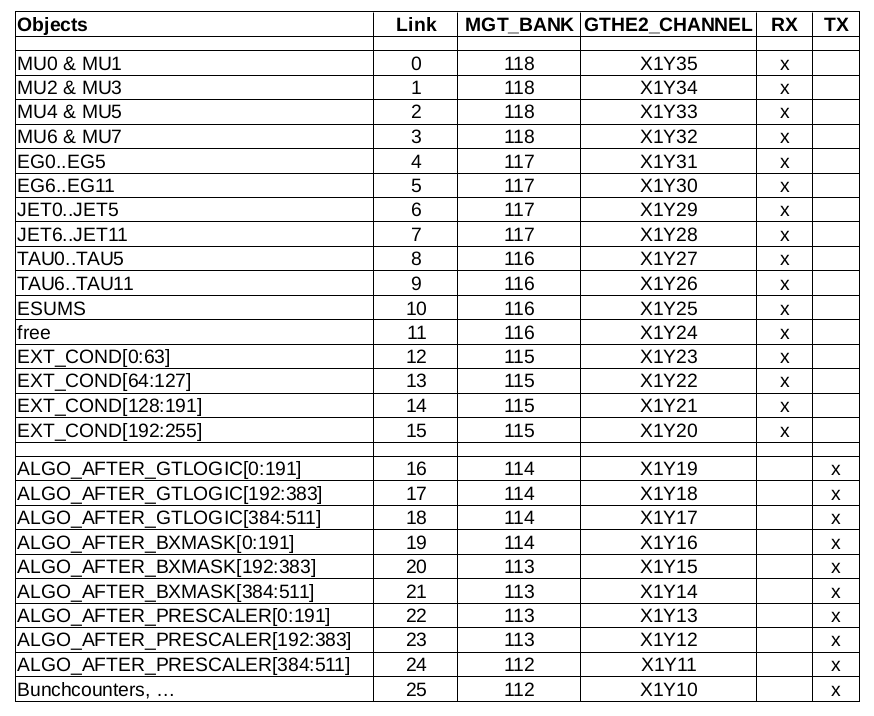
\includegraphics[width=15cm]{figures/gth_xc7v690t_ffg1927}
\caption{Configuration of GTHs}
\label{fig:app:gth_conf}
\end{figure}

\clearpage

\subsection{Configuration of optical links}\label{sec:app:app_b}
% \textbf{Appendix B:}

Figure~\ref{fig:app:ugt_inputs} shows the configuration of optical links to Global Trigger.\\
Links 0..3 contains muon data from GMT, links 4..11 data from GCT and links 12..15 external conditions
from AMC502 boards.

\begin{figure}[htb]
\centering
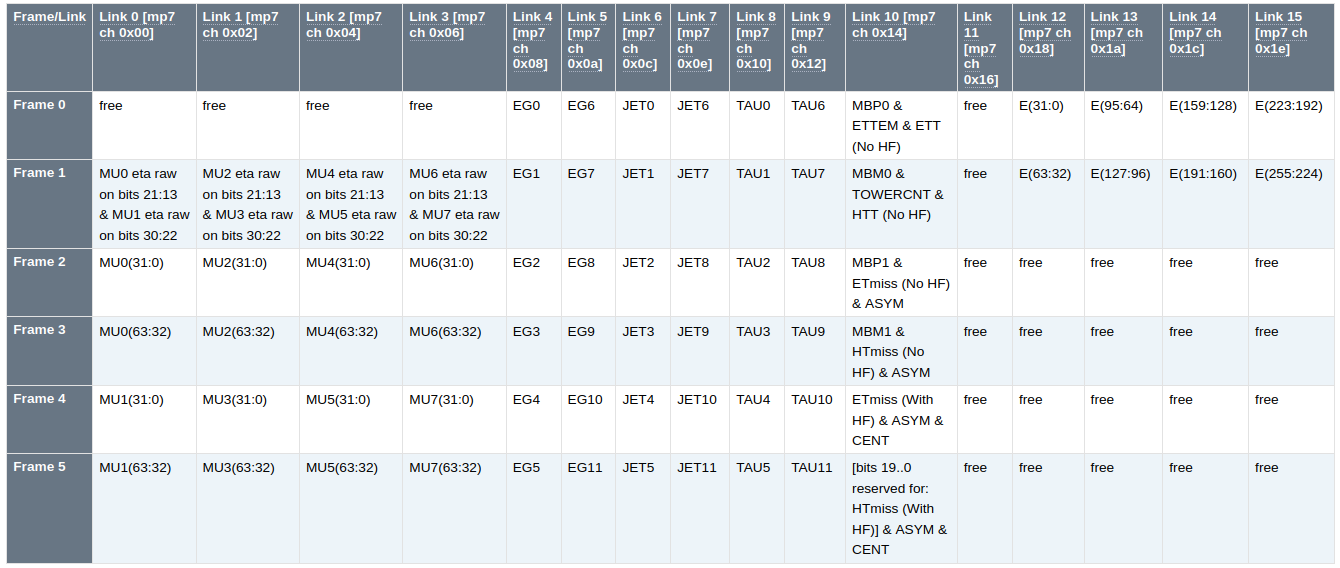
\includegraphics[width=15cm]{figures/ugt_inputs}
\caption{Optical link inputs to Global Trigger}
\label{fig:app:ugt_inputs}
\end{figure}

\subsection{Configuration of links to AMC13 (readout)}\label{sec:app:app_c}
% \textbf{Appendix C:}

Figure~\ref{fig:app:ugt_outputs} shows the configuration of links from Global Trigger to AMC13 (readout).\\
Links 16..24 contains algo data (after GTL, after BX mask and after prescalers), link 25 contains several counter values.

\begin{figure}[htb]
\centering
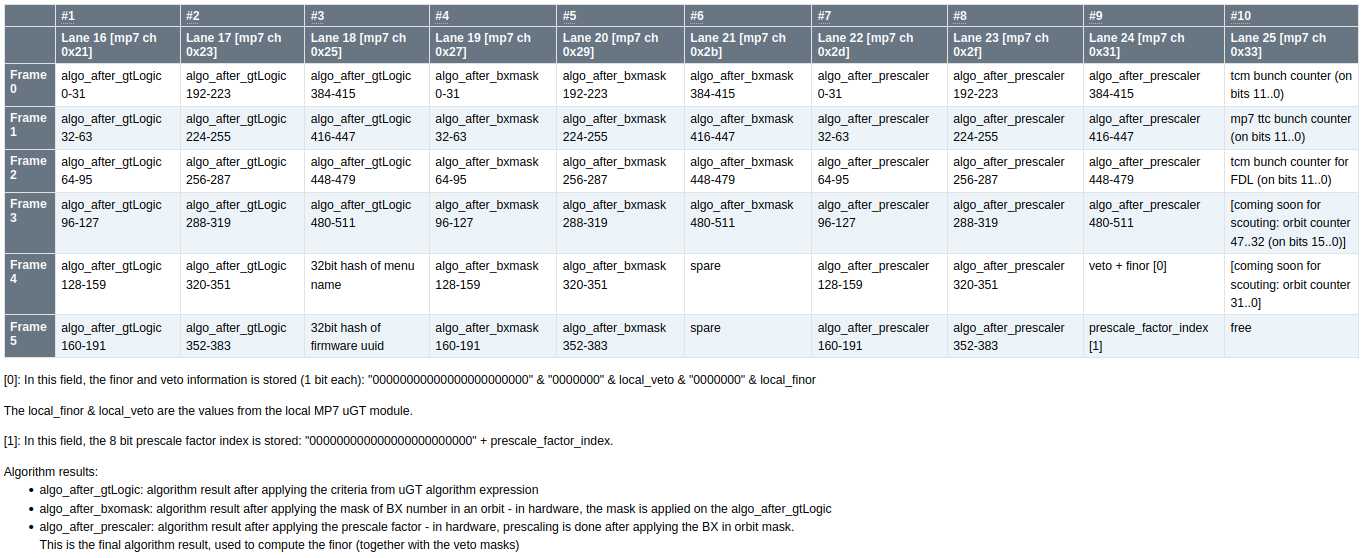
\includegraphics[width=15cm]{figures/ugt_outputs}
\caption{Outputs from Global Trigger to AMC13}
\label{fig:app:ugt_outputs}
\end{figure}

\clearpage

\subsection{Optical patch panel}\label{sec:app:app_d}
% \textbf{Appendix D:}

Figure~\ref{fig:app:ugt_pp} shows the connections on Global Trigger patch panel for optical links.

\begin{figure}[htb]
\centering
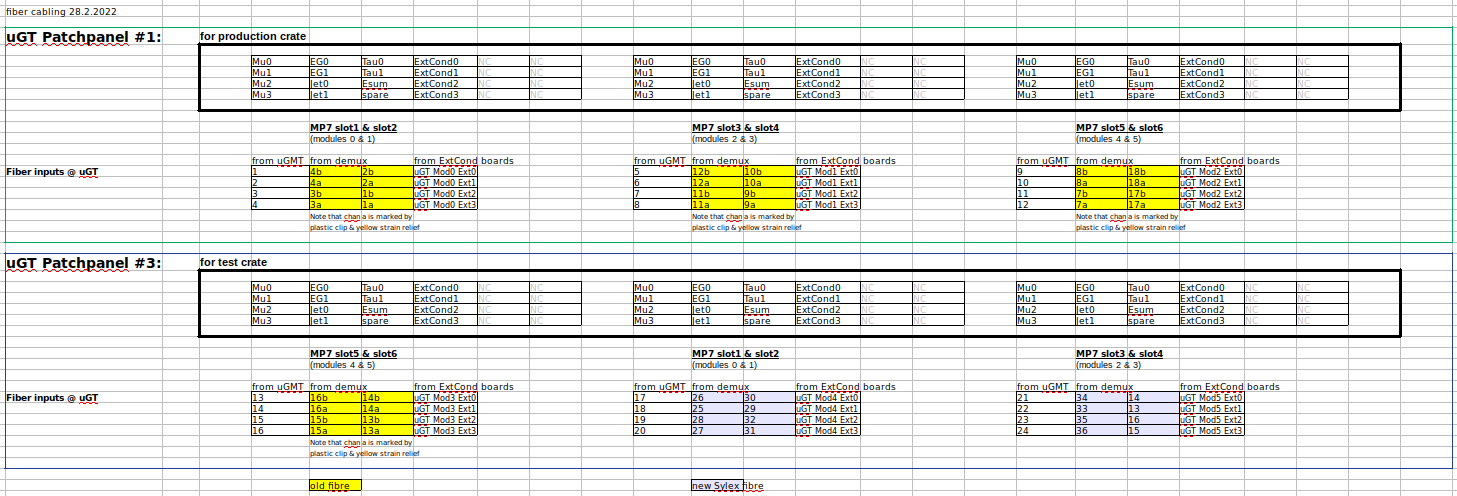
\includegraphics[width=15cm]{figures/ugt_patchpanel}
\caption{Global Trigger patch panel for optical link}
\label{fig:app:ugt_pp}
\end{figure}

\subsection{Description of tests}\label{sec:app:app_e}
% \textbf{Appendix E:}

Workflow for simulation and synthesis of firmware is described in \href{\gitbranch/README.md}{\texttt{README}} file.\\\\
List of useful TDF routines and commands for hardware tests:
\begin{itemize}
\item Load firmware to scansd card on all MP7 modules and load it into FPGAs\\
\textit{\small{\$ tdf run uploadfw\_gt <tar file path> --rebootfpga}}
\item Load firmware from scansd card into FPGA\\
\textit{\small{\$ tdf run loadfw\_gt <fw build nr> <nr modules>}}
\item Compare hardware results with test vector pattern\\
\textit{\small{\$ tdf run multiboard\_function\_test -h}}
\item Enable TTC signals on AMC13 for all MP7 modules\\
\textit{\small{\$ tdf run ttc\_enable\_all}}
\item Check lock of BC0 and LHC clock\\
\textit{\small{\$ tdf unittest <module> default}}
\item Check minipods\\
\textit{\small{\$ tdf mp7butler minipods <module>}}
\item ...\\
\end{itemize}

\clearpage


% List of tables.
\doctables{}

% List of figures.
\docfigures{}

% \section*{Acronyms}
% \begin{acronym}
% \section{Acronyms}\label{sec:acronyms}

\begin{acronym}
\acro{AMC13}{AMC board in uTCA crate for several features (readout, ...)}
\acro{DAQ}{Data Acquisition}
\acro{FDL}{\fdl Module}
\acro{GCT}{Calorimeter~Trigger~Layer-2}
\acro{GMT}{\gmt}
\acro{GT}{\gt}
\acro{GTL}{\gtl Module}
\acro{ROP}{Readout Process Module}
\acro{TCM}{Timing Counter Manager Module}
\acro{TCDS}{Trigger, Control and Distribution System}
\end{acronym}

\clearpage



% \end{acronym}

\clearpage

\begin{thebibliography}{00}

\bibitem {MP7}
MP7 documentation:\\
\url{http://www.hep.ph.ic.ac.uk/mp7}

\bibitem {MP7 firmware}
MP7 firmware repository:\\
\url{https://gitlab.cern.ch/cms-cactus/firmware/mp7}

\bibitem {TME_repo}
Trigger Menu Editor repository:\\
\url{https://github.com/cms-l1-globaltrigger/tm-editor}

\bibitem {VHDL_Producer}
VHDL Producer repository:\\
\url{https://github.com/cms-l1-globaltrigger/tm-vhdlproducer}

% \bibitem {muon}
% \url{http://www.hephy.at/project/cms/trigger/globalMuonTrigger/notes/in04\_006.pdf}

\bibitem {interface}
Calo-layer2 and Global Muon Trigger interface documentation:\\
\url{https://raw.githubusercontent.com/cms-l1-globaltrigger/mp7_ugt_legacy/master/doc/scales_inputs_2_ugt/pdf/scales_inputs_2_ugt.pdf}

\bibitem {GTHs}
Xilinx Series 7 Transceivers (GTHs) documentation:\\
\url{https://www.xilinx.com/support/documentation/user_guides/ug476_7Series_Transceivers.pdf}

\end{thebibliography}

% % Index.
% \docindex{}

% End of document structure.
\end{document}

% eof
